%!TEX TS-program = xelatex
%!TEX encoding = UTF-8 Unicode

\documentclass[School=EMC]{Dissertate}
\usepackage{tikz}
\usepackage[sectionbib]{chapterbib}
\usepackage{tabularx}
\usepackage{enumitem}
\usepackage[none]{hyphenat}
\usepackage{subcaption}
\usepackage{graphicx}
\usepackage{wrapfig}
\usepackage[hyphens]{xurl} % fixes url splitting over lines
\usepackage[paperwidth=18.0cm, paperheight=25.0cm, left=2.5cm,right=2.5cm,bottom=3cm,top=3cm]{geometry}
%\usepackage[width=6.75in, letterpaper, bottom=3cm, top=3cm]{geometry}
%\newcommand\bookepigraph[4]{
%\vspace{1em}\hfill{}\begin{minipage}{#1}{\begin{spacing}{0.9}
%\small\noindent\textit{#2}\end{spacing}
%\vspace{1em}
%\hfill{}{#3}\\

%\vspace{-1em}\begin{flushright}{#4}\end{flushright}}\vspace{2em}
%\end{minipage}}

\def\changemargin#1#2{\list{}{\rightmargin#2\leftmargin#1}\item[]}
\let\endchangemargin=\endlist

\newcommand\epigraph[3]{
    \vspace{1em}\begin{center}
    \begin{minipage}{#1}{
        \begin{spacing}{1.2}
        \small\noindent\textit{#2}\end{spacing}
        \vspace{1em}
        \hfill{}\small{#3}
    }
    \vspace{2em}
    \end{minipage}
    \end{center}
}



%\newcommand\anonymousepigraph[2]{
%\vspace{1em}\hfill{}\begin{minipage}{#1}{\begin{spacing}{0.9}
%\small\noindent\textit{#2}\end{spacing}}
%\vspace{1em}
%\end{minipage}}
\usetikzlibrary{calc}

% Orange
\definecolor{title1}{HTML}{8c0000}
\definecolor{title2}{HTML}{ff3c00}
\definecolor{title3}{HTML}{b90000}
\definecolor{title4}{HTML}{ff8080}

% Blue
\definecolor{title1}{HTML}{8c0000}
\definecolor{title2}{HTML}{003cff}
\definecolor{title3}{HTML}{0000b9}
\definecolor{title4}{HTML}{8080ff}


% hyphenation
\usepackage[british]{babel}
\babelhyphenation[british]{bio-infor-ma-tician}
\babelhyphenation[british]{bio-infor-ma-ticians}
\babelhyphenation[british]{bio-infor-ma-tics}
\setlength\emergencystretch{3em}

% ensuring certain pages appear on left or right side
\newcommand*\cleartorightpage{%
  \clearpage
  \ifodd\value{page}\hbox{}\newpage\fi
}

\newcommand*\cleartoleftpage{%
  \clearpage
  \ifodd\value{page} \else \hbox{}\newpage \fi
}


%%%%%%%%%%%%%%%%%%%%%%%%%%%%%%%%% Thumb index

\usepackage[contents={},opacity=1,scale=1,color=black]{background}
\usepackage{tikzpagenodes}
\usepackage{totcount}
\usetikzlibrary{calc}

\newif\ifMaterial

\newlength\LabelSize
\setlength\LabelSize{2.5cm}

\AtBeginDocument{%
\regtotcounter{chapter}
\setlength\LabelSize{\dimexpr\textheight/\totvalue{chapter}\relax}
\ifdim\LabelSize>2.5cm\relax
  \global\setlength\LabelSize{2.5cm}
\fi
}

\newcommand\AddLabels{%
\Materialtrue%
\AddEverypageHook{%
\ifMaterial%
\ifodd\value{page} %
  \backgroundsetup{
  angle=90,
  position={current page.west|-current page text area.north west},
  vshift=-15pt,
  hshift=-\thechapter*\LabelSize,
  contents={%
  \tikz\node[fill=gray!30,anchor=west,text width=\LabelSize,
    align=center,text height=15pt,text depth=10pt,font=\large\sffamily] {\thechapter};
  }%
 }
 \else
 \backgroundsetup{
  angle=90,
  position={current page.east|-current page text area.north  east},
  vshift=15pt,
  hshift=-\thechapter*\LabelSize,
  contents={%
  \tikz\node[fill=gray!30,anchor=west,text width=\LabelSize,
    align=center,text height=15pt,text depth=10pt,font=\large\sffamily] {\thechapter};
  }%
 }
 \fi
 \BgMaterial%
\else\relax\fi}%
}

\newcommand\RemoveLabels{\Materialfalse}

%%%%%%%%%%%%%%%%%%%%%%%%%%%%%%%% End Thumb index


\begin{document}

% the front matter
%\begin{titlepage}
%\usepackage{tikz}
\tikz[remember picture,overlay]
\node[opacity=0.8,inner sep=0pt] at (current page.center){
    
\includegraphics[width=\paperwidth,height=\paperheight]{frontmatter/images/cover2.jpg}
};
%\clearpage

\begin{center}

\color{white}{
\vspace{-2cm}
\huge{
    \sc{
    \textbf{ \uppercase{The Big Red Button}}} \\
    \normalsize toward the biologist's dream of a mystical button converting raw data into Nature papers

    \vspace{16.6cm}

    \LARGE Saskia Hiltemann}
}
\end{center}
\end{titlepage}

\begin{titlepage}
%\usepackage{tikz}
\tikz[remember picture,overlay]
\node[opacity=0.4,inner sep=0pt] at (current page.center){
    
\includegraphics[width=\paperwidth,height=\paperheight]{frontmatter/images/puzzle-texture.jpg}
};
%\clearpage

% top band
\begin{tikzpicture}[remember picture,overlay]
  %\fill[title1] ($(current page.north west)-(0cm,3cm)$) rectangle (current page.east);
   \shade[left color=title2,right color=title3] (-3,-1) rectangle (\paperwidth, 3);

% bottom band
   \shade[left color=title2,right color=title4] (-3,-22) rectangle (\paperwidth, -18);
\end{tikzpicture}


\begin{center}

\vspace{-3cm}
\begingroup
    \fontsize{36pt}{12pt}\selectfont
    \color{white}{\textbf{ \sc{The Jigsaw Genome}}} \\
\endgroup


\large \sc{ \color{white}{demystifying bioinformatics through open and accessible community-driven practices}}\\

\vspace{1.5cm}
\begin{figure}[h!]
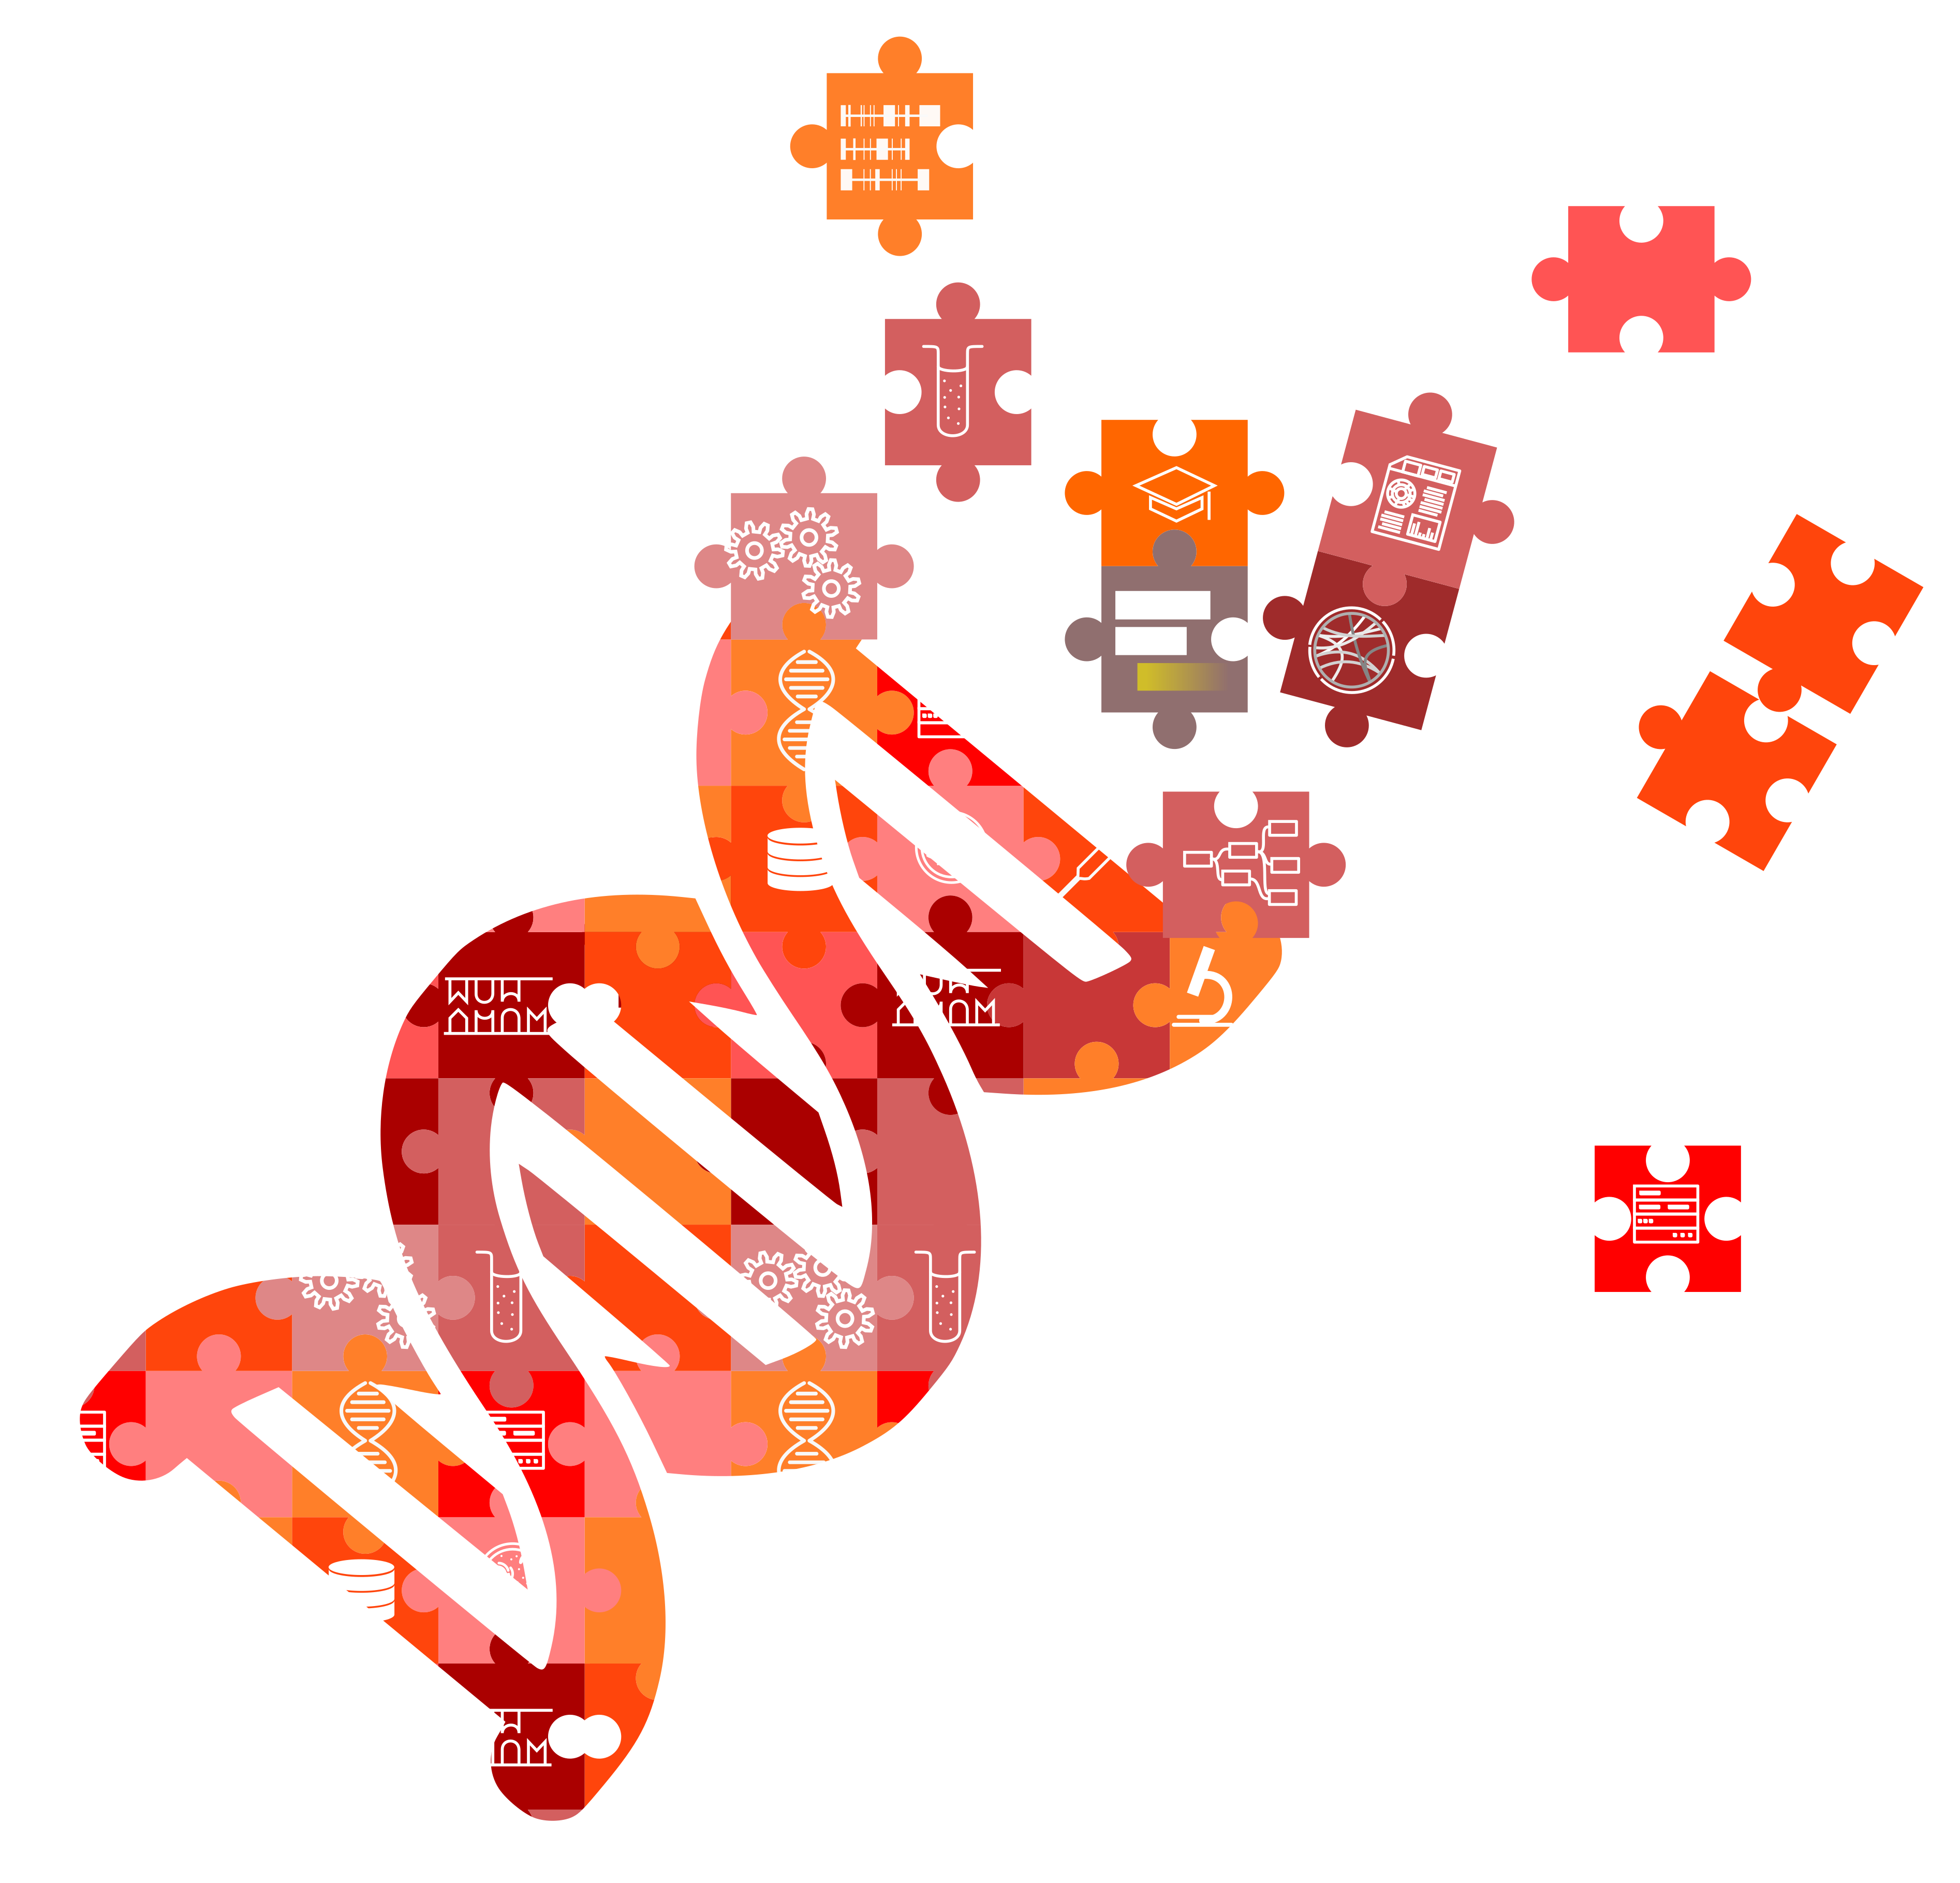
\includegraphics[scale=0.6]{frontmatter/images/cover-puzzle-helix-export.png} \\
\end{figure}

\vspace{2cm}
\begingroup
    \fontsize{36pt}{12pt}\selectfont
    \color{white}{Saskia Hiltemann}
\endgroup
\end{center}

\end{titlepage}

%\newpage \thispagestyle{empty} This page was intentionally left blank. %\newpage
%\begin{titlepage}
%\usepackage{tikz}
%\tikz[remember picture,overlay]
%\node[opacity=0.4,inner sep=0pt] at (current page.center){
    %
\includegraphics[width=\paperwidth,height=\paperheight]{frontmatter/images/puzzle-texture.jpg}
%};
%\clearpage

\tikz[remember picture,overlay] \node[opacity=1,inner sep=0pt] at (current page.center){
\includegraphics[width=\paperwidth,height=\paperheight]{frontmatter/images/cover-puzzle.png}};
\enlargethispage{4cm}

% top band
%\begin{tikzpicture}[remember picture,overlay]
  %\fill[title1] ($(current page.north west)-(0cm,3cm)$) rectangle (current page.east);
  % \shade[left color=title2,right color=title3] (-3,-1) rectangle (\paperwidth, 3);

% bottom band
%   \shade[left color=title2,right color=title4] (-3,-22) rectangle (\paperwidth, -18);
%\end{tikzpicture}


\begin{center}

\vspace{-1.5cm}
\begin{changemargin}{1cm}{-8cm}
\begingroup
    \fontsize{34pt}{12pt}\selectfont
    \hspace{-2cm}\color{white}{\textbf{\sc{Bioinformatics for Everyone}}} \\
\endgroup
\hspace{-3cm}\large \sc{\color{white}{demystifying bioinformatics through open and accessible community-driven practices}}\\
\end{changemargin}

\vspace{16.9cm}
\begingroup
	\fontsize{36pt}{12pt}\selectfont
	{\hspace{6cm}{\color{white}Saskia}\ \\[0.7cm]\hspace{6.5cm}\color{white}Hiltemann}
\endgroup
\end{center}

\end{titlepage}

%\begin{titlepage}
%\usepackage{tikz}
\tikz[remember picture,overlay]
\node[opacity=0.1,inner sep=0pt] at (current page.center){
    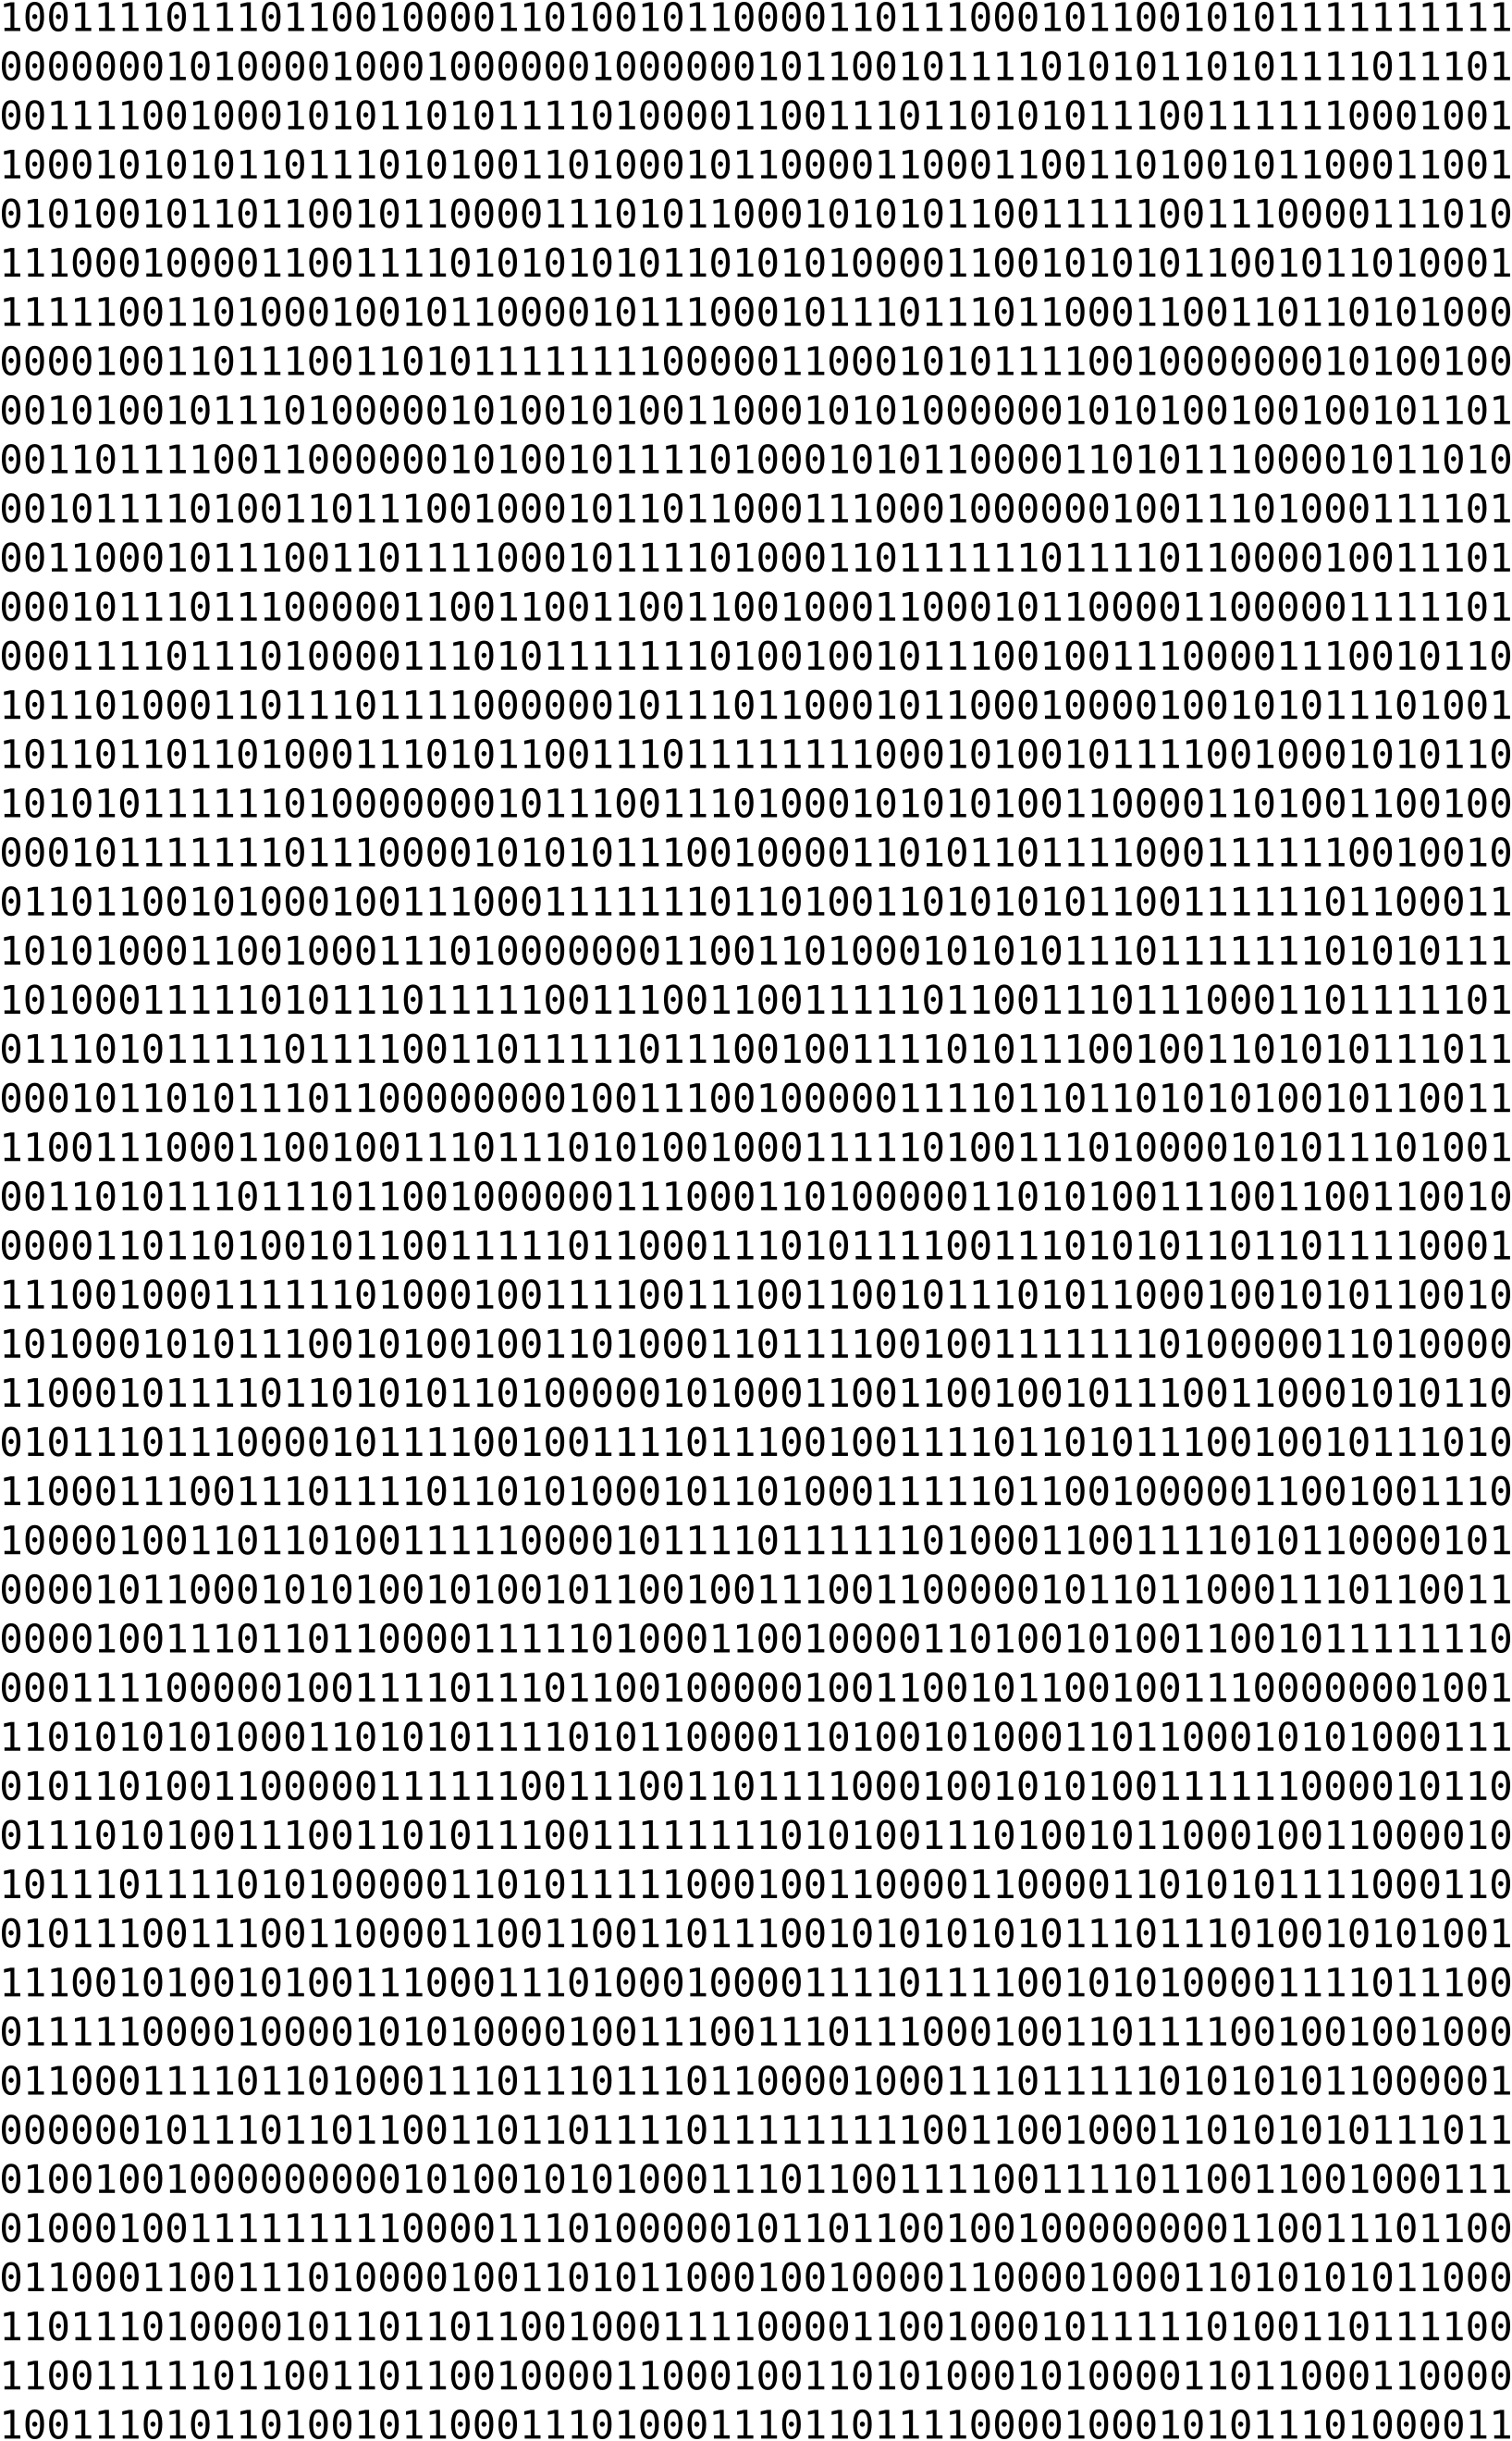
\includegraphics[width=\paperwidth,height=\paperheight]{frontmatter/images/binary.png}
};
%\clearpage

\begin{center}

\color{black}{
\vspace{-2cm}
\huge{
    \sc{
    \textbf{ \uppercase{The Big Red Button}}} \\
    \large toward the biologist's dream of a mystical button converting raw data into Nature papers

    \vspace{4cm}
    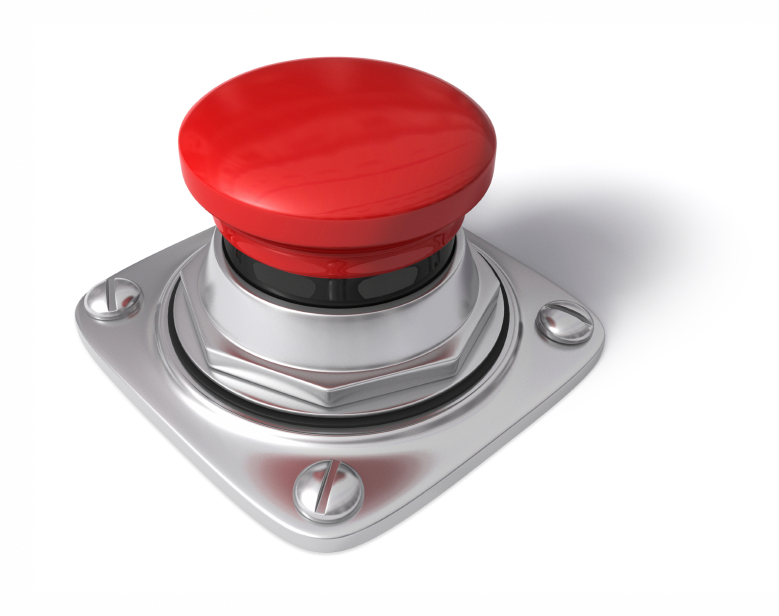
\includegraphics[scale=0.4]{chapters/images/redbutton.png}
    \vspace{4cm}

    \LARGE Saskia Hiltemann}
}
\end{center}
\end{titlepage}

%\begin{titlepage}
%\usepackage{tikz}
\tikz[remember picture,overlay]
\node[opacity=0.5,inner sep=0pt] at (current page.center){
    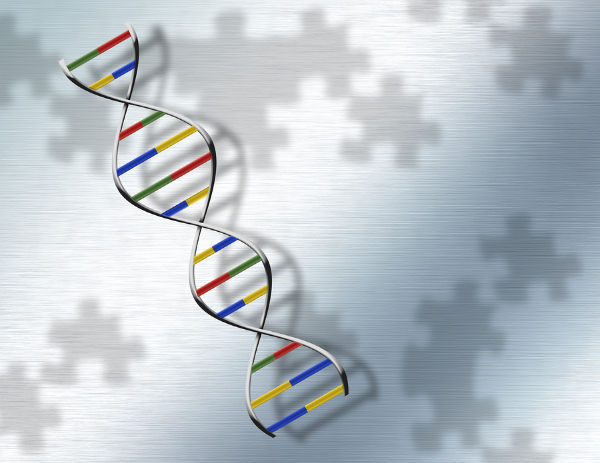
\includegraphics[width=\paperwidth,height=\paperheight]{frontmatter/images/jigsaw_genome5.jpg}
};
%\clearpage

\begin{center}

\color{black}{
\vspace{-2cm}
\huge{
    \sc{
    \textbf{ \uppercase{The Jigsaw Genome}}} \\
    \large solving the puzzle that is genomics

    \vspace{16.6cm}

    \LARGE Saskia Hiltemann}
}
\end{center}
\end{titlepage}


% Some details about the dissertation.
%\cleartorightpage
\title{Jigsaw Genomics}
\subtitle{Assembling the pieces toward open and accessible bioinformatics for all}
\titledutch{Jigsaw Genomics}
\subtitledutch{De puzzelstukjes op hun plaats leggen voor open en toegankelijke bioinformatica voor iedereen}
\author{Saskia Hiltemann}
\advisor{Bigname Scientist}
\rector{Prof.dr. R.C.M.E. Engels}
\defensedate{XX YY 2020}
\defensetime{00:00 uur}
\placeofbirth{Tilburg, Nederland}

% ... about the degree.
\degree{Doctor of Philosophy}
\field{Bioinformatics}
\degreeyear{2024}
\degreemonth{May}
\department{Bioinformatics}

% ... about the candidate's previous degrees.
\pdOneName{B.S.}
\pdOneSchool{Boston University}
\pdOneYear{2018}

\pdTwoName{M.A.}
\pdTwoSchool{Monster's Univeristy}
\pdTwoYear{2021}

\maketitle


%\copyrightpage
%\abstractpage
\dedicationpage

\setcounter{page}{0}

\begin{justify}
% the abstract
\chapter*{Foreword}
\setlength\parindent{0pt}
\vspace{-1cm}
I like puzzles. Any type of puzzle. I always have. If I see a puzzle or a problem I have
to solve it. I think that is what makes cancer such a fascinating topic for me.

Imagine you are given a jigsaw puzzle. Now instead of a few hundred pieces, there are
several billion pieces. The picture on the box is not a picture of the puzzle inside the box,
it is just a somewhat similar image. Oh, and did I mention there are a whole bunch
of pieces missing? and that many pieces are duplicated? Some pieces don't even belong in our box,
but come from a completely different puzzle. On top of that your little sister has spilled paint
over some of the pieces so those can't be trusted to contribute to the image. And instead of one
single puzzle, the box contains several, they are all variations of the image on the box, but you have
no idea how many different puzzles the box contains.

Sound challenging? This is the problem we are solving whenever we sequence a cancer genome.

\vspace*{0.5cm}
\textbf{[Metaphor key]} \\
\textit{puzzle pieces} = sequence reads \\
\textit{picture on box} = reference genome \\
\textit{missing pieces} = hard-to-sequence areas \\
\textit{other puzzles} = contamination \\
\textit{painted pieces} = sequencing errors \\
\textit{multiple puzzles in box} = clonality

\verb+<thought: have the metaphor low-key run throughout thesis? >+

%\chapter*{Stellingen}

(TODO: remove, just a placeholder for notes and ideas)


Eleven propositions must be added to the doctoral dissertation. Of these propositions,
five must relate to the contents of the doctoral dissertation and five must not relate,
either directly or indirectly, to the contents of the doctoral dissertation. These ten
propositions must be academically defensible. The eleventh proposition does not have
to meet the criterion of academic defensibility. The doctoral candidate must submit the
propositions to the doctoral dissertation supervisor as soon as possible following the
approval of the doctoral dissertation as referred to in Article 5.1.

\begin{itemize}
\item 5 from thesis, academically defensible
\item 5 unrelated to thesis, academically defensible
\item 1 anything goes, academically defensible or not
\end{itemize}

\begin{comment}
ideas

\begin{itemize}
\item This manuscript
    \begin{itemize}
    \item Training is pivotal

    \end{itemize}
\item Academia
    \begin{itemize}
     \item Scientists should write up results for general public as well as scientific journals
     \item Open science FTW, no more paywalled journals. or use money to pay peer reviewers to do thorough testing. or professional reviewers.
     \item Do we even need journals? system of completely open peer review could replace
     \item post-publication public peer review FTW
    \end{itemize}
\end{itemize}
\end{comment}

\end{justify}

%TODO: remove
%\chapter*{Scope of Thesis}

Chapter 1: General technical papers useful for many studies: Galaxy, iReport, Circos? \\
Chapter 2: Training Materials \\
Chapters 3-5: Technical paper \& the biological insight it led to/facilitated \\

\begin{enumerate}
    \item Tools: Galaxy, iReport, Circos(?)
    \item Training Materials
    \item Cancer - Fusion Gene detection: iFUSE \& VCaP Chromothripsis
    \item Cancer - Somatic Variant detection: CGtag \& Virtual Normal
    \item Microbiota profiling: GmT \& MYcrobiota
\end{enumerate}


\setlength\cftparskip{-5pt}
\setlength\cftbeforechapskip{0pt}

\setcounter{tocdepth}{1}
\tableofcontents
%\phantomsection
%\addcontentsline{toc}{chapter}{Table of Contents}


%\authorlist
%\listoffigures

%\abstractpage
%\doublespacing


% start chapter and page numbering at 0 because (computer) science
\setcounter{chapter}{-1}


% include each chapter...
\AddLabels % start using thumb index
\chapter{Introduction}
\label{introduction}
 % start numberings at 0 because (computer) science
\setcounter{figure}{-1}
\setcounter{table}{-1}
\setcounter{section}{-1}
\setcounter{NAT@ctr}{-1}

\setlength\parindent{0pt}


\begin{comment}
\section*{Contents}
\begin{enumerate}
\itemsep-0.5em
\item A Brief History of Genomics
\item A Primer on Sequencing (?)
\item The Bioinformatics Challenge
\item Bioinformatics Best Practices
\item The Galaxy Platform
\item Use case 1: Prostate Cancer
\item Use case 2: Microbiota Analysis
\item Scope of this Thesis.
\end{enumerate}
\end{comment}


\section{The Source Code of Life}

DNA. The blueprint of life. These long double-stranded helical molecules are present in all living cells on earth\footnote{As far as currently known. Some viruses contain only RNA, but these are often not considered "alive".} and encode the proteins which drive the functioning, regulation, structure and replication of the cells and tissues that make up an organism. In many ways, DNA is also analogous to computer code; any computer program, no matter how complex, can be described as a long series of just two characters, \verb+0+ and \verb+1+, known as \emph{bits}. Knowing the sequence of these bits and, crucially, the details about how they are being interpreted by the machine on which they are executed, lets us understand and predict the functions they encode. In much the same way, DNA uses just 4 different elements, called \emph{bases} or \emph{nucleotides}, to encode its blueprint for the cell. These 4 building blocks are adenine, cytosine, guanine and thymine, usually referred to simply by their first letters, \verb+A+, \verb+C+, \verb+T+ and \verb+G+. These bases combine together in pairs (\emph{base pairs}), with \verb+A+ always matching to \verb+T+ and \verb+C+ being complementary to \verb+G+ along a sugar phosphate backbone in their double-helix configuration (Figure \ref{fig:dnastructure}).

\begin{wrapfigure}{r}{210pt}
%\begin{figure}[h!]
    \centering
    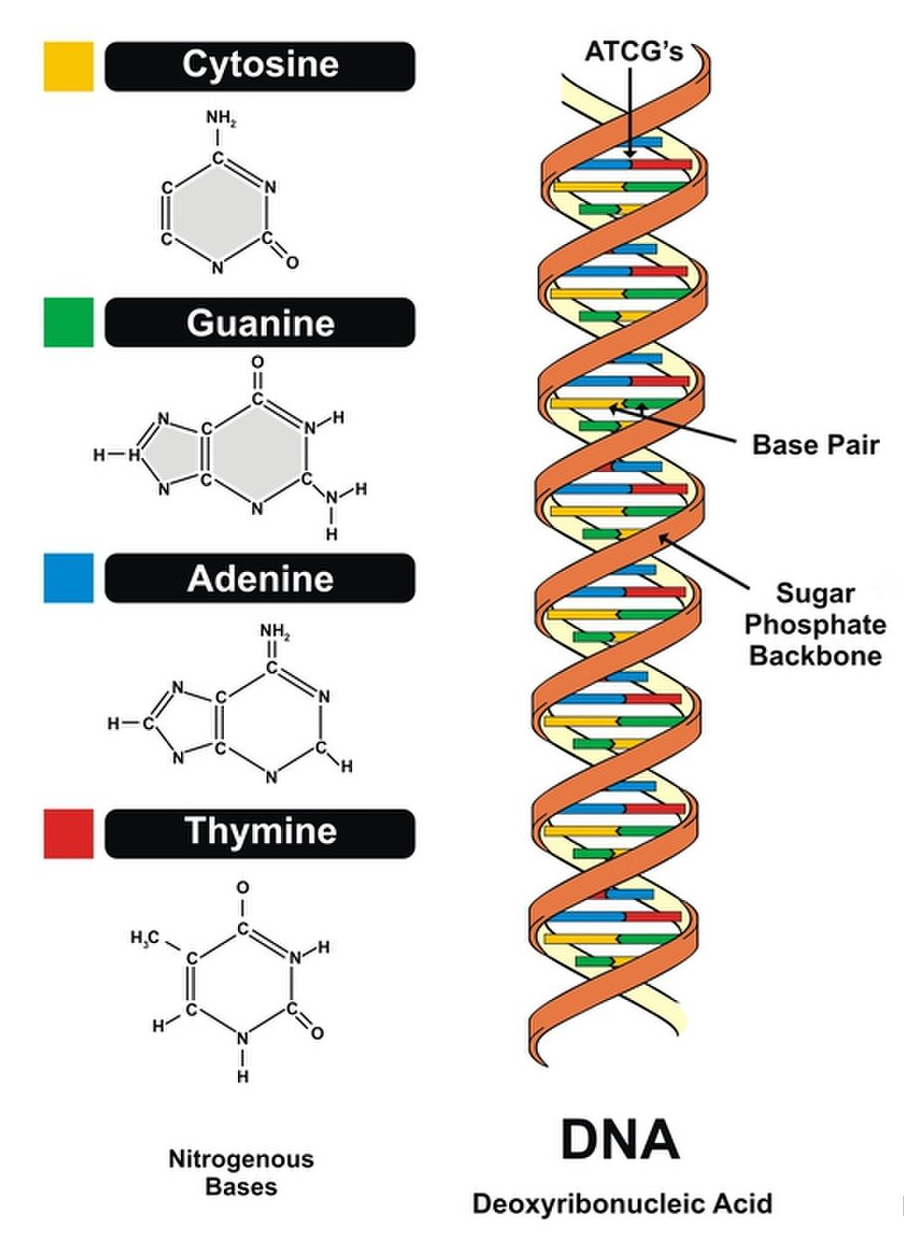
\includegraphics[width=200pt]{chapters/images/introduction/dna-structure.png}
    \caption{Structure of DNA}
    \label{fig:dnastructure}
%\end{figure}
\end{wrapfigure}

In humans, DNA is organised into 23 pairs of chromosomes, with a total length of over 3 billion base pairs. About 1\% of this DNA make up \emph{genes}; stretches of DNA which directly encode protein molecules. When these genes are expressed, the gene sequence is transcribed to a messenger molecule (\emph{mRNA}) which is subsequently translated into a protein molecule. The function of the remaining 99\% of the genome long remained a mystery, and was even referred to as \emph{junk DNA}. More recent studies have revealed that these stretches of non-coding DNA play an important role in the regulation of the expression of genes, stimulating or prohibiting the translation of genes to proteins and thereby influencing the functioning of the cell. For any two individuals, the vast majority of their DNA sequence will be identical, but small variations in the remaining locations of the genome are what make each of us unique. But it is also what can make us sick. Studying this natural variation in the genome sequence helps us unravel the mechanisms of life and disease.


\subsection{A Brief History of Genome Sequencing}
Friedrich Miescher was the first to isolate DNA molecules (which he termed \emph{nuclein}) in 1869. However, the molecule remained relatively understudied until Rosalind Franklin used X-ray crystallography to inspect the molecule's structure \cite{elkin2003rosalind}. Watson and Crick famously used this data to postulate the double-helix model of DNA in 1953 \cite{watson1953molecular}. This model illustrated for the first time that DNA molecules we ideally suited for replication, and solidified the idea that DNA, and not protein as was previously thought, was the primary carrier of hereditary information. Simultaneously, Frederick Sanger had developed techniques to sequence proteins, and later RNA and DNA molecules. This was the start of first generation of genome sequencing, and the first full gene was sequenced in 1972 () \cite{TODO}, followed by the first full genome in 1976 (bacteriophage Phi X 174, 5386 nucleotides long) \cite{}. These early techniques were only suitable for relatively small sections of DNA, and more technological advances would be required before larger genomes could be fully sequenced.

In 1990, the Human Genome Project \cite{olson1993human} set out to sequence the entire 3.2-billion-basepair-long human genome, an effort culminating in 2003 with the publication of the first human \textit{reference genome} \cite{international2004finishing}. Not only did this provide invaluable insights into human genetics, but it also paved the way for the next era in genetic research; something which would completely transform the field of genetic research. Over the next several years, next-generation massively parallel sequencers were developed by companies like Roche454 and Illumina, dramatically cutting the cost and time required to sequence a human genome, and for the first time demonstrated its potential utility in clinical and diagnostic settings. Through sustained technological advancements over the following years, these costs continued to decrease at exponential rates - outstripping even the pace predicted by Moore's law (\hyperref[fig:seqcost]{Fig. \ref{fig:seqcost}}) - and the long dreamed-about \textit{\$1,000 dollar genome} \cite{thousanddollargenome} \cite{sequencingcostsNHGRI} has now become a reality.

\begin{figure}[h!]
    \centering
    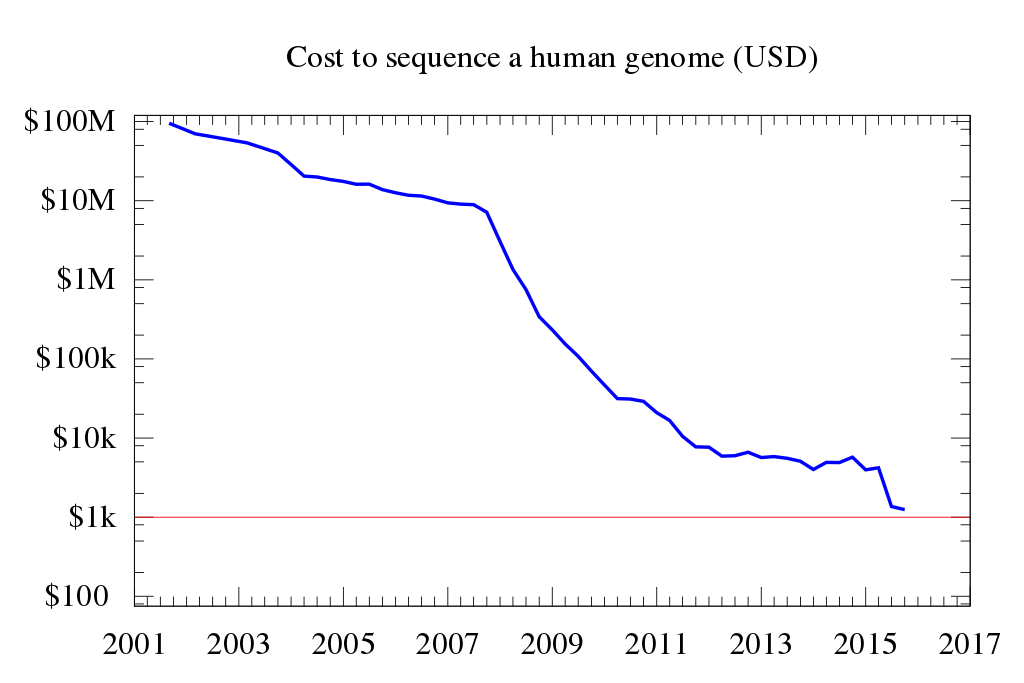
\includegraphics[width=300pt]{chapters/images/Historic_cost_of_sequencing_a_human_genome.png}
    \caption{The cost of sequencing a human-sized genome over time. Data from the NHGRI Genome Sequencing Program (GSP) }
    \label{fig:seqcost}
\end{figure}

Shortly after the publication of the human genome, high-throughput techniques emerged to also sequence the transcriptome (RNA-Seq), allowing for the identification and quantification of gene transcripts, and providing information about post-transcriptional mutations and other complexities such as alternative splicing \cite{wang2009rna}. Similarly, the study of epigenetics is revealing that non-coding DNA, far from the once-termed \textit{"junk DNA"}, is part of an intricate and complex regulatory system controlling the expression of genes \cite{zuckerkandl2007combinatorial}.

Now we are now moving into the era of third-generation sequencing, where single-cell \cite{gawad2016single}, long-read \cite{koren2015one}, and often real-time sequencing \cite{flusberg2010direct} are allowing for ever more accurate determination of nucleotide sequence, providing increased resolution even in highly diverse and complex samples such as cancer or metagenomic samples. All these technological advances have led to a deluge of data that must be managed and analysed, typically by bioinformaticians.


\section{The Bioinformatics Challenge}

With huge amounts of data now being generated at relatively low cost \cite{chen2014big}, and compute resources being available even on moderate budgets, the challenge in genomic research has shifted from the sequencing technologies to the analysis and interpretation of these big and highly complex datasets, and the development of the software required to do so, in order to gain new understanding of the underlying biological systems. This poses a significant challenge, both technologically and scientifically.

\subsection{Ever-changing landscape}
Sequencing technologies are evolving at a staggering pace, and with them, so must the software tools capable of analysing the data. Therefore, new tools are developed continually and existing tools must be updated regularly to remain relevant. As a consequence, there typically simply is not enough time for community standards and consensus analysis pipelines to emerge organically before the advent of new technologies make them obsolete. Because of this, there usually are a multitude of tools available for any given task, each with their own set of advantages and disadvantages, and the challenge is to find the right tool for the particular situation, and knowing when to use existing tools and when the development of novel tools is in order.

\subsection{Standardisation}
Such a lack of clear standards does not only apply to software tools, but also to file formats, and this poses a major hurdle in data analysis. While some clear data format standards exist [fastq, VCF], there are many cases that lack such a standard, hindering the interoperability of different tools. And even the more established file formats such as fastq and VCF allow for a variety of flavours, e.g. different fastq quality encoding schemes, which are not indicated inside the file format specification itself, but may influence downstream results. Thus, when creating analysis pipelines from existing tools, many file transformation steps are typically required as a kind of \textit{glue} between steps.

\subsection{Data Storage}
 \begin{comment} https://qumulo.com/blog/genomic-sequencing-qf2-storage/ \end{comment}
Sequencing data is being generate at a rate of X petabytes per year (TODO: find citation), and all this data must be stored somewhere. But there is more to data storage than buying a hard disk and copying data. The data must be backed up to prevent data loss, it must be made available for use in an efficient way (I/O matters), data must be organised and tracked in a usable manner, and any solution must be able to scale to the exponential trend of growth both in size and number of files generated. Furthermore, data storage must comply with privacy and security requirements, especially important in the case of human genetic data.


\subsection{The Specialist Bioinformatician}
All of these challenges have resulted in bioinformatics becoming a highly specialized field, which in itself poses a new challenge given the observation that the domain knowledge (biology) and the informatics know-how more and more often do not reside in a single individual, and the interpretation of the data cannot always be done by the person performing the data analysis and vice versa. Instead, close communication between the two fields is required, and the domain experts should be empowered to perform their own data analyses as much as possible.

\verb+informatician needs to shine a light in the black box that is the wetlab, domain expert needs to become comfortable with the informatics, since this has become an integral part of any analysis+


% some (partial) solutions to the above challenges, spoilers: open software, open science, open everything
\section{Bioinformatics Best Practices}
Since bioinformaticians are primarily academics -who are typically being judged on their publications, not their code-, the quality of bioinformatics tools is highly variable and tool authors often struggle to find the time and resources to maintain their code. The open-source community is instrumental in this respect, allowing the most popular and useful tools to be taken up by the community which can collectively maintain and update the bioinformatics software packages. Adhering to a set of best-practices guidelines can greatly reduce this maintenance burden, and increase the chance of tools being taken up by the community.

Many journals require authors to submit datasets to public repositories in order to allow other scientists to reproduce their findings. With bioinformatics now such a fundamental part of any publication, a clear description of the analysis pipeline is also required for true reproducibility, but the majority of scientific publication do not contain all the information required to reproduce the in-silico experiment [cite]. Making analysis software open-source and adhering to a set of bioinformatics best-practices can improve the reproducibility of bioinformatics analysis pipelines.

Such bioinformatics best-practices include:

\begin{enumerate}
    \itemsep-0.5em
    \item Accessibility of tools and data %(usability) of tools (documentation, open source, github etc, galaxy, galaxy, dependency management, docker)
    \item Reproducibility %(conda, docker, galaxy, version control, code notebooks)
    \item Interoperability %(data formats, common frameworks, generic, allow for packaging)
    \item Maintainability of software %(testing, continuous integration, community buildingi, scalability)
    \item Visualization and reporting
    %\item Data management and sharing %(FAIR data, LIMS, PIDs)
\end{enumerate}


\subsubsection{Accessibility}
Most bioinformatics tools are commandline unix tools, and biologists are not typically trained in the use of such. Even for the experienced bioinformatician, running some of these tools can be a challenge due to lack of documentation or quality of the tool. Ideally, once a tool or pipeline has been validated, the analysis can be run by the domain expert, i.e. the research scientist responsible for the interpretation of the analysis results, without being reliant on the support of a bioinformatician at every step \cite{kumar2007bioinformatics}.

Creating user-friendly software is not a trivial task. Application linking (also referred to as wrapping), can ease this burden for the tool developer. In such an approach, existing user-friendly interfaces host third-party software packages -at miniumum effort to the developer of the hosted software- and thereby offer a layer of abstraction to the end-user that shields them from the implementation details of the tool and provides a uniform usage paradigm for all tools, regardless of their differences behind the scenes. Examples of such hosting frameworks in the context of bioinformatics are Galaxy \cite{giardine2005galaxy,goecks2010galaxy}, Taverna \cite{}, [more?].

Accessibility also includes high-quality documentation of the tool, both for developers and end-users, and ideally some form of training manual to educate users in the proper use of tool and warn about possible pitfalls and biases.

\subsubsection{Reproducibility}

A cornerstone of the scientific method is reproducibility of results. Experiments should be described in sufficient detail to allow for their reproduction and independent verification by fellow scientists. In reality however, this remains a big challenge, and many publications can not be reliably reproduced based on the information provided in publication []. In many cases this holds not only for the wetlab experiment, but also for the in-silico downstream data analysis. Reproducing bioinformatics analyses often becomes an exercise in \textit{"forensic bioinformatics"}; trying to piece together the exact procedure used through trial and error and educated guessing. In part this is caused by journals not having clear submission guidelines for bioinformatics pipeline description as they do for the physical samples. The latter are commonly required to be submitted to biobanks before submission, and the raw datasets generated from them to be stored in online repositories. No such requirements are generally imposed on the downstream analysis, or when they are these requirements are not strict enough to ensure true reproducibility. This is not without consequences; in some cases this has lead to clinical trials being started based on incorrect conclusions not revealed during peer review due to lack of reproducibility \cite{baggerly2009reproducible}.

% dependency management
But even if the full source code were made available, reproducibility of the entire dependency chain of all software and system libraries used remains problematic. Every package in this dependency tree has the potential to influence the final result. While reproducibility is a high priority in the scientific community, this isn't the same for software developers in general, and many packages will simply be removed when an update has been made available. This is where package managers such as Conda \cite{gruning2017bioconda} or GNU Guix \cite{courtes2013functional} offer significant improvement, by allowing specific versions of tools to be installed, and mandating that any changes made to a package must be submitted as a new version, and existing version remain available and unchanged indefinitely. This ensures that the stack of software obtained when installing a tool at a specific version will yield identical results today as it will a year from now.

% provenance
Once the correct set of software is obtained, the provenance of how the tools were applied to the data must also be logged. This includes the sequence and interplay of different tool executions, with the full parameter settings and input and reference data used at every step. Keeping a lab journal of the in-silico experiment is a good start, but too error-prone as a manual process. Projects such as Jupyter Notebooks \cite{kluyver2016jupyter} for Python, or Sweave \cite{leisch2002sweave} and KnitR \cite{xie2014knitr} for R, allow for the mixing of text and tools to create interactive journal articles if you will, where the calculations are embedded within the manuscript, and these calculations can be examined and rerun or adjusted with ease. A drawback of this of course comes when tools require a lot of resources or are not all written in the same language, as is typically the case for NGS analyses. Workflow platforms such as Galaxy \cite{} automatically keep track of provenance for the user and have the advantage of supporting a wide range of tools.


\begin{comment}
"forensic bioinformatics" -> have to figure out by trial and error what was done

https://bmcmedresmethodol.biomedcentral.com/articles/10.1186/s12874-017-0377-6
https://www.biostars.org/p/52561/
https://www.nature.com/naturejobs/science/articles/10.1038/nj7396-137a
https://www.nature.com/nm/journal/v13/n11/full/nm1107-1276b.html
\end{comment}

\subsection{Interoperability}

A plethora of bioinformatics tools are available, and most analyses require combining a number of tools together into an analysis pipeline, also referred to as a workflow. The different components in such a pipeline usually do not work seamlessly together without a bit of "glue"; custom scripts that convert the output of one tool so that it can be used as input for the next. This is necessary due to the frequent lack of clear data formats. For example for structural variations, no clear data format exists, and most tools output custom formats. Many of these custom formats contain the same information, it is often formatted differently. Any tools working on such datasets make assumptions about its format, so we must take care to adhere to these expectations. Even in cases where file formats are more standardized, variations in the exact implementations may still require careful consideration within a pipeline. Consider for example the fastq format; this is a relatively simple format, just 4 lines per sequence read, but the fourth line, the line containing quality score, is the source of some divergence in the format. A range of ASCII characters is used to encode numerical values indicating a PHRED-like quality score of the base call, but the range and start position of this character range comes in different flavours. Furthermore, because these ranges overlap, it is not always possible to deduce which convention was used unless some quality encoding are present in the file that only appear in one of the conventions. It is therefore important to know the convention used for any datasets entering your pipeline, and know when tools make assumptions about their input data. If necessary, a format conversion step can be employed to resolve any mismatches between the format expected by a tool and the format of the input dataset. Similar widespread variations in standard formats include chromosomal location (0-based or 1-based numbering, open or closed) and chromosome names (with or without a `chr` prefix). These issues are not hard to deal with, but can lead to inaccurate results if not carefully taken into account by the creator of the pipeline.

% packaging
On a more technical level, different tools may be written in different programming languages and/or compiled for different operating systems, and it can be a challenge to combine these into a single analysis. Luckily, tool developers can undertake steps to make their tools more interoperable. Package managers such as bioconda will compile software from its source for different operating systems. For bash scripts, many OS-dependent syntax variations can hinder interoperabililty, but by taking care to comply with POSIX standards, such concerns can be mitigated. Vitally, precise documentation of any assumptions made in the code is indespensible, and making source code open further facilitates this transparancy.


\begin{comment}
file format standards, common frameworks, good documentation, open-source,
allow for packaging (don't deliver code as VMs etc),
\end{comment}

\subsection{Maintainability}
In bioinformatics, the emphasis for scientific accomplishments is placed on scientific publications, not on software products. As a result, many tool developers struggle to find the time and resources to maintain their software beyond its release. Since scientific research depends increasingly on these pieces of software, decreasing the burden of tool maintainence is valuable and worthwhile pursuit. Furthermore, many tools are written by small research groups or single individuals who are simply unable to perform the necessary maintainence without support. By making tools open-source, the entire bioinformatics community is able to step up as co-developer, allowing them to discover bugs and contribute fixes or enhancements. Code sharing platforms like GitHub \cite{} and BitBucket \cite{} facilitate this community-driven approach to software maintainance.

Using code versioning such frameworks such as git \cite{} or mercurial \cite{} ensures precise tracking of changes and ability to revert to any previous state at minimal effort, and facilitates merging of that Incorporating tests at every phase of development can further decrease the maintenance effort. Unit tests ensure that small code modules show expected behaviour at all times. Functional tests ensure that these different units of code always yield the desired result when working in conjunction. Code quality checks can help streamline the code itself and increase readability, benefiting future development. Continuous integration is the paradigm whereby changes to the mainline code are incorporated incrementally and continually, and thoroughly reviewed and tested at every stage.

%versioning continuous integration, functional testing, code review, dependency resolution (conda)

\subsection{Visualisation and Reporting}

As scientists become increasingly reliant on large and complex computational analyses in their research \cite{chen2014big}, the final analysis result datasets become similarly complex and have  often grown beyond the realm of what can be manually viewed and interpreted, both in terms of the number of files and their sizes, as in terms of complexity. Analysis results therefore require summation and visualisation and must be presented to the domain expert in a comprehensible and accesible manner. Such a report should also contain detailed descriptions of the methods used and assumptions made and citations to any third-party tools employed, as an understanding of these factor can assist in interpretation \cite{kumar2007bioinformatics}.

For genomics data, visualisation tools such as Circos \cite{circos} [list more examples] enable the integration of various output datasets, often in the order of millions of lines each, to be summarized in a single image. While some resolution may be lost in such visualisations, they do enable the easy identification of areas of interest and guide the interpretation by pointing the domain experts in the direction of further inspection.


\section{The Galaxy Project}
The Galaxy project \cite{afgan2016galaxy} facilitates many of the best-practice bioinformatics guidelines outlined in the previous section. Galaxy provides a graphical web-based interface to commandline bioinformatics tools, bringing the data analysis to the domain experts equipped to perform the interpretation of the results. With its heavy focus on accessibility and reproducibility, Galaxy is an important component in creating high-quality bioinformatics pipelines. Galaxy keeps track of the full analysis provenance, manages tool dependencies with bioconda \cite{}, has built-in visualisations, and is accesible by end users with nothing more than a browser. For developers, Galaxy provides a convenient framework to package tools to make these available for researches throughout the global community. The Galaxy toolshed

\section{Training}
With -omics research becoming increasingly computational in nature, and many research groups not having access to a dedicated bioinformatician, there is a great need for high-quality bioinformatics training to ensure that the domain experts who interpret the results of data analyses are optimally equipped to do so. Surveys confirm this need for bioinformatic training; the majority of researchers (>95\%) work with or plan to work with large datasets, but most (>65\%) possess only minimal bioinformatics skills and are not comfortable with statistical analyses \cite{larcombe2017elixir}, \cite{williams2017vision}. Demand for training currently greatly exceeds the supply \cite{attwood2017global}. In a recent survey \cite{survey2013embl} over 60\% of biologists expressed a need for more training while only 5\% called for more computing power. Thus one can assume that the true bottleneck of the current data deluge is not storage or processing power, but the knowledge and skills to utilize existing resources.

With its focus on accessibility and user-friendliness, the Galaxy platform is also an ideal environment for teaching. Trainees are shielded from the minutia of the implementation details of the underlying tools, and need nothing more than a browser to execute the tutorials. Because Galaxy can host any commandline tools and the tools available in the tool shed cover a wide range of topics, creation and maintainence of a set of training materials must be a a community effort, with content being created by a large number of people with expertise in the various topics.

[TODO: slightly plagiarized from my own paper, rephrase?]

\newpage
\thispagestyle{empty}
\begin{center}
\vspace{2cm}
\begin{minipage}{6in}
\tikz[remember picture,overlay]
\node[opacity=0.8,inner sep=0pt] at (current page.center){
    %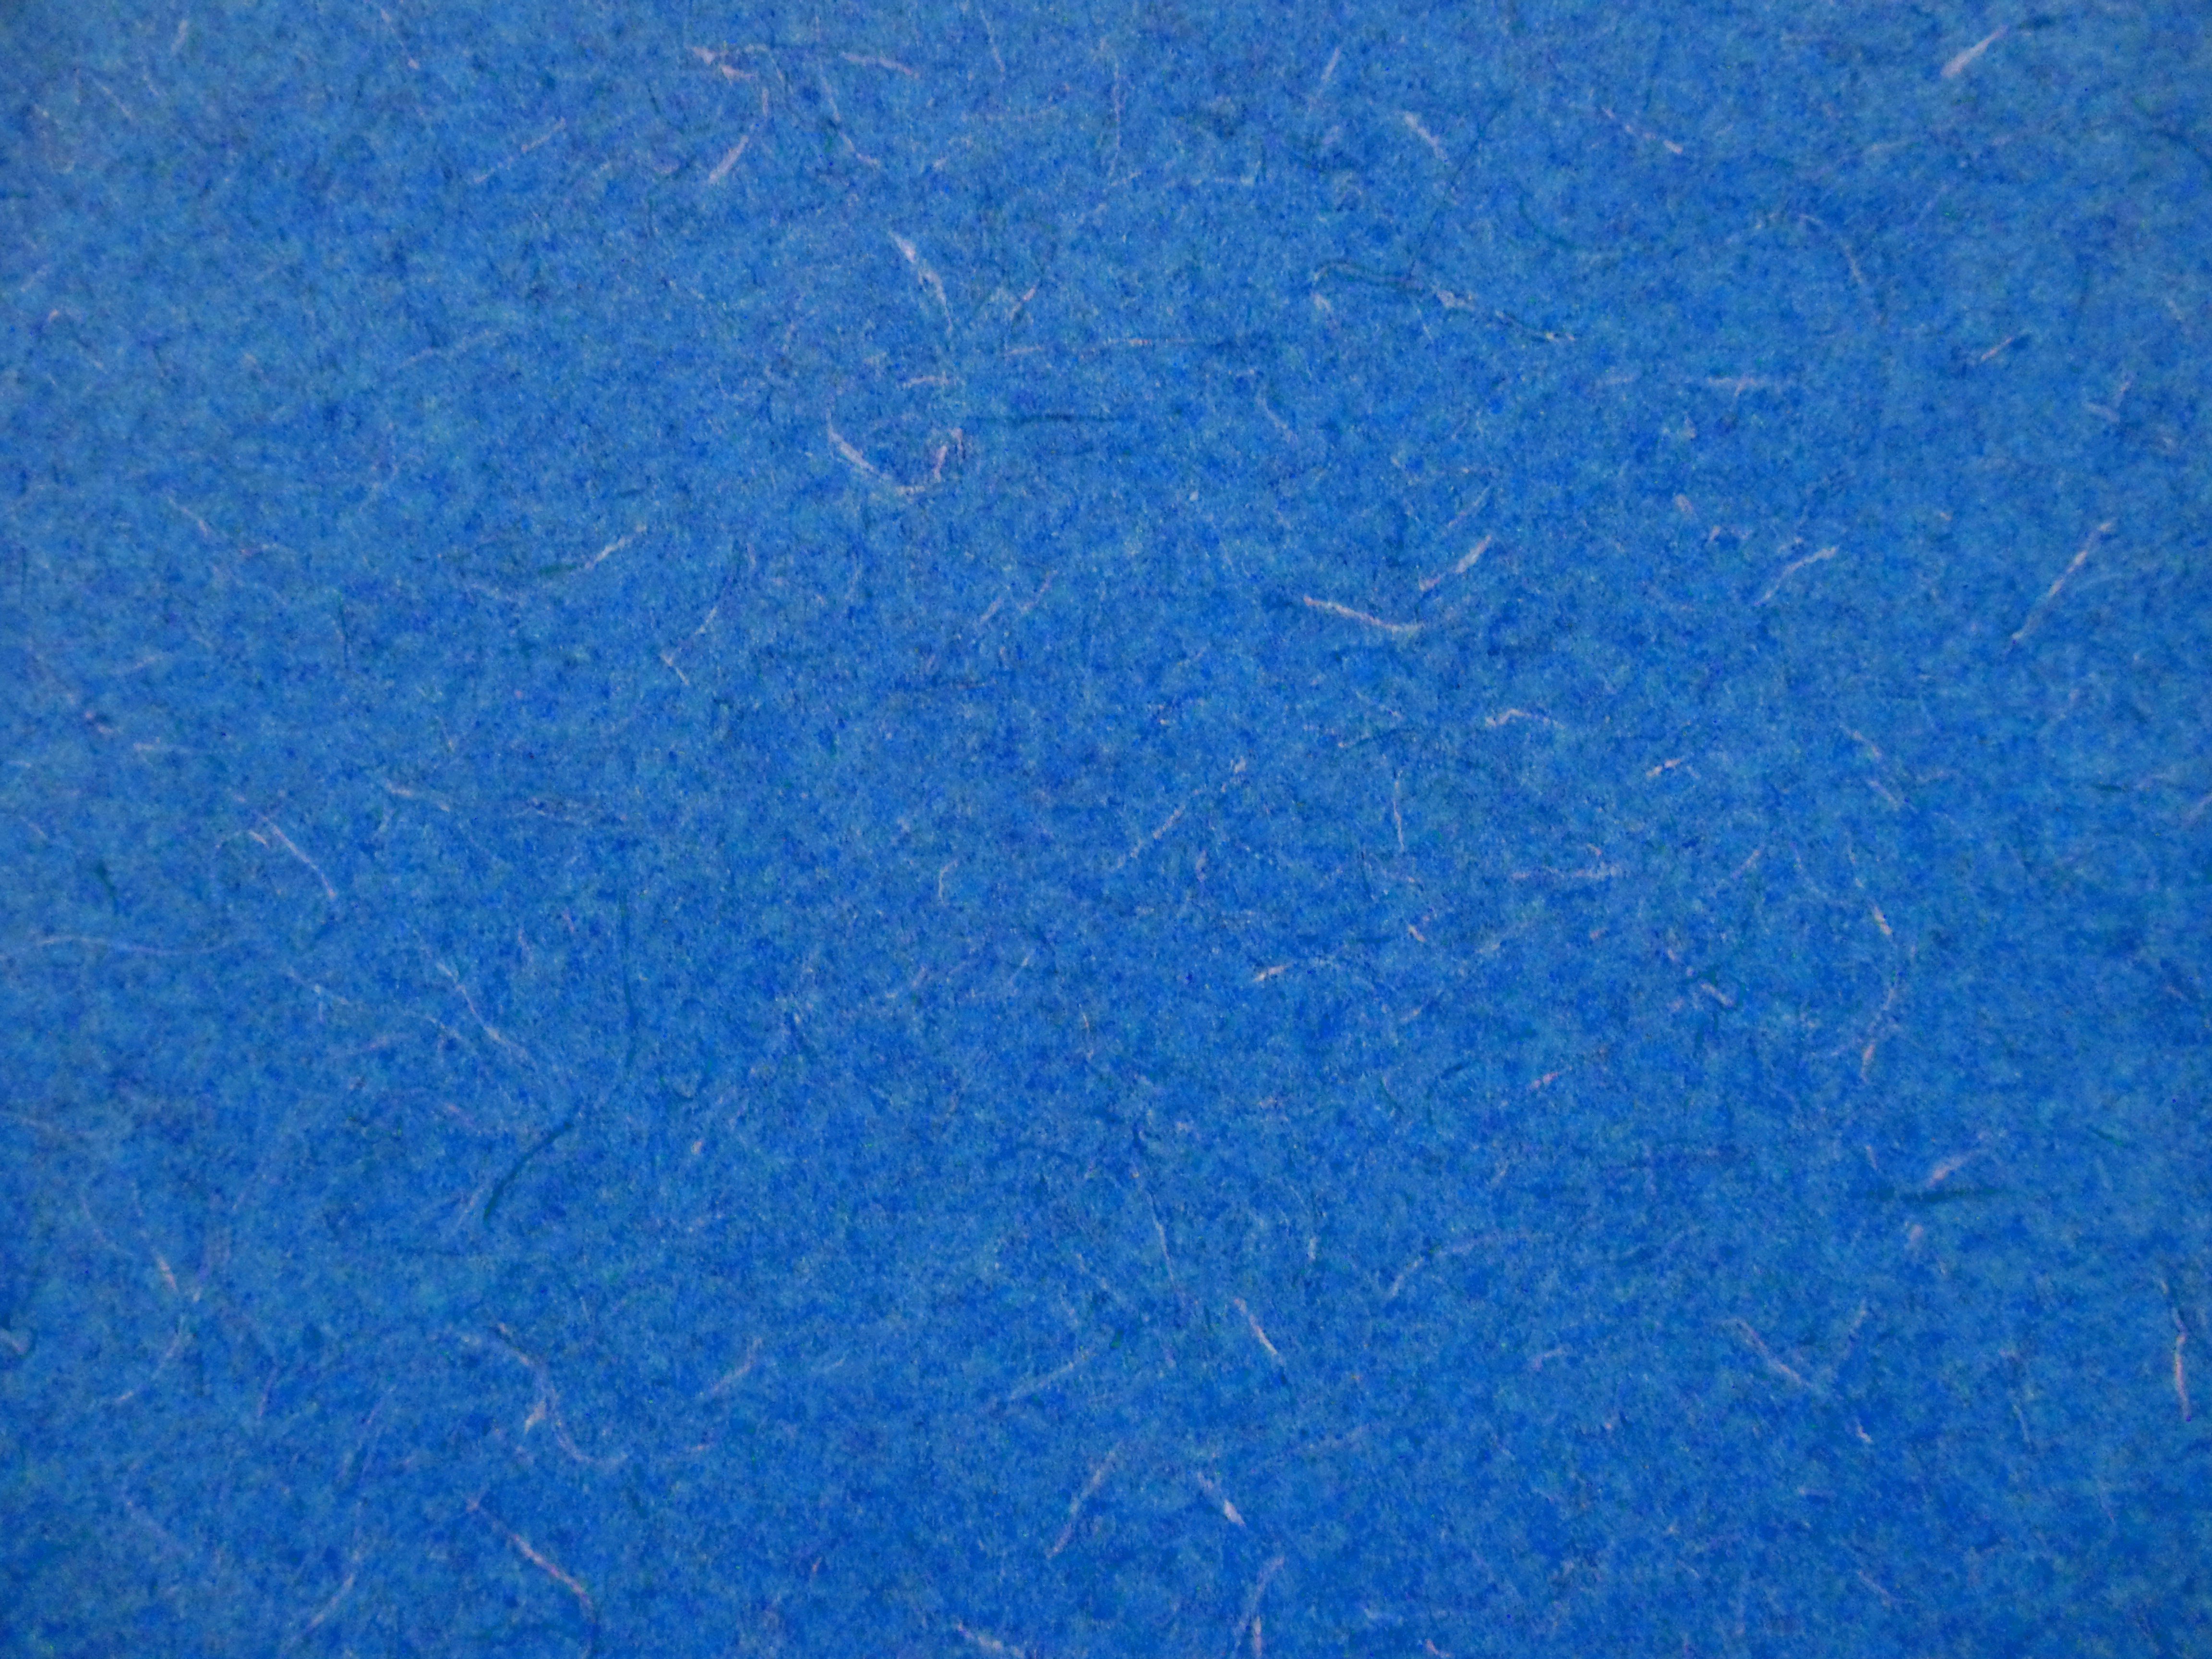
\includegraphics[width=\paperwidth,height=\paperheight]{chapters/images/background-texture-blue.jpg} %higherquality image but too big for overleaf
    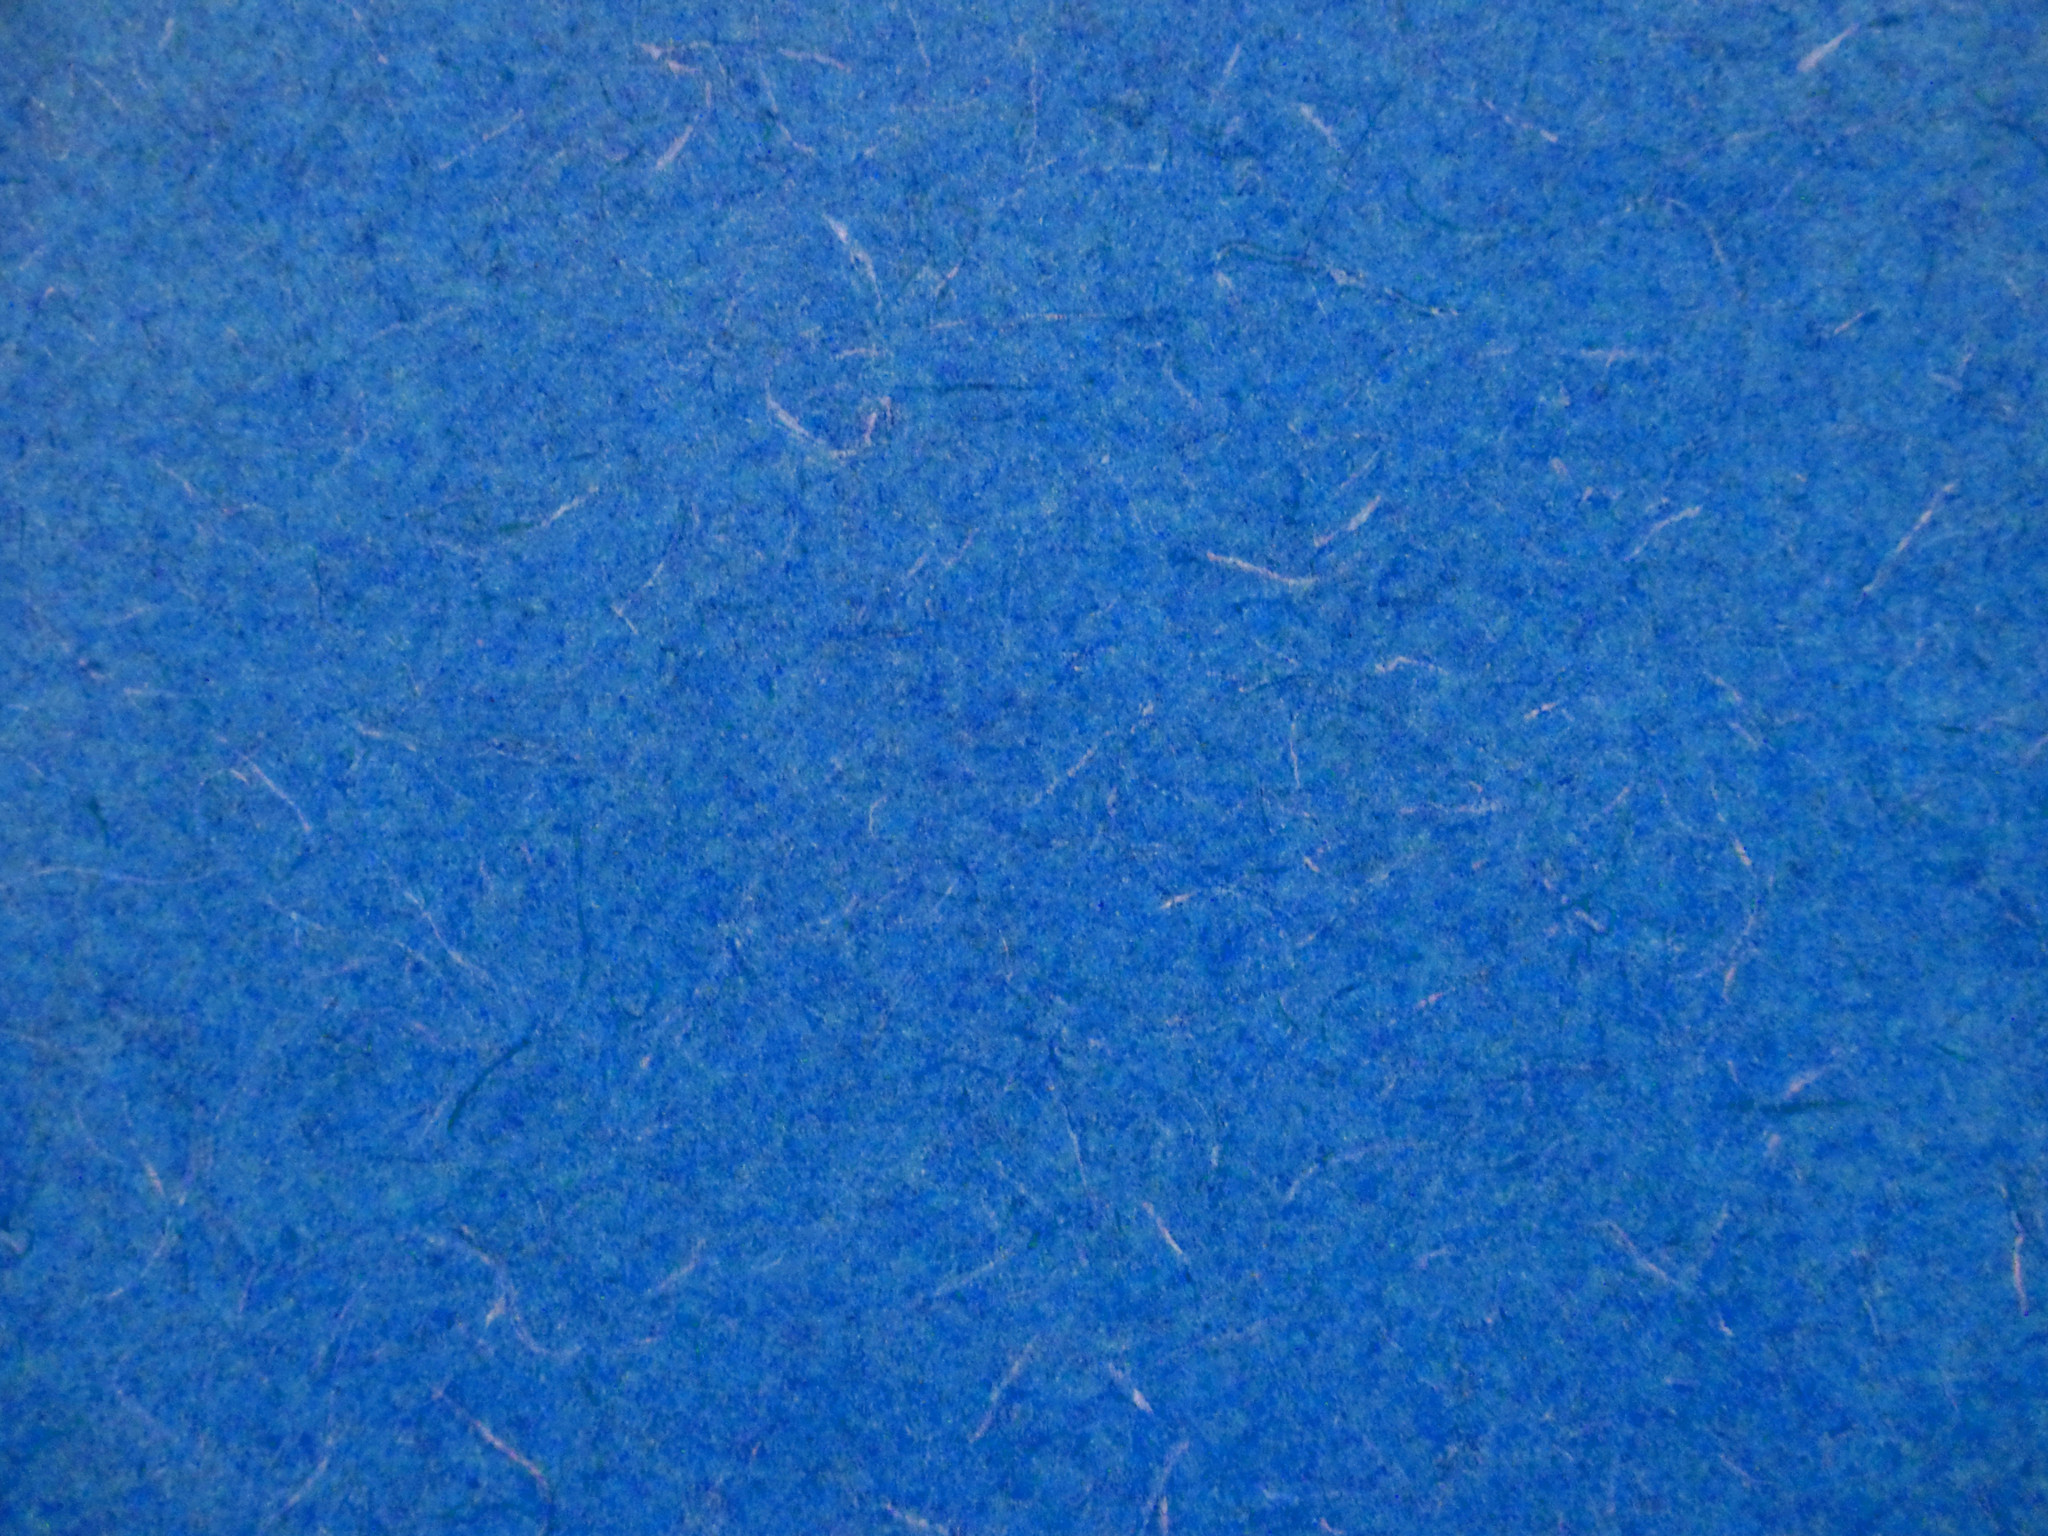
\includegraphics[width=\paperwidth,height=\paperheight]{chapters/images/background-texture-blue-reduced.jpg}
};
\sc
\begin{center}

\color{white}{
\Large Prostate Cancer \normalsize
\vspace{2cm}


I like puzzles. Any type of puzzle. I always have. If I see a puzzle or a problem I have to solve it. I think that is what makes cancer such a fascinating topic for me.

\vspace*{0.5cm}

Imagine you are given a jigsaw puzzle. Now instead of a few hundred pieces, there are several billion pieces. The picture on the box is not a picture of the puzzle inside the box,
it is just a somewhat similar image. Oh, and did I mention there are a whole bunch of pieces missing? and that many pieces are duplicated? Some pieces don't even belong in our box,
but come from a completely different puzzle. On top of that your little sister has spilled paint over some of the pieces so those can't be trusted to contribute to the image. And instead of one
single puzzle, the box contains several, they are all variations of the image on the box, but you have no idea how many different puzzles the box contains. Sound challenging? This is the problem we are solving whenever we sequence a cancer genome.

\vspace*{0.5cm}
\textbf{[Metaphor key]} \\
\textit{puzzle pieces} = sequence reads \\
\textit{picture on box} = reference genome \\
\textit{missing pieces} = hard-to-sequence areas \\
\textit{other puzzles} = contamination \\
\textit{painted pieces} = sequencing errors \\
\textit{multiple puzzles in box} = clonality
}

\end{center}
\end{minipage}
\end{center}



\newpage
\section{Use case 1: Prostate Cancer}

\epigraph{3in}{The time has come in America when the same kind of concentrated effort that split the atom and took man to the moon should be turned toward conquering this dread disease.}{President Richard Nixon}

On December 23, 1971, President Richard Nixon, buoyed by recent technical feats such as the moon landing, signed into law the National Cancer Act, thereby declaring a war on cancer. Today, more than 45 years later, that war is still being waged in full force. While great advancements have been made towards this goal, some of the initial optimism has been quelled by discoveries of the great complexity and heterogeneity underlying cancer.


\subsection{The Hallmarks of Cancer}

Tumor cells evolve from normal cells through the acquisition and accumulation of mutations. The human body has mechanisms in place to repair or dispose of damaged cells and to prevent runaway cell division, so in order for a tumour cell to survive and thrive it needs to acquire changes that provide it with advantages for proliferation and evasion of the cell's defense mechanisms. Evidence suggests this transformation from healthy cells into malignant cells follows a strikingly similar path across all different tumour types \cite{}. A cell's acquired abilities that drive tumour progression are know as the \emph{hallmarks of cancer} and consist of the following six characteristics:

\begin{itemize}
    \itemsep-0.5em
    \item self-sufficiency in growth signals
    \item insensitivity to anti-growth signals
    \item evasion of programmed cell death
    \item limitless replicative potential
    \item sustained angiogenesis
    \item tissue invasion and metastasis
\end{itemize}

Each of these steps overcomes one of the body's anti-cancer defense mechanisms. This evolution into malignancy is an almost darwinian process where the mutations acquired are random, but those cells that have gained mutations which are advantageous for survival will be able to replicate and thrive and accumulate further mutations. Distinguishing the mutations that impart a strategic advantage and thereby \emph{drive} a tumour's progression, from the often huge number of less harmful \emph{passenger} mutations accumulated over the lifetime of a cancer cell is no easy task. The optimal course of treatment for a patient often depends on the mutations present and how the cell functions are subsequently impacted by those mutations. %However, many different mutations may lead to the same disruptions of key pathways, therefore we must evaluate mutations not just at the DNA level but in the broader context of their functional impact on the cell's internal processes.



\subsection{Cancer's Complexities}

Determining the exact genetic sequence of healthy individuals is already quite a challenging endeavor; trying to extend this to cancer genomes takes this challenge to the extreme. There are several complexities present in cancer geneomes that make accurate determination of the genetic changes and their downstream impacts a difficult task. In the following sections we will discuss some of these complexities and explore the biological and informatics challenges they pose.

\subsubsection{The Bio}
\paragraph{Small variants} comprise the simplest class of mutations; those consisting of alterations of just a handful of bases, for instance the \emph{substitution}, \emph{deletion} or \emph{insertion} of one or more nucleotides.

The impact of such mutations depends on where in the genome they occur. Single nucleotide variants (SNVs) in exonic regions can range from having no effect on the resulting protein (silent), to changing an amino acid in the protein to a different amino acid (missense mutations), to changing a codon into a stop codon (nonsense mutation) which nearly always results in a nonfunctional protein. If this happens in a protein that is vital to the functioning of the cell this can have disastrous consequences <some examples of SNVs causing serious problems/phenotypes>

While variants within the coding sequence are most likely to have an impact on cell health, small variants \emph{outside} the coding sequence can also have drastic impact on health; for example, 70\% of melanomas exhibit a point mutation in one of two positions in the promoter region of TERT (Horn et al. 2013; Huang et al. 2013), suggesting such somatic point mutations in regulatory regions may play a role in tumorigenesis.

\paragraph{Structural variations (SVs)} are larger-scale mutations involving rearrangement of segments of DNA of more than roughly 50 bp. In some cases, these rearrangements can cause (parts of) two genes that are usually separated by some distance on the genome to come together to form new hybrid genes, which may be transcribed into fusion proteins, and which have a potentially disastrous effect on cell processes. The text book example of such a gene fusion is the so-called Philedelphia fusion frequently observed in leukemia \cite{TODO}. In this Philedephia chromosome, a translocation between chromosomes 9 and 22 leads to a fusion of the BCR and ABL1 genes. This fusion gene is expressed, and the aberrent fusion protein causes disruptions to key signalling pathways governing the cell cycle, causing the cells to divide uncontrollably and thereby drive tumor progression. Accurate detection of such structural variations is crucial, as they may serve as diagnostic markers \cite{nowell1960chromosome,nowell1961chromosome} or even therapeutic targets \cite{druker2001activity, druker2001efficacy}.

SVs often occur outside coding regions, but this does not diminish their potention for great impact, for instance by disruption of the regulatory mechanisms of tumour supressor genes or oncogenes \cite{TODO}. These types of SVs not involving coding regions directly, may only be detected through whole-genome sequencing.

%Numerous fusion genes have been found to play a role in tumorigenesis \cite{TODO},
%in prostate cancer the TMPRSS2-ERG fusion is present in roughly 40\% of tumours, \cite{TODO}

\paragraph{Clonality} refers to the phenomenon that cells in different physical areas in a tumour may be genetically very distinct. As a cell obtains a mutation that is beneficial to proliferation, it may instigate a new cluster, or \textit{clone}, of genetically similar cells while in other areas of the tumour cells may follow a different evolutionary path and create genetically different subclones. When sequencing a tumour, DNA from different cells -and thus potentially very different genomes- is mixed together and sequenced as one. Reconstructing the different clonal genomes from this data is immensely challenging.

\paragraph{Further complexities} in the analysis of cancer genomes include the temporally evolving nature of tumours; performing the same sequencing experiment on the same tumour at different points in time will often yield a very different picture as the composition of the tumour and the acquired mutations will have changed. This further complicates the process of comparing different samples and elucidating key characteristics that have the potential to aid in the diagnosis and treatment of patients. Furthermore, studies in epigenetics have shown that tumorigenesis is not solely driven by mutations in nucleotide sequence, but secondary alterations such as DNA methylation may have an equal if not greater impact \cite{TODO}.

\subsubsection{The Informatics}

All these complexities in the biology of cancer gemomes translate to complexities of the downstream informatics analysis pipelines.


We know that changes in sequence and structure of DNA contributes to cancer development. But how do we describe these properties? Any two healthy individuals differ greatly in their DNA sequence; it's what makes us us. How to denote these differences is a non-trivial problem, as is determining which of these differences are just part of the natural variation between individuals and which are ones detrimental to our health and functioning.

If you were asked to describe the differences between two Shakespeare plays, how would you go about it? They are made up of the same alphabet, and share many of the same words and even whole sentences, but to list the differences between them can be done in many ways. You could number the words in both books and take note of the ones that are different in each position, but then if you were to take two identical sentences and prefix one with a single extra word, all positions would end up being flagged as different while clearly these sentences are nearly identical. And ..

<note: ditch the book analogy? example shakespearean sentence to illustrate? >

poor concordance between variant callers: https://genomemedicine.biomedcentral.com/articles/10.1186/gm432


Currently variations in DNA are described relative to a \emph{reference genome}; a sequence intended to represent the \emph{average} human genome, which was constructed by taking the most frequently observed nucleotide at any given  position in the genome
<discuss some drawbacks/things to realize: based on relatively small set of samples, not optimally diverse set of individuals>

\begin{comment}
As we have seen, the choice of software can impact downstream analysis, and variant calling is no exception. Different aligners employ different mapping strategies, which leads to different variant calls for the same observed sequence depending on the choice of algorithm, complicating variant comparisons between studies \cite{zook2014integrating}. While there do exist tools to canonicalise some of these differing representations \cite{vcflib}, complex variants remain that do not have a single obvious standard form (Figure \ref{fig:variant-multiple-representations}).
But even for the simpler cases, there is not always a clear consensus on how to standardise representation. Consider for instance the case where an adenine nucleotide has been inserted, transforming the sequence \verb+TAAG+ to \verb+TAAAG+. Do we describe the insertion to have happened at position 1 (after the \verb+T+), position 2 (between the two \verb+A+s), or at position 3 (before the \verb+G+)? While this particular case is easily solved by agreeing on a convention of either left-aligning or right-aligning these variants, such community agreement does not currently exist, with most next-generation analysis tools opting for left-alignment, while certain variant databases such as HGVS [TODO cite] still recommend (but do not enforce) alignment to the position nearest the 3\` end of the gene \cite{hgvs-position}, which translates to right-alignment in genomic coordinates for reverse strand genes. Furthermore, once variants have been submitted to online databases, information about surrounding variants observed in the same sample is often not kept, making it impossible to resolve equivalency of variant representations going forward.
\end{comment}


\begin{figure}[h!]
    \centering
    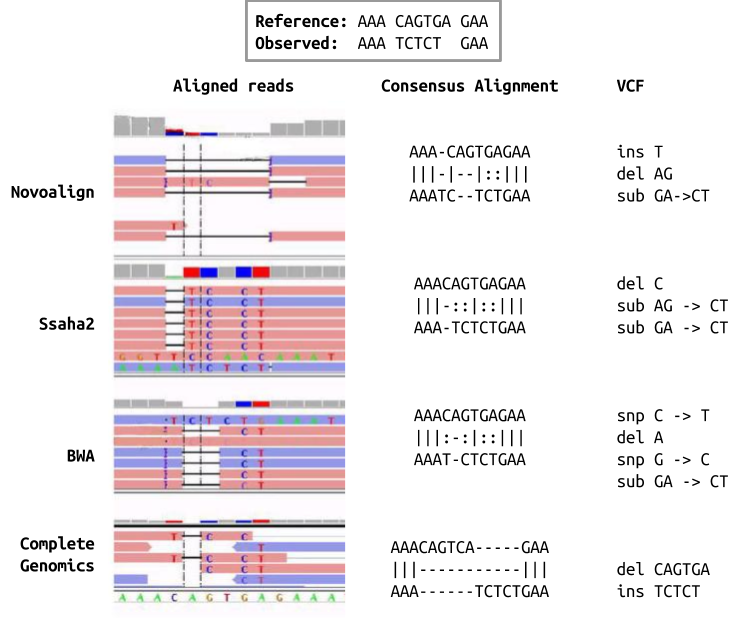
\includegraphics[width=400pt]{chapters/images/variant-representation-all.png}
    \begin{comment}
        image in google drive https://docs.google.com/drawings/d/1WWmzW6uWtJ7HZ5WVgtg_oAMA_3E_569M4Ikjz4Ecjic/edit
    \end{comment}
    \caption{Complex variants can be represented in multiple ways. Four different aligners (Novoalign, Ssaha2, BWA, Complete Genomics) treat the same variant in vastly different ways, which leads to such differing sets of variant descriptions in the VCF files that it is no longer apparent that these variants in fact describe the same observed sequence.}
    \label{fig:variant-multiple-representations}
\end{figure}


<not to mention sequencing errors, at rate of abt x/100, sequencing depth helps but tradeoff with cost>

sources of mismatch with reference genome \\
- real mutation \\
- wrong base call \\
- wrong mapping/variant call \\


<repetitive regions>

The result of all of this is that different variant calling tools will produce different sets of variants given the exact same input dataset and reference genome, and it is hard to know who does a better job, if their respective papers are to be believed each one of them far outstrips all the others. But as with everything in life, the truth lies somewhere in the middle. Each of the variant callers has its strengths and weaknesses, some may very accurate in calling one type of variant but have  more difficulty with others. Some are very accurate in healthy genomes but less so in highly mutated genomes or vice versa. One possible solution is to run a set of variant callers

\paragraph{Structural variations}
<very very poor overlap between different methods>

<hard to resolve exact location of junctions>

<chainfinder>
\paragraph{Clonality}
\paragraph{Temporal Evolution}
\paragraph{Epigenetics}



\newpage
\thispagestyle{empty}
\begin{center}
\vspace{2cm}
\begin{minipage}{5in}
\tikz[remember picture,overlay]
\node[opacity=0.8,inner sep=0pt] at (current page.center){
    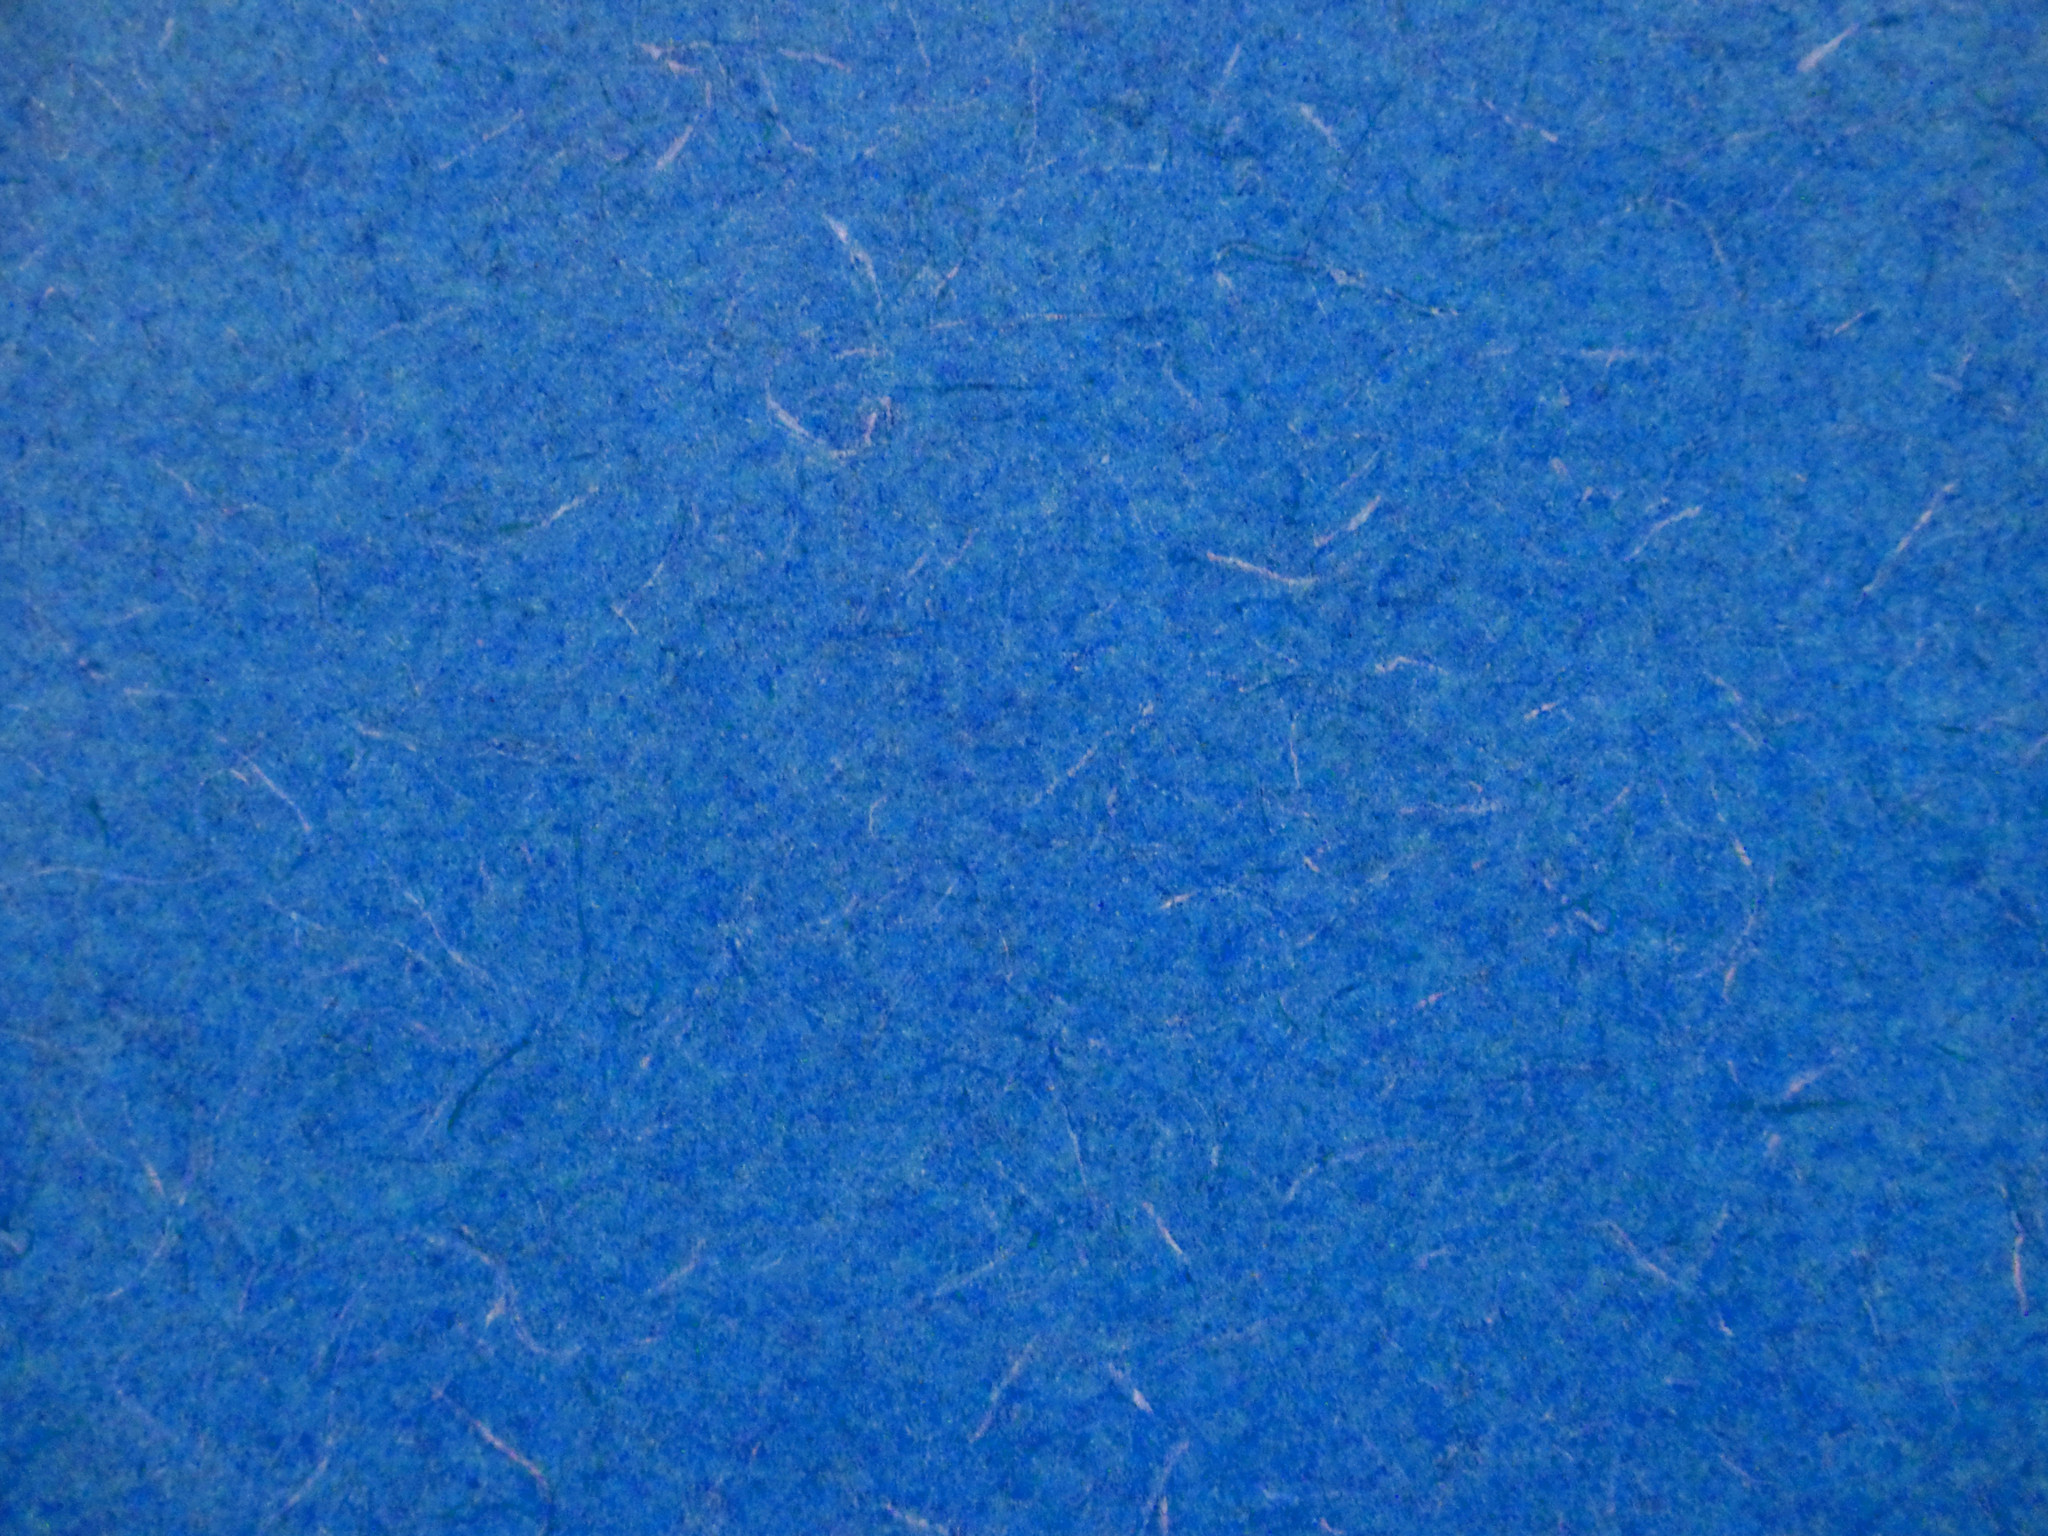
\includegraphics[width=\paperwidth,height=\paperheight]{chapters/images/background-texture-blue-reduced.jpg}
};
\sc
\begin{center}

\color{white}{
\Large The Human Microbiome \normalsize
\vspace{2cm}

When Dutch inventor and scientist Antonie van Leeuwenhoek first turned his microscope to a drop of rain water and discovered within a wealth of microscopic life which he termed \textit{animalcules}, a whole new world of knowledge opened up. Soon after, it was discovered that while these organisms might be microscopic in size, their impact on human lives was enormous, causing food to spoil and disease to spread. Through the study of these micro-organisms, scientists were able to develop methods for enhanced food preservation and eventually also new treatments and vaccines for a whole range of illnesses.

Cost of sequencing has now dropped enough that it has become feasible to sequence not only a patient's own DNA, but also the DNA of their microbiome to make a diagnosis or to determine the best treatment option.




\vspace*{2cm}
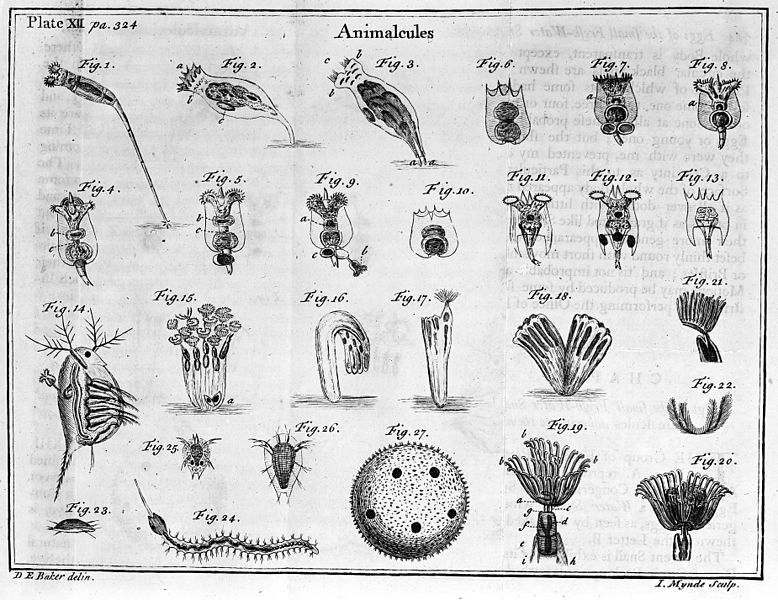
\includegraphics[scale=2]{chapters/images/mycrobiota/animalcules2.png}

}

\end{center}
\end{minipage}
\end{center}

\newpage


\section{Use case 2: Microbiota}

\begin{comment}

overview of reading materials about the human microbiome

http://www.richardsprague.com/note/2017/10/16/best-academic-papers-about-the-microbiome/

informal history of microbiology: https://www.bioexplorer.net/history_of_biology/microbiology/
\end{comment}

\subsection{The Bio}
first complete bacterial genomes published in 1995  \cite{land2015insights}

16S rRNA

whole genome shotgun

\subsection{The Informatics}


\begin{comment}
history of microbiolgy: https://courses.lumenlearning.com/boundless-microbiology/chapter/introduction-to-microbiology/

<WGS reveals changes outside coding regions, such as one affecting regulation of genes are of importance, and can reveal large scale changes (SVs), fusion genes>

<epigenetics>

<potential of developing treatments from all this knowledge>

sources:
- Hallmarks of cancer: the next generation [@hanahan2011hallmarks]
- Chromosome aberrations in solid tumors [@albertson2003chromosome]

~~~
low-resolution methods:
- fluorescent in sit hybridisation FISH [Pinkel et al 1988, Thompon and Gray, 1993]
- chromosome painting [Jauch et al, 1992]
- spectral karyotyping [Schrock et al 1996]
- comparative genome hybridisation CGH [Kallioneimi 1992]

- arrays

high-throughput:
 - LOH [@hampton1996simultaneous]
 - GWAS

 - 2003 still infeasible to sequence entire tumor genome, so
   ESP (end sequencing profiling) used [Volik et al 2003]
       (- BAC library from tumor, sequence ends, map to reference)
    → reconstruction from ESP data [Rapael et al 2003]

now: WGS
- NGS: DNA short reads
- NGS: RNA Seq
- NGS: Paired end mapping [@korbel2007paired]
- limitations of current methods
~~~

advanced in cancer research specifically from next generation methods: [@meyerson2010advances]

\end{comment}







\begin{comment}

types of SVs: standard, complex, chromothripsis [@stephens2011massive]

- well-known examples
    - TMPRSS ERG
    - ABL gene on chr9, chronic myeloid leukema, translocation between chr9 and 22,
       changes regulation, promotor becomes promotor of BCR gene on chr22
      [Heisterkamp et al 1983]

#### usefulness in biomarker and treatment development

- Gleevec, targeting BCR-ABL fusion gene [@druker2001efficacy]
- Herceptin, targeting ERBB2 amplification [@kauraniemi2004effects]


#### SV Tools and databases

~~~
- catalogued in Mitleman database [Mitelman 2003]
- COSMIC
- ..
~~~

## Clonality

## Temporal evolution

## etc..
~~~
<Informatics/analysis methods>
 - History of methodologies (gwas, ..)
 - NGS: Huge datasets, excel and manual analyses no longer suffice
 - Cancer: Germline correction, drivers vs passengers

<Limitations of current methods>
 - imperfect data
 - disagreements and biases per lab/informatics technique

<Challenges in tumour genome reconstruction>
→ explain in biology section, here describe why that complicates things

 - Normal Contamination
 - Clonality detection
 - Event Chains detection
 - Temporal evolution detection


\end{comment}

\section{Scope of this Thesis}
Bioinformatics is a vital part of many fields of research. While these may differ greatly in the biology involved, many of the bioinformatics concepts are shared among them. In \hyperref[chapter:general]{Chapter \ref{chapter:general}} we discuss several such widely-applicatble bioinformatics projects. Galaxy for reproducible analysis workflows, iReport for results reporting withing Galaxy. (Circos? myFAIR?)



\bibliographystyle{ieeetr}
\bibliography{references}

\begin{justify}
\begin{savequote}[75mm]
Nulla facilisi. In vel sem. Morbi id urna in diam dignissim feugiat. Proin molestie tortor eu velit. Aliquam erat volutpat. Nullam ultrices, diam tempus vulputate egestas, eros pede varius leo.
\qauthor{Quoteauthor Lastname}
\end{savequote}

\chapter{Bioinformatics Tools}
\label{chapter:general}
\setcounter{figure}{-1}
\setcounter{table}{-1}
\setcounter{section}{-1}
%\setcounter{enumiv}{-1}
\setcounter{NAT@ctr}{-1}

\begin{verbatim}
iReport, Circos?, myFAIR?, Galaxy2018update? (I am co-author and technically everybody is
shared first on that? would fit nicely with the overall story as every other paper connects
to Galaxy.)
- Training paper in its own section or add it here?
\end{verbatim}

Bioinformatics plays a role in a wide range of research fields. While the biology might be vastly different, many of the underlying bioinformatics concepts are shared and may be reused regardless of the scientific application. This chapter covers a number of such generic bioinformatics applications. The Galaxy project provides a graphical user interface to commandline unix tools. iReport provides a generic reporting tool within the Galaxy framework. Circos offers visualisation for high-dementional data. The myFAIR application is designed to integrate the Galaxy platform to FAIR data management applications, to further facilitate reproducible research.

  %reset references counter
\setcounter{NAT@ctr}{-1}
\cleartorightpage
\chapter*{}
\phantomsection\addcontentsline{toc}{section}{Galaxy: the 2018 update}

\begin{figure}[t!]
\centering

\includegraphics[height=10em]{frontmatter/images/chapter-header-galaxy.png}
\end{figure}
\vspace{-4cm}

\begin{changemargin}{0cm}{2cm}
\articletitle{The Galaxy platform for accessible, reproducible and collaborative biomedical analyses: 2018 update}
\end{changemargin}


Enis Afgan\textsuperscript{\ref{affil:hopkins},*},
Dannon Baker\textsuperscript{\ref{affil:hopkins}},
Bérénice Batut\textsuperscript{\ref{affil:freiburg},*},
Marius van den Beek\textsuperscript{\ref{affil:curie},*},
Dave Bouvier\textsuperscript{\ref{affil:pennstate},*},
Martin Čech\textsuperscript{\ref{affil:pennstate},*},
John Chilton\textsuperscript{\ref{affil:pennstate},*},
Dave Clements\textsuperscript{\ref{affil:hopkins},*},
Nate Coraor\textsuperscript{\ref{affil:pennstate},*},
Björn Grüning\textsuperscript{\ref{affil:freiburg},*},
Aysam Guerler\textsuperscript{\ref{affil:hopkins},*},
Jennifer Hillman-Jackson\textsuperscript{\ref{affil:pennstate},*},
Saskia Hiltemann\textsuperscript{\ref{affil:emc},*},
Vahid Jalili\textsuperscript{\ref{affil:oregon},*},
Helena Rasche\textsuperscript{\ref{affil:freiburg},*},
Nicola Soranzo\textsuperscript{\ref{affil:earlham}},
Jeremy Goecks\textsuperscript{\ref{affil:oregon},*},
James Taylor\textsuperscript{\ref{affil:hopkins},*},
Anton Nekrutenko\textsuperscript{\ref{affil:pennstate},*},
Daniel Blankenberg\textsuperscript{\ref{affil:cleveland},*}

* The authors wish it to be known that, in their opinion, all authors should be regarded as Joint First Authors.

\textbf{Published in:} \emph{Nucleic Acids Research}, Volume 46, Issue W1, 2 July 2018, Pages W537–W544,  \\
DOI: \url{https://doi.org/10.1093/nar/gky379}

\small
\begin{enumerate}
\itemsep-0.5em
\item Department of Biology, Johns Hopkins University, Baltimore MD USA.\label{affil:hopkins}
\item Department of Comuter Science, Albert-Ludwigs-University, Freiburg, Germany.\label{affil:freiburg}
\item Institut Curie, PSL Research University, Paris, France.\label{affil:curie}
\item Department of Biochemistry and Molecular Biology, Penn State University, University Park, PA, USA.\label{affil:pennstate}
\item Center for Biological Systems Analysis (ZBSA), University of Freiburg, Freiburg, Germany.\label{affil:freiburg2}
\item Department of Pathology, Erasmus Medical Centre, Rotterdam, The Netherlands.\label{affil:emc}
\item Department of Biomedical Engineering, Oregon Health and Science University, OR, USA.\label{affil:oregon}
\item Earlham Institute, Norwich Research Park, Norwich, United Kingdom.\label{affil:earlham}
\item Genomic Medicine Institute, Lerner Research Institute, Cleveland Clinic, Cleveland, OH, USA.\label{affil:cleveland}
\end{enumerate}
\normalsize


\section*{Abstract}
Galaxy (homepage: \url{https://galaxyproject.org}, main public server: \url{https://usegalaxy.org}) is a web-based scientific analysis platform used by tens of thousands of scientists across the world to analyze large biomedical datasets such as those found in genomics, proteomics, metabolomics, and imaging. Started in 2005, Galaxy continues to focus on three key challenges of data-driven biomedical science: making analyses accessible to all researchers, ensuring analyses are completely reproducible, and making it simple to communicate analyses so that they can be reused and extended. During the last two years, the Galaxy team and the open-source community around Galaxy have made substantial improvements to Galaxy’s core framework, user interface, tools, and training materials. Framework and user interface improvements now enable Galaxy to be used for analyzing tens of thousands of datasets, and more than 5,500 tools are now available from the Galaxy ToolShed. The Galaxy community has led an effort to create numerous high-quality tutorials focused on common types of genomic analyses. The Galaxy developer and user communities continue to grow and be integral to Galaxy’s development. The number of Galaxy public servers, developers contributing to the Galaxy framework and its tools, and users of the main Galaxy server have all increased substantially.


\section*{Introduction}
Advances in biomedicine and biology increasingly rely on analysis of large datasets. Started in 2005, the Galaxy Project (\url{https://galaxyproject.org})~\cite{giardine2005galaxy,blankenberg2007framework,afgan2016galaxy} maintains a focus on enabling data-driven biomedical science by pursuing three goals: (a) accessible data analysis serving all scientists regardless of their informatics expertise and tool developers seeking a wider audience and broad integration of their tools; (b) reproducible analyses regardless of the particular platform; and (c) transparent communication of analyses, which in turn enables reuse and extension of analyses across communities of practice. The Galaxy Project consists of four complementary components:

\begin{enumerate}
\item The main public Galaxy server (\url{https://usegalaxy.org}) — this server is the subject of this article and has been online since 2007. It features a rich toolset for large-scale genomics analyses, terabytes of public data for use, and hundreds of shared analysis histories, workflows, and interactive publication supplements. This server has more than 124,000 registered users whom run \~245,000 analysis jobs each month.

\item The Galaxy framework and software ecosystem (\url{https://github.com/galaxyproject}) — an open-source software package that anyone can use to run a Galaxy server on any Unix-based operating system. The Galaxy ecosystem includes a software development kit (SDK) for Galaxy tool development, API language bindings for multiple programming languages, software for scripting Galaxy interactions, and tools for automating setup and deployment of Galaxy and its plugins such as tools and visualizations.

\item The Galaxy ToolShed (\url{https://toolshed.g2.bx.psu.edu/}) — a community-driven resource for the dissemination of Galaxy tools, workflows, and visualizations. This server functions as an “AppStore” for Galaxy servers where developers and Galaxy admins can host, share, and install Galaxy tools, workflows, and visualizations.

\item The Galaxy Community (\url{https://galaxyproject.org/community/}) — distinct and complementary subcommunities make key contributions to all aspects of the Project. These subcommunities address the needs and desires of every category of stakeholder including users, administrators, developers, resource providers, and educators.
\end{enumerate}

Galaxy has served hundreds of thousands of users, been used in more than 5,700 scientific publications, and provided 500+ developers with a framework provisioning accessible, transparent, and reproducible data analysis (\url{https://galaxyproject.org/galaxy-project/statistics/}). Many instances of the framework have been installed, including Galaxy Main (\url{https://usegalaxy.org}) and over 99 publicly accessible servers (\url{https://galaxyproject.org/public-galaxy-servers/}), serving biomedical and other domain-specific research. Significant growth has occurred across all sectors of the Galaxy Project within the past two years (\hyperref[fig:growth]{Fig.~\ref{fig:growth}}).


\begin{figure}[ht!]
\centering
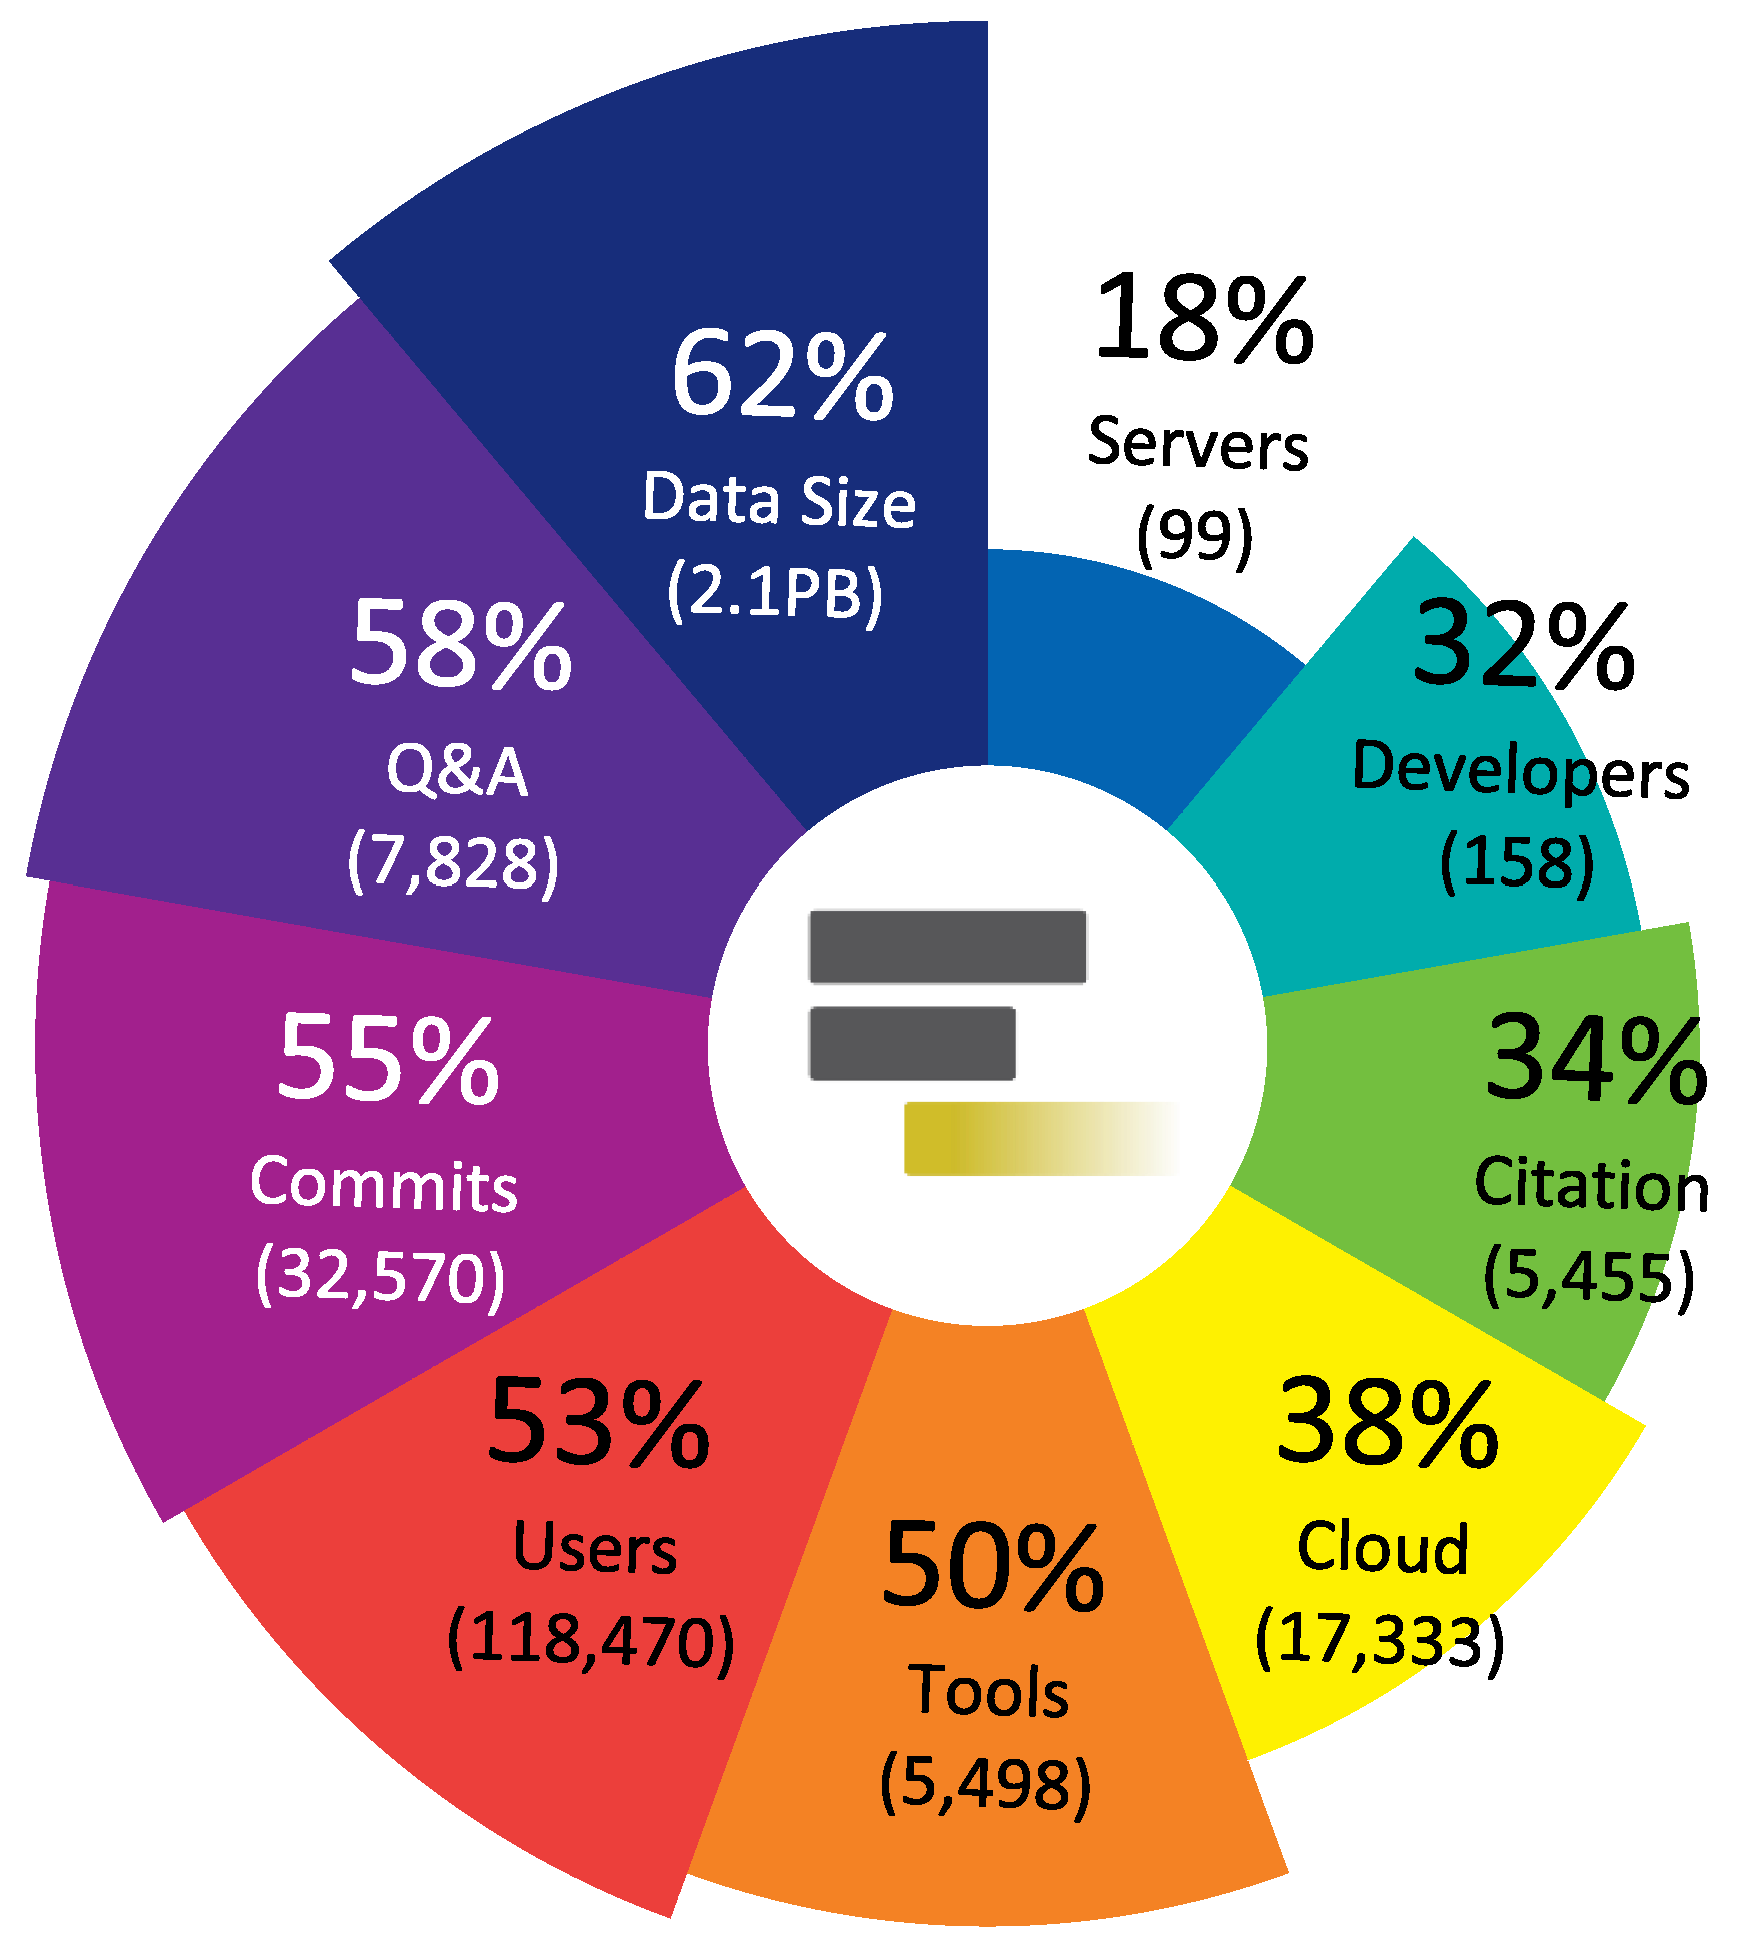
\includegraphics[]{chapters/images/galaxy/galaxy-growth.png}
\caption{Circular barplot illustrating recent growth of the Galaxy Project across several independent facets. In the past two years, usage of the main public Galaxy server has increased 60\%, the number of tools and supported versions has increased 53\%, and the amount of data analyzed on the main server has increased 72\%. A growing number of public instances (18\% increase) and cloud-based Galaxies (38\% increase) provide researchers with a wider range of options for scalability and application domains. Additionally, more developers (45\% increase with 63\% more commits to the codebase) contributed to the Galaxy framework and software ecosystem. Question and answer activity on the Galaxy Biostars forum increased 68\%.}
\label{fig:growth}
\end{figure}

\section*{New Features}
\subsection*{Scalability}
Scalability is amongst the most significant challenges that Galaxy faces as the size and number of biomedical and especially genomics datasets continues to grow. For instance, single-cell RNA-seq experiments routinely generate hundreds or thousands of primary datasets. As a web-based application, Galaxy must scale both in its web-based interface and on its backend server and do so in a multiuser environment.

\paragraph*{User interface scalability} enables scientists to use the Galaxy web interface to analyze many datasets, apply (collective) operations on them, and design pipelines to analyze them. Galaxy implements a variety of features to facilitate analyzing large numbers of datasets, including workflows and collections. Our recent optimizations of the user interface (UI) yielded a significant improvement to frontend scalability. We benchmarked the optimizations by replicating an experiment conducted on single Hematopoietic stem cells and multipotent progenitors~\cite{yang2016single} to quantify the expression of 64,000 transcripts, which generates 11,872 history items. Galaxy ran this proof of concept experiment seamlessly using existing standard tools, whereas earlier versions of Galaxy would not have been able to support this analysis.

\paragraph*{Server scalability} refers to the Galaxy’s ability to execute many data analysis/manipulation tasks for many users. This is achieved by advantageously utilizing a range of available computing resources. The Galaxy framework runs on various platforms, from a standard laptop to institutional clusters and cloud-based platforms. Galaxy is highly versatile in its ability to deploy jobs (atomic units of work), as it can leverage a multitude of workload managers including Slurm~\cite{yoo2003slurm}, HTCondor~\cite{thain2005distributed}, Apache Mesos~\cite{hindman2011mesos}, and Kubernetes (\url{https://kubernetes.io}), among others, in addition to a built-in lightweight job running system. Recent enhancements to Galaxy’s job management include dynamic job destination assignment (which facilitate automatic job parameter-specific resource selection), delay in job queuing (e.g., for workflows), automatic job re-submission (e.g., on job failure due to a temporary cluster error), and means of implementing fair-share prioritization schemes. These features are being used on Galaxy Main (\hyperref[fig:setup]{Fig.~\ref{fig:setup}}) to leverage cloud computing resources for better job throughput. Specifically, Galaxy Main is now configured to take advantage of the XSEDE infrastructure~\cite{towns2014xsede} that includes Bridges and Stampede resources as well as the Jetstream cloud~\cite{stewart2015jetstream}. The benefits of using these resources include the ability to run larger jobs, as shown in \hyperref[fig:infra]{Figure~\ref{fig:infra}}. Additionally, use of these resources has enabled new types of analysis to be enabled on Main. Notably, this includes Galaxy Interactive Environments through to the ability to use containerization technologies and provide sufficient isolation of individual jobs from other processes running on the same underlying compute infrastructure.

\begin{figure}[t!]
\centering
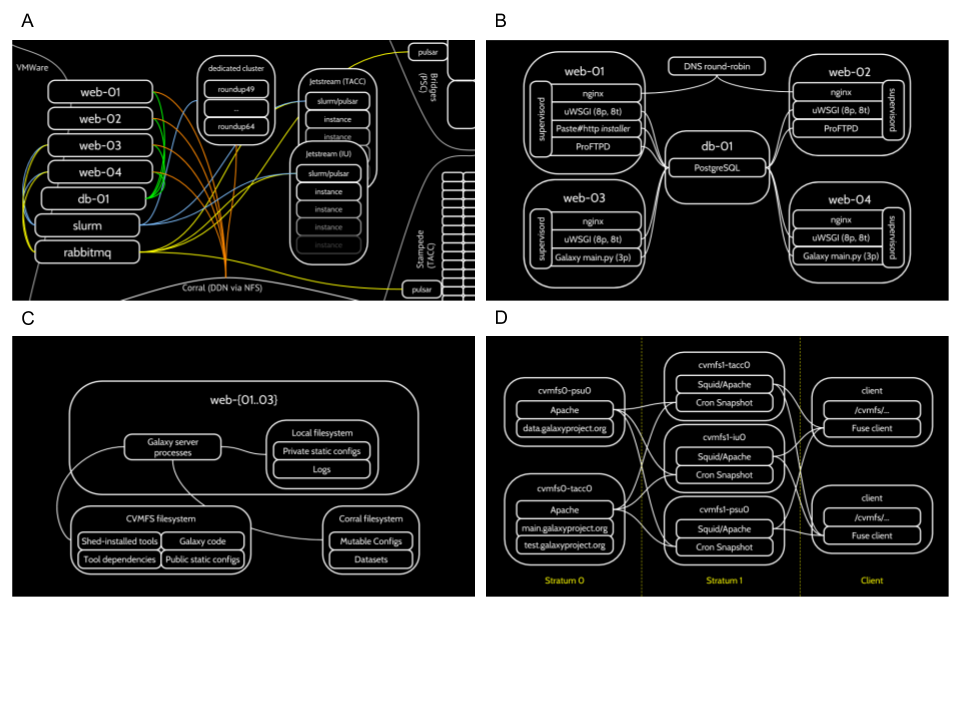
\includegraphics[width=\textwidth]{chapters/images/galaxy/setup.png}
\caption{Schematic of servers and services in use at Galaxy Main. (A) A global overview of Galaxy Main resources. (B) Multiple frontend servers serve Galaxy content to users by utilizing round-robin load balancing. (C) Layout of data schemes used by Galaxy Main is optimized for application speed, concurrent access, and versioned content. (D) CVMFS infrastructure hosted by the Galaxy Project that is used at Main and available for access to any other Galaxy instance.}
\label{fig:setup}
\end{figure}

\begin{figure}[t!]
\centering
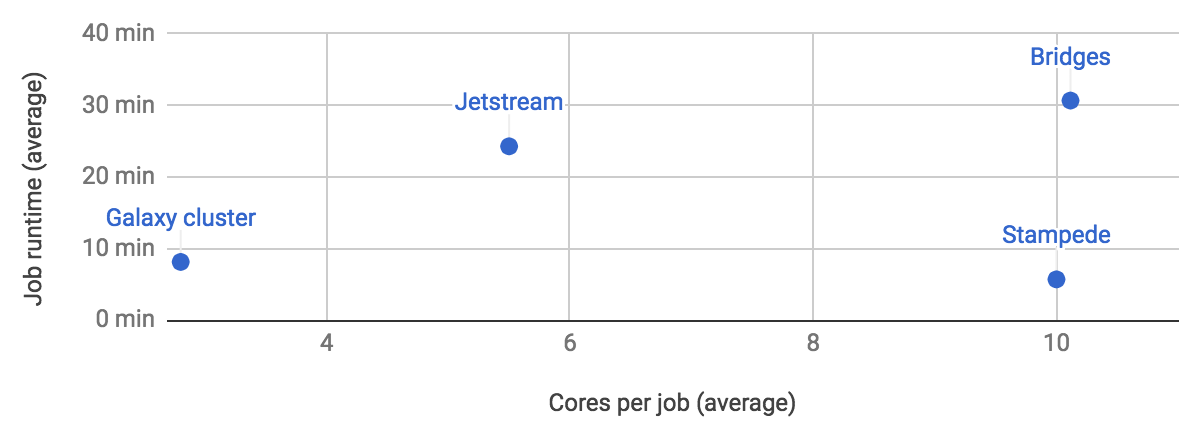
\includegraphics[width=\textwidth]{chapters/images/galaxy/infra.png}
\caption{Enabling automated selection and use of specialized national cyberinfrastructure compute resources from Galaxy Main enhances user-experience. It is now possible to run jobs that are up to an order of magnitude larger than before by using Bridges and Stampede. New types of jobs, such as interactive environments (see Advances in tools section), that require execution isolation due to security concerns are enabled by utilizing virtualization facilitated by the Jetstream cloud. Consequently, it is possible to concurrently run more jobs due to the increase in processing capacity.}
\label{fig:infra}
\end{figure}

A complete Galaxy server with a full repertoire of tools and reference data can be run on major cloud platforms. These servers are launched independently by users, and come pre-configured with hundreds of tools and reasonable default settings typical of a production server. Notably, launched instances do not have usage quotas and can be customized to install any desired tool. We have designed a cloud-agnostic approach for leveraging these resources by developing the abstraction library CloudBridge~\cite{goonasekera2016cloudbridge} and a new CloudLaunch application. These two solutions make it possible to launch Galaxy instances across a variety of cloud providers while reducing the requirement to build and maintain cloud-specific resources (e.g., machine images, file systems). There are now ten different flavors of Galaxy available for launching on major clouds including Amazon Web Services, Jetstream, and Microsoft Azure (\url{https://launch.usegalaxy.org}).

\subsection*{Advances in tools}
The Galaxy ToolShed~\cite{blankenberg2014dissemination} assumes the role of an AppStore for Galaxy instances by hosting thousands of tools. The ToolShed improves tool availability, deployment, and portability across Galaxy servers and computing environments.

\paragraph*{Updated tool suite} Over the last two years, we have expanded both the quantity and quality of the tools available on the Galaxy Toolshed. As of April 2018, the ToolShed hosts 5,628 tools, which shows 53\% growth since 2016, and approximately 2,000 repositories had at least one new update. Examples of new tools include: GEMINI for exploring genetic variation~\cite{paila2013gemini}; mothur for analyzing rRNA gene sequences~\cite{schloss2009introducing}; QIIME for quantitative microbiome analysis from raw DNA sequencing data~\cite{caporaso2010qiime}; deepTools for explorative analysis of deeply sequence data~\cite{ramirez2014deeptools,ramirez2016deeptools2}; HiCexplorer~\cite{ramirez2018high} for analysis and visualization of Hi-C data; ChemicalToolBox for comprehensive access to cheminformatics libraries and drug discovery tools~\cite{lucas2014chemicaltoolbox}; minimap2 (\url{https://arxiv.org/abs/1708.01492}) and poretools for long read sequencing analysis~\cite{loman2014poretools}; MultiQC~\cite{ewels2016multiqc} to aggregate multiple results into a single report; a new RNA-seq analysis tool suite with modern analysis tools such as Kallisto~\cite{bray2016near}, Salmon~\cite{patro2017salmon}, Deseq2~\cite{love2014moderated}, and STAR-Fusion~\cite{dobin2013star}; and GenomeSpace~\cite{qu2016integrative}, a cloud-based interoperability tool.

\paragraph*{Tool environment and interface.}
The portability and backward-compatibility of the Galaxy tools environment is improved significantly. Accordingly, a tool configuration now includes a tool profile version, which is used to ensure compatibility between a version of a tool and its targeted Galaxy version. In addition, tool profile versions allow for the evolution of new and better tool defaults and behaviors while maintaining backwards compatibility. We also improved the ToolShed API and its interface to facilitate installing tools missing from an imported workflow. We improved the installation process so that restarting Galaxy is not required to use a newly installed tool.

\subsection*{Interactive analysis and visualization}
Galaxy’s UI makes it possible for anyone to run complex analyses. However, a complete analysis of genomic data often requires custom scripts or visualizations, especially at the beginning (data preparation) or end (data summarization) of analyses. To meet these customized needs, we recently introduced Galaxy Interactive Environments~\cite{gruning2017jupyter}, an integration of Galaxy with Jupyter (RStudio is in development)—a commonly used interactive scripting platform. With Interactive Environments, Galaxy users benefit from existing computational infrastructure via both graphical UI and ad hoc scripting, or any combination of these.

Galaxy’s visualization framework~\cite{goecks2013web} makes it possible to integrate a wide variety of Web-based and server-side visualizations. Through this framework, many new visualizations have been added to Galaxy, including Cytoscape~\cite{shannon2003cytoscape}, and the WebGL enabled 3D Protein viewer NGL~\cite{rose2015ngl}, molecular interaction networks and macromolecular structures visualizations, and the 100+ visualizations available through BioJS~\cite{gomez2013biojs}, a rich set of community-driven JavaScript components for agile and interactive visualization of biological data.

\subsection*{User interface and experience enhancements}
There are two common modes of data analysis: exploratory and pipeline execution. Galaxy enables simultaneous access to both of these. Users are able to interactively analyze their data by making use of individual tools in a trial-and-error manner. They are then able to automatically generate reusable and generalizable workflows from an ad hoc analysis. An interactive workflow editor is also available to modify or generate workflows from scratch. At any point in time, a user can seamlessly switch modes between interactively analyzing a datasets and executing a workflow on these datasets. There is no analysis lock-in, and users can exercise full control, or make use of pre-existing pipelines. Importantly, these analysis artefacts, such as datasets, analysis histories, workflows, and visualizations can all be shared and copied by collaborators at the discretion of the analyst.

\paragraph*{Client-side infrastructure}
The client-side of Galaxy, which is the user-interface most people associate Galaxy with, has seen significant changes under the hood. The usage of server-side mako templates, for example to create forms, has been further reduced and replaced by client-side only code that communicates via the RESTful Galaxy API with the backend. This minimizes the number of full-page refreshes and improves response time by enabling partial page updates. The interface has been further enhanced to allow for drag-and-drop of files and datasets, presents a fuzzy search on dataset and tool metadata, and implements a modal scratchbook for visualizations and comparison of multiple datasets.

Furthermore, the community has selected the Vue.js framework (\url{https://vuejs.org/}) as the base for future improvements allowing all UI elements to converge into a more reactive and future-proof interface. With the integration of Vue.js, the entire client-side build system was updated to utilize the latest web-technologies, to make routing and loading times faster, and to encourage rapid future interface improvements. While mostly transparent to users, these changes are the fundamental groundwork of a more more flexible UI framework that will enable visual enhancements and an improved user experience for years to come.

\paragraph*{Tags.}
Although tags have been supported in Galaxy for several years, they have only recently become advantageous for large many-sample analyses. We have enhanced tags to allow propagation through dataset analysis steps. This facilitates tracking individual datasets through the entire analysis life-cycle and becomes part of the provenance system and ease-of-use of Galaxy. To enable automatic tag propagation, a hash-sign (\#) is placed at the beginning of the tag, which is colloquially referred to as a named-tag. While standard Galaxy output dataset naming is suitable for many interactive analyses, the connection between inputs and outputs through large workflows becomes increasingly less obvious; by utilizing named-tags, users can label datasets with an identifier that is maintained throughout the analysis.

\paragraph*{Webhooks.}
Inspired by user feedback and the need to quickly modify and adapt Galaxy’s interface, we integrated a pluggable system to extend Galaxy’s frontend. Webhooks provide an entry-point into the Galaxy UI, in which it is possible to add buttons, menu entries, or entire iframes. At these entry-points a developer can dynamically add client-side code (JavaScript, HTML, CSS) and interact with the rest of the Galaxy user-interface. By integrating Webhooks with the Galaxy API, it is also possible to trigger server-side functions from within a Webhook. Webhooks can be thoroughly customized and are enabled at the discretion of the Galaxy administrator.

\paragraph*{Interactive tours.}
We have developed self-paced, interactive tours that users can step through to learn about Galaxy. These tours guide users step by step through using the interface including tools, workflows, and other features available in Galaxy. To simplify tour creation, a Tour Builder (\url{https://github.com/TailorDev/galaxy-tourbuilder}) has been created for recording, replaying, updating, and exporting tours.

\paragraph*{Improved workflows.}
Galaxy workflows have been extended in several ways. Switching between tool versions and upgrading workflows with new tool versions is now supported. A workflow can now be embedded in another, making it easier to create and edit workflows that have many common steps repeated. Many of these features have existed in in standalone workflow systems, such as Taverna~\cite{wolstencroft2013taverna}, for sometime, but have been widely requested by Galaxy users. Workflows are now scheduled by a Galaxy server more efficiently and in the background, making it possible to execute larger workflows, generating tens of thousands of jobs, while providing instant feedback and a snappier user-experience. We have also enhanced Galaxy with initial support for running workflows defined in the Common Workflow Language~\cite{amstutz2016common} format.

\paragraph*{Dataset collections}
Galaxy Dataset Collections combine datasets to enable simultaneous analysis. They organize sets of datasets as potentially nested lists of objects allowing easier data handling and batch execution of tools. In addition to the related frontend improvements, and support of nesting collections together, we recently introduced specialized tools to be executed on collections (e.g., Collapse, which combines a list of datasets into a single dataset, Flatten which takes nested collections and produces a flat list of datasets, and Merge which takes two lists and creates a single unified list), and enabled uploading and downloading dataset collections to and from both user’s local disk and Galaxy data libraries.

\subsection*{Infrastructure enhancements}
In order to make Galaxy more robust in a production environment, we adopted technologies to enhance Galaxy’s portability, security, reliability, and scalability. Galaxy now utilizes uWSGI (\url{http://projects.unbit.it/uwsgi}) as its default web application server. This adoption has several advantages, namely the ability to negate Python’s limitations regarding concurrent tasks execution, built-in load balancing, scalability, improved fault tolerance, and the possibility of restarting Galaxy uninterruptedly.

Many tools available via Galaxy rely on the availability of reference and index data. To promote ease of use and efficient storage and compute resources, Galaxy is able to share a precomputed set of local reference data for tools to use. Previously, making this data available to the tools was a time intensive process where a Galaxy administrator had to install and properly configure the server, either manually or by using Data Managers~\cite{blankenberg2014wrangling}. However, this resulted in much redundant effort required for each Galaxy server being configured. To streamline this process, we have made all the reference data we prepared for Galaxy Main available via a CernVM File System~\cite{blomer2012status}, a scalable and content-addressable file system. This repository currently hosts 5TB of pre-build reference data, which are versioned and shared publicly with read-only access. With minimal configuration, any instance of Galaxy, including Galaxy-Docker images, can attach to this file system and gain access to the same reference data available on Galaxy Main. To improve accessibility and fault-tolerance, this data source is replicated on servers located in Europe and Australia.

Galaxy is powered by various open-source projects which are installed automatically, and used when needed. Galaxy is using the Conda package manager (\url{https://conda.io}) as its default tool dependency resolver, and offers support for virtualization and containerization technologies (e.g., Docker (https://www.docker.com) and Singularity~\cite{kurtzer2017singularity}) to ensure a higher level of portability, if needed. By leveraging the Bioconda (\url{https://doi.org/10.1101/207092}) and the BioContainer~\cite{da2017biocontainers} projects, Galaxy is able to provision and use reproducible tool execution environments.

Galaxy is a generic data analysis framework, which can be configured for various application scenarios using a wide range of configuration parameters. To facilitate configuring these parameters with optimal values for a number of predefined application scenarios, the Galaxy project leverages Ansible (\url{https://www.ansible.com}), software for automated configuration and management of other software packages. We have developed and shared Ansible configurations for Galaxy Main, the main public Galaxy server, (\url{https://github.com/galaxyproject/usegalaxy-playbook}) and also a configurable generic playbook for setting up production instances on cloud resources, virtual machines, and bare metal (\url{https://github.com/ARTbio/GalaxyKickStart}). This playbook can be used as a reference for configuring a Galaxy instance for a production environment.

The Galaxy-Docker project (\url{https://github.com/bgruening/docker-galaxy-stable}), delivers a production ready Galaxy instance in minutes and can be used as the basis for personalised, self-contained, portable instances of Galaxy, known as Galaxy flavors. Preconfigured by the Galaxy community a plenitude of flavors already exist covering application scenarios, from BLAST+~\cite{cock2015ncbi,camacho2009blast+}, metagenomics (\url{https://doi.org/10.1101/183970}), ChIP-exo analysis, or RNA research~\cite{gruning2017rna}. In addition to the facilitated and out-of-box functionality, these images provision isolated environments well-suited for experimenting with tools and Galaxy configurations, and are ideal for training courses, as demonstrated by the Galaxy Training Network.

Server monitoring and issue management is crucial in production Galaxy instances. Galaxy has integrated a plugin module to submit user bug-reports to configurable endpoints such as mailing lists or GitHub issues. With this, Galaxy can be configured to send error reports to a local ticket system. The recent integration of Sentry (\url{https://sentry.io/}) for automated error tracking and reporting makes it easier for administrators to track both client- and server-side errors without requiring manual user bug reports.

\section*{Community}
Galaxy serves several distinct communities: researchers, tool developers, resource providers, trainers, and trainees. To centralize resources for all communities, we have developed the The Galaxy Community Hub (\url{https://galaxyproject.org}) for all things Galaxy. The Hub uses a modified wiki approach, with content written in Markdown, a simple formatting language, and then built into a static website. Anyone can update the Markdown documents using GitHub pull requests, a standard approach for collaborating on code and documentation on GitHub projects. Submitted pull requests are reviewed and merged, and the Hub site is automatically regenerated and updated, resulting in high-quality reviewed content that can be updated by any member of the Galaxy community. The Hub includes a full list of public Galaxy servers (\url{https://galaxyproject.org/public-galaxy-servers}), a large set of tutorials for learning to use Galaxy and perform genomic analyses, extensive documentation on deploying and administering a Galaxy server in the Cloud or on local hardware, and upcoming events. We also maintain an annotated listing of the more than 5,000 publications referencing Galaxy via the free and open-source Zotero service (\url{https://www.zotero.org/groups/1732893/galaxy}).

The Main Galaxy server has over 124,000 registered users and approximately 2,000 new users register each month. On average, 20,000 unique users execute over 245,000 analysis jobs by accessing 750 different tools every month. With such an active user-base, questions on platform and tool usage, as well as general research questions~\cite{blankenberg2015online}, are common. To efficiently assist users in performing research, we provide a Biostars~\cite{parnell2011biostar} Question and Answers forum (\url{https://biostar.usegalaxy.org/}) that leverages the knowledge and strength of community members to provide support. This forum is monitored and moderated by core team members, but the Galaxy user community provides many answers. Help is also available through live chat with the team and community members via Gitter and IRC chat services, which are used most often by developers and administrators. In addition to the online help and documentation, the Galaxy Training Network has developed comprehensive tutorials and workflows for performing common data analysis tasks, providing topic-specific introduction slides, hands-on material, sample data, and even playable Galaxy tours (\url{https://doi.org/10.1101/225680}).

Many in-person events that highlight and build the Galaxy community occur each year (\url{https://galaxyproject.org/events/}). These include free or low-cost hands-on workshops and training sessions that have been hosted by the community on six continents. The Galaxy Community Conference (GCC) is an annual conference that was first held in 2010. GCC alternates between Europe and the United States, includes two full days of training, two days of coding and data analysis hackathons, and two days of oral and poster presentations. Galaxy conferences have had over two hundred attendees each year since 2012, and over eleven hundred different researchers have attended since 2010. Our 2018 conference will be hosted jointly with the Bioinformatics Open Source Conference (BOSC) in an effort to promote and centralize discussion of open-source software for bioinformatics.

Another core area of community focus is tool development and availability. The Intergalactic Utilities Commision (IUC; \url{https://galaxyproject.org/iuc/}) is a community-based organization that defines best-practices for tool development that help ensure the availability of high-quality tools in the ToolShed. It is a self-organizing and self-regulating group that has grown by six new members in the last two years and is primarily composed of individuals outside of the core Galaxy development team. The IUC is only one of many tool contributors, with the ToolShed allowing any member of the community to share tools that they have added to Galaxy. To assist community members with tool development and distribution, a command-line tool named Planemo (\url{https://github.com/galaxyproject/planemo}) has been developed. Planemo provides functionality for verifying best-practice adherence, testing, installation, and uploading of tools to the ToolShed.

Community contributions have helped the Galaxy framework and its tool suite to grow considerably. 174 developers, who have collectively produced 13,135 commits within just the past two years (63\% increase since January 2016), have improved Galaxy’s scalability, functionality, and usability. The project utilizes the Travis and Jenkins continuous integration (CI) services to automatically execute comprehensive test suites on each set of proposed code changes. This strategy helps prevent the introduction of bugs to the codebase and improves review time. By harnessing the open-source community and modern software development practices, we are able to release a new stable version of the Galaxy framework every four months. Current future directions include enabling data and compute federation; tighter coupling of Interactive Environments with provenance and reuse; ToolShed installation and development enhancements; continued work on collections, workflows, analysis interfaces, and history views; additional training material; improving statistical usage tracking and instrumentation; and much more. For anyone interested in getting involved with Galaxy development, we invite them to read the project’s Contributing and Code of Conduct documents, review open issues, and explore the current roadmap, all which are available from the Galaxy GitHub repository (\url{https://github.com/galaxyproject/galaxy/}).


\section*{Acknowledgements}
The Galaxy Project has grown in large part thanks to the contributions of time and effort by numerous individuals over the years. Contributing individuals include members of the Galaxy user, developer, and administrative communities and organizers of Galaxy Community Conferences. We are indebted to these helpful people. The Public Galaxy site is located at the Texas Advanced Computing Center (TACC at the University of Texas). We are extremely grateful to both TACC and CyVerse for enabling Galaxy to serve thousands of researchers worldwide. This project is supported through grant number HG006620 from the National Human Genome Research Institute, National Institutes of Health as well as grants HG005133, HG004909 and HG005542 and NSF grants DBI 0543285, 0850103, and 1661497. Additional funding is provided by Huck Institutes for the Life Sciences at Penn State and, in part, under a grant with the Pennsylvania Department of Health using Tobacco Settlement Funds. The Department specifically disclaims responsibility for any analyses, interpretations or conclusions.

\bibliographystyle{ieeetr}
\bibliography{references}

  \setcounter{NAT@ctr}{-1}

\phantomsection\addcontentsline{toc}{section}{Galactic Circos}
\articletitle{Galactic Circos: User-friendly creation of Circos Plots within the Galaxy platform}
Helena Rasche \textsuperscript{\ref{affil:freiburg},*},
Saskia Hiltemann\textsuperscript{\ref{affil:emc-bioinf},*}

\small
\begin{enumerate}
 \itemsep-0.5em
 \item Bioinformatics Group, Department of Computer Science, University of Freiburg, 79110 Freiburg im Breisgau, Germany\label{affil:freiburg}
 \item Erasmus Medical Center, Clinical Bioinformatics Group, Department of Pathology, Rotterdam, The Netherlands.\label{affil:emc-bioinf}
\end{enumerate}


{\color{chaptergrey}{Published in:}} GigaScience \\
{\color{chaptergrey}{DOI:}} [In submission] \\
{\color{chaptergrey}{*:}} Helena Rasche and Saskia Hiltemann contributed equally to this work.


\section*{Abstract}

\textbf{Background:} Circos is a popular software package for circular visualisation of complex datasets. Circos is a highly flexible tool and is especially popular in the field of genomics, though it may be applied to any type of data. This high degree of flexibility also comes with a high degree of complexity, which may present an obstacle for researchers not trained in programming or the UNIX command line. Galaxy provides a user-friendly web interface for such commandline tools, greatly improving their accessibility.
% - no way to generate pub quality plots in Galaxy
% - circos fills this space for bioinformaticians
% - but it's incredibly complex

\textbf{Findings:} We have developed a Galaxy wrapper for Circos, thus combining the power of Circos with the accessibility and ease-of-use of the Galaxy platform. This significantly simplifies the specification of Circos plots for end-users while retaining the power to produce publication-quality visualization of multidimensional complex datasets.

% - built a galaxy tool wrapper for circos
% - it provides user-friendly interface to the vast array of circos options
%- it leverages galaxy's existing templating to build circos config

\textbf{Conclusions:} Galactic Circos enables the creation of publication-ready Circos plots within the Galaxy platform. Users may download the full configuration of their plots for further manual tweaking. This tool has been made available from the Galaxy Tool Shed (\url{https://toolshed.g2.bx.psu.edu/view/iuc/circos}), and is accompanied by a Galaxy training manual (\url{https://training.galaxyproject.org}).
%- easy pub-quality plots
%- users can download plots and continue editing them

\textbf{Keywords: } Genomics; Visualisation; Galaxy; Circos; UI/UX


\section*{Findings}

\subsection*{Background}

%\begin{epigraph}{Circo's Author, M. Krzywinski}
%The biological scientific community has adopted Circos wholeheartedly. By now, Circos has appeared on the the covers of both Nature and Science publications, which are the world's top scientific journals.
%\end{epigraph}

% intro to Circos and its shortcomings (user-friendliness)
The Circos visualization tool \cite{krzywinski2009} is widely used in the biological scientific community, and is especially popular for use in scientific publications. Circos has over 4000 citations, and its plots have appeared on the cover of several leading scientific journals \cite{circospubs}. Its popularity is due in a large part to its great flexibility; Circos offers a wide range of visualisation options, and all aspects of a Circos plot may be tweaked and customized to the user's wishes. While originally created for the visualisation of genomic data, Circos makes no a priori assumptions about the format and domain of the input data; this is illustrated by the fact that it has been used for a wide range of applications, ranging from genomics research to visualisations of car sales, urban planning, and even presidential debates \cite{circosnongenomic}.

With Circos's great flexibility also comes a high degree of complexity, and a significant learning curve, and as a result its use is often limited to expert users who are experienced with programming and the UNIX command line.

% intro to Galaxy and how it complements Circos in terms of providing the user-friendliness it lacks
The Galaxy platform \cite{afgan2018galaxy} aims to provide a user-friendly interface to commandline tools, and empower domain experts to run powerful analysis and visualization tools without the need for any programming experience. Galaxy offers a wide range of tools for a variety of applications domains, and is widely used in the biological scientific community (7000+ citations, 7200+ tools \cite{galaxycitations,galaxytoolshed}). Galaxy also automates the installation of tools and all their dependencies, removing another hurdle for its use by research scientists.

% sentence about galactic circos combining best of both worlds and being awesome
Our tool combines the power of Circos with the user-friendliness of the Galaxy interface to greatly increase the accessibility of the tool and simplify the creation of publication-ready plots for scientific data.

Previously, custom Circos Galaxy plotter tools have been written \cite{hiltemann2014cgtag}; however, these tools are not generic, but are tailored specifically to the use case at hand. This means that a new Galaxy tool has to be created whenever a new plot type is needed. Galactic Circos aims to be a generic tool capable of creating any Circos plot regardless of data domain.

\subsection*{Results}
The Galactic Circos tool changes the way users must specify the configuration of a Circos plot. Instead of writing a number of configuration files, users now only need to select the various plot options from a web interface (Figure \ref{figure:userinterface}). Because Circos plot specifications can be quite complex, the tool interface is subdivided into several collapsible sections, each corresponding to a different Circos configuration option in order to increase the usability of the tool. Parameters are preconfigured with sensible default values so that basic plots can be generated with minimal configuration.

\begin{figure}[h!]
\centering
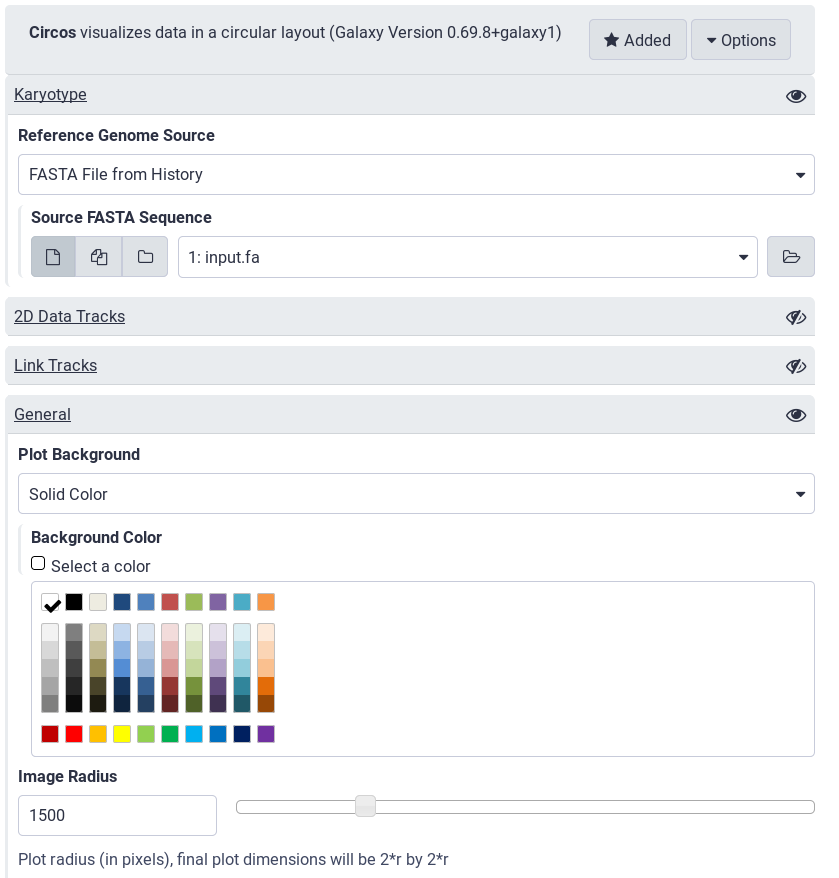
\includegraphics[width=0.8\linewidth]{chapters/images/circos/circos-galaxy-ui.png}
\caption{The Galaxy tool interface to Circos. Each collapsed section hides a wealth of configuration options available to users. The web based interface is significantly more accessible than the command line version.}\label{figure:userinterface}
\end{figure}

We demonstrate the utility of the Galactic Circos tool by recreating one of the more advanced examples from the Circos online tutorials, the microbial genome lesson \cite{circos-microbial-example} (Figure \ref{figure:microbe}). This displays multiple tracks of different types (text, histogram, tiles), has a customized ideogram, and uses rules for colouring data points dependent on their value.

\begin{figure}[h!]
\centering
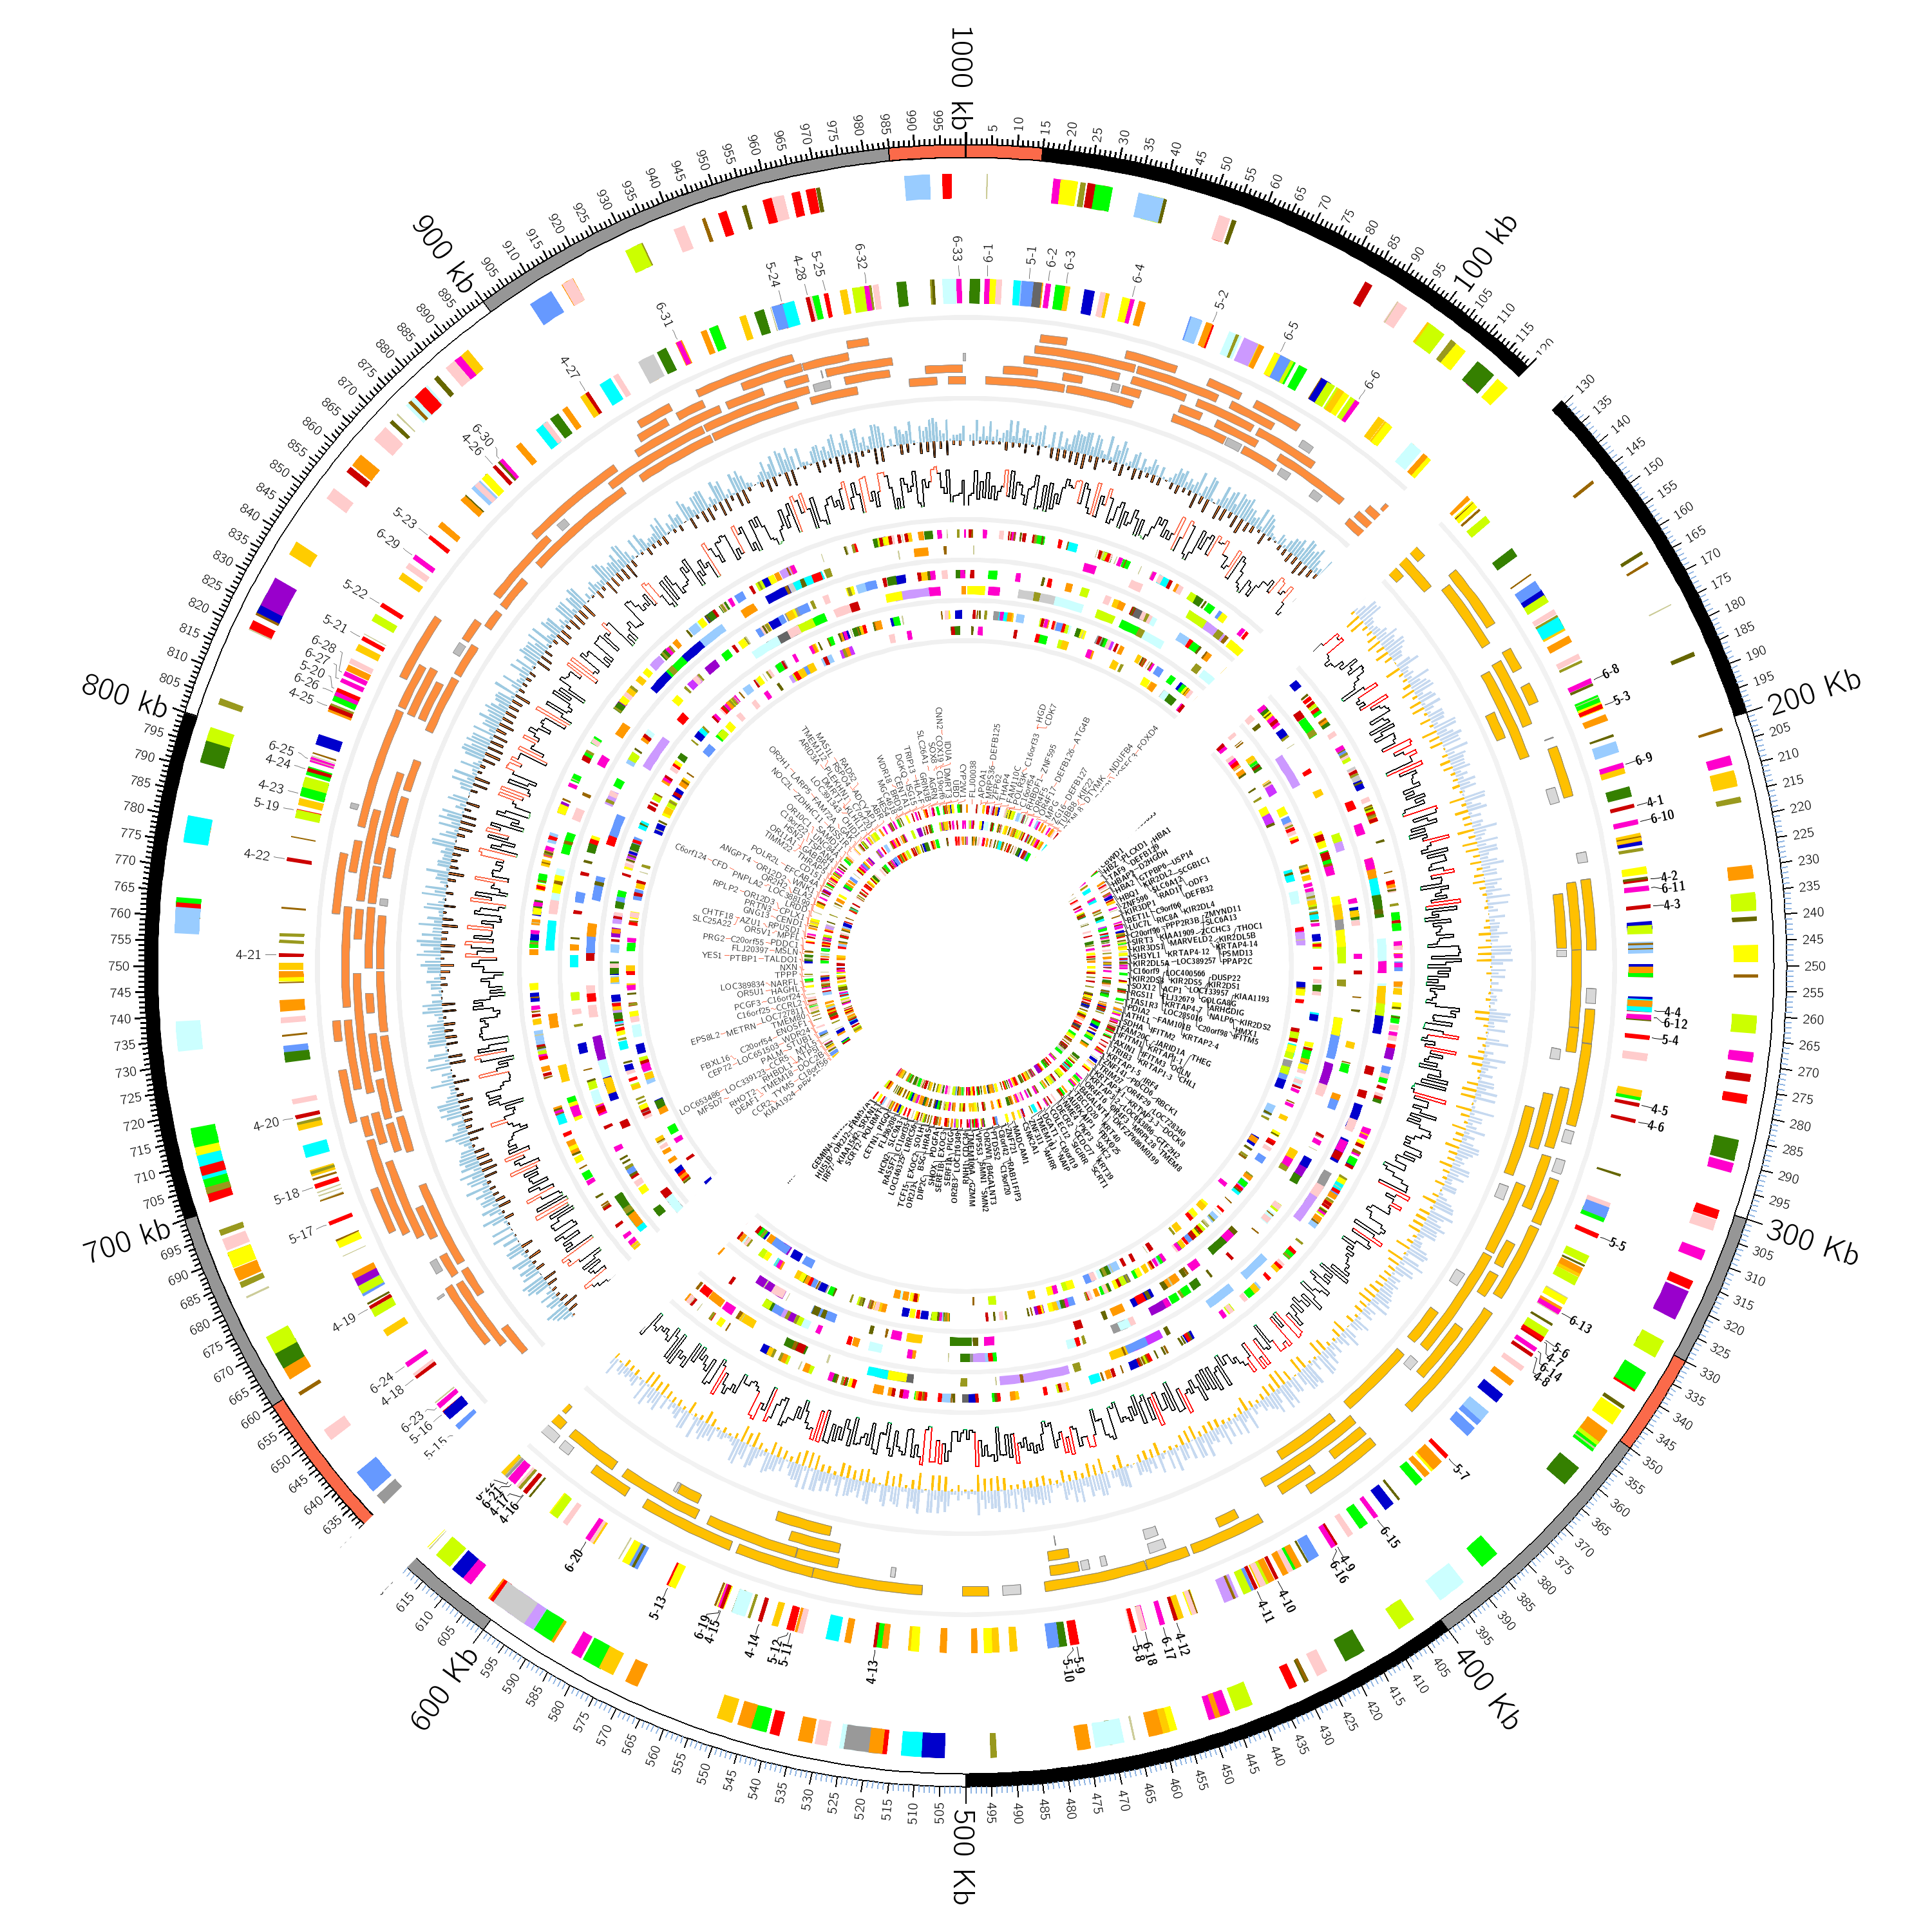
\includegraphics[width=0.8\linewidth]{chapters/images/circos/plot-microbe-both.png}
	\caption{Here we reproduce one of the more complex tutorials from the Circos documentation. The top-left half of the image is produced by the configuration provided by the Circos tutorial, while the bottom-right half is produced completely in Galaxy. While some options used in the original tutorial cannot be directly used (e.g. unrestricted perl code), they can be recreated equivalently in the tool interface. Some options in the tool interface are likewise restricted, Galactic Circos offers a color picker with a limited palette, which explains the differences in colour. However, our tool offers the ability to download the full Circos configuration folder, allowing advanced users to tweak the colour (or other) parameters manually and rebuild the image locally.}\label{figure:microbe}
\end{figure}

In a second example (Figure \ref{figure:encode}), we replicate within Galaxy the cover image of the Nature issue \cite{nature-encode} dedicated to the ENCODE project \cite{encode2004encode}. This cover featured a Circos plot and is also available as part of the official Circos tutorials \cite{circos-nature-example}.

\begin{figure}[h!]
\centering
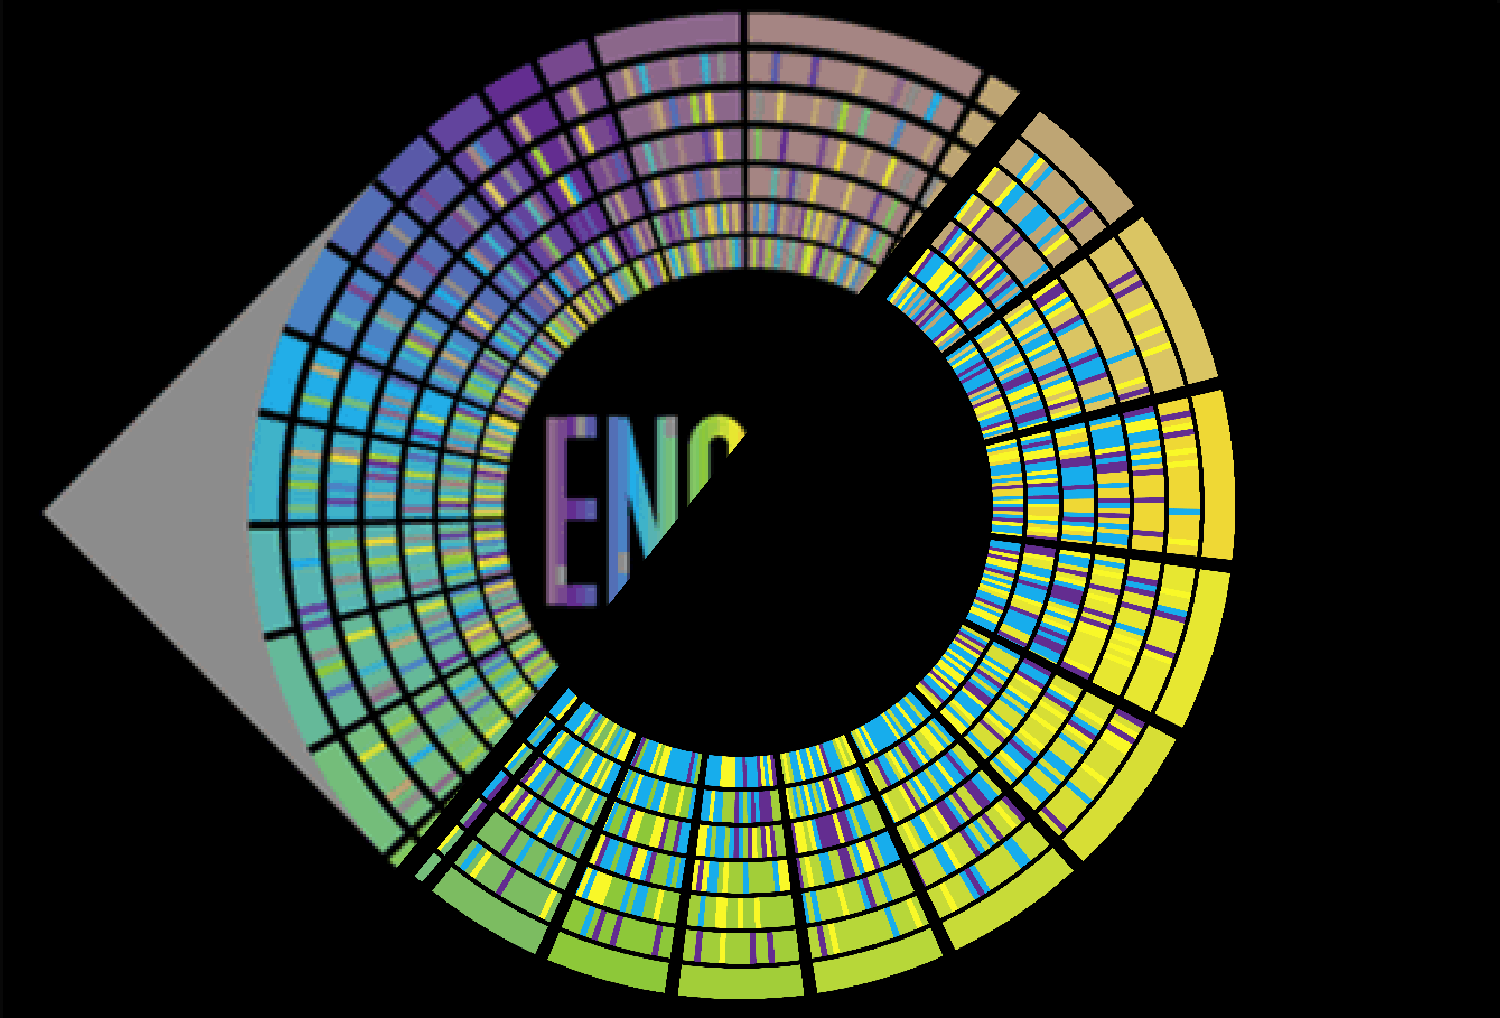
\includegraphics[width=0.7\linewidth]{chapters/images/circos/plot-encode-both.png}
\caption{Nature's cover for the ENCODE project in September 2012, reproduced by Galactic Circos. The top-left half of the image is again directly from the cover, whilst the bottom-right half shows the reproduction of the image using the Galactic Circos tool. The full image could be reproduced in Galaxy accurately, if one wished.}
\label{figure:encode}
\end{figure}

These two examples showcase a variety of different track types (histograms, scatterplot, highlights, tiles, text) and configurations (ticks, rules, ideogram customizations) to illustrate the feature-completeness of Galactic Circos. % "What features" -A

\subsubsection{Supporting Tools}
Circos requires input datasets to adhere to a specific and custom file format. In order to facilitate the conversion of data to this custom Circos format, we have developed several supporting Galaxy tools for conversion. These tools allow users to convert their datasets from a variety of common genomics formats such as (big)Wig files, interval files, and MAF alignments. Furthermore, the existing Galaxy ecosystem provides a wide array of tabular data manipulation tools that can be leveraged to transform any tabular or text files into the format accepted by Circos.

To demonstrate the utility of these supporting tools, we show a real-world example of a plot using common genomics datasets. This example is a recreation of a plot in a published paper demonstrating chromothripsis in the VCaP prostate cancer cell line \cite{alves2013gene}. The input datasets originate from a variety of sources, including a structural variants files (converted to Circos links track), copy number and B-allele frequency track obtained from Affymetrix SNP array data, and a SNP density track generated from a VCF file. Using a combination of the supporting tools included in the Galactic Circos package and the generic file manipulation tools present in Galaxy, we were able to convert these various datasets to circos format without leaving Galaxy, and reproduced the Circos plot from the publication (Figure \ref{figure:vcap}).

\begin{figure}[h!]
\centering
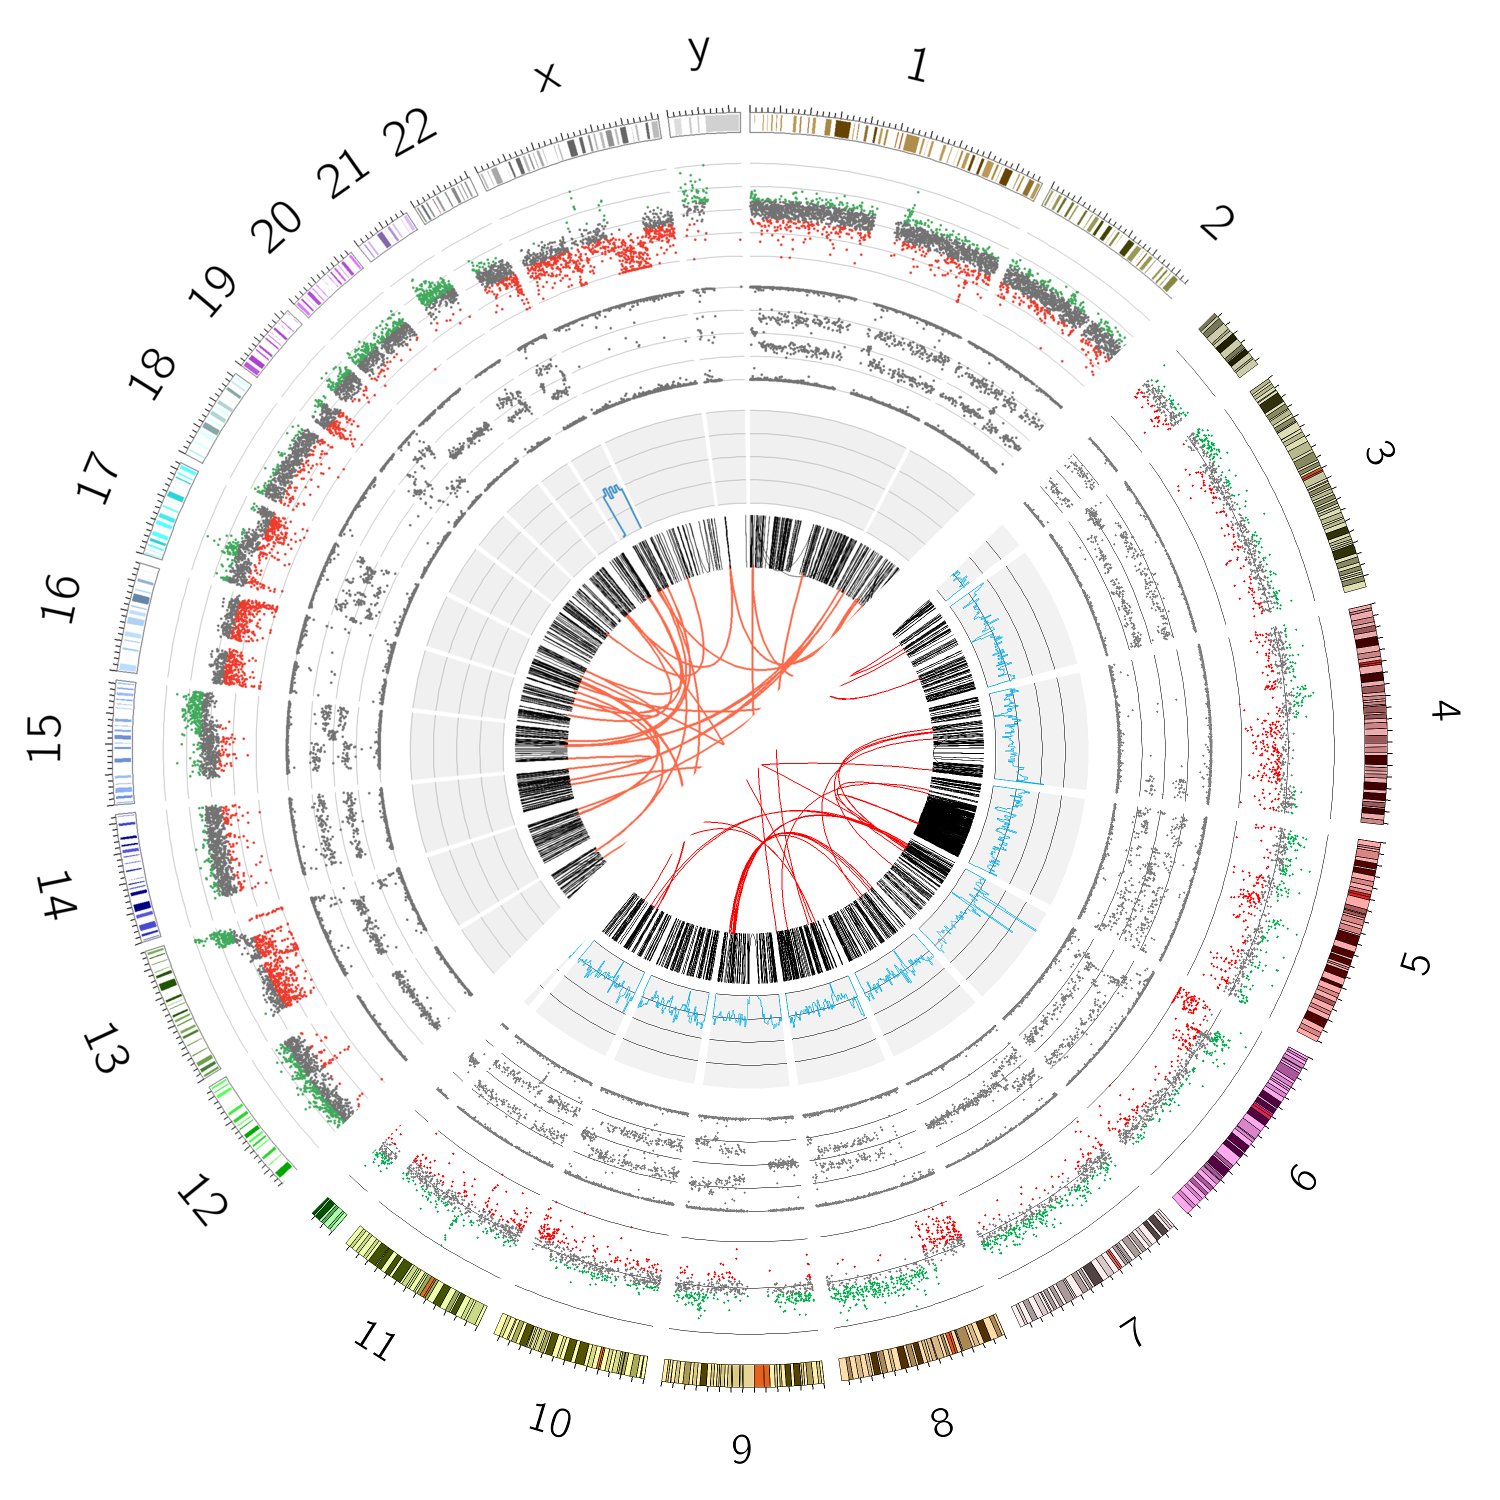
\includegraphics[width=0.6\linewidth]{chapters/images/circos/plot-complete-genomics-both.png}
	\caption{This figure compares output of a custom written Circos plot with hardcoded configuration (top left half), to ťhe output created using the Galactic Circos tool (bottom right half). While the input data originated from a range of standard and nonstandard genomic file formats, conversion to circos-formatted files was possible using the plethora of file manipulation tools already integrated into Galaxy and the set of supporting conversion tools included in the Galactic Circos package.}
\label{figure:vcap}
\end{figure}

Once data has been reformatted for Circos, it can either be used immediately or be further processed. Circos includes a tool suite for post-processing and downsampling of data which can improve plot clarity and processing speed. We additionally wrapped a number of these post-processing tools into Galaxy, notably the link bundling and binning scripts seen in Figure \ref{figure:binning-bundling}.

\begin{figure}[h!]
\centering
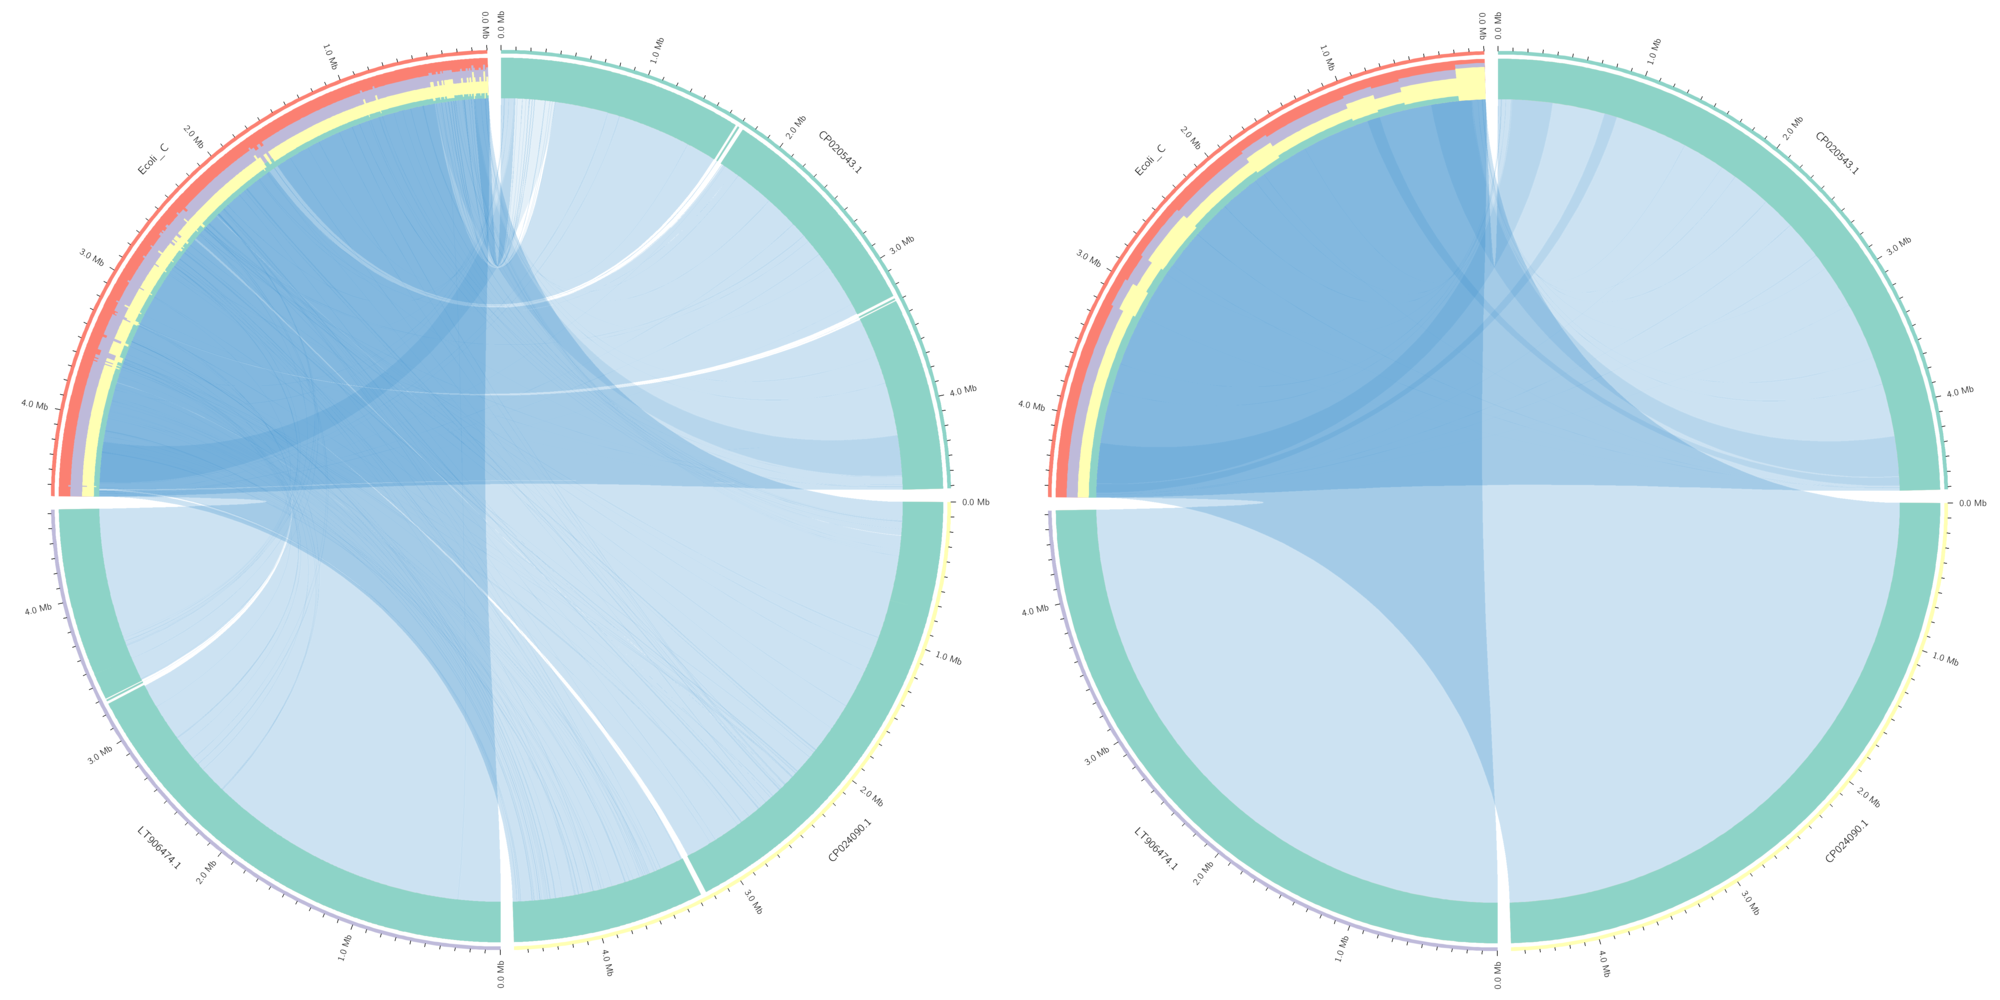
\includegraphics[width=\linewidth]{chapters/images/circos/binning-bundling.png}
\caption{These two plots show the link binning and bundling scripts used with different thresholds. The inner link track was generated directly from a MAF file output by LastZ \cite{rahmani2011lastz}. This file was processed by Circos' bundling tool in Galaxy in order to decrease the number of links, a process usually done to decrease visual noise and increase efficiency. The outer track demonstrates the link binning script which generates a histogram, in this case from the number of links to that position in the genomic region.}
\label{figure:binning-bundling}
\end{figure}

Finally, while Circos is widely used for the visualization of genomic data, and many of the parameter names have a distinctly biological feel to them, the tool does not impose any restrictions on the type of input data, and is capable of displaying non-biological data just as easily \cite{circosnongenomic}. To show that our tool retains this degree of flexibily, we recreated the presidential debate plot included in the Circos tutorials, which in turn was based on a plot which appeared in the New York Times aticle \cite{namingnames}. A plot comparison can be seen in Figure \ref{figure:debate}.

\begin{figure}[h!]
\centering
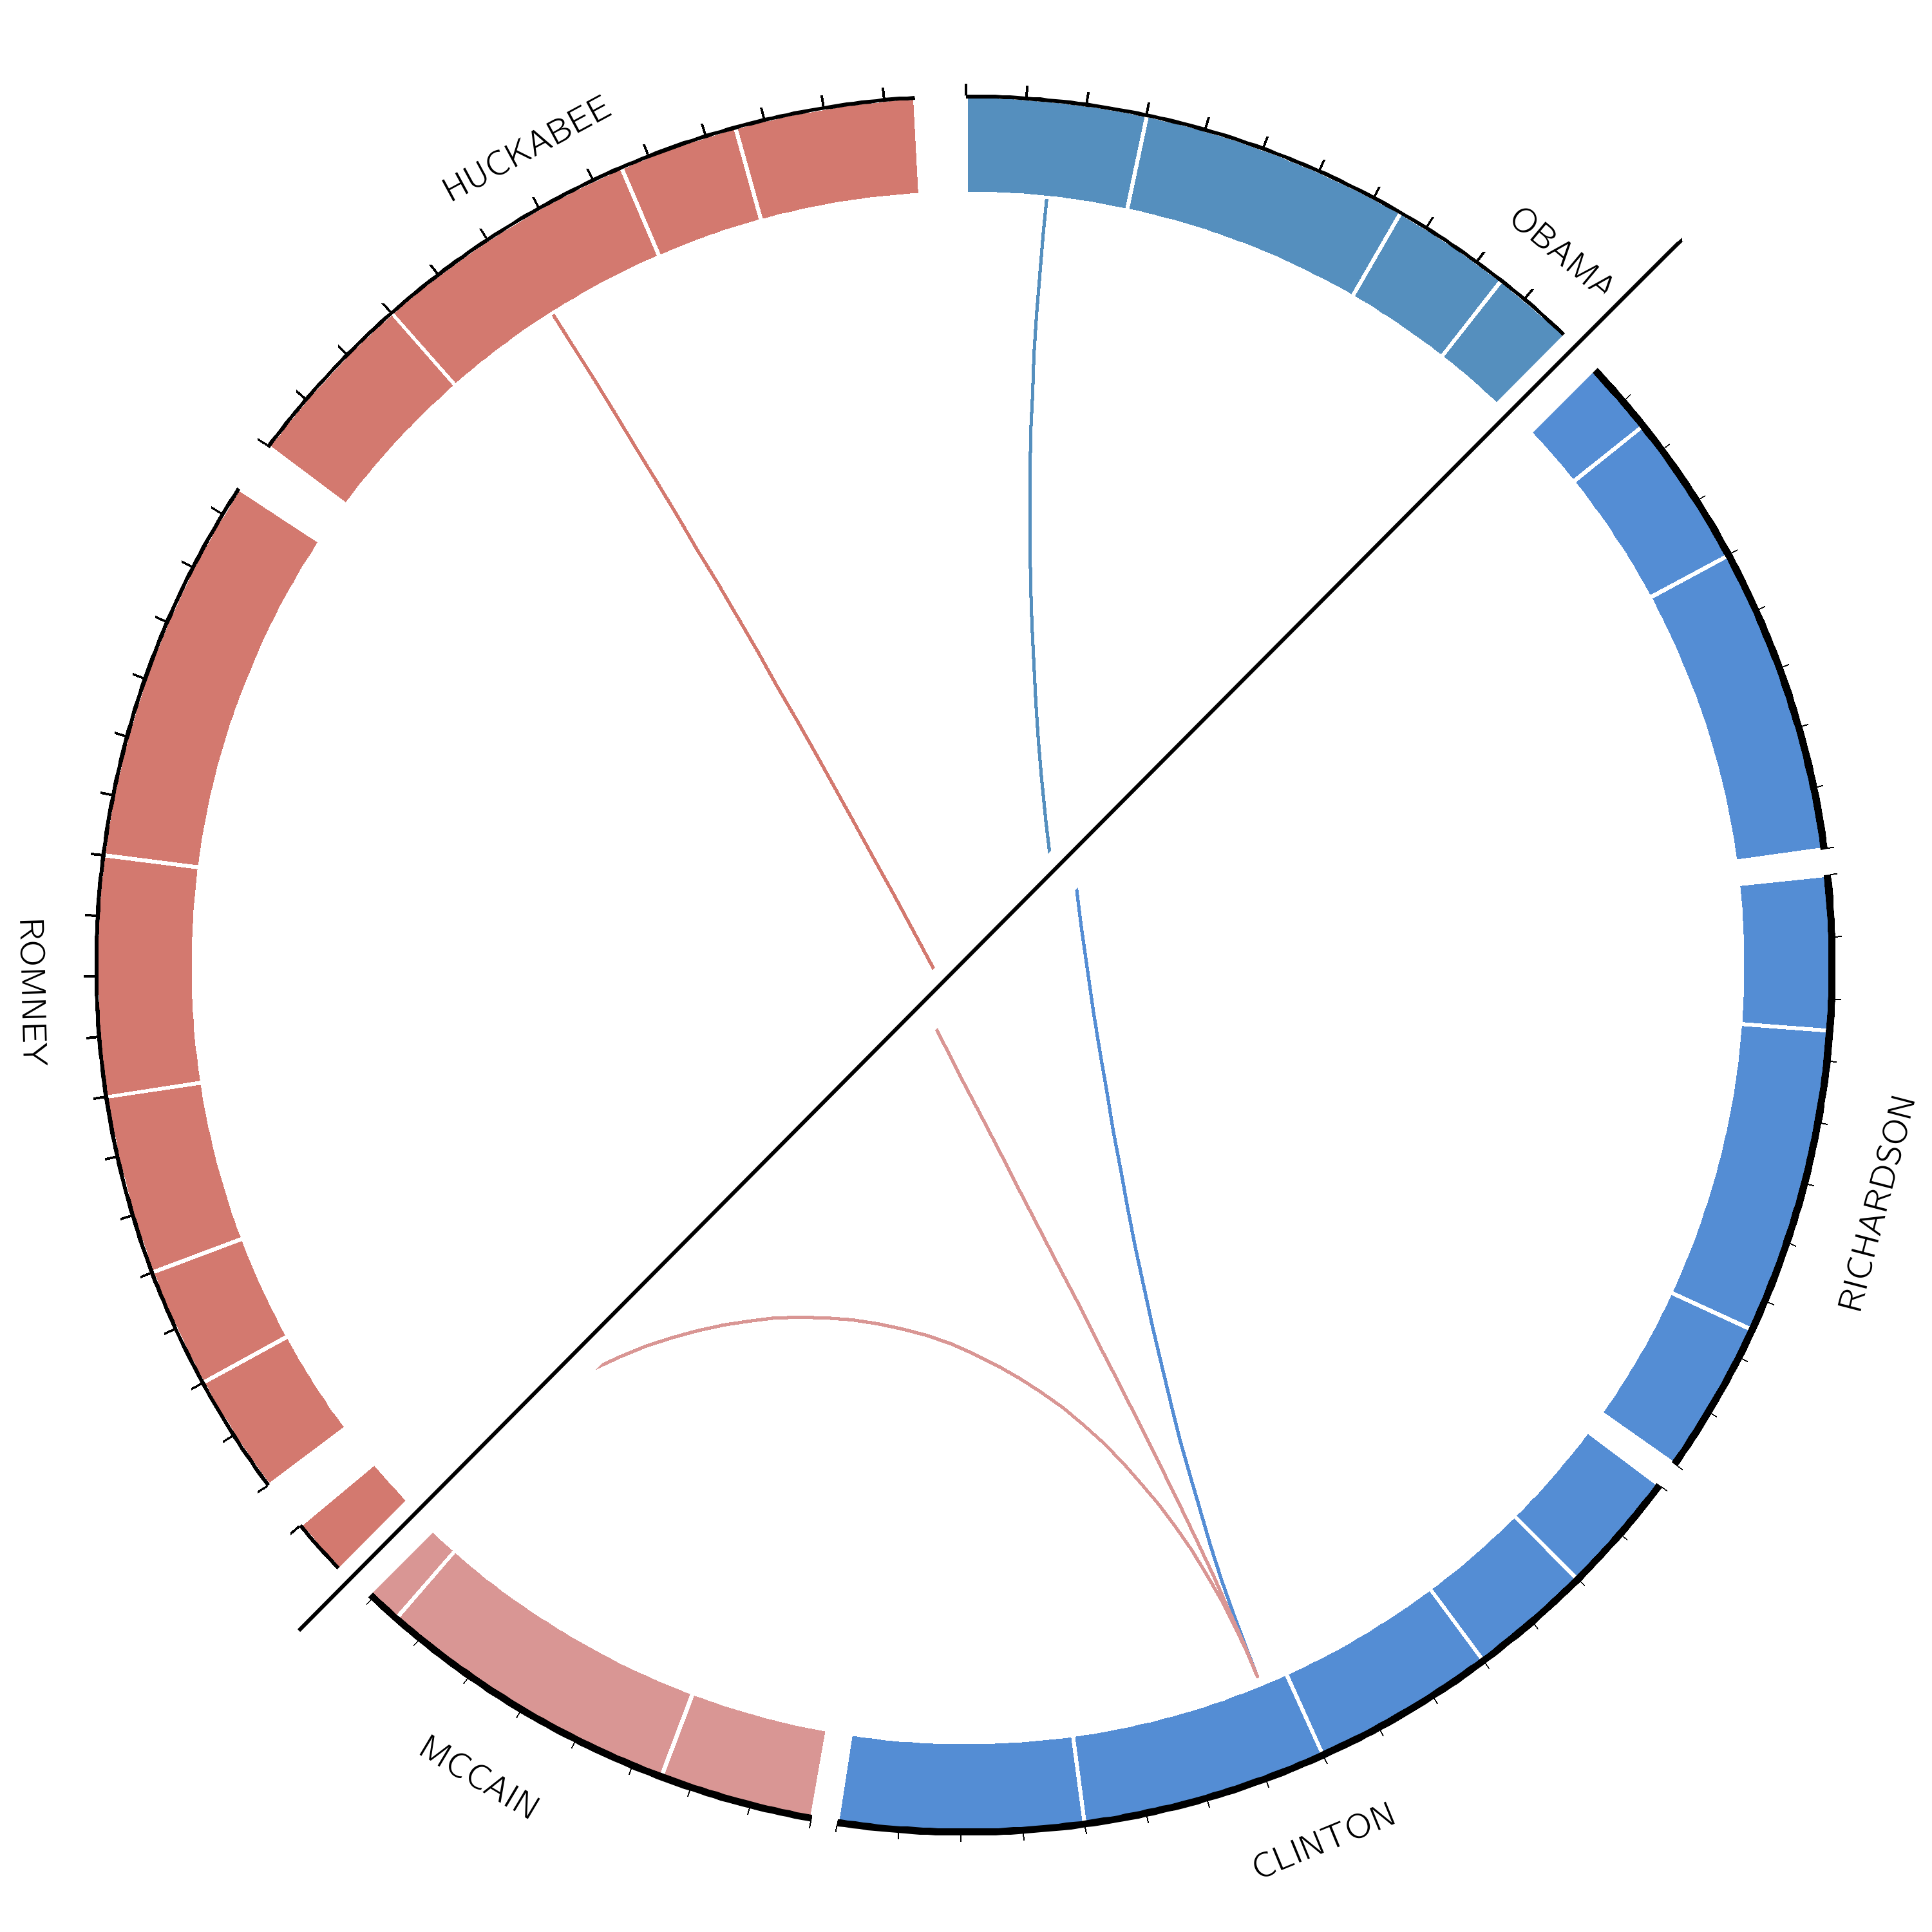
\includegraphics[width=0.6\linewidth]{chapters/images/circos/plot-politics-both.png}
\caption{This figure compares the Circos plot from the official tutorial (top left half), to ťhe output created using the Galactic Circos tool (bottom right half). Each link represents a candidate speaking the last name of another candidate. The length of each circle segment is proportional to the total number of words spoken by the candidate during the debates.}
\label{figure:debate}
\end{figure}

\section*{Methods}

\subsection*{Implementation}
The execution of the tool leverages Galaxy's ability to write templated files directly to disk with configuration from the tool form, and then running Circos directly on these templated configuration files.

Installation of the Circos tool and its dependencies is handled by the Galaxy platform and utilizes the Conda framework for dependency management. All dependencies including circos itself are available from the Bioconda Conda channel \cite{gruning2018bioconda} and available as a virtualised container (rkt, Docker, Singularity).

\subsection*{File Format Converters}
In order to facilitate the interoperability with upstream tools and workflows, we provide a set of file format converters, in addition to many tools already available in Galaxy, which together provide for convertion of a range of common data format standards (e.g. VCF, MAF/Stockholm, BED/GFF3, BigWig). These tools produce files that are ready to be used as input to the Galaxy Circos tool. Additionally the applicable subset of circos-utils were included into Galaxy for Circos-friendly tools for data reshaping.

\subsection*{Circos Configuration Export}
While Galactic Circos aims to offer the full range of Circos functionality, some manual tweaking of the Circos plot configuration files may still be desired. To this end, our tool also outputs the full set of configuration files needed to recreated the plot on the command line, and thus allow easy access to any features not exposed in the Galaxy wrapper.

\subsection*{Training Materials}
Our tool greatly simplifies the creation of Circos plots, but the great number of options offered by the Circos tool require good documentation and explanation in order to optimize their utility for end-users. Circos offers a collection of tutorials that are designed to familiarize users with the various features of Circos \cite{circostutorials}. In a similar fashion, we have created a set of Galaxy tutorials aimed to educate users in the use of Circos within Galaxy. These tutorials are available from the Galaxy training materials website \cite{Batut2018}.

\subsection*{Reproducible and Reusable Plots}
To enable readers to examine the complete parameters settings used and recreate the example plots given here, Galaxy histories for all the figures shown in this work have been made publicly available from the European Galaxy server \cite{TODO} (see Availability section).

\subsection*{Future Work}
While we have aimed to make our tool as feature-complete as possible, some of Circos' functionality is not currently exposed in the Galaxy tool. We intend to extend our tool to include these features, including but not limited to support for scaling subsections of the plots, and generation of HTML image maps.

\section*{Availability of source code and requirements}
\begin{itemize}
\item Project name: ~Galactic Circos
\item Github repository:~\url{https://github.com/galaxyproject/tools-iuc/tree/master/tools/circos}
\item Tool Shed repository: ~\url{ https://toolshed.g2.bx.psu.edu/view/iuc/circos}
\item Training Manual: ~\url{https://training.galaxyproject.org/<TODO>}
\item Operating system(s): ~Unix (~Platform independent with Docker)
\item Other requirements: ~Galaxy version 18.01 or higher
\item License: ~GNU GPL
\end{itemize}

The Circos example plots presented in this work are available as Galaxy histories:

\begin{itemize}
\item Galaxy history for Figure 2: https://usegalaxy.eu:/u/helena-rasche/h/circos-microbe-tutorial
\item Galaxy history for Figure 3: https://usegalaxy.eu/u/helena-rasche/h/circos-encode-nature-cover
\item Galaxy history for Figure 4: https://usegalaxy.eu/u/helena-rasche/h/circos-cancer-genomics--chromothripsis
\end{itemize}

\section*{Availability of supporting data and materials}

The data presented here to illustrate our application was obtained from previous publications, and has been collected and made available from Zenodo \cite{TODO}.

\section*{Declarations}

\subsection*{List of abbreviations}

\begin{itemize}
\item NGS: Next Generation Sequencing
\item VCF: Variant Call Format
\item MAF: Multiple Alignment Format
\end{itemize}

\subsection*{Competing Interests}
The authors declare that they have no competing interests.

\subsection*{Funding}
This project was made possible with the support of the Albert Ludwig University of Freiburg.

This project has received funding from the European Union’s Horizon 2020 research and innovation programme under grant agreement 825775.

\subsection*{Author's Contributions}

HR and SH contributed to the tool development and writing of the manuscript.

\section*{Acknowledgements}

The authors would like to thank the Galaxy community for their help in reviewing, testing, and validating the tools presented here.

\bibliographystyle{ieeetr}
\bibliography{references}

  \cleartorightpage
%reset references counter
\setcounter{NAT@ctr}{-1}

\chapter*{}\label{chapter:ireport}
\phantomsection
\addcontentsline{toc}{section}{iReport}
%%%%%%%%%%%%%%%%%
%    iReport
%%%%%%%%%%%%%%%%%

\begin{figure}[t!]
\centering

\includegraphics[height=10em]{frontmatter/images/chapter-header-ireport.png}
\end{figure}
\vspace{-4cm}

\articletitle{iReport: A generalised Galaxy solution for integrated experimental reporting}
Saskia Hiltemann\textsuperscript{\ref{ireport-affil:emc-bioinf},\ref{ireport-affil:emc-urology}},
Youri Hoogstrate\textsuperscript{\ref{ireport-affil:emc-bioinf},\ref{ireport-affil:emc-urology}},
Peter van der Spek\textsuperscript{\ref{ireport-affil:emc-bioinf}},
Guido Jenster\textsuperscript{\ref{ireport-affil:emc-urology}},
Andrew Stubbs\textsuperscript{\ref{ireport-affil:emc-bioinf}}

\textbf{Published in:} \emph{GigaScience}, Volume 3, Issue 1, December 2014, 2047-217X-3-19 \\
DOI: \url{https://doi.org/10.1186/2047-217X-3-19}

\small
\begin{enumerate}
\itemsep-0.5em
\item Department of Bioinformatics, Erasmus Medical Center, Rotterdam, The Netherlands. \label{ireport-affil:emc-bioinf}
\item Department of Urology, Erasmus Medical Center, Rotterdam, The Netherlands. \label{ireport-affil:emc-urology}
\end{enumerate}
\normalsize



\section*{Abstract}

\textbf{Background:} Galaxy offers a number of visualisation options with components, such as Trackster, Circster and Galaxy Charts, but currently lacks the ability to easily combine outputs from different tools into a single view or report. A number of tools produce HTML reports as output in order to combine the various output files from a single tool; however, this requires programming and knowledge of HTML, and the reports must be custom-made for each new tool.\\
\textbf{Findings:} We have developed a generic and flexible reporting tool for Galaxy, iReport, that allows users to create interactive HTML reports directly from the Galaxy UI, with the ability to combine an arbitrary number of outputs from any number of different tools. Content can be organised into different tabs, and interactivity can be added to components. To demonstrate the capability of iReport we provide two publicly available examples, the first is an iReport explaining about iReports, created for, and using content from the recent Galaxy Community Conference 2014. The second is a genetic report based on a trio analysis to determine candidate pathogenic variants which uses our previously developed Galaxy toolset for whole-genome NGS analysis, CGtag. These reports may be adapted for outputs from any sequencing platform and any results, such as omics data, non-high throughput results and clinical variables.\\
\textbf{Conclusions:} iReport provides a secure, collaborative, and flexible web-based reporting system that is compatible with Galaxy (and non-Galaxy) generated content. We demonstrate its value with a real-life example of reporting genetic trio-analysis.


\section*{Findings}

Structured reporting and documentation of experimental outcome is required for the successful transfer of knowledge from the research scientist to their peers and to the broader academic community.

Galaxy is a platform that aims to provide complex bioinformatics services and tools in an easy-to-use web-based graphical user interface~\cite{goecks2010galaxy,blankenberg2010galaxy,giardine2005galaxy}. The output from these tools can be displayed using built-in Galaxy visualisation applications~\cite{goecks2013web}, via specialised visuals implemented as a component in the workflow deployed in Galaxy~\cite{cgtag} or by downloading the results and visualising the output with applications external to Galaxy (e.g., Excel, TIBCO spotfire, R, spreadsheet programs, \emph{etc}).

Galaxy has the capacity to track the provenance of the source data, the workflow, as well as the workflow components used to analyse the data. Currently users can share their workflow and results within Galaxy, but do not have access to a simple method to summarise results from multiple tools and/or workflows in an integrated report. To address this issue we have developed iReport, an integrated reporting application that provides users with a flexible means to produce dynamic HTML reports which can be shared with other Galaxy users or downloaded to disk.

Systems used by end-users to deliver graphical output range from open-source applications, such as \emph{Ad Hoc} reports~\cite{url-adhoc}, Google charts (and docs)~\cite{url-googlecharts} and OpenOffice~\cite{url-openoffice}, to commercial applications such as Microsoft Office.
Indeed scientific reporting applications both open-source (Bioconductor~\cite{url-bioconductor}, Circos~\cite{circos}\cite{url-circos}) and commercial software (e.g., Omniviz~\cite{url-omniviz}, Partek~\cite{url-partek}) include a multitude of visualisation capabilities with a focus on data reporting and presentation of data in the context of the experimental design and with associated meta-data.
There are some applications, like TIBCO spotfire~\cite{url-spotfire}, which are capable of integrating results from multiple sources including associated text and meta-data and other applications which serve as an electronic lab note book (e.g., IDBS~\cite{url-idbs}).
Additionally there have been many products developed to address the selection and reporting of variants for pathogenic variant selection including the workflow to identify those variants (e.g., Gensight~\cite{url-gensight}, Cartagenia~\cite{url-cartagenia}, Clincial Genomicist~\cite{clinicalgenomist}).
For data generated in R, dynamic reporting packages such as KnitR~\cite{url-knitr}, Sweave~\cite{sweave} and R-Markdown~\cite{url-rmarkdown}, allow for the integration of data-generating code within the report specification itself. Similar systems exist for other programming languages, for example Tangle~\cite{url-tangle} (JavaScript), Active Markdown~\cite{url-activemarkdown}(CoffeeScript) or IPython Notebooks~\cite{url-ipythonnotebook} (Python).
These are very versatile tools, but require programming knowledge to use effectively. iReport offers an open-source application for both Galaxy and non-Galaxy produced results allowing for the generation of customized integrated reports for any type of project or workflow.
The advantage to Galaxy users is that the output from any application can be included into any report, and that a report template can be reused for other projects.
Also, the report may be securely shared with one or many users of that Galaxy instance or made publicly available.\ iReports can be completely configured from the tool web interface, and requires no programming or knowledge of the underlying system.

We demonstrate iReport’s utility through an example where a genetic report is generated from outputs of an existing Galaxy next-generation sequencing (NGS) toolkit, CGtag~\cite{cgtag}. iReport can also be used as an electronic lab notebook by creating an iReport which links out to various other iReports containing different analysis reports from various samples. It can be also be coupled to output from other Galaxy instances, for example output generated by specialized Galaxy instances such as Confero~\cite{confero}, ORIONE~\cite{orione}, and Galaxy-P~\cite{url-galaxyp}.

\section*{Functionality}
iReport dynamically generates HTML, and employs JavaScript and jQuery to create interactive components, such as searchable, sortable, paginated tables and zoomable images.\ iReport is ideally suited to use as the final step in a workflow; the pipeline developer configures the report once and end-users are then presented with a templated report each time users run the workflow, while only needing to provide the input files for the pipeline~\cite{CGtagpipeline}. iReport can also be used directly by end-users as a means of easily sharing their results with other Galaxy users, or the public via Galaxy's native sharing capabilities.

The generic reporting functionality and usage of iReport is outlined below using an example iReport created for the recent Galaxy Community Conference, which is also available for viewing online~\cite{url-ireport-tutorial}. It is followed by an example of a genetic report that can be used for trio analysis, which can easily be modified for any trio reporting or extended to quartets or larger families, also available from our demo galaxy~\cite{url-genetic-ireport}.

\section*{iReport Structure}

iReport produced a report webpage consisting of one or more subpages with one or multiple elements included on each subpage. The primary output of iReport is:


\begin{enumerate}
 \item A cover page
  \begin{enumerate}
    \item Title of the report
    \item Cover image
  \end{enumerate}
 \item Main report page consisting of a set of tabs. Each tab consisting of one or more \emph{content items}. Each content item can be one of the following types:
  \begin{enumerate}
    \item Text
    \item Images
    \item Tables
    \item PDF Files
    \item Links
  \end{enumerate}
\end{enumerate}

An iReport tutorial has been developed to demonstrate and explain the functionality of iReport, and is available as a shared history from the CTMM-TraIT public Galaxy instance~\cite{url-ireport-tutorial}. The following sections describe each of the components of iReport in more detail.

\subsection*{Cover Page}
The cover page consists of a user-specified title and a cover image. The cover image parameter is optional and when the field is left blank a default image is used (\hyperref[fig:defaultcover]{Figure~\ref*{fig:defaultcover}}).
By clicking on the image, or the link above it, the user can access the main report page. There is also a link to download the entire iReport webpage, including all dependency files, for storing or viewing on different systems.

\begin{figure}[h!]
    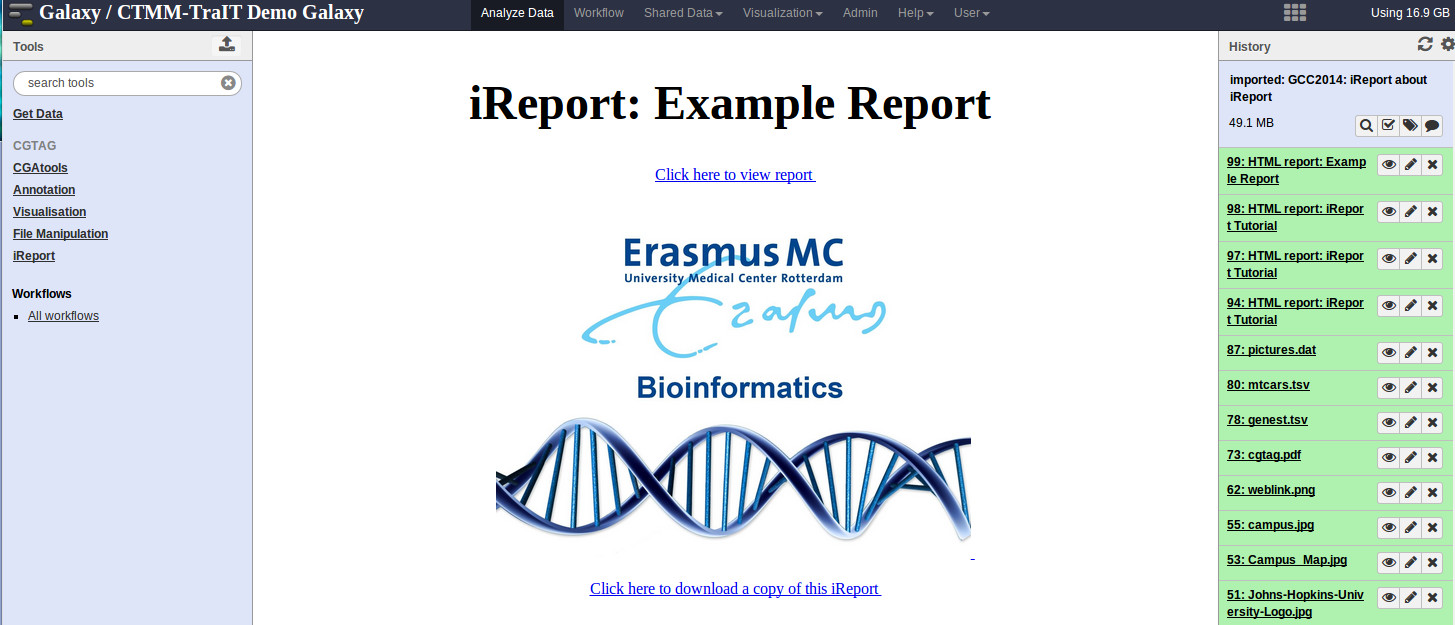
\includegraphics[width=0.95\textwidth]{chapters/images/iReport/Hiltemann_defaultcover.jpg}
    \caption{Example cover page.Example of a cover page with title \emph{Example Report} and the default cover image. A link to download the entire iReport web page is also provided.}
    \label{fig:defaultcover}
\end{figure}


\subsection*{Main Report Page}
An arbitrary number of tabs may be added via a repeat parameter. Each tab can be labelled with a name specified by the user. An arbitrary number of \emph{content items} may then be added to each tab in a repeat parameter. A type must be specified for each content item (e.g., text, image, table \emph{etc.}), as well as several other parameters depending on the type chosen (\hyperref[fig:wrapper]{Figure~\ref*{fig:wrapper}}). Layout is mostly left up to the browser, but users can explicitly add a line-break after each item to force items to appear underneath each other.

% Galaxy wrapper
\begin{figure}[h!]
    \centering
    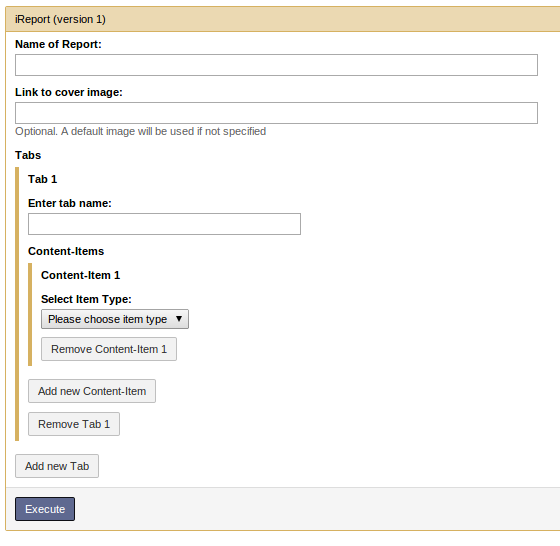
\includegraphics[scale=0.4]{chapters/images/iReport/Hiltemann_wrapper.jpg}
    \caption{iReport tool wrapper. iReport's tool interface. Minimally a report title and at least 1 tab with 1 content item need to be specified.}
    \label{fig:wrapper}
\end{figure}

\paragraph*{Content item: Text Field}
Text can be entered in a text field in the tool interface, for example to create an introduction paragraph and to give a description of the items on the page. Text is printed verbatim, although a small number of HTML tags are allowed in order to give the user some control over formatting (e.g., \verb+b, i, em, strong, h1-h6+ tags). Text files can also be specified, and the contents of the file will be printed to the screen verbatim.

\paragraph*{Content item: Images}
Many tools produce images as output, which can also be displayed by iReport. Users specify the image file from their Galaxy history, and the desired image size. For images that have been scaled down, an optional jQuery zoom-on-mouseover effect may be added (\hyperref[fig:imagezoom]{Figure~\ref*{fig:imagezoom}})\cite{url-jqueryzoom}. Currently supported image formats are JPG, PNG and SVG.

%% zoomeffect
\begin{figure}[h!]
    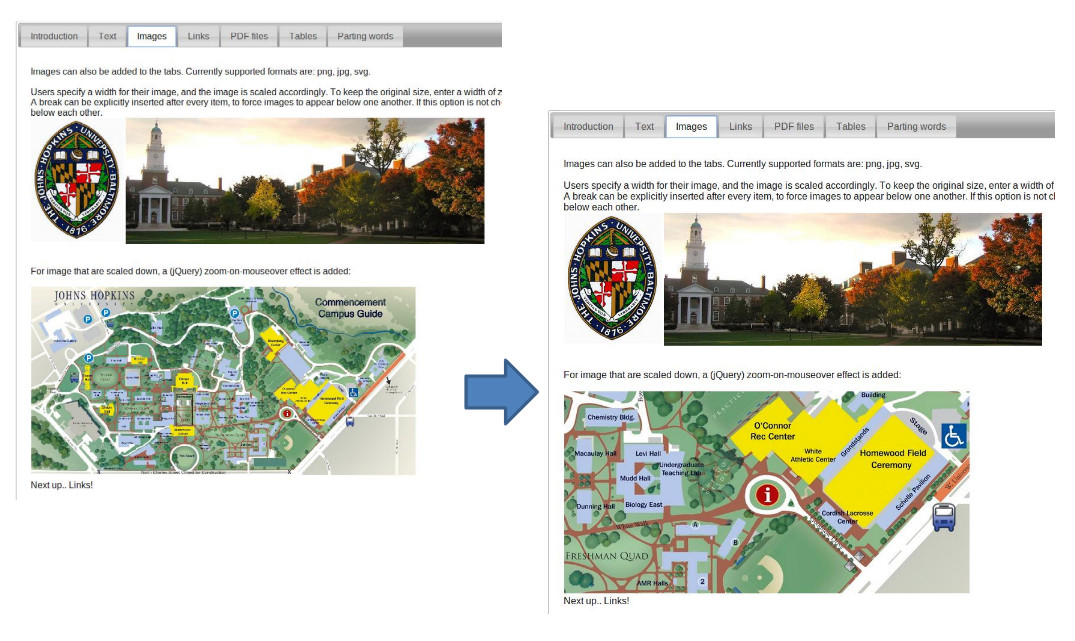
\includegraphics[width=\textwidth]{chapters/images/iReport/Hiltemann_zoomeffect.jpg}
    \caption{Zoom effect.Images that have been scaled down can optionally be enhanced with a jQuery zoom-on-mouseover effect. In this example, the bottom image has this effect added, and when the user moves their mouse over the image, a zoomed version of that area of the image is shown.}
    \label{fig:imagezoom}
\end{figure}

\paragraph*{Content item: Tables}
iReport can also display tables. The input must be a tab-delimited file from the users' Galaxy history, and the first nonempty line not starting with a hash symbol (\verb+#+) is assumed to contain the column headers. The jQuery library \emph{DataTables}~\cite{url-datatables} is used to create tables which can be searchable, sortable and paginated, if requested by the user. There is an option to create hyperlinks within the columns of a table by providing a column number, a URL prefix and a URL suffix. This is illustrated in \hyperref[fig:collinks]{Figure~\ref*{fig:collinks}}, where the first column contains gene names and by including the GeneCards~\cite{genecardspaper,url-genecards} URL prefix \verb+http://www.genecards.org/+ \verb+cgi-bin/carddisp.pl?gene=+. This generates a hyperlink to the corresponding GeneCards entry for every item in the column in the table.

%% weblinks from table columns
\begin{figure}[h!]
    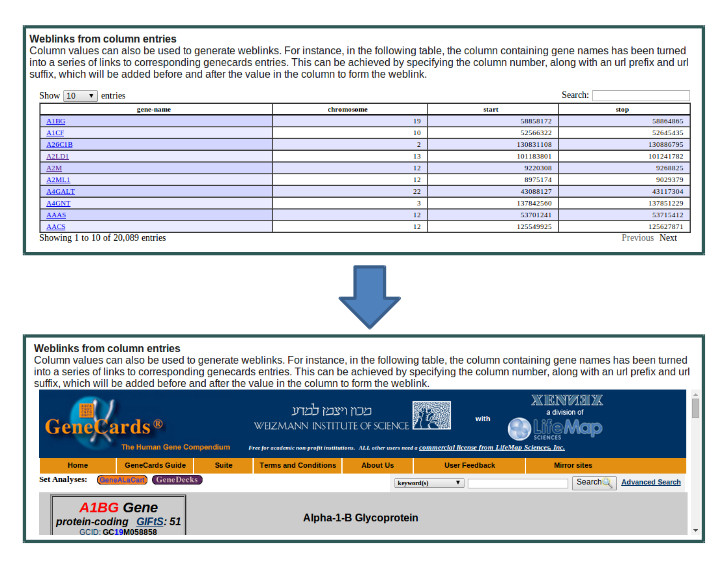
\includegraphics[width=0.95\textwidth]{chapters/images/iReport/Hiltemann_columnlinks.jpg}
    \caption{Weblinks from table columns
   A series of web links can be created within a table by specifying a prefix and suffix to be placed before and after each column entry.}
    \label{fig:collinks}
\end{figure}

\paragraph*{Content item: PDF Files}
This is one of the simplest content items. The user provides a PDF file from the Galaxy history, which will be embedded in the page. If the browser does not have the necessary plug-ins installed, a download link for the file will be generated instead (\hyperref[fig:pdfexample]{Figure~\ref*{fig:pdfexample}}).

%% PDF example
\begin{figure}[h!]
    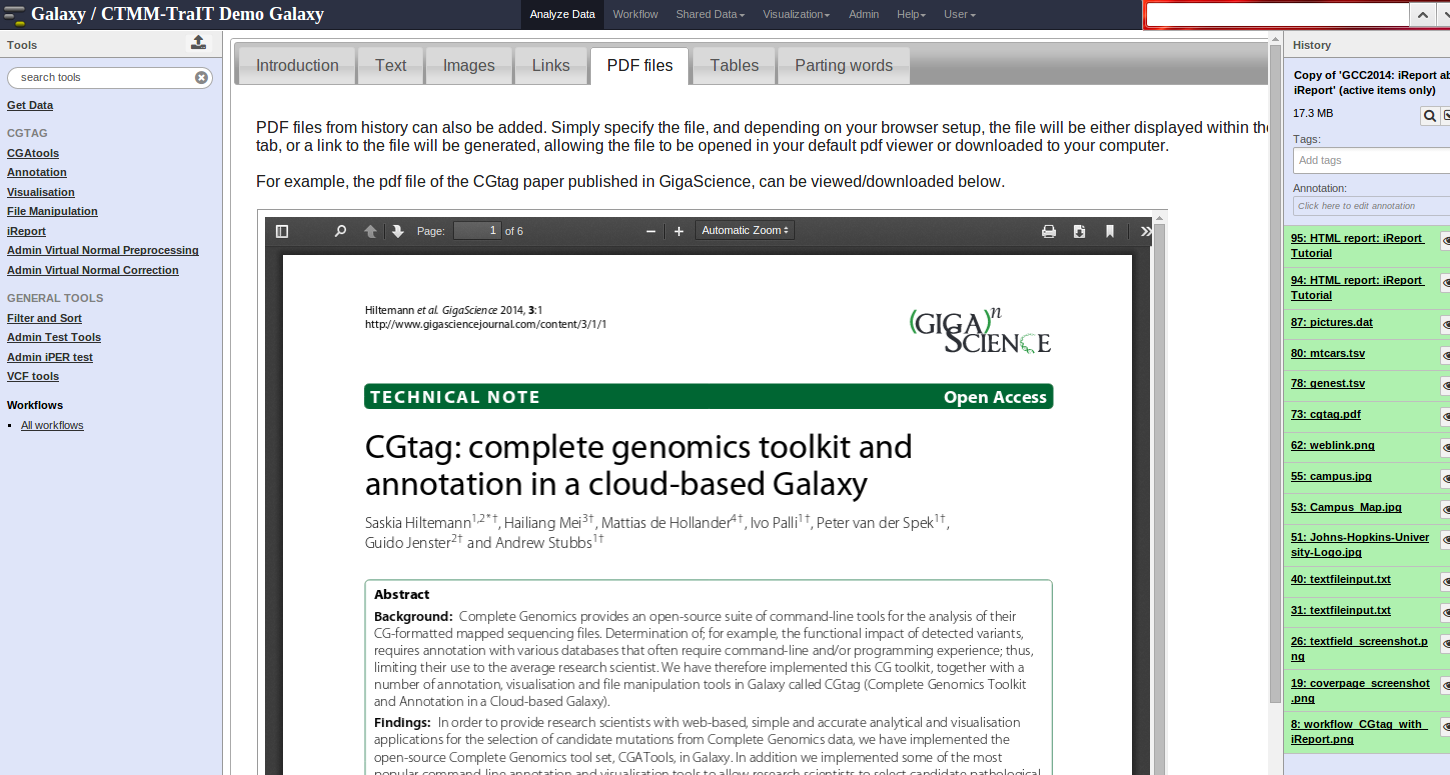
\includegraphics[width=\textwidth]{chapters/images/iReport/Hiltemann_PDF.jpg}
    \caption{Embedded PDF files. iReports can also display PDF files. For browsers without PDF plug-in, a download link to the file will be created instead. }
    \label{fig:pdfexample}
\end{figure}

\paragraph*{Content item: Links}
Users can create links to web locations by specifying a URL and a link text. Links to datasets in the history can also be created here by specifying a dataset and a link text. Several tools create archives of files as output (for example a zip file containing the plots for each chromosome). Links to all files contained in an archive can also be created, and will be named with the file names (excluding file extension). Currently the supported archive formats are zip, bz2, tar, gz and tar.gz. An example can be seen in \hyperref[fig:archivelinks]{Figure~\ref*{fig:archivelinks}}, where an archive with images was used as input and a series of links to each contained file was created. An option to create a link to an iReport is also present. This allows users to create a kind of electronic lab notebook, by creating an overview of all their samples and linking to one or more iReports for each sample.

%% links from archive
\begin{figure}[h!]
    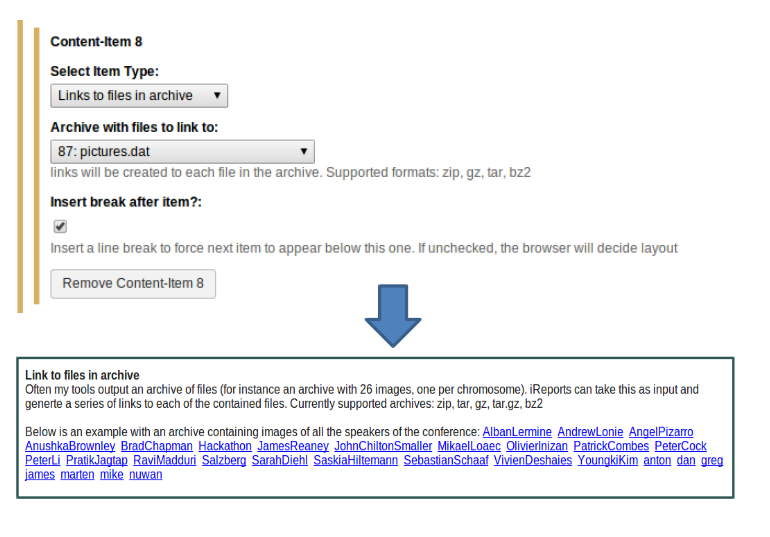
\includegraphics[width=0.8\textwidth]{chapters/images/iReport/Hiltemann_archivelinks.jpg}
    \caption{Links to all files in an archive.Given an archive of files, iReport can create a series of links to all files contained in the archive. Link texts are the filenames (without file extension).}
    \label{fig:archivelinks}
\end{figure}

\section*{Genetic report for a trio of HapMap individuals}

Accurate, reproducible and traceable reporting is an essential requirement to the evaluation of the genetic outcome from any assay~\cite{skyline}, including those variations predicted from NGS analysis. Since iReport is capable of including many formats, we have used the outcome from a trio analysis generated from the Complete Genomics~\cite{drmanac} NGS platform to demonstrate its utility in representing these data in a user-defined format, which contains the provenance of the underlying analysis. In this example we use a trio of individuals sequenced in the International HapMap Project~\cite{hapmap}\cite{hapmap2}, to demonstrate how to select protein affecting candidate variants based on a recessive genetic model.  All data in this example is freely available for download from the Complete Genomics website~\cite{url-CGpublicdata}.

This example iReport has one tab devoted to explaining the protocol used (\hyperref[fig:trioscreenshots]{Figure~\ref*{fig:trioscreenshots}B}), one tab with circos plots and an explanation of the family structure (\hyperref[fig:trioscreenshots]{Figure~\ref*{fig:trioscreenshots}D}), and one tab with tables containing the candidate pathogenic variants determined by the protocol based on a recessive model for selection. This iReport is also available as a published history on the TraIT-CTMM public Galaxy~\cite{url-traitgalaxy}.

%% Genetic Report
% file: Hiltemann_geneticreport[A-D].jpg
\begin{figure}[h!]
   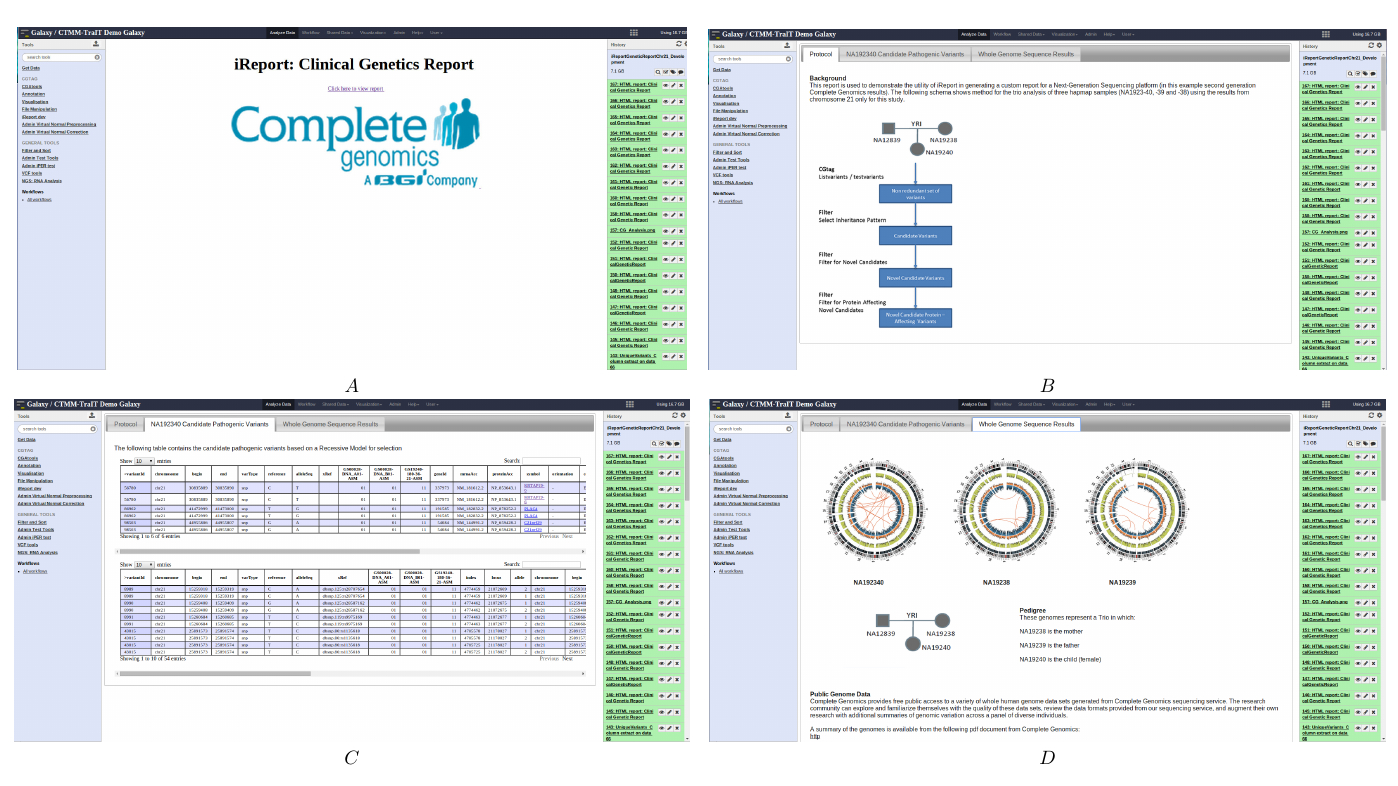
\includegraphics[width=\textwidth]{chapters/images/iReport/Hiltemann_geneticreport.jpg}
%    \begin{center}$
%    \begin{array}{cc}
%    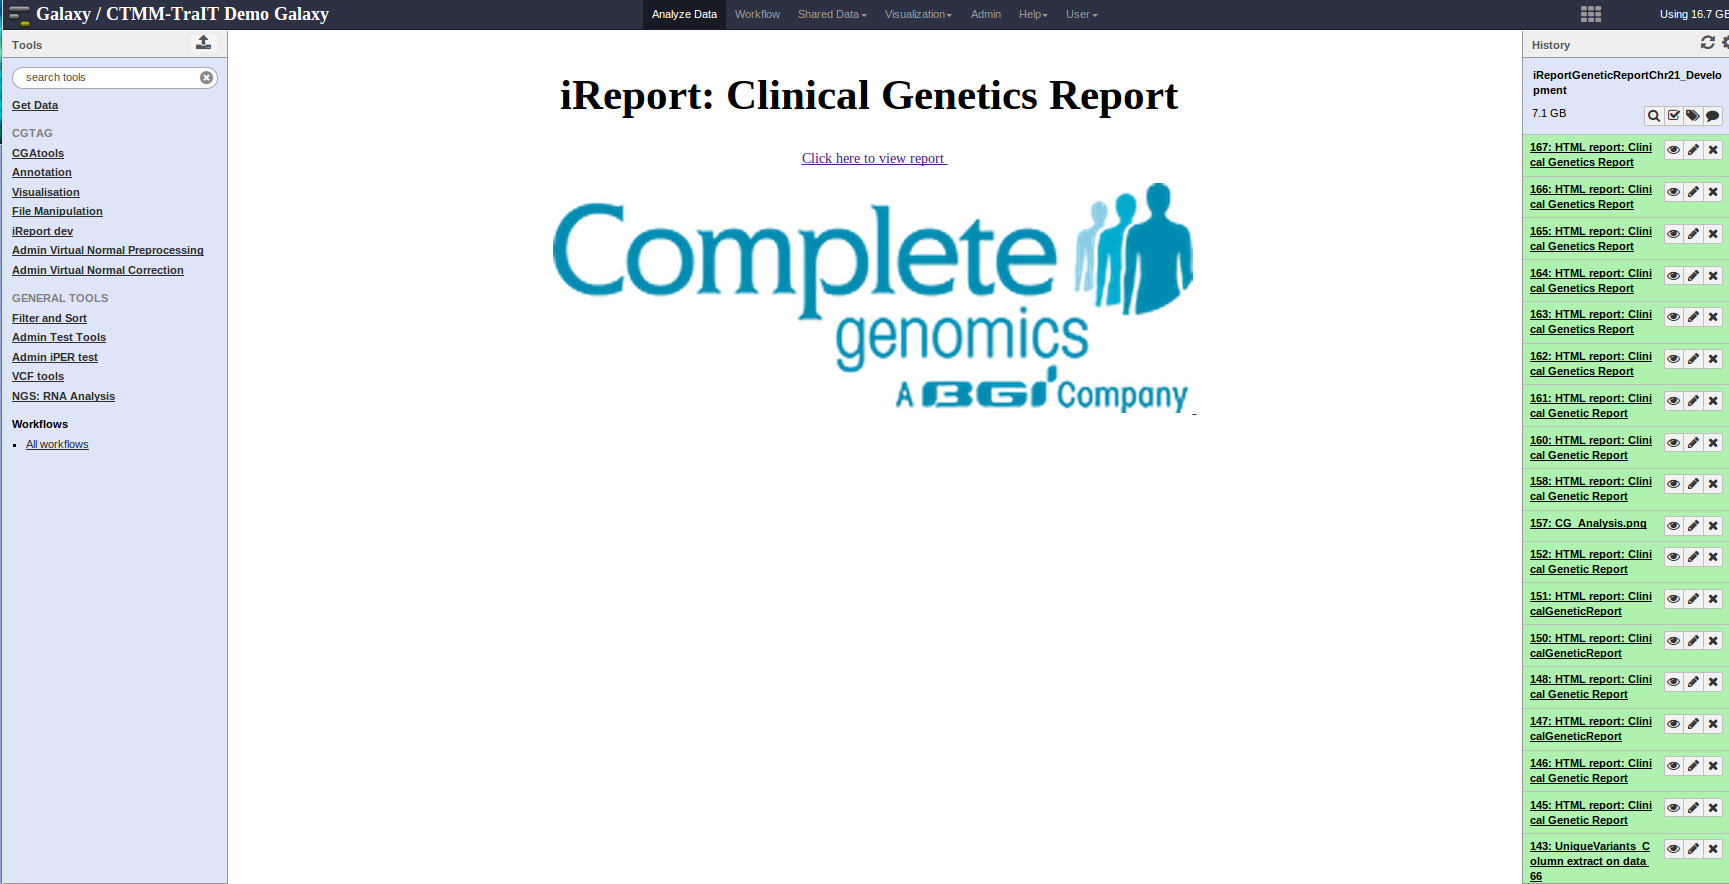
\includegraphics[scale=0.08]{chapters/images/iReport/Hiltemann_geneticreportA.jpg}   &
%    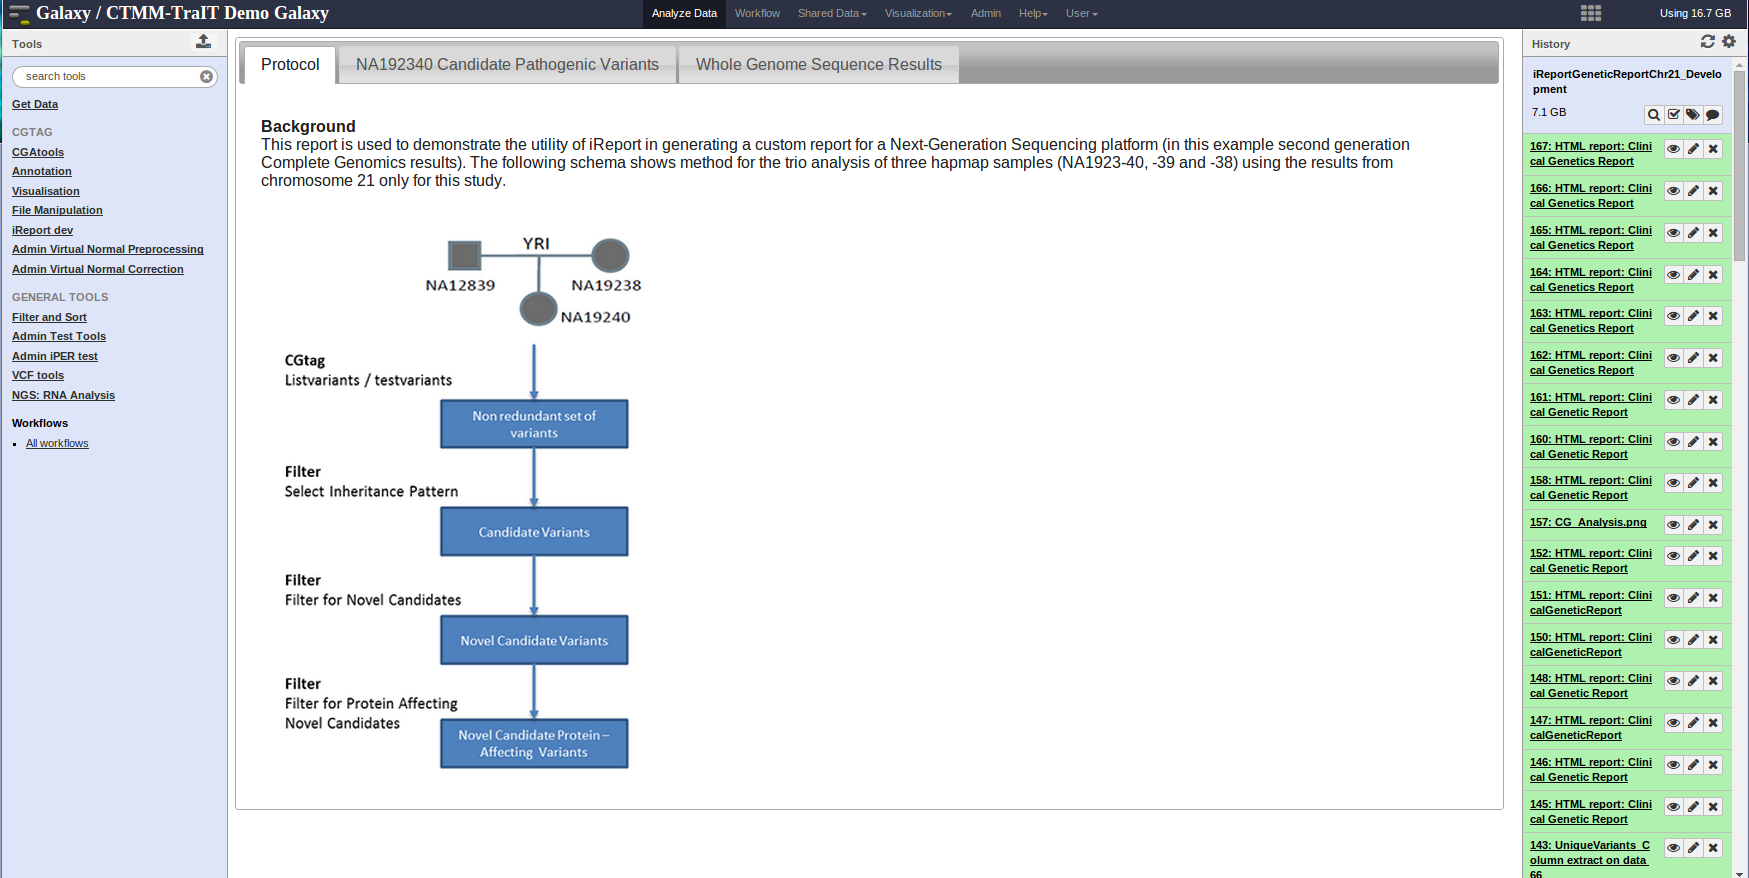
\includegraphics[scale=0.08]{chapters/images/iReport/Hiltemann_geneticreportB.jpg}   \\
%    A & B \\
%    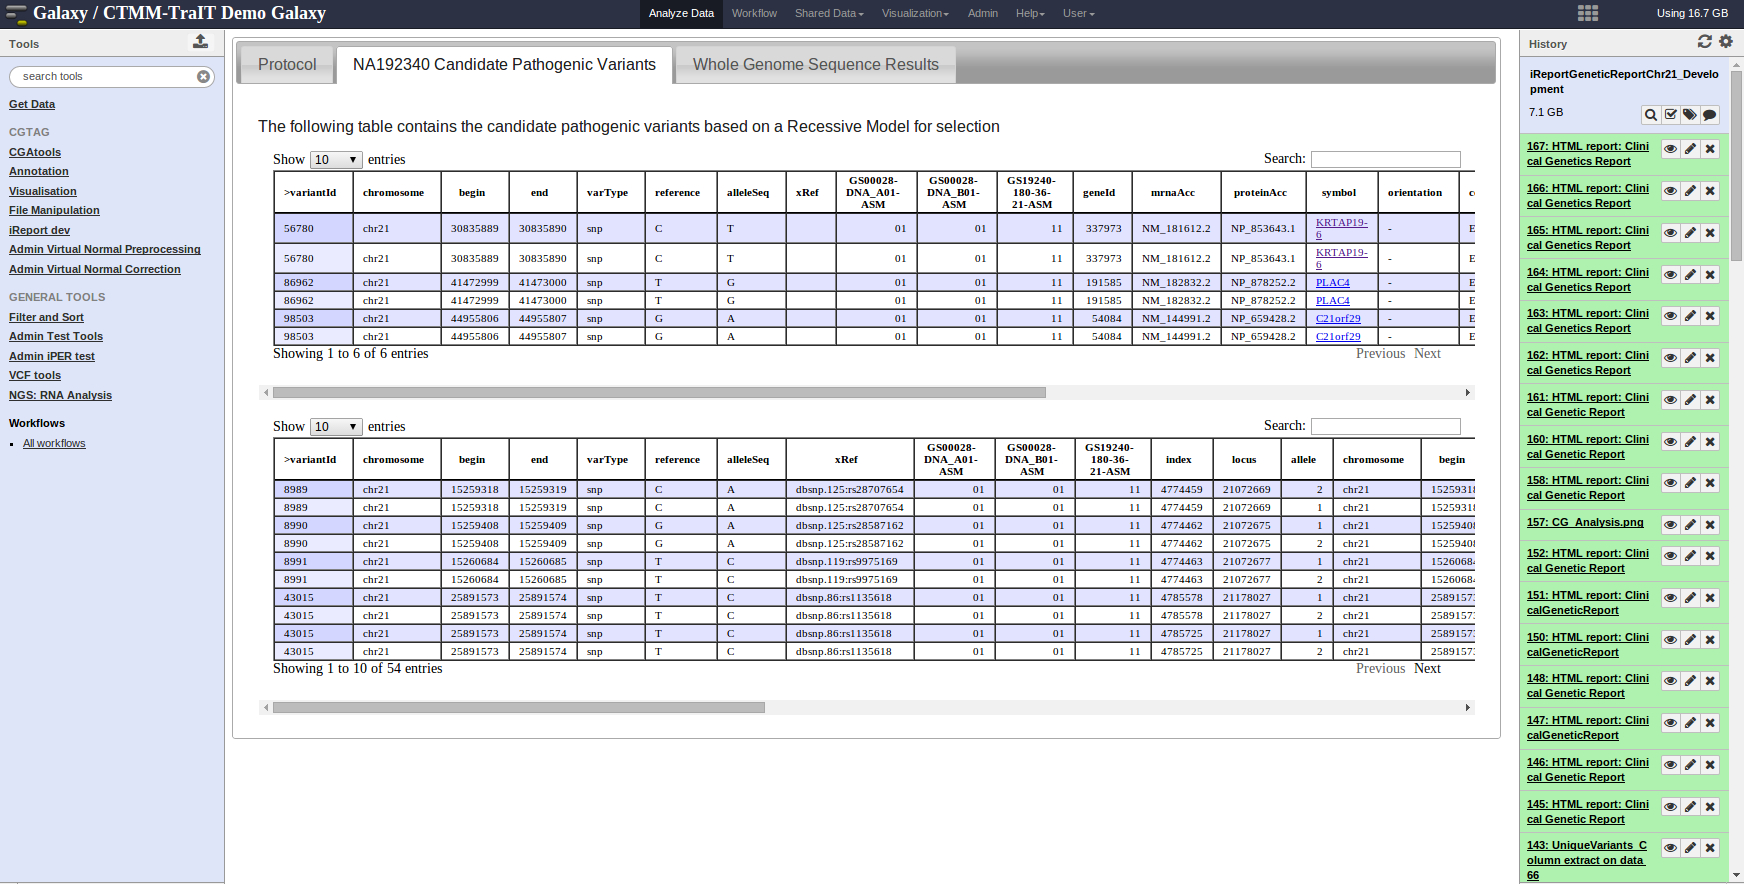
\includegraphics[scale=0.08]{chapters/images/iReport/Hiltemann_geneticreportC.jpg}   &
%    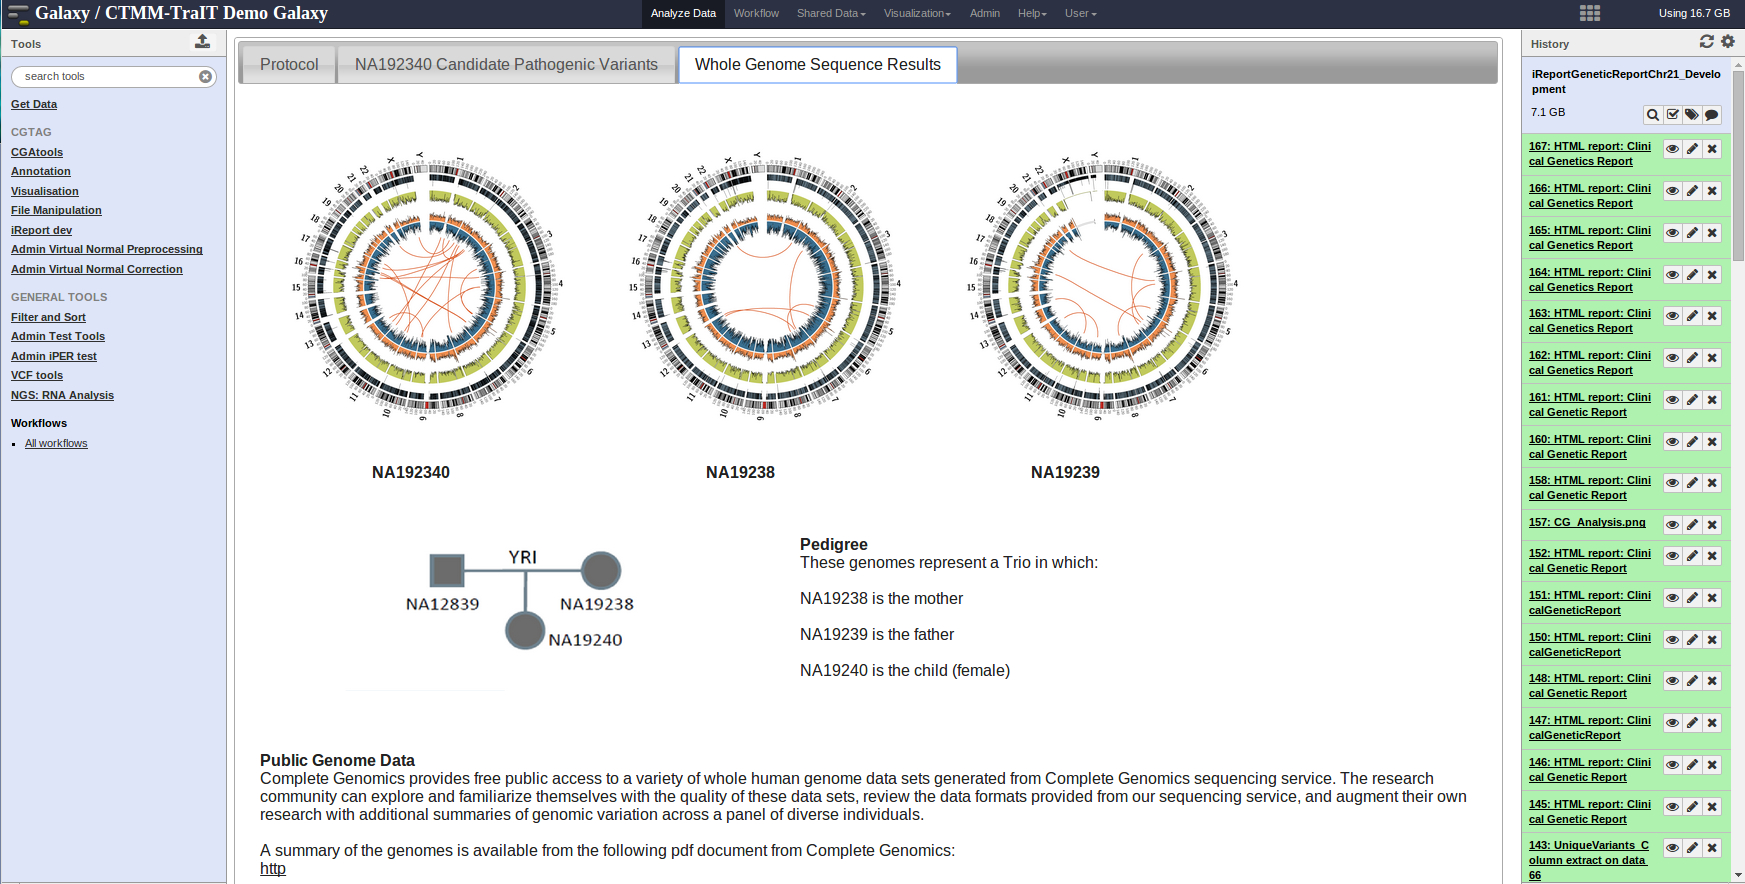
\includegraphics[scale=0.08]{chapters/images/iReport/Hiltemann_geneticreportD.jpg}   \\
%    C & D \\
%    \end{array}$
%    \end{center}
    \caption{Example iReport: Genetic Report. Example iReport for Clinical Genetics. A) Cover page with custom image. B) First tab, explaining the protocol used. C) Second tab, tables of candidate pathogenic variants, gene columns linking out to GeneCards. D) Fourth tab showing Circos images and family structure.  }
    \label{fig:trioscreenshots}
\end{figure}

\section*{Conclusions}
iReport is a easy-to-use, flexible tool for generating traceable, standardized reports which are easily shared between users within and across platforms. We have demonstrated that iReport is capable of creating a customised genetics report from results generated within Galaxy and may be shared with collaborators on the same platform, or with the public. Additionally, data or results generated externally can be uploaded into Galaxy and can also be used by iReport. These reports are generated as web pages and may be downloaded in their entirety to be easily shared across systems.

The genetics report presented here represents the bare minimal reporting that is required to summarise the output for a genetic variation analysis. Whilst we used a trio of individuals to demonstrate how to select protein-affecting candidate variants based on a recessive model, any number of model outcomes and other assay results may be included in an iReport.

We developed iReport to simplify reporting and sharing the output from \emph{omics} and non-high throughput assays analysed both in and external to Galaxy. We have also utilised iReport for more complex analysis workflows, such as summarising translational research and diagnostic applications for cancer and immunological research and diagnostics.

\section*{Availability and requirements}
Project name: iReport \\
Project home page: \url{https://github.com/shiltemann/iReport} \\
CTMM-TraIT public Galaxy instance: \url{https://galaxy.ctmm-trait.nl} \\
iReport tool shed repository: \url{https://toolshed.g2.bx.psu.edu/view/saskia-hiltemann/ireport} \\
\ \\
Operating system(s): Unix-based Operating Systems \\
Programming languages: Bash, Perl, Python \\
Other Requirements: Galaxy \\
License: GNU GPL \\
Any restrictions to use by non-academics: none \\
\ \\
Examples: \\
iReport about iReport published history:
\url{http://galaxy.ctmm-trait.nl/u/saskia-hiltemann/h/gcc2014-ireport-about-ireport}, or \url{tinyurl.com/llrzz9w} \\
Clinical Genetics iReport published history:
\url{http://galaxy.ctmm-trait.nl/u/andrew-stubbs/h/ireportgeneticreportchr21}
%Tool shed repository for iReport: https://toolshed.g2.bx.psu.edu/view/saskia-hiltemann/ireport \\
%GitHub repository: https://github.com/shiltemann/iReport \\

\section*{Availability and supporting data}
The iReport tool, user manual (published page), and example data and histories are available at the CTMM-TraIT Galaxy server~\cite{url-traitgalaxy}.

\section*{Abbreviations}
CGtag: Complete Genomics Toolkit and Annotation in a Cloud-based Galaxy. \\
CTMM-TraIT: Center for Translational Molecular Medicine - Translational IT. \\
NGS: Next Generation Sequencing. \\
URL: Uniform Resource Locator.

\section*{Acknowledgements}
 This study was performed within the framework of the Center for Translational Molecular Medicine (CTMM). TraIT project (grant 05T-401).

\footnotesize
\bibliographystyle{ieeetr}
\bibliography{references}
\normalsize

\cleartorightpage
\begin{savequote}[75mm]
"We ignore public understanding of science at our peril"
\qauthor{Eugenie Clark}
\end{savequote}

\chapter{Training}\label{chapter:training}

\begin{figure}[t!]

\includegraphics[height=10em]{frontmatter/images/chapter-header-training.png}
\end{figure}
\setcounter{figure}{-1}
\setcounter{table}{-1}
\setcounter{section}{-1}

Training is a vital component of accessible research. Galaxy enables the domain experts to perform complex analyses without needing to consult with a bioinformatician. This user-friendliness also makes Galaxy an ideal platform for training, allowing learners to focus solely on the analysis and scientific concepts, rather than the minutiae of tool installation and maintenance or the commandline interface details. To this end, we developed a central, community-driven infrastructure for Galaxy training materials, designed for ease-of-use for both trainees and instructors. Furthermore, by centralising training materials, maintenance and expansion becomes a collaborative effort supported by the global Galaxy trainer community.

This chapter contains the following sub-chapters:

\begin{enumerate}[label=\ref{chapter:training}.\arabic*]
\itemsep-0.5em
\setcounter{enumi}{-1}
\item Community-Driven Data Analysis Training for Biology
\end{enumerate}

  % reset references counter
\setcounter{NAT@ctr}{-1}

\chapter*{}

\begin{figure}[t!]
\centering

\includegraphics[height=10em]{frontmatter/images/chapter-header-training.png}
\end{figure}
\vspace{-4cm}

\articletitle{Community-driven data analysis training \\ for biology}
Bérénice Batut\textsuperscript{\ref{affil:freiburg}*},
Saskia Hiltemann\textsuperscript{\ref{affil:emc2}*},
Andrea Bagnacani\textsuperscript{\ref{affil:rostock}},
Dannon Baker\textsuperscript{\ref{affil:hopkins}},
Clemens Blank\textsuperscript{\ref{affil:freiburg}},
Anthony Bretaudeau\textsuperscript{\ref{affil:abretaud}},
Loraine Brillet-Guéguen\textsuperscript{\ref{affil:roscoff}},
Martin Čech\textsuperscript{\ref{affil:pennstate}},
John Chilton\textsuperscript{\ref{affil:pennstate}},
Dave Clements\textsuperscript{\ref{affil:hopkins}},
Olivia Doppelt-Azeroual\textsuperscript{\ref{affil:pasteur}},
Anika Erxleben\textsuperscript{\ref{affil:freiburg}},
Mallory Ann Freeberg\textsuperscript{\ref{affil:ebi}},
Simon Gladman\textsuperscript{\ref{affil:melbourne}},
Youri Hoogstrate\textsuperscript{\ref{affil:emc}},
Hans-Rudolf Hotz\textsuperscript{\ref{affil:basel}},
Torsten Houwaart\textsuperscript{\ref{affil:freiburg}},
Pratik Jagtap\textsuperscript{\ref{affil:minnesota}},
Delphine Larivière\textsuperscript{\ref{affil:pennstate}},
Gildas Le Corguillé\textsuperscript{\ref{affil:roscoff}},
Thomas Manke\textsuperscript{\ref{affil:maxplanck}},
Fabien Mareuil\textsuperscript{\ref{affil:pasteur}},
Fidel Ramírez\textsuperscript{\ref{affil:maxplanck}},
Devon Ryan\textsuperscript{\ref{affil:maxplanck}},
Florian Christoph Sigloch\textsuperscript{\ref{affil:freiburg}},
Nicola Soranzo\textsuperscript{\ref{affil:earlham}},
Joachim Wolff\textsuperscript{\ref{affil:freiburg}},
Pavankumar Videm\textsuperscript{\ref{affil:freiburg}},
Markus Wolfien\textsuperscript{\ref{affil:rostock}},
Aisanjiang Wubuli\textsuperscript{\ref{affil:leibniz}},
Dilmurat Yusuf\textsuperscript{\ref{affil:freiburg}},
Galaxy Training Network\textsuperscript{\ref{affil:gtn}},
Rolf Backofen\textsuperscript{\ref{affil:freiburg}},
Anton Nekrutenko\textsuperscript{\ref{affil:pennstate}},
Björn Grüning\textsuperscript{\ref{affil:freiburg}}

* Bérénice Batut and Saskia Hiltemann contributed equally to this work.

\textbf{Published in:} \emph{Cell Systems}, 2018 Jun 27;6(6):752-758.e1 \\
DOI: \url{https://doi.org/10.1016/j.cels.2018.05.012}

\small
\begin{enumerate}
\itemsep-0.5em
\item Albert-Ludwigs-University, Freiburg  Germany. \label{affil:freiburg}
\item Erasmus Medical Centre, Rotterdam, The Netherlands. \label{affil:emc2}
\item Department of Systems Biology and Bioinformatics, University of Rostock, Rostock, Germany. \label{affil:rostock}
\item INRA, UMR IGEPP, BIPAA/GenOuest, Campus Beaulieu, Rennes, France. \label{affil:abretaud}
\item CNRS, UMPC, FR2424, ABiMS, Station Biologique, Roscoff, France. \label{affil:roscoff}
\item The Pennsylvania State University, University Park, PA, USA. \label{affil:pennstate}
\item Johns Hopkins University, Baltimore MD USA. \label{affil:hopkins}
\item Bioinformatics and Biostatistics HUB, Centre de Bioinformatique, Biostatistique et Biologie Integrative (C3BI, USR 3756 Institut Pasteur et CNRS) – Paris, France. \label{affil:pasteur}
\item European Bioinformatics Institute, Hinxton, Cambridge, UK. \label{affil:ebi}
\item Melbourne Bioinformatics, The University of Melbourne, Australia. \label{affil:melbourne}
\item Friedrich Miescher Institute for Biomedical Research, Basel, Switzerland. \label{affil:basel}
\item Biochemistry, Molecular Biology and Biophysics, University of Minnesota Medical School, Minneapolis, USA. \label{affil:minnesota}
\item Max Planck Institute of Immunobiology and Epigenetics, Freiburg, Germany. \label{affil:maxplanck}
\item Earlham Institute, Norwich, UK. \label{affil:earlham}
\item Leibniz Institute for Farm Animal Biology (FBN), Dummerstorf, Germany. \label{affil:leibniz}
\item https://galaxyproject.org/teach/gtn/ \label{affil:gtn}


\end{enumerate}
\normalsize



\section*{Abstract}
The primary problem with the explosion of biomedical datasets is not the data itself, not computational resources, and not the required storage space, but the general lack of trained and skilled researchers to manipulate and analyze these data. Eliminating this problem requires development of comprehensive educational resources. Here we present a community-developed and driven training framework that enables modern, interactive learning of life sciences data analysis as well as facilitating easy development of tutorials. The key feature of our system is that it is not a static but a continuously improved collection of tutorials. By coupling tutorials with a web-based analysis framework, biomedical researchers can learn by performing computation themselves through a web-browser without the need to install software or search for example datasets. Our ultimate goal is to expand the breadth of training materials to include fundamental statistical and data science topics and to precipitate a complete re-engineering of undergraduate and graduate curricula in life sciences.

\section*{Introduction}
Rapid development of DNA sequencing technologies has made it possible for biomedical disciplines to rival the physical sciences in data production capability. The combined output of today’s sequencing instruments has already surpassed the data generation speed of resources such as the Large Hadron Collider and is rivaling those in the field of astronomy. Yet biology is different from physics (and other quantitative disciplines) in one fundamental aspect—the lack of computational and data analysis training in standard biomedical curricula. Many biomedical scientists do not possess the skills to use or even access existing analysis resources.
Such paucity of training also negatively impacts the ability of biomedical researchers to collaborate with their statistics and math counterparts, because of the inability to speak each other’s language. In addition, an estimated one-third of biomedical researchers do not have access to proper data analysis support~\cite{larcombe2017elixir}. The only operative way to address these deficiencies is with training. The need for such training cannot be overstated: while the majority (>95\%) of researchers work or plan to work with large datasets, most (>65\%) possess only minimal bioinformatics skills and are not comfortable with statistical analyses~\cite{larcombe2017elixir},~\cite{williams2017vision}.
This overwhelming need drives the demand, which, at present, greatly exceeds supply~\cite{attwood2017global}. In a recent survey~\cite{survey2013embl} over 60\% of biologists expressed a need for more training while only 5\% called for more computing power. Thus one can assume that the true bottleneck of the current data deluge is not storage or processing power, but the knowledge and skills to utilize existing resources.

Since 2006 our team has been pondering the question of how to enable computationally novice users to perform complex data analysis tasks. We attempted to solve this problem by creating a platform, Galaxy (\url{http://galaxyproject.org}~\cite{afgan2016galaxy}), that provides access to hundreds of tools used in a wide variety of analysis scenarios. It features a web-based user interface while automatically and transparently managing underlying computation details~\cite{afgan2016galaxy}. It can be deployed on a personal computer, heterogeneous computer clusters, as well as computation systems provided by Amazon, Microsoft, Google and other clouds such as those running OpenStack. Over the years a community has formed around this project, providing it with an ever-growing, up-to-date set of analysis tools and expanding it beyond life sciences.

These features of Galaxy attracted many biomedical researchers, making it well suited for use as a teaching platform. Here we describe a community-driven effort to build, maintain, and promote a training infrastructure designed to provide computational data analysis training to biomedical researchers worldwide. Our effort utilizes the Galaxy platform~\cite{afgan2016galaxy} to support a comprehensive training portfolio and relies on modern web-based technologies for content maintenance and delivery.

\section*{Results and Discussion}
Our goal is to develop an infrastructure that facilitates data analysis training in life sciences. At a minimum it needs to provide an interactive learning platform tuned for current datasets and research problems. It should also provide means for community-wide content creation and maintenance, and, finally, enable trainers and trainees to use the tutorials in a variety of situations such as those where reliable Internet access is not an option.

\subsection*{Interactive learning tailored to research problems}

\begin{table}{}
    \begin{tabular}{llp{8cm}}
    \hline
    \ \\
    \textbf{Topic} & \textbf{Target} & \textbf{Tutorials} \\
    \ \\
    \hline
    \ \\
    Galaxy Server administration &  Admin & Galaxy Database schema, Docker and Galaxy, Advanced customisation of a Galaxy instance \\

    Assembly &  Biol & Introduction to Genome Assembly, De Bruijn Graph Assembly, Unicycler Assembly \\

    ChIP-Seq data analysis & Biol &  Identification of the binding sites of the T-cell acute lymphocytic leukemia protein 1 (TAL1), Identification of the binding sites of the Estrogen receptor \\

    Development in Galaxy &  Dev & Contributing with GitHub, Tool development and integration into Galaxy, Tool Shed: sharing Galaxy tools, Galaxy Interactive Tours, Galaxy Interactive Environments, Visualizations: charts plugins, Galaxy Webhooks, Visualizations: generic plugins, BioBlend module, a Python library to use Galaxy API, Tool Dependencies and Conda, Tool Dependencies and Containers, Galaxy Code Architecture \\

    Epigenetics & Biol & DNA Methylation \\

    Introduction to Galaxy & Biol & Galaxy 101, From peaks to genes, Multisample Analysis, Options for using Galaxy, IGV Introduction, Getting data into Galaxy \\

    Metagenomics & Biol & 16S Microbial Analysis with Mothur, Analyses of metagenomics data - The global picture \\

    Proteomics & Biol & Protein FASTA Database Handling, Metaproteomics tutorial, Label-free versus Labelled - How to Choose Your Quantitation Method, Detection and quantitation of N-termini via N-TAILS, Peptide and Protein ID, Secretome Prediction, Peptide and Protein Quantification via Stable Isotope Labelling (SIL) \\

    Sequence Analysis & Biol & Quality Control, Mapping, Genome Annotation, RAD-Seq Reference-based data analysis, RAD-Seq de-novo data analysis, RAD-Seq to construct genetic maps \\

    Train the trainers & Inst & Creating a new tutorial - Writing content in markdown, Creating a new tutorial - Defining metadata, Creating a new tutorial - Setting up the infrastructure, Creating a new tutorial - Creating Interactive Galaxy Tours, Creating a new tutorial - Building a Docker flavor for a tutorial, Good practices to run a workshop \\

    Transcriptomics & Biol & De novo transcriptome reconstruction with RNA-seq, Reference-based RNA-seq data analysis, Differential abundance testing of small RNAs \\

    \hline
    \end{tabular}
    \caption{Topics available in the Galaxy training material website (\url{https://training.galaxyproject.org}) with their target users and available tutorials. Admin = Galaxy administrators, Biol = Biomedical researchers, Dev = Tool and software developers, Inst = Instructors and Tutorial developers. The scripts for the extraction of such information are available in GitHub (\url{https://github.com/bebatut/galaxy-training-material-stats}). This table displays content current as of 28th Sep, 2017.}
    \label{table:tutorialtable}
\end{table}

Our main result is a collection of hands-on tutorials that are designed to be interactive and are built around Galaxy. The hands-on nature of our training material implies that a trainee can have two web browser windows open side-by-side: one pointed at the current tutorial and the other at a Galaxy instance. We build most tutorials around a “research story”: a scenario inspired by a previously published manuscript or an interesting dataset (with the caveat that some more technical materials do not lend themselves to this goal). To make training comprehensive, we aim to cover major branches of biomedical big data applications such as those listed in \hyperref[table:tutorialtable]{Table~\ref*{table:tutorialtable}}.

As an example, suppose that a researcher is interested in learning about metagenomic data analyses. The category “Metagenomics” at  \url{https://training.galaxyproject.org} presently contains a set of introductory slides, two hands-on tutorials (\hyperref[fig:metagenomics]{Fig.~\ref{fig:metagenomics}A}), and HTML-based slides designed as a brief (10 - 20 min) introduction to the subject. In addition, every hands-on tutorial begins with background information (\hyperref[fig:metagenomics]{Fig.~\ref{fig:metagenomics}B}) and explains how it influences data analysis. This background story is included to account for situations when tutorials are used for self-teaching in the absence of an instructor who would provide a formal introduction. After the introduction, the hands-on part of the tutorial begins and is laid out in a step-by-step fashion with explanations (boxes on \hyperref[fig:metagenomics]{Figure~\ref{fig:metagenomics}D}) of what is being done inside Galaxy, which parameters are critical, and how modifying parameters affects downstream results. The first step in this progression is usually a description of the datasets and how to obtain them. We invested a large effort in creating appropriate datasets by downsampling original published data, which is necessary since real-world datasets are usually too big for tutorials. Our goal was to make datasets as small as possible while still producing an interpretable result. We use Zenodo (\url{http://www.zenodo.org}), an open data archiving and distribution platform, to store the tutorial datasets and to provide them with stable digital object identifiers (DOIs) that can be used to credit their authors and for citation purposes.

\begin{figure}[t!]
    \centering
    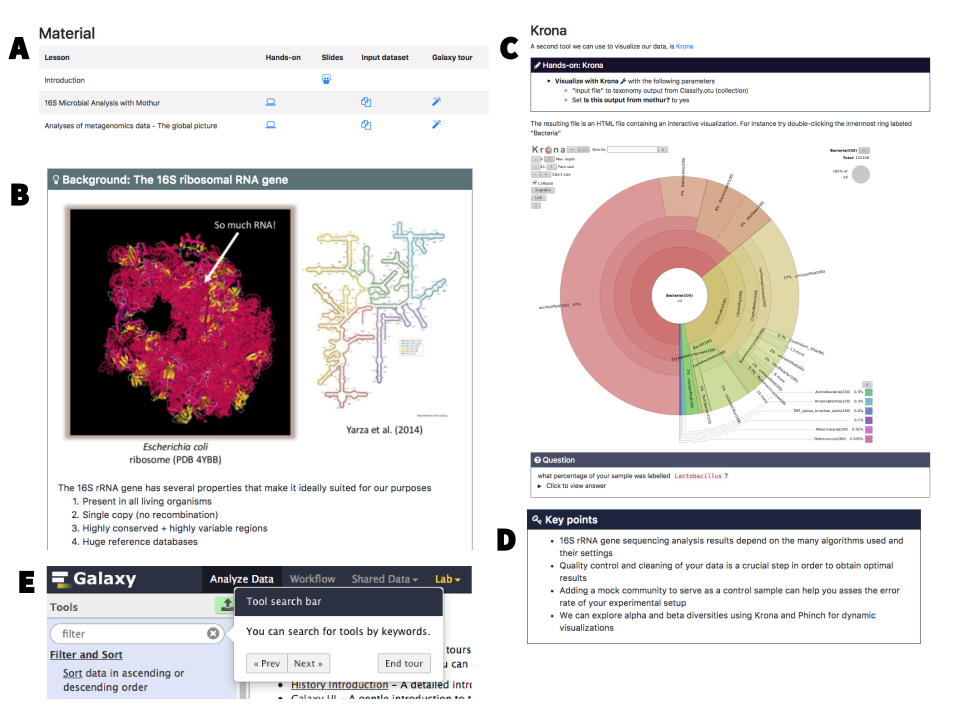
\includegraphics[width=\textwidth]{chapters/images/training/training-figure-metagenomics.png}
    \caption{Key elements of an interactive tutorial. \textbf{A.} A list of tutorials dedicated to Metagenomics. There is a set of introductory slides and two hands-on tutorials. \textbf{B.} A fragment of introductory material within a tutorial. \textbf{C.} A “hands-on” element with upper box contains instructions for running a tool inside Galaxy and shown example output of Krona tool. The question box at the bottom contains togglable answer field. \textbf{D.} Summary of key points for this tutorial displayed on the bottom of the tutorial. \textbf{E.} Fragment of Galaxy interface showing interactive tour balloon.  }
    \label{fig:metagenomics}
\end{figure}

Tutorials start with a list of prerequisites (typically other tutorials within the site) to account for the variation in trainees’ backgrounds, a rough time estimate, questions addressed during the tutorial, learning objectives, and key points (e.g., \hyperref[fig:metagenomics]{Fig.~\ref{fig:metagenomics}D}). These components help trainees and instructors to keep track of the training goals. For example, the learning objectives are single sentences describing what a trainee will be able to do as a result of the training~\cite{via2013best}. Throughout the tutorials, question boxes (\hyperref[fig:metagenomics]{Fig.~\ref{fig:metagenomics}C}) are added as an effective way to motivate the trainees~\cite{dollar2007enhancing}~\cite{scheines2005replacing} and guide self-training. The training material is distributed under a CC BY 4.0 (\url{https://creativecommons.org/licenses/by/4.0/}) license: its contents can be shared and adapted as long as appropriate credit is given. Efforts have been made also in the direction of ensuring website accessibility to disabled persons by regular evaluation with WAVE (\url{http://wave.webaim.org}), a web accessibility evaluation tool, and by automatic checking for alternative text for the images.

Keeping trainees engaged is critical, particularly for self-training. To this end, we aim to provide interactive tours for each tutorial: using instruction bubbles (\hyperref[fig:metagenomics]{Fig.~\ref{fig:metagenomics}E}), each tutorial step can be “played” directly inside Galaxy, guiding learners to the needed tools while also allowing exploration of the framework’s functionalities.


\subsection*{Infrastructure to facilitate community-led content development}

\begin{figure}[t!]
    \centering
    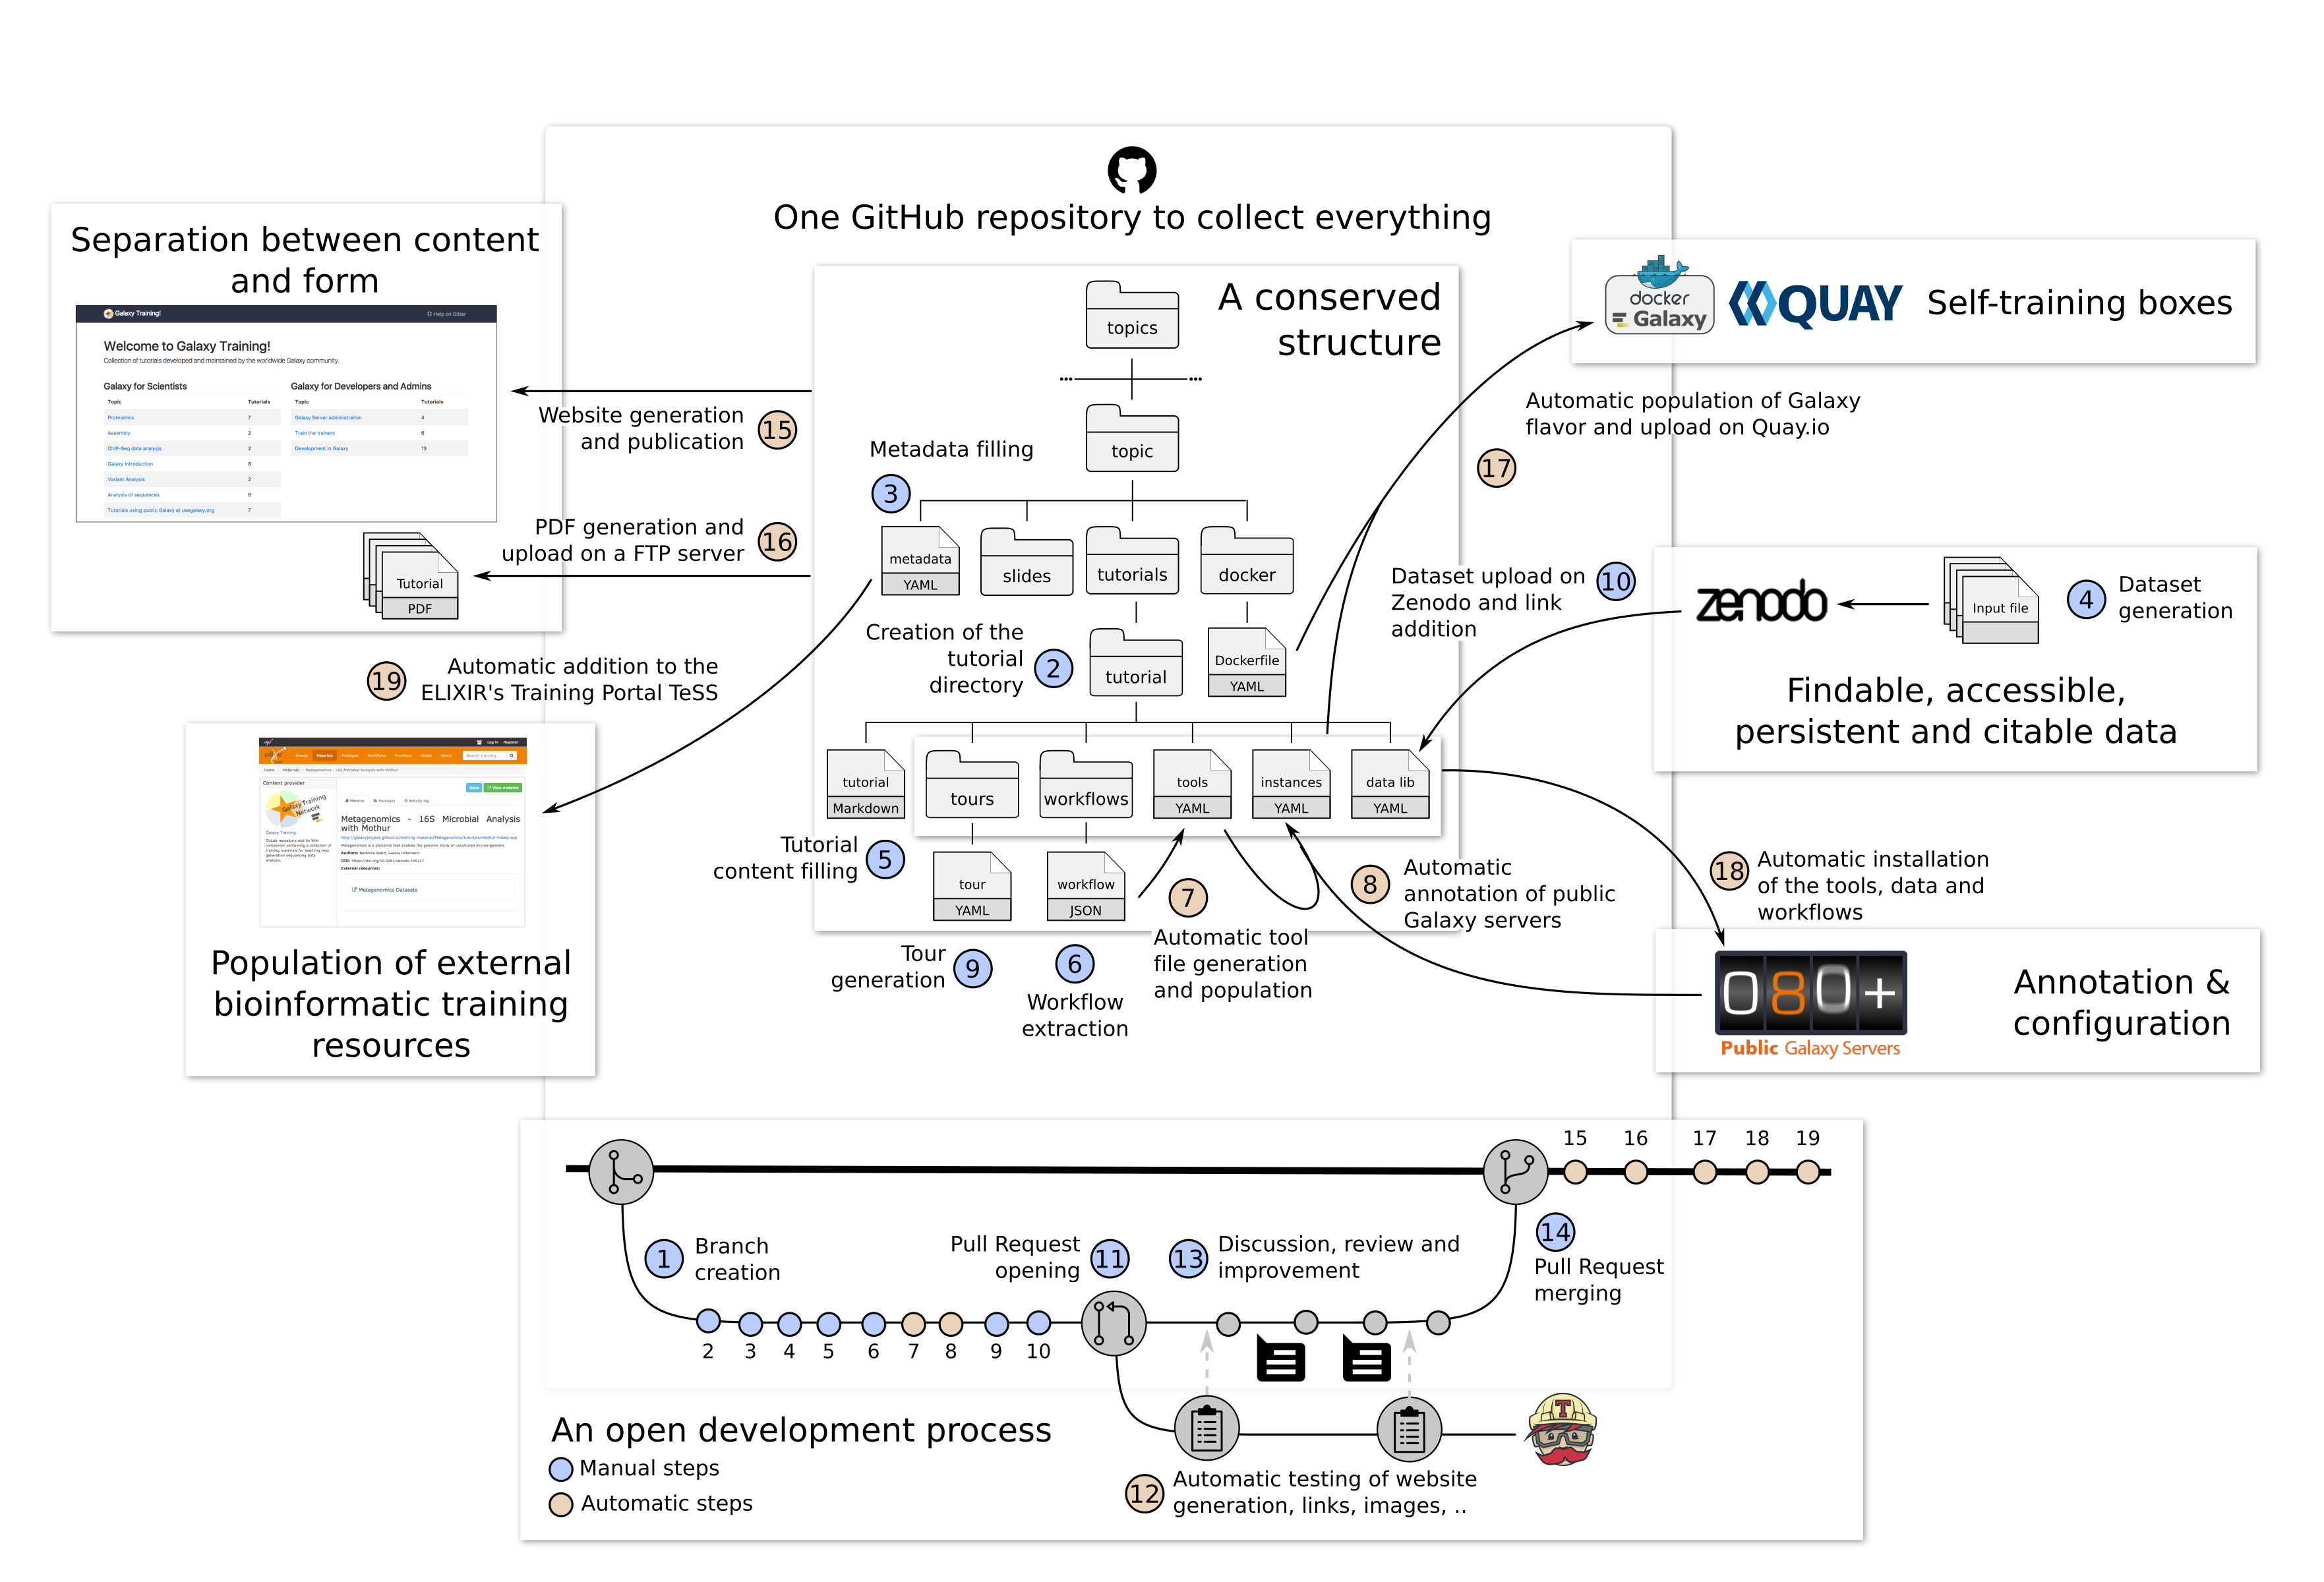
\includegraphics[width=\textwidth]{chapters/images/training/training-figure-development.png}
    \caption{Structure and development of content in GitHub (http://github.com/galaxyproject/training-material). The material is organized in different topics, each topic in a dedicated directory. Inside each topic’s directory, the structure is the same: a metadata file, a directory with the topic introduction slide decks, a directory with the tutorials and a directory with the Dockerfile describing the details to build a container for the topic that would contain a dedicated Galaxy instance with all tools relevant for the tutorials. Inside the topic directory, each tutorial related to the topic has its own subdirectory with several files: a tutorial file written in Markdown with hands-on, an optional slides file to support the tutorial, a directory with Galaxy Interactive Tours to reproduce the tutorial, a directory with workflows extracted from the tutorial, a file with the links to the input data needed for the tutorial and a file with the description of needed tools to run the tutorial. The process of development of new content is shown at the bottom of the figure.}
    \label{fig:development}
\end{figure}

To build a comprehensive collection of training materials covering the spectrum of topics in the life sciences, we must leverage community expertise, as no single group can possibly “know it all”. To achieve this goal, we built an infrastructure that makes tutorial creation a convenient, hassle-free process and enables transparent peer-review and curation to guarantee high-quality and current content. In implementing these requirements, we took inspiration from the Software and Data Carpentry~\cite{wilson2014software} projects (SDC). In SDC, materials are openly reviewed and iteratively developed on GitHub (\url{https://github.com/}) to capture the breadth of community expertise. SDC delivers training via online tutorials with hands-on sections, which offer better training support than videos because trainees who are actively participating learn more~\cite{dollar2007enhancing}.
This format is also adapted to face-to-face courses and self-training, as the content is openly accessible online. The content of these web pages is easy to edit, thus reducing the contribution barrier. The tutorials are developed in Markdown, a plain text markup language, which is automatically transformed into web-browser accessible pages. Using these strategies, we created a GitHub repository (\url{https://github.com/galaxyproject/training-material}) to collect, manage, and distribute training materials.
The architecture of this infrastructure is shown in \hyperref[fig:development]{Fig.~\ref{fig:development}} (center), with the process for developing a tutorial illustrated at the bottom of the figure. To create a new tutorial, the main repository is forked (duplicated into a user-controlled space) within GitHub by an individual developing the tutorial. The developer then proceeds to write the content using Markdown as explained in our guide at \url{https://training.galaxyproject.org/topics/training} (itself consisting of several tutorials). The guide contains detailed information on technical and stylistic aspects of tutorial development.
After settling on a final version of the tutorial (circles 1 through 10, the bottom of \hyperref[fig:development]{Fig.~\ref{fig:development}}), a pull request is created against the original repository. When a new pull request is issued, this is an indication that a new tutorial is ready to be reviewed by the editorial team. The team then makes suggestions on the new contents, these suggestions are discussed, and the content is edited accordingly. A decision is then made whether to accept the pull request. At the same time the pull request is first created, the newly added content is automatically tested for HTML generation and all links and images are verified. When the pull request is accepted, the new tutorial becomes a part of the official training material portfolio, and the entire site is regenerated.

This infrastructure has been developed in accordance with the FAIR (Findable, Accessible, Interoperable, Reusable) principles~\cite{wilkinson2016fair}. Each tutorial, slide deck, and topic is complemented by numerous metadata described in a standard, accessible, interoperable format (YAML; \url{http://yaml.org/}). The metadata is used to automatically populate the TeSS training portal at the European life-sciences Infrastructure for biological Information (ELIXIR; \url{https://tess.elixir-europe.org}), ensuring global reach~\cite{tess2016}. Each topic, tutorial, and slide deck has as metadata a reference to a topic in the EDAM ontology~\cite{ison2013edam}, a comprehensive catalog of well-established, familiar concepts that are prevalent within bioinformatics and computational biology. These references can be used to represent relationships among the materials and make them more findable and searchable.

\begin{figure}[t!]
    \centering
    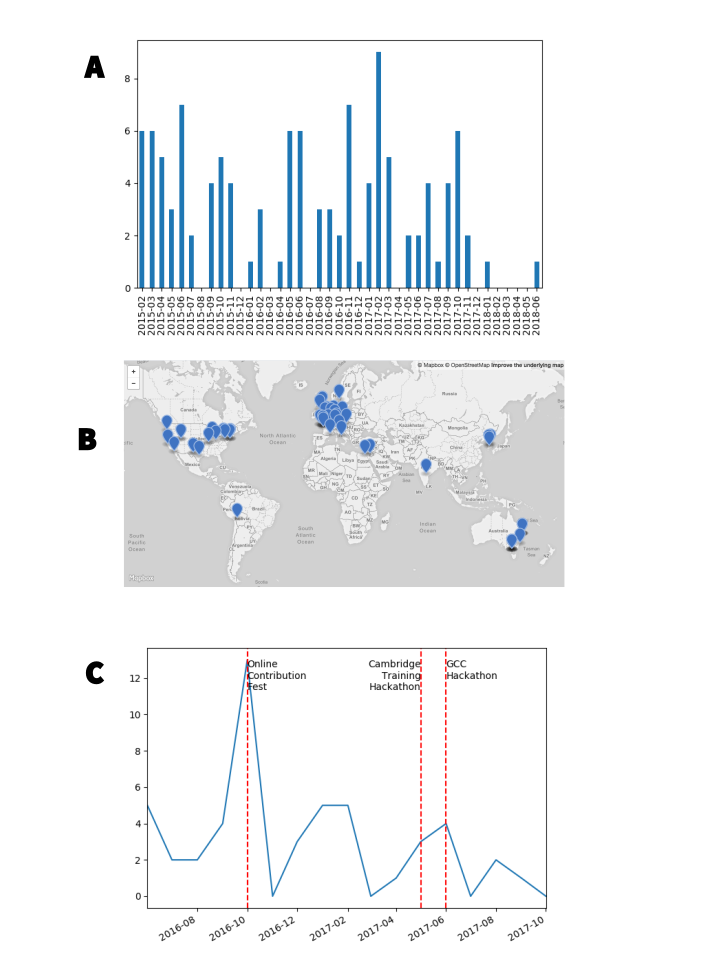
\includegraphics[width=400pt]{chapters/images/training/training-figure-stats.png}
    \caption{History of training activities. Number (A) and location (B) of registered training events organized by the Galaxy Training Network since 2015. C. Number of tutorial contributors per month.}
    \label{fig:stats}
\end{figure}

Using the framework described above, we relaunched the Galaxy Training Network (GTN; \url{https://galaxyproject.org/teach/gtn}). This growing network currently consists of 33 scientific groups (\url{https://galaxyproject.org/teach/trainers}) invested in Galaxy-based training. The GTN regularly organizes training events worldwide (\hyperref[fig:stats]{Fig.~\ref{fig:stats}}) and offers best practices for developing Galaxy-based training material, advice on compute platform choice to use for training, and a catalog of existing training resources for Galaxy (\hyperref[table:tutorialtable]{Table~\ref{table:tutorialtable}}).

\subsection*{Ensuring accessibility of tutorials}
Most training materials hosted within the GTN resource are intended to be used side-by-side with the Galaxy framework. However, the public Galaxy instances (e.g. \url{https://usegalaxy.org} or \url{https://galaxy.uni-freiburg.de}) are occasionally subject to unpredictable load, may be inaccessible due to network problems in remote parts of the world or may not have all the tools necessary for completing the tutorials. To account for these situations, we have developed a Docker-based framework for creating portable, on-demand Galaxy instances specifically targeted for a given tutorial. Docker (\url{https://www.docker.com}) is a container platform which provides lightweight virtualization by executing "images" (files that include everything needed to run a piece of software) isolated from the host computer environment. An individual creating a new tutorial lists all tools that are required to complete it in a dedicated configuration file (tools file, \hyperref[fig:development]{Fig.~\ref{fig:development}}). For example, a metagenomics tutorial uses the mothur~\cite{schloss2009introducing} set of tools as well as visualization applications such as Krona~\cite{ondov2015krona}. The corresponding Galaxy tools are listed in a configuration file that is a part of the metagenomics tutorial. This file is used to install these Galaxy tools and their dependencies into a base Galaxy Docker image (containing essential Galaxy functionality and a core set of tools) to create a dedicated “on-demand” Galaxy instance which can then be used on any trainer’s or trainee’s computer. The Docker image also contains input data, tours, workflows.

\section*{A vision for the future}
Life sciences are on a trajectory towards becoming an entirely data-driven scientific domain. A growing understanding that biomedical curricula must be modernized to reflect these changes is gaining attention~\cite{10.7554/eLife.32715}. Our project represents one of the first fully open, “grass-roots” attempts at unifying and standardizing heterogeneous training resources around the Galaxy platform. While it may not be appropriate to all, our multi-year experience with teaching workshops at various skill-levels can be summarized as the following set of recommendations, which we use as guiding principles. These recommendations may also be useful for the development of alternative frameworks as well as for curriculum planning:

\begin{enumerate}
\item \textbf{Require quantitative training.} No one expects biomedical researchers to rival their colleagues in departments of mathematics or statistics. However, background level statistical reasoning must be included in all training materials and general statistical courses must become a part of undergraduate and graduate education. This would have an enormous positive impact on the quality of biomedical research because researchers with basic understanding of quantitative concepts will not, for example, perform an RNAseq experiment without a sufficient number of replicates.
\item \textbf{Demystify computational methodologies.} Fundamental principles, limitations, and assumptions of molecular experimental techniques are typically well understood by biomedical researchers even when proprietary reagent kits are used. This is not the case with software tools, which are often treated as black boxes. We argue that fundamental principles of bioinformatic techniques (e.g., read mapping, read assembly) must be understood by experimentalists as this will also lead to an increase in overall quality of research output.
\item \textbf{Advocate the fundamental virtues of open and transparent research.} Open and transparent data analysis (e.g., through the use of open-source software) promotes replication and validation of results by independent investigators. It also speeds up research progress by facilitating reuse and repurposing of published analyses to different datasets or even to other disciplines. We advocate openness as a basic principle for computational analysis of biomedical data.
\end{enumerate}

The infrastructure presented here has been developed to support training using Galaxy, a powerful tool for teaching bioinformatics concepts and analysis. But such a model is not only limited to Galaxy. It could be applied to bioinformatics training more generally (and to other disciplines as well) to support learners and instructors in this ever-changing landscape that is the life sciences.


\section*{Acknowledgments}
The authors are grateful to the Freiburg Galaxy and Core Galaxy teams, as without these resources this work would not be possible. Adoption of Galaxy Tours has been accelerated with the introduction of Galaxy Tour Builder (\url{https://zenodo.org/record/830481}) by William Durand (\url{https://tailordev.fr}). This project was supported by Collaborative Research Centre 992 Medical Epigenetics (DFG grant SFB 992/1 2012), German Federal Ministry of Education and Research (BMBF grant 031 A538A RBC (de.NBI)), NIH Grants U41 HG006620 and R01 AI134384-01, as well as NSF Grant 1661497.
References


\bibliographystyle{ieeetr}
\bibliography{references}

\cleartorightpage
\begin{savequote}[75mm]
“As always in life, people want a simple answer \. \. \. and it’s always wrong.”
\qauthor{Susan Greenfield}
\end{savequote}

\chapter{Fusion Gene Detection}\label{chapter:fusiongenes}
\setcounter{figure}{-1}
\setcounter{table}{-1}
\setcounter{section}{-1}

\begin{figure}[t!]
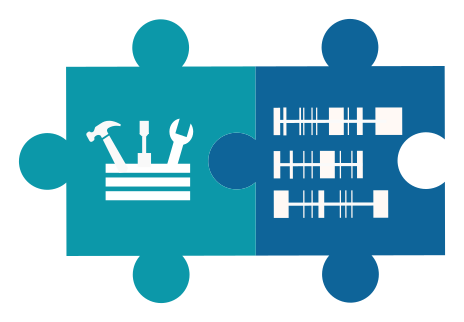
\includegraphics[height=10em]{frontmatter/images/chapter-header-fusion-tools.png}
\end{figure}
\setcounter{figure}{-1}
\setcounter{table}{-1}
\setcounter{section}{-1}


Structural variations are large-scale rearrangements of the genome. When these alterations occur within genes, novel hybrid genes called \emph{fusion genes} may be formed. Accurate detection of SVs and resulting fusion genes are an informative in cancer research studies.

We created iFUSE, web-based application to visualize and explore structural variants, and identify and prioritize potential fusion genes within a sample. We subsequently used this tool to detect multiple fusions in VCaP cell line. Futhermore, we were discovered chromothirpsis on chromosome 5q of this sample, and used the Circos tool to visualize this in a single plot.

This chapter contains the following sub-chapters:

\begin{enumerate}[label=\ref{chapter:fusiongenes}.\arabic*]
\itemsep-0.5em
\setcounter{enumi}{-1}
\item \textbf{iFUSE:} integrated fusion gene explorer
\item Gene fusions by chromothripsis of chromosome 5q in the VCaP prostate cancer cell line
\end{enumerate}

  % reset references counter
\setcounter{NAT@ctr}{-1}

\phantomsection
\addcontentsline{toc}{section}{The Informatics: iFUSE}
\articletitle{iFUSE: integrated fusion gene explorer}
Saskia Hiltemann \textsuperscript{1}, Elizabeth A. McClellan\textsuperscript{2}, Jos van Nijnatten\textsuperscript{2}, Sebastiaan Horsman\textsuperscript{2}, Ivo Palli\textsuperscript{2}, Ines Teles Alves\textsuperscript{1,3}, Thomas Hartjes\textsuperscript{1}, Jan Trapman\textsuperscript{3}, Peter van der Spek\textsuperscript{2}, Guido Jenster\textsuperscript{1}, and Andrew Stubbs\textsuperscript{2}

\small
\begin{enumerate}
\itemsep-0.5em
\item Department of Urology, Erasmus MC, 3015 GE Rotterdam, The Netherlands.
\item Department of Bioinformatics, Erasmus MC, 3015 GE Rotterdam, The Netherlands.
\item Department of Pathology, Erasmus MC, 3015 GE Rotterdam, The Netherlands.
\end{enumerate}

Published in: Bioinformatics \\
DOI: \url{10.1093/bioinformatics/btt252} \\

\section*{Abstract}

\textbf{Summary:} We present iFUSE (integrated FUSion gene Explorer), an online visualization tool that provides a fast and informative view of structural variation data and prioritizes those breaks likely representing fusion genes. \color{black} This application uses calculated breakpoints to determine fusion genes based on the latest annotation for genomic sequence information, and where relevant the structural variation (SV) events are annotated with predicted RNA and protein sequences. iFUSE takes as input either a Complete Genomics (CG) junction file, a FusionMap \cite{ge2011fusionmap} fusion detection report file, or a file already analysed and annotated by the iFUSE application on a previous occasion. \\
\textbf{Results:} We demonstrate the utility of iFUSE with case studies from tumour-normal SV detection derived from Complete Genomics whole-genome sequencing results. \\
\textbf{Availability:} iFUSE is available as a web service at \url{http://ifuse.erasmusmc.nl}


\section*{Introduction}

Structural variation analysis is a common requirement in the study of cancer where many fusion genes have been implicated in the progression of cancer \cite{mitelman2007impact, kumar2008recurrent}
The use of next-generation sequencing for fusion gene detection in cancer \cite{edgren2011identification, ge2011fusionmap, mcpherson2011defuse}, structural variation in non-cancerous diseases \cite{sanders2011multiple, levy2011rare} and in normal genomes \cite{10002010map} has expanded knowledge of the importance of these events.
In a recent study the use of \textit{de novo} assembly in association with SV detection suggests that SVs account for more diversity between individuals than do single nucleotide polymorphisms (SNPs) \cite{li2011structural}. Complete Genomics uses \textit{de novo} assembly during SV, single nucleotide variation (SNV) and copy number variation (CNV) determination \cite{carnevali2012computational}.

Traditionally, for a given SV, a user can visualize the individual (sides of the) breaks in viewers such as IGV \cite{thorvaldsdottir2013integrative,robinson2011integrative}, but not the resulting event or fusion gene as a whole, and must manually retrieve the sequence of the resulting event based on the exons from both genes of the proposed fusion gene and determine the orientation and frame of the predicted transcript and encoded polypeptide sequences. Other applications also offer visualisation, but with the caveat that the user must process their data within the application, e.g inGAP-SV \cite{qi2011ingap}, or that a bioinformatician is required to render the visualization using e.g. Circos \cite{krzywinski2009circos}. Our aim is to deliver a web-based application that allows scientists to visualize all detected SV events and fusion genes determined in their results and to provide the concomitant candidate transcripts and polypeptide sequences associated with the detected fusion genes (\hyperref[fig:screenshot]{Figure \ref*{fig:screenshot}}). No other application exists at the moment to categorize and visualize the candidate fusion genes, and determine the proposed sequence for gDNA, RNA and polypeptides from standard SV files.

\begin{figure}
\centerline{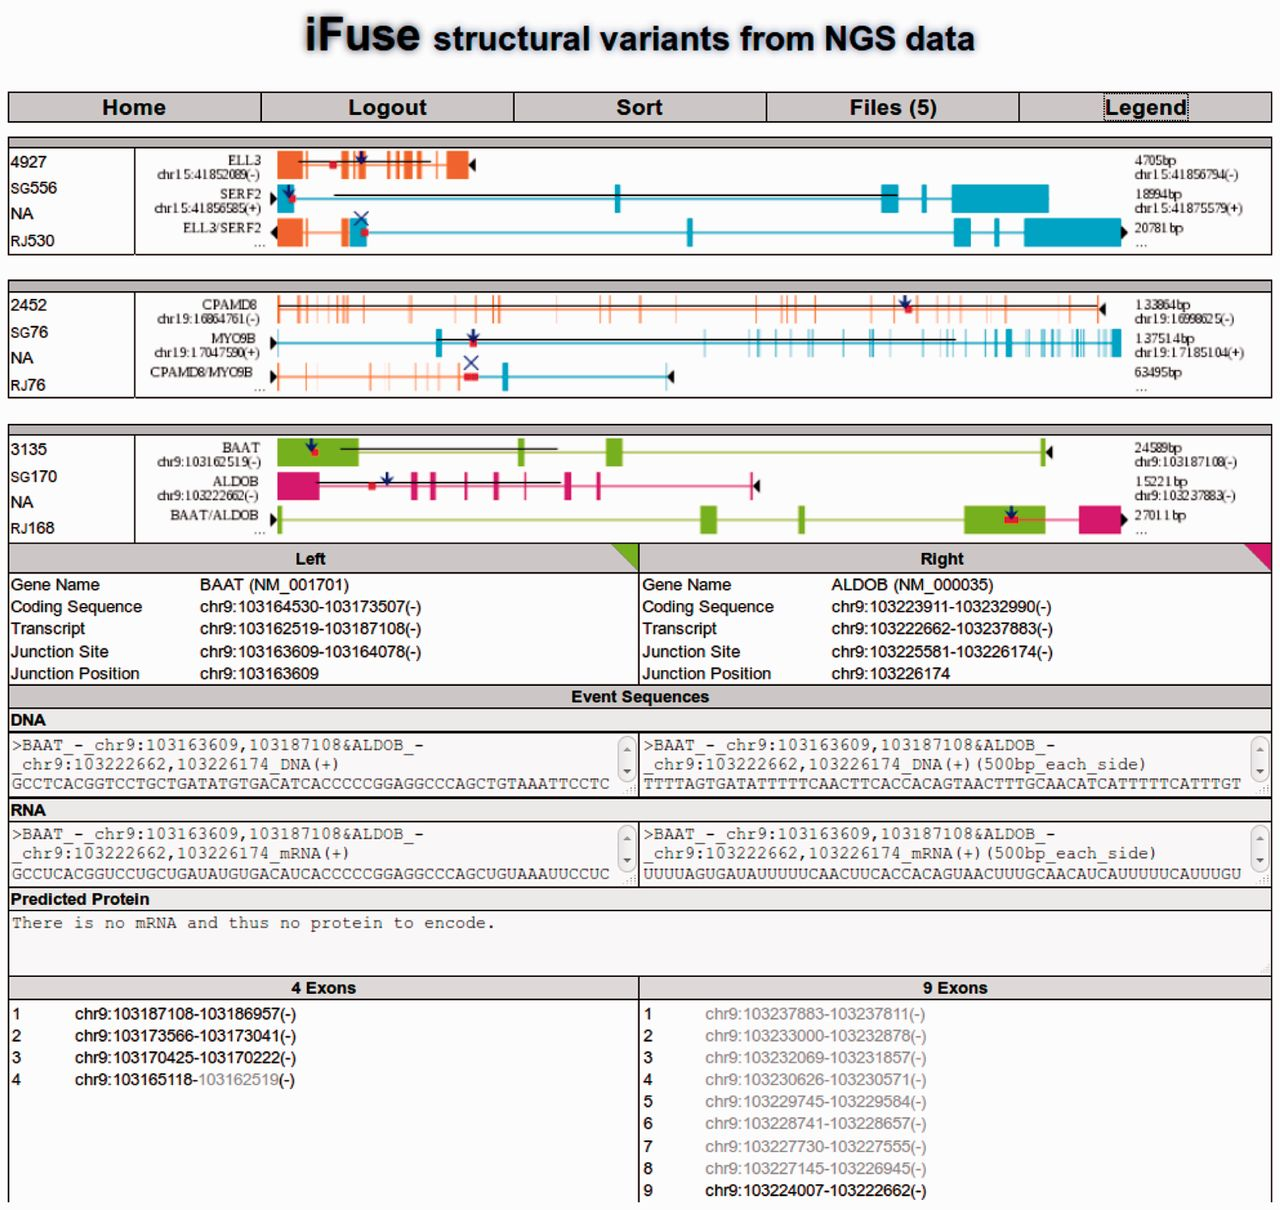
\includegraphics[width=250pt]{chapters/images/iFUSE/ifusess.jpeg}}
\caption{Screenshot of iFUSE. SVs are visualised and where applicable, the predicted DNA, RNA and protein sequences are reported.}
\label{fig:screenshot}
\end{figure}


\section*{Methods}

iFUSE is a PHP-coded application running on an Apache web server with a mySQL database for user management and R for data analysis. Gene-based feature annotation is provided using the UCSC gene tables (hg18 and hg19). Documentation details, including full application configuration, are available from the website (\href{http://ifuse.erasmusmc.nl}{http://ifuse.erasmusmc.nl}).

iFUSE takes as input either a Complete Genomics (CG) junctions file or a fusion detection report as generated by the FusionMap tool \cite{ge2011fusionmap}.  To perform a comparison of two or more genomes, the Complete Genomics tool Junctions2Events can be used prior to visualisation within iFUSE.\color{black}
The input file is validated and then analyzed using R, after which a graphical representation for each event is generated. This representation displays the promotor, introns, exons and the junction site, and additional information including DNA, RNA and protein sequences are presented to the user. These events can be filtered and sorted by the user, either using general properties or by zooming in on a single event and filtering for nearby junctions or events with similar properties.

The input files uploaded to iFUSE are annotated in R using information retrieved from UCSC gene tables and the input files. The resulting output file can be retrieved from iFUSE for manual inspection, and can also be used directly as input to iFUSE.

Example input files can be downloaded from the downloads section of the iFUSE website and users can test the application without registration by selecting the option to start an anonymous session. Any files uploaded by the user will be deleted at the end of the anonymous session.

iFUSE accounts are password protected, the application has been tested for security risks such as SQL injections, and our servers undergo periodical CERT vulnerability scans (http://www.cert.org). Furthermore, when a user deletes a file via the iFUSE web interface, it is purged completely from our systems.

\section*{Discussion}


Two public cancer genomes have been used to demonstrate the utility of iFUSE for the prediction of fusion genes. Genomes were downloaded from Complete Genomics (\href{ftp2.completegenomics.com}{ftp2.completegenomics.com}). The results can be found in \hyperref[tab:results]{Table \ref*{tab:results}}.


\begin{table}[!t]
    \begin{tabular}{lcccc}
        \toprule
                              & S1 Tumour  & S1 Normal  & S2 Tumour   & S2 Normal \\
        \midrule
        HG18                  &            &            &             &         \\
        Junctions             & 1579       & 1594       & 1558        & 1387    \\
        Genes on both sides   & 32         & 15         & 23          & 4       \\
        Same orientation      & 21         & 14         & 16          & 1       \\
                              &            &            &             &         \\
        HG19                  &            &            &             &         \\
        Junctions             & 1581       & 1592       & 1559        & 1390    \\
        Genes on both sides   & 21         & 12         & 31          & 7       \\
        Same orientation      & 10         & 6          & 17          & 3       \\
        \toprule
    \end{tabular}
    \caption{Results from iFUSE on public datasets. Sample 1 (S1): HCC1187, Sample 2 (S2): HCC2218, public datasets downloadable from Complete Genomics. (ftp://ftp2.completegenomics.com/Cancer\_pairs/)
    }
    \label{tab:results}
\end{table}

An event is labeled as a fusion gene if the breakpoint has two different genes on either side. If the two sides also have the same orientation (are on the same strand, or in the case of an inversion on opposite strands) and are also in frame, the event is called a fusion protein.

\section*{Conclusion}

iFUSE provides scientists with a convenient method to visualize, categorize, and filter structural variation analysis output using Complete Genomics junction files or the FusionMap fusion detection report files as input to the application.

\section*{Acknowledgements}

This study was performed within the framework of CTMM, the Center for Translational Molecular Medicine. TraIT project (grant 05T-401).

We would like to thank Rick Tearle and Steve Lincoln from Complete Genomics whose valuable discussions on Complete Genomics analysis methods supported our application development.


\bibliographystyle{ieeetr}
\bibliography{references}

  %\setcounter{figure}{-1}
%\setcounter{table}{-1}
%\setcounter{section}{-1}
\setcounter{NAT@ctr}{-1}
\phantomsection\addcontentsline{toc}{section}{The Bio: VCaP Chromothripsis}
\articletitle{Gene fusions by chromothripsis of chromo- some 5q in the VCaP prostate cancer cell line}
Inês Teles Alves\textsuperscript{\ref{affil:emc-urology},\ref{affil:emc-pathology},*},
Saskia Hiltemann\textsuperscript{\ref{affil:emc-bioinf},\ref{affil:emc-urology},*},
Thomas Hartjes\textsuperscript{\ref{affil:emc-urology}},
Peter van der Spek\textsuperscript{\ref{affil:emc-bioinf}},
Andrew Stubbs\textsuperscript{\ref{affil:emc-bioinf}},
Jan Trapman\textsuperscript{\ref{affil:emc-pathology}},
Guido Jenster\textsuperscript{\ref{affil:emc-urology}}

\small
\begin{enumerate}
\itemsep-0.5em
\item Department of Bioinformatics, Erasmus Medical Center, Rotterdam, The Netherlands.\label{affil:emc-bioinf}
\item Department of Urology, Josephine Nefkens Institute, Erasmus Medical Center, Rotterdam, The Netherlands.\label{affil:emc-urology}
\item Department of Pathology, Josephine Nefkens Institute, Erasmus Medical Center, Rotterdam, The Netherlands.\label{affil:emc-pathology}
\end{enumerate}


{\color{chaptergrey}{Published in: Human Genetics}} \\
{\color{chaptergrey}{DOI:}} \url{https://doi.org/10.1007/s00439\-013\-1308\-1} \\
{\color{chaptergrey}{*:}} Inês Teles Alves and Saskia Hiltemann contributed equally to this work.\\
Supplementary material available online. \\

\normalsize

\section*{Abstract}
The VCaP cell line is widely used in prostate cancer research as it is a unique model to study castrate resistant disease expressing high levels of
the wild type androgen receptor and the TMPRSS2-ERG fusion transcript. Using next generation sequencing, we assembled the structural variations in
VCaP genomic DNA and observed a massive number of genomic rearrangements along the q arm of chromosome 5, characteristic of chromothripsis.
Chromothripsis is a recently recognized phenomenon characterized by extensive chromosomal shattering in a single catastrophic event, mainly detected
in cancer cells. Various structural events identified on chromosome 5q of VCaP resulted in gene fusions. Out of the 18 gene fusion candidates tested,
15 were confirmed on genomic level. In our set of gene fusions, only rarely we observe microhomology flanking the breakpoints. On RNA level, only five
transcripts were detected and NDUFAF2-MAST4 was the only resulting in an in-frame fusion transcript. Our data indicate that although a marker of genomic
instability, chromothripsis might lead to only a limited number of functionally relevant fusion genes.


\section*{Report}
Advances in DNA sequencing technologies have allowed the detailed analysis of genomic aberrations in cancer. Stephens et al. (2011)~\cite{stephens2011massive}, described massive genomic rearrangements, designated ‘chromothripsis’, in a subgroup of chronic lymphocytic leukemia. Subsequently, chromothripsis has been observed in several cancer cell lines, including lung, sarcoma, esophageal, renal, and thyroid cells and in a few patient samples of multiple myeloma, colorectal cancer, medulloblastoma, and neuroblastoma~\cite{magrangeas2011chromothripsis,kloosterman2011chromothripsis,rausch2012genome,molenaar2012sequencing}.

The process of chromothripsis involves the shattering of one or a few chromosomes that is followed by fragment reassembly into derivative chromosomes~\cite{maher2012chromothripsis}. It is defined on the basis of three main features: the occurrence of numerous genomic rearrangements in localized chromosomal
regions; several copy number changes alternating between only one, two, or occasionally three different copy number states; and the alternation between
regions where heterozygosity is preserved with regions displaying loss of heterozygosity~\cite{maher2012chromothripsis}. The localized pattern observed for
chromothripsis differs from that of other types of genomic instability, where rearrangements tend to be dispersed genome-wide~\cite{campbell2008identification,stephens2009complex} and suggests chromothripsis will likely occur when chromosomes are largely condensed. Moreover, the alternation between few copy
number states strongly implies that the chromosomal rearrangements occurred in a short time scale, probably in one single mutational event~\cite{stephens2011massive, righolt2012shattered}.

Several mechanisms have been proposed to induce the massive number of genomic rearrangements observed in chromothripsis. Overall, the clustering
pattern of rearrangements observed in chromothripsis is readily explained by assuming a condensed configuration of the chromosome by the time
chromothripsis was triggered. Moreover, one can also consider, although less reasonably, that a chromosomal region is exposed to localized high-energy
ionizing radiation~\cite{misteli2007beyond}. Along with telomere erosion and breakage–fusion–bridge cycles, also abortive apoptosis after extensive chromosomal
fragmentation and replication stress have been proposed as potential initiating triggers of chromothripsis~\cite{jones2012chromothripsis}.
Currently, the most attractive model for chromothripsis combines both replication stress and mitotic errors with the formation of micronuclei containing
mis-segregated anaphase chromosome(s) that undergo defective DNA replication.

The fragmentation created by this first stage of chromothripsis is further repaired by one of the several DNA repair mechanism~\cite{holland2012chromoanagenesis}.
So far, both non-replicative repair pathways such as non-homologous end joining (NHEJ) and replication-associated repair pathways such as microhomology-mediated
break-induced replication (MMBIR) have been implicated in the reassembly process of pulverized chromosomes~\cite{forment2012chromothripsis}. In case of limited sequence
overlap, non-homologous end joining has been suggested as the most probable molecular mechanism involved in reconnecting the shattered DNA fragments~\cite{rausch2012genome}.
In this study, whole genome paired-end sequencing was performed on DNA from the prostate cancer cell line VCaP~\cite{drmanac2010human}. This cell line is widely
used as a model for research on castration-resistant prostate cancer (CRPC). It is derived from a vertebral metastatic lesion, grows androgen dependently and
has an amplified androgen receptor (AR) gene and the common TMPRSS2-ERG fusion gene~\cite{korenchuk2001vcap}. The genome was sequenced at an average coverage
of 113× and an average fully called genome fraction of 97.6 \% (Supplementary methods). Overall, we detected 2,414 high confidence structural variation (SV)
breakpoint events, of which <4 \% juxtaposed portions of gene sequences on both sides (\hyperref[fig:vcap-circos]{Figure~\ref*{fig:vcap-circos}a}). By far, the highest number (573; 24 \%) is
 mapped on chromosome 5q (\hyperref[fig:vcap-circos]{Figure~\ref*{fig:vcap-circos}b}; \href{https://link.springer.com/article/10.1007/s00439-013-1308-1#SupplementaryMaterial}{Table S1}). The remarkable clustering of a massive number of rearrangements on the q arm of chromosome 5 is
a hallmark of the chromothripsis phenomenon~\cite{forment2012chromothripsis}. VCaP has a near-triploid genome, in which most likely the chromothripsis event succeeded
the duplication event. We observe, therefore, a copy number distribution varying mainly between three copy number states and maintenance of heterozygosity
(\hyperref[vcap-gnuplot]{Figure~\ref*{fig:vcap-gnuplot}}, \href{https://link.springer.com/article/10.1007/s00439-013-1308-1#SupplementaryMaterial}{Figure S1}). In addition, the breakpoints in 5q were remarkably clustered in smaller regions with six rearrangements involving a 7-kb
region between 81.121 and 81.128 Mb (\href{https://link.springer.com/article/10.1007/s00439-013-1308-1#SupplementaryMaterial}{Table S1}), although the normal distance between the two joined fragments is normally tens of megabases.

\begin{figure}
    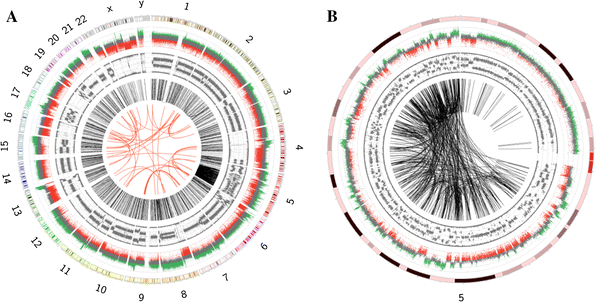
\includegraphics[width=\textwidth]{chapters/images/vcap/circosplots.png}
    \caption{\textbf{Circos plots showing structural and copy number variation across the whole genome (a) and chromosome 5 (b) of VCaP.} Each chromosome is represented
in the outer ring. The outer data ring corresponds to copy number variation, with regions of gain depicted in green and loss in red. The inner data ring
represents B-allele frequency. The intra and interchromosomal rearrangements are on the inside and depicted in black and red lines, respectively}\label{fig:vcap-circos}
\end{figure}


Out of the 573 SV breakpoints involving 5q, only four were interchromosomal with rearrangements to chromosomes 6 (three events) and 8 (\href{https://link.springer.com/article/10.1007/s00439-013-1308-1#SupplementaryMaterial}{Table S1}). Remarkably,
sequencing of the breakpoint junctions of these SV breakpoints revealed frequent insertions of novel sequences (186/573) (\href{https://link.springer.com/article/10.1007/s00439-013-1308-1#SupplementaryMaterial}{Table S2}). In the gene fusions
resulting from complex chromothripsis rearrangements in 5q, these insertions of up to 255 bp corresponded to fragments of chromosome 5 located within 7–53
Mb distance of the adjacent fusion partner. We rarely observe microhomology flanking the breakpoints in our set of gene fusions, and in a few cases,
we could detect repeats flanking in both sides of the breakpoint junction (\href{https://link.springer.com/article/10.1007/s00439-013-1308-1#SupplementaryMaterial}{Table S3}).


\begin{figure}
    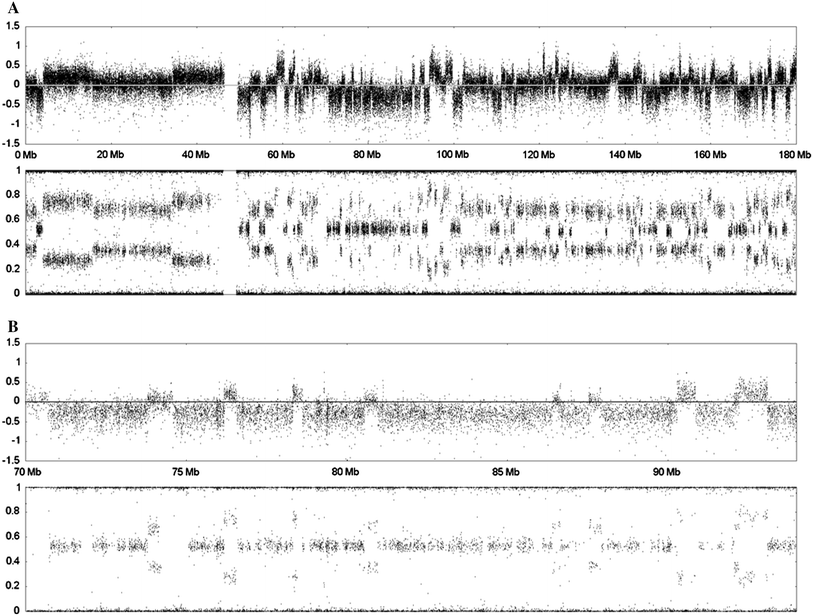
\includegraphics[width=\textwidth]{chapters/images/vcap/gnuplots.png}
    \caption{\textbf{Clustered rearrangements on chromosome 5q of VCaP.} Copy number across chromosome 5 oscillates between a copy number of 2, 3, and 4.
Copy number 2 corresponds to segments of SNP probes below the zero line, copy number 2 to segments of SNP probes in the zero line, and copy number
4 to segments of SNP probes above the zero line. The B-allele frequency plot is displayed below the copy number plot}\label{fig:vcap-gnuplot}
\end{figure}

Forty-three out of the 573 SV breakpoint events on 5q were in different genes at both sides. In 18 of the 43 events, the two different
genes were in the same orientation and potentially encoding a functional fusion protein (\hyperref[table:fusions]{Table~\ref*{table:fusions}}, \href{https://link.springer.com/article/10.1007/s00439-013-1308-1#SupplementaryMaterial}{Figure S2}). In order to validate
the 18 candidate gene fusions on DNA level and check whether the fusion transcripts encode an in-frame fusion protein, we performed
PCR on both DNA and cDNA level. We could validate 15 candidate gene fusions at the DNA level (\href{https://link.springer.com/article/10.1007/s00439-013-1308-1#SupplementaryMaterial}{Figure S3}), whereas only one-third were
detected on mRNA level suggesting downregulation of gene expression or instability of the fusion transcripts~\cite{stephens2011massive}.
Sequencing of the PDE4D-FAM172A breakpoint revealed that within this gene fusion a small fragment of PPP2R2B sequence (55 bp) is inserted
in-between the PDE4D and FAM172A genes. This explains the correct NGS identification of the PDE4D-PPP2R2B and PPP2R2B-FAM172A breakpoints,
 but the absence of a PCR product since the PPP2R2B primers were originally designed outside of the small insert. Conversely, the ADAMTS12-PXDNL
candidate gene fusion had a very low number of discordant mate pairs indicating the fusion event, and hence is most likely a sequencing artifact.
Chromothripsis, being a seemingly random process, results in highly altered chromosomes with numerous mutations and rearrangements. The formation
of gene fusions as a consequence of the chromothripsis event does not seem to be preferential over rearrangements occurring outside genes.
Moreover, we did not observe positive selection for in-frame fusion transcripts, since only one out of the five expressed fusion transcripts
resulted in a feasible fusion protein. The role of this fusion between NDUFAF2 and MAST4 remains to be determined (\href{https://link.springer.com/article/10.1007/s00439-013-1308-1#SupplementaryMaterial}{Figure S4, Table S4}). Using PCR,
we observed that all 15 fusions detected in VCaP were also present in the DuCaP cell line which is derived from a dura mater metastasis from the
same patient that gave rise to VCaP~\cite{lee2001establishment}, indicating that chromothripsis occurred in the cells that resulted in both VCaP and DuCaP
metastases (\href{https://link.springer.com/article/10.1007/s00439-013-1308-1#SupplementaryMaterial}{Figures S3 and S4}) (data not shown). The finding that both VCaP and DuCaP harbor the identical gene rearrangements identified in
chromosome 5 indicates that these were present in the precursor prostate adenocarcinoma lesion and not a cell line cultivation artifact.



\begin{table}[t!]
\begin{tabular}{llllllll}
\toprule
5' Donor & 3' Acceptor & Donor gene & Acceptor gene & Validated & Validated & In-frame & \# of Discordant  \\
gene & gene & Chr & Chr & cDNA & DNA & & mate pairs \\
\midrule
PDE4D & C5orf47 & 5 & 5 & Yes & Yes & No & 218 \\
CPLX2 & UBXD8 & 5 & 5 & No & Yes & No & 55 \\
EBF1 & FBXL17 & 5 & 5 & No & Yes & No & 74 \\
KCNN2 & EBF1 & 5 & 5 & No & Yes & Yes & 509 \\
RASGRF2 & RNF145 & 5 & 5 & No & Yes & No & 71 \\
JMY & DMGDH & 5 & 5 & Yes & Yes & No & 102 \\
TRIM40 & FBXO38 & 6 & 5 & No & Yes & No & 89 \\
LMAN2 & AP3S1 & 5 & 5 & Yes & Yes & No & 191 \\
EFNA5 & PCDHB7 & 5 & 5 & No & Yes & No & 11 \\
YTHDC2 & PPP2R2B & 5 & 5 & No & Yes & No & 8 \\
PDE8B & UIMC1 & 5 & 5 & No & Yes & No & 63 \\
ZFP62 & RGNEF & 5 & 5 & No & Yes & No & 225 \\
NDUFAF2 & MAST4 & 5 & 5 & Yes & Yes & Yes & 197 \\
ADAMTS12 & PXDNL & 8 & 5 & No & No & No & 3 \\
EBF1 & FEM1C & 5 & 5 & No & Yes & No & 11 \\
PDE4D & FAM172A & 5 & 5 & Yes & Yes & No & 119 \\
PDE4D & PPP2R2B & 5 & 5 & No & No* & No & 12 \\
PPP2R2B & FAM172A & 5 & 5 & No & No* & Yes & 7 \\
\toprule
\end{tabular}

\caption{\textbf{List of gene fusions involving chromosome 5 of VCaP.} The column \textit{Donor Gene Chr} refers to the chromosome number of the donor gene, and the column \textit{Acceptor Gene Chr} refers to the chromosome number of the 3' acceptor gene. The column \textit{\# of discordant mate pairs} displays the number of mate pair reads that are discordant in relation to the reference genome build 18 and concordant with the respective reported SV event (gene fusion). The \textit{*} corresponds to by-product events that do not result in a real gene fusion}\label{table:fusions}
\end{table}



In our whole genome study of VCaP cells, we also detected a fairly complex rearrangement involving the TMPRSS2 and ERG genes on chromosome 21q\@.
ehe TMPRSS2-ERG fusion in VCaP results from the assembly of the ERG and TMPRSS2 breakpoints with the insertion of two fragments of TMPRSS2 (\href{https://link.springer.com/article/10.1007/s00439-013-1308-1#SupplementaryMaterial}{Table S5}).
This did not disrupt the transcript and open reading frame of the final fusion product~\cite{mertz2007molecular}.

Recently, an association between TP53 mutations and chromothripsis has been observed for acute myeloid leukemia and pediatric
medulloblastoma~\cite{rausch2012genome}. In order to determine the status of TP53 in the VCaP cell line, we examined all the single
nucleotide variants (SNVs) detected by next generation sequencing in the TP53 gene (\href{https://link.springer.com/article/10.1007/s00439-013-1308-1#SupplementaryMaterial}{Table S6}). We observed two homozygous missense
SNVs present in the TP53 coding DNA sequence (CDS): c.742C>T and c.215C>G. The c.742C>T (p.R248 W) is a well-known frequently
observed mutation that fully inactivates TP53. The c.215C>G (p.R72P) is a natural occurring polymorphism in exon 4 of TP53.
As a result of the c.742C>T SNV, the VCaP cell line has no wild type functional p53, a key player in the maintenance of genomic
stability. In addition, we have also examined whether there were SNVs present in DNA repair genes previously shown to be altered
in prostate cancer~\cite{grasso2012mutational} (\href{https://link.springer.com/article/10.1007/s00439-013-1308-1#SupplementaryMaterial}{Table S7}). Interestingly, we found the genes ATM, MLH1, PRKDC, and ERCC5 to have missense
SNVs in their respective CDS\@. The only SNVs described to be mutational were present both in the ATM gene (COSMIC mutation ID number
21826 and 21827), but the functional relevance of these remains unknown~\cite{gumy2006atm}. An SNV present in the intron 7
acceptor splicing site of the XRCC4 gene (rs1805377) has shown to be significantly associated with increased prostate cancer risk~\cite{mandal2011polymorphisms}. The homozygous missense c.655A>G SNV present in the MLH1 gene (p.I219V) has been associated with increased
risk of colorectal cancer~\cite{campbell2009mismatch}. Deficiencies in the DNA mismatch repair system are commonly observed in colorectal
cancer and to a less extend in prostate cancer. The influence of the c.655A>G (p.I219V) missense SNV in the development of prostate
cancer remains undetermined.

Here, we report the structural variations detected in VCaP and show that the q arm of chromosome 5 has undergone chromothripsis.
Chromosome 5 appears to be frequently affected by chromothripsis with studies showing the same pattern in a renal cancer cell line~\cite{stephens2011massive} and a neuroblastoma patient~\cite{molenaar2012sequencing}. It remains undetermined, however, whether chromosome-specific
properties or the nonrandom radial localization of chromosomes in distinct territories play a role in the preferential target of certain
chromosomes by chromothripsis. Whether the catastrophic events on 5q in VCaP and the related cell line DuCaP have been playing and still
playing an important role in tumorigenesis remains to be determined.

The massive number of genomic breaks occurring in chromosome 5q hampers the formulation of a definitive model for the generation of chromothripsis.
The copy number variation and B-allele frequency of chromosome 5q in VCaP is a repetition of regions with n2 (AB), n3 (AAB), and n4 (AAAB) (\href{https://link.springer.com/article/10.1007/s00439-013-1308-1#SupplementaryMaterial}{Figure S1}).
Based on chromosome painting, VCaP is an overall near-triploid cell line with four copies of chromosome 5 that vary in size (~68–74(3n), XXYY)
(van Bokhoven et al. 2003). We hypothesize that this pattern is explained by two normal chromosome copies (n2 (AB)) and two copies of A with
chromothripsis (n4 (A*A*AB)), of which one of the two copies has undergone additional rearrangements resulting in n3 (A*AB). The sequence of
events that would lead to this pattern is a duplication of A and B (AABB) and subsequent loss of one B-allele (AAB). One of the A-alleles would
have undergone chromothripsis (A*AB) and duplication (A*A*AB). Additional rearrangements (deletions or even a second chromothripsis event) would
explain the observed 5q regions of n3 (A*AB) (\href{https://link.springer.com/article/10.1007/s00439-013-1308-1#SupplementaryMaterial}{Figure S5}). Our study has shown that research on genes located on and transcripts derived from
chromosome 5q need to take the chromothripsis into account. Besides, being a widely used model for research on AR, ERG, and CRPC, VCaP might
prove a highly relevant model for research on chromothripsis.

\section*{Acknowledgements}
This study was supported by the Complete Genomics Inc.\ grant (EMC GL 083111), the FP7 Marie Curie Initial Training Network PRO-NEST
(grant number 238278) and the CTMM (Center for Translational Molecular Medicine) Translational Research IT (TraIT).

%\includepdf[pages=1-5]{chapters/myarticles/VCaP.pdf}


\bibliographystyle{ieeetr}
\bibliography{references}

\begin{savequote}[75mm]
“I didn’t want to just know names of things. I remember really wanting to know how it all worked.”
\qauthor{Elizabeth Blackburn}
\end{savequote}

\chapter{Somatic Variant Detection}\label{chapter:virtualnormal}
\setcounter{figure}{-1}
\setcounter{table}{-1}
\setcounter{section}{-1}

\begin{figure}[t!]

\includegraphics[height=10em]{frontmatter/images/chapter-header-variants-tools.png}
\end{figure}
\setcounter{figure}{-1}
\setcounter{table}{-1}
\setcounter{section}{-1}


This chapter contains the following sub-chapters:

\begin{enumerate}[label=\ref{chapter:virtualnormal}.\arabic*]
\itemsep-0.5em
\item \textbf{CGtag:} Complete Genomics Toolkit and Annotation in a Cloud-based Galaxy
\item Discriminating somatic and germline mutations in tumor DNA samples without matching normals
\end{enumerate}

We integrated the Complete Genomics toolsuite into Galaxy and used it to analyse tumour samples without a matching normal.



  \setcounter{NAT@ctr}{-1}
\chapter*{}

\begin{figure}[t!]
\centering

\includegraphics[height=10em]{frontmatter/images/chapter-header-tools.png}
\end{figure}
\vspace{-4cm}

\phantomsection\addcontentsline{toc}{section}{The Informatics: CGtag}
\articletitle{CGtag: Complete Genomics Toolkit and\\Annotation in a Cloud-based Galaxy}\label{chapter:cgtag}
Saskia Hiltemann\textsuperscript{\ref{affil:emc},*},
Hailiang Mei\textsuperscript{\ref{affil:nbic}},
Mattias de Hollander\textsuperscript{\ref{affil:knaw}},
Ivo Palli\textsuperscript{\ref{affil:emc}},
Peter van der Spek\textsuperscript{\ref{affil:emc}},
Guido Jenster\textsuperscript{\ref{affil:emc-uro}},
Andrew Stubbs\textsuperscript{\ref{affil:knaw}}

\small
\begin{enumerate}
\itemsep-0.5em
\item Department of Bioinformatics, Erasmus Medical Centre, Rotterdam, The Netherlands.\label{affil:emc}
\item Netherlands Bioinformatics Center, NBIC, Nijmegen, The Netherlands\label{affil:nbic}
\item Department of Microbial Ecology, Netherlands Institute of Ecology, NIOO-KNAW, Wageningen, The Netherlands\label{affil:knaw}
\item Department of Urology, Erasmus Medical Centre, Rotterdam,  The Netherlands\label{affil:emc-uro}
\end{enumerate}
\normalsize

Published in: \emph{GigaScience}, 2014 Jan 24;3(1):1 \\
DOI: \url{https://doi.org/10.1186/2047-217X-3-1}

\section*{abstract}

\textbf{Background:} Complete Genomics provides an open-source suite of command-line tools for the analysis of their CG-formatted mapped sequencing files. Determination of; for example, the functional impact of detected variants, requires annotation with various databases that often require command-line and/or programming experience; thus, limiting their use to the average research scientist. We have therefore implemented this CG toolkit, together with a number of annotation, visualisation and file manipulation tools in Galaxy called CGtag (Complete Genomics Toolkit and Annotation in a Cloud-based Galaxy).


\textbf{Findings:} In order to provide research scientists with web-based, simple and accurate analytical and visualisation applications for the selection of candidate mutations from Complete Genomics data, we have implemented the open-source Complete Genomics tool set, CGATools, in Galaxy. In addition we implemented some of the most popular command-line annotation and visualisation tools to allow research scientists to select candidate pathological mutations (SNV, and indels). Furthermore, we have developed a cloud-based public Galaxy instance to host the CGtag toolkit and other associated modules.

\textbf{Conclusions:} CGtag provides a user-friendly interface to all research scientists wishing to select candidate variants from CG or other next-generation sequencing platforms’ data. By using a cloud-based infrastructure, we can also assure sufficient and on-demand computation and storage resources to handle the analysis tasks. The tools are freely available for use from an NBIC/CTMM-TraIT (The Netherlands Bioinformatics Center/Center for Translational Molecular Medicine) cloud-based Galaxy instance, or can be installed to a local (production) Galaxy via the NBIC Galaxy tool shed.

\textbf{Keywords:} Complete Genomics, Next Generation Sequencing, Genetic variation, Pathogenic gene selection.



\section*{Findings }

\subsection*{Background}

Complete Genomics (CG) supplies results for whole-genome next-generation sequencing (NGS) data mapped to a user-defined genome~\cite{ma} and additional open-source tools~\cite{url-cgatools} for further characterisation of the sequenced genomes. Whilst these tools are open-source and available for download and use on the command-line, they are not amenable for scientists to use from their desktop, and require scripting skills to link these tools together with other applications to successfully prioritise candidate pathogenic genes based on these NGS results. To address this issue, we implemented the Complete Genomics Analysis Toolkit (CGATools), including several functional annotation and visualisation tools in a cloud-enabled instance of Galaxy. Galaxy offers a web-based graphical user interface to command-line tools, and allows for the graphical construction of complex workflows; Galaxy will automatically keep track of the analysis history, and allows for easy sharing and publishing of data and/or workflows with other users~\cite{goecks2010galaxy, blankenberg2010galaxy2, giardine2005galaxy}. Furthermore, Galaxy is an extensible platform, nearly any software tool may be integrated into Galaxy, and there is an active community of users and developers ensuring the latest tools are made available for use in Galaxy through the Galaxy tool shed.

This implementation of the CGATools in a Galaxy environment simplifies the analysis of genomes via the Galaxy GUI and the cloud resource ensures that sufficient computing power is available for the analysis. The inherent functionality in Galaxy of CGtag enables the creation of customisable user-defined workflows by the scientist and not only by the bioinformatician.

For large datasets, transfer to Galaxy via SFTP is available and recommended, but is still limited by the upload speed of the user’s internet connection, and can be a bottleneck in the analysis of large datasets.


\subsection*{Variant Detection}

CGATools is an open-source project to provide tools for downstream analysis of Complete Genomics data, and may be downloaded from their repository~\cite{url-cgatools}. These tools must be run from the command-line and are therefore, not accessible to all users. To remedy this, Complete Genomics also provide Galaxy tool wrappers for many of the CGAtools, which can be downloaded from the Main Galaxy tool repository (tool shed)~\cite{url-toolshed}. However, these Galaxy tools still need to be installed on the users’ local (production) Galaxy instance before they can be utilised. We have now made these tools available on a public server~\cite{url-nbicgalaxy}, and have added Galaxy wrappers for those CGAtools that were not provided by Complete Genomics e.g. Junctions2Events, makeVCF (\hyperref[table:tools]{Table~\ref{table:tools}}). The use of the CGAtools in \hyperref[table:tools]{Table~\ref{table:tools}} have previously been outlined~\cite{nieminen}, using a combination of ListVariants and TestVariants or CallDiff to determine candidate pathogenic single nucleotide variants (SNVs), indels and subs in a selected genome as compared with on or more reference genomes or as part of a trio based genetic analysis~\cite{nieminen}. The VarFilter may be used to select those variants which have a high confidence based on the underlying sequence reads as specified as VQHIGH, and the SNPDiff tool can then be used to determine concordance of the NGS results with those of an orthogonal SNV detection platform such as an Affymetrix or Illumina SNP array. The JunctionDiff and Junction2Events tools are used to select fusion events and candidate fusion genes based on quality of the discordant reads used to detect the structural variation event~\cite{ifuse}.


\begin{table}[t!]
\small
\begin{tabular}{l|l|l}
\textbf{Function} & \textbf{CGATool}  & \textbf{Description} \\ \toprule
Variant detection & CGATools ListVariants & Lists the non-redundant set of small variations found in an \\
                  &                       & arbitrary number of genomes.\\
Variant detection & CGATools TestVariants & Determine which variants are found in which genomes given \\
                  &                       & the results of ListVariants.\\
Variant detection & CGATools CallDiff     & Compares two variant files to determine where and how the \\
                  &                       & genomes differ.\\
Variant detection & CGATools VarFilter    & Copies the input varfile or masterVar file, applying filters.\\
Variant detection & CGATools JunctionDiff & Reports difference between junction calls of CG junction files.\\
Variant detection & CGATools Junctions2Events & Groups and annotate related junctions.\\
Quality control   & CGATools SNPDiff      & Compares genotype calls to CG variant files.\\
File merge        & CGATools Join         & Merge two tab-delimited files based on equal field or overlapping \\
                  &                       & regions.\\
Sequence retrieval& CGATools DecodeCRR    & Retrieve sequences from a CRR file for a given range of a \\
                  &                       & chromosome.\\
File conversion   & CGATools mkVCF        & Converts CG variant and/or junction files to VCF.\\
File conversion   & CGATools generateMasterVar & Converts a varfile to a on-line-per-locus format.\\
File conversion   & CGATools fasta-2-crr  & Converts fasta sequences into a single reference crr file.\\
File conversion   & CGATools crr-2-fasta  & Converts crr file to fasta sequence.\\
File conversion   & TestVariants2VCF      & CG community tool. Converts output of the TestVariants tool \\
                  &                       & to VCF.\\
Annotation        & ANNOVAR               & Functional annotation of genetic variants from high-throughput \\
                  &                       & sequencing data.\\
Annotation        & MutationAssessor      & Functional impact of protein mutations.\\
Annotation        & Condel                & CONsensus DELeteriousness score of missense SNVs.\\
Visualisation     & CG Circos plots       & Create CG-style tumour, normal and somatic plots.\\
Visualisation     & Integrative plot      & Create circos plot from CG and SNParray data.\\
Visualisation     & Generic genomic data plotter & Plot any type of numerical genomic data using GNUplot.\\
File manipulation & Filter columns        & Filter tab-delimited files based on column contents.\\
File manipulation & Add/remove chr prefix & adds or removes chr prefix from chromosome column.\\
File manipulation & Column select         & Extract and/or rearrange columns in tab-delimited file.\\
File manipulation & Sort chromosomal position & Sort a tab-delimited file by chromosomal position.\\
File manipulation & Strip header          & Remove header from files.\\
File manipulation & File concatenation    & Concatenate 2 files (e.g.\ for restoring header).\\

\end{tabular}
\caption{Overview of CGTag tools available in NBIC/CTMM-TraIT Galaxy and the NBIC tool shed}\label{table:tools}
\end{table}
\normalsize


\subsection*{Functional Annotation Tools}

To provide users with enhanced filtering capabilities, we have integrated several command-line annotation tools in this NBIC/CTMM-TraIT Galaxy instance. ANNOVAR~\cite{annovar} is a command-line tool used to functionally annotate genetic variants. We provide a Galaxy tool wrapper for ANNOVAR\@. This tool will take a list of variants as input and provide gene and amino acid change annotation, SIFT scores, PolyPhen scores, LRT scores, MutationTaster scores, PhyloP conservation scores, GERP++ conservation scores, DGV variant annotation, dbSNP identifiers, 1000 Genomes Project allele frequencies, NHLBI-ESP 6500 exome project allele frequencies, and other information. We have implemented this tool to accept VCF (v4) files, Complete Genomics varfiles or CG-derived tab-separated files using the CG 0-based half-open coordinate system, or lastly, the standard ANNOVAR input format consisting of tab-separated lists of variants using the 1-based coordinate system. This tool will output the original file columns, followed by additional ANNOVAR columns. The ANNOVAR code itself is not included in the tool shed repository, but instructions on how to obtain a license and the subsequent manual installation of the tool are included in the readme of the Galaxy tool shed repository. We obtained permission to offer ANNOVAR on our public Galaxy server, so the tool can be previewed there. To supplement ANNOVAR, Condel (CONsensus DELeteriousness)~\cite{condel} has been included to calculate the deleterious score associated of missense SNVs and the impact of non-synonymous SNVs on protein function. Condel integrates the outputs of two tools: SIFT and Polyphen2, to calculate a weighted average of the scores (WAS) of these tools. Condel can optionally incorporate the output of a third tool, MutationAssessor, which is also included in this Galaxy instance. Mutation Assessor~\cite{mutass} is a web-based tool providing predictions of the functional impact of amino-acid substitutions in proteins, such as mutations discovered in cancer or missense polymorphisms. The MutationAssessor database is accessed through a REST API\@. In order not to overload the server, queries are limited to 3 per second, so when dealing with a long list of variants, some pre-filtering is recommended. The functional annotation provided by ANNOVAR, including the addition of multiple versions of dbSNP, the variants provided by Complete Genomics Public data from unrelated individuals only~\cite{url-cgftp} and 31 genomes from Huvariome~\cite{huvariome}, are available in this Galaxy instance. Huvariome provides the user with additional whole genome variant calls for those regions which are difficult to sequence and can retrieve the weighted allele frequency for each base in the human genome~\cite{huvariome}.



\subsection*{Visualisation Tools}

\begin{figure}[t!]
\centering
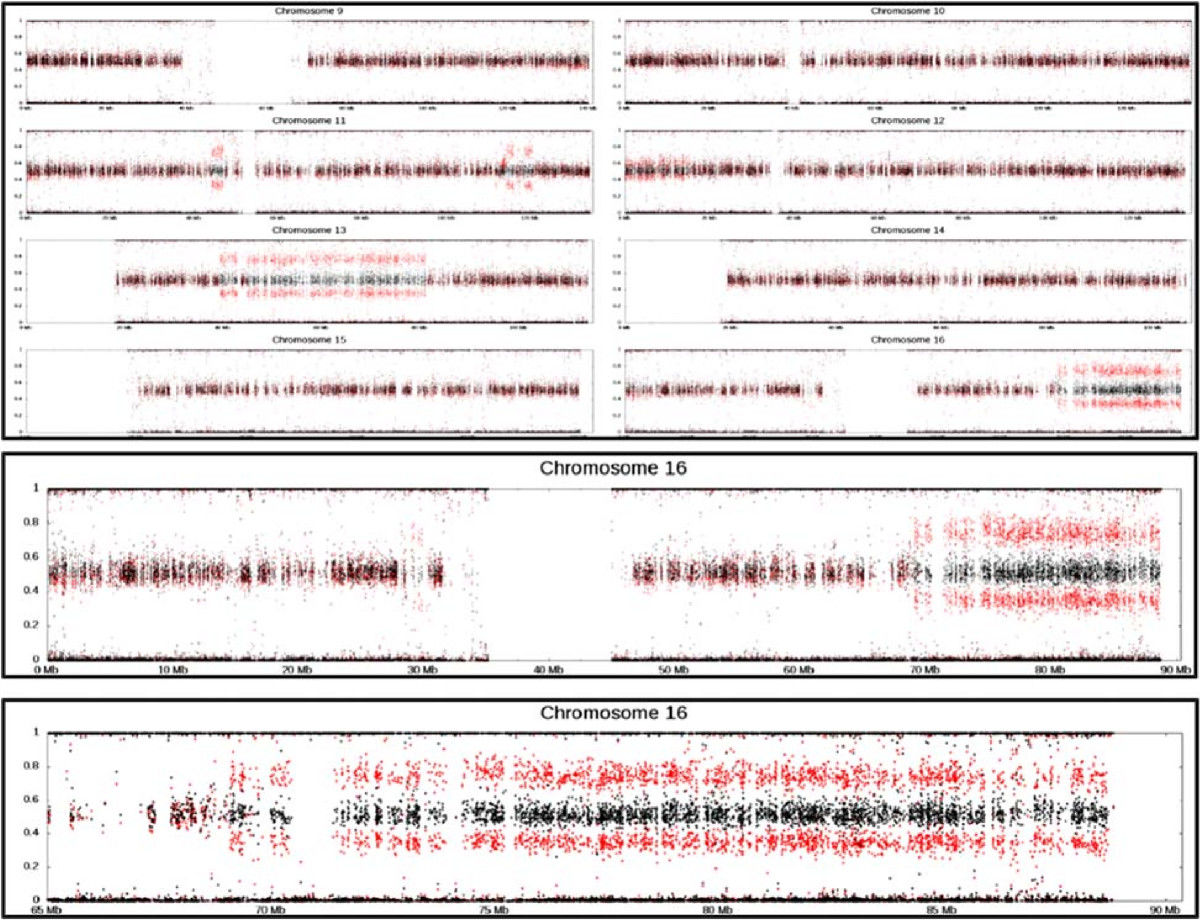
\includegraphics[scale=1.5]{chapters/images/cgtag/fig1-plotter.png}
\caption{\textbf{Generic Genomic data plotting tool.} Output from our generic genomic data plotter used to plot B-allele frequency from Illumina 1M SNParray data. Plot with two tracks; tumour (red) and normal (black). Output can be (top) a whole genome overview (shown here in part), or (middle) a single chromosome, or (bottom) a subregion of a chromosome defined by the user (here chr16, 60MB-end). Many parameters such as the colour and sizes of the data points may be adjusted by the user as required.}\label{fig:plotter}
\end{figure}


A generic genomic data plotter tool based on GNUplot is available, which takes as input, a tab-delimited file of format chr–start-end–value, and will output either a single chromosome plot, an overview of all chromosome plots in a single image, or a sub-region of a chromosome defined by the user. Additionally, the tool has the option of plotting input from a second file in the same image, which is useful for tumour-normal comparison (\hyperref[fig:plotter]{Figure~\ref{fig:plotter}}). B-allele frequency (BAF) is used to determine whether the structural variation junction is homo- or heterozygous. When the data is in the right format, the generic plotter tool can be used to visualise the BAF, and we have also implemented a plot tool to display allele frequencies directly from a CG masterVar file, again with the capability of displaying single-chromosome plots, all chromosomes in a single image, or custom defined regions (\hyperref[fig:plotter]{Figure~\ref{fig:plotter}}). The current Complete Genomics analysis pipeline (CGAP v2.5) delivers Circos~\cite{url-circos} visualisations with each genome that is sequenced and the code used to generate these images have been made freely available for download~\cite{url-cgcircos}. We have modified this code and implemented Galaxy tools to allow for the generation of these images for samples sequenced on earlier CG analysis pipelines (before v2.0), that utilise the junctions file, masterVar file, CNV details and CNV segments files to generate the standard CG Circos report.


To support fusion gene analysis we have created a custom Circos tool which uses CG files, CG junctions file and CG varfile for NGS, and the results from SNP arrays analysis, specifically the B-allele frequency (BAF) and copy number variation (CNV) files. The output is either a whole-genome plot, per-chromosome plots, a single image containing all the per-chromosome plots together, or a plot of a custom region defined by the user (e.g., a plot showing just chromosomes 3, 5, and X, or a plot showing a specific range within a single chromosome). Additionally the user can select an “impacted genes” track for the per-chromosome plots, which will print the names of the genes impacted by SV events along the outer edge of the image (\hyperref[fig:circos]{Figure~\ref{fig:circos}}). This custom Circos script is capable of using fusion gene detection results generated from the Illumina platform with the fusion genes detected by an application such as FusionMap~\cite{ge2011fusionmap}, and which are reported in custom FusionMap report format, a tab-delimited file similar to that delivered by Complete Genomics.


\begin{figure}[t!]
\centering
\includegraphics[scale=2]{chapters/images/cgtag/fig2-circos.png}
\caption{\textbf{Circos Integrative Plot Tool.} Circos plots for (left) whole genome, (middle) overview or all chromosomes in single images, and (right) for a single chromosome.  Each chromosome is represented in the outer ring and then from outer to inner rings represent copy number variation (with regions of gain depicted in green and loss in red), B-allele frequency, SNP density and the intra- and interchromosomal rearrangements are on the inside and depicted in black and red lines, respectively.  Impacted genes track (red gene symbols) are displayed outside the outer chromosome ring and only on the single chromosome plot.}\label{fig:circos}
\end{figure}


In addition to these tools within Galaxy, structural variation files processed using CGtag may be exported to our previously described fusion gene prioritisation tool, iFUSE~\cite{url-ifuse} to identify candidate fusion genes and display their representative DNA, RNA and protein sequence.


\subsection*{Auxiliary Tools}

Our suite of tools also includes several auxiliary tools supplied by CG but not available from the Galaxy tool shed which offer the user several file format conversion tools (\hyperref[table:tools]{Table~\ref{table:tools}}) that enable users to connect the output from the CGATools analysis to other analytical or annotation workflows by means of standard file formats (e.g., FASTA, VCF). In addition a number of file formatting tools are also included, such as removing of headers from files (required by some tools), adding removing of a chr prefix to a column of a file (i.e., chrX vs. X), concatenation of files, and extracting and rearranging of columns, to help facilitate the flow of data from one tool to the next.

\subsection*{CLOUD Implementation}

NBIC Galaxy is hosted at a high performance computing (HPC) cloud system operated by SURFsara~\cite{url-surfsara}. This HPC cloud consists of 19 fast servers with 608 CPUs and almost 5TB of memory. The NBIC Galaxy that operates in this HPC cloud is implemented using the Cloudman framework~\cite{afgan} and its adapted version supports the OpenNebula Cloud environment. The advantage of using the Cloudman framework to build NBIC Galaxy is mainly two-fold, firstly Cloudman provides a set of complete scripts to automatically install tools and datasets on a virtual machine image. The installed tools include the Galaxy system itself and all its dependencies. These dependencies include webserver (nginx), database (postgres), cluster job scheduler (SGE), and common NGS tools, such as bowtie, BWA, samtools, and so forth. The installed datasets include most of the common reference genomes (hg18, hg19, mm9, etc) and their tool-specific index files. Thus, the end product of running Cloudman installation script is a fully functional NBIC Galaxy system operating in the HPC Cloud.

The second contribution of Cloudman to our NBIC Galaxy system is its ability to set up a flexible virtual cluster and ability to provide auto-scaling support. The previous NBIC Galaxy was hosted on a dedicate physical server with rather limit resources (4 CPU, 32G memory). Due to this resource limitation, our NBIC Galaxy was never promoted to be a real data analysis server to handle the production level of NGS datasets. On the other hand, because of the sporadic nature of user access, the server was mostly on idle during its 2-year lifespan. Moving to Cloud resolved both issues. The current NBIC Galaxy operates on top of a virtual cluster. This virtual cluster contains one head node and a number of worker nodes. These nodes are all virtual machines that are built using the machine image generated by the Cloudman script. During minimal usage, the cluster will only contain one head node. Once a significant load occurs due to training courses or production level data analysis, the virtual cluster can automatically scale itself upwards. More worker nodes will be added dynamically to this virtual cluster to boost the capacity of NBIC Galaxy. Once the load decreases, the virtual cluster can scale down again to operate with only a limited number of nodes.

The use of shared resources does have drawback as well. We have experienced a more obvious I/O bottleneck in the cloud-based NBIC Galaxy compared to the previous system that ran in a physical machine. In the HPC Cloud, storage is provided through a network file system (NFS) instead of a local hard disk. When more concurrent Cloud users are using the Cloud resource, we observe the extra job time caused by I/O delays. However, we argue that this issue is far outweighed by the benefit of having a dynamic virtual cluster support to the NBIC Galaxy.


\section*{Availability and requirments}

\textbf{Project Name:} CGtag: Complete Genomics Toolkit and Annotation in a Cloud-based Galaxy\\
\textbf{Project home page:} http://galaxy-demo.trait-ctmm.cloudlet.sara.nl\\
\textbf{Operating system:} Linux (Galaxy and CGtag)\\
\textbf{Programming language:} Python (Galaxy and CGtag), R (CGtag), Bash (CGTag) \\
\textbf{Other requirements:} Circos~\cite{url-circos}, GNUplot~\cite{url-gnuplot}, Complete Genomics open source Toolset~\cite{url-cgatools}  and dependencies therein; see documentation for a comprehensive list of optional dependencies, based on workflow requirements.\\
\textbf{License:} GPL v3\\
\textbf{Any restrictions to use by non-academics:} ANNOVAR license must be obtained before it can be used\\
published page: http://galaxy.ctmm-trait.nl/u/saskia-hiltemann/p/cgtag \\
\textbf{Links to tool shed repositories:}\\
annovar: \url{http://toolshed.nbic.nl/view/saskia-hiltemann/annovar} \\
cgatools: \url{http://toolshed.nbic.nl/view/saskia-hiltemann/cgatools\_v17} \\
circos plotters: \url{http://toolshed.nbic.nl/view/saskia-hiltemann/cg\_circos\_plots} \\
condel: \url{http://toolshed.nbic.nl/view/saskia-hiltemann/condel} \\
file manipulation tools: \url{http://toolshed.nbic.nl/view/saskia-hiltemann/file\_manipulation} \\
generic genomic data plotter: \url{http://toolshed.nbic.nl/view/saskia-hiltemann/genomic\_data\_plotter} \\
mutation assessor: \url{http://toolshed.nbic.nl/view/saskia-hiltemann/mutation\_assessor}\\
NOTE:\ these tools can be installed to both Cloudman Galaxy instances or non-Cloudman Galaxy instances alike (via the tool shed or manually from the command line).

\section*{Availability and supporting data}

All tools described, as well as example data, are available from the NBIC/CTMM-TraIT Galaxy server (\url{http://galaxy.ctmm-trait.nl}) and the NBIC Galaxy tool shed (\url{http://toolshed.nbic.nl}).

\section*{Notes}

Saskia Hiltemann, Hailiang Mei, Mattias de Hollander, Ivo Palli, Peter van der Spek, Guido Jenster and Andrew Stubbs contributed equally to this work.

\section*{Abbreviations}

\textbf{BAF:} B-allele Frequency \\
\textbf{CG:} Complete Genomics \\
\textbf{CGATools:} Complete Genomics analysis tools \\
\textbf{CGtag:} Complete Genomics Toolkit and Annotation in a Cloud-based Galaxy\\
\textbf{NBIC:} The Netherlands Bioinformatics Center\\
\textbf{NFS:} Network File System \\
\textbf{SNV:} Single Nucleotide Variation\\
\textbf{SV:} Structural Variation\\


\section*{Declarations}

\subsection*{Acknowledgements}

This study was performed within the framework of CTMM, the Center for Translational Molecular Medicine. TraIT project (grant 05T-401).

This work was sponsored by the BiG Grid project for the use of the computing and storage facilities, with financial support from the Netherlandse Organisatie voor Wetenschappelijk Onderzoek (Netherlands Organisation for Scientific Research, NWO)

\subsection*{Note from the Editors}
This paper is part of the GigaScience Galaxy series. We will be hosting some of the computational resources of these papers on our GigaGalaxy server (http://galaxy.cbiit.cuhk.edu.hk).

\subsection*{Competing interests}

The authors declare that they have no competing interests.


\subsection*{Authors contributions}

H, GJ, HM and AS contributed to the design and coordination of CGtag and manuscript preparation. SH, MdH, IP and HM contributed to implementing CGtag.  SH, GJ, PvdS and AS contributed to testing of CGtag. MdH and HM implemented Galaxy Cloudman for the SURFsara/Big-grid HPC cloud. All authors read and approved the final manuscript.


\bibliographystyle{ieeetr}
\bibliography{references}

  \cleartorightpage
\setcounter{NAT@ctr}{-1}
\chapter*{}\label{chapter:vnmethod}

\begin{figure}[t!]
\centering
\includegraphics[height=10em]{frontmatter/images/chapter-header-variants.png}
\end{figure}
\vspace{-4cm}

\phantomsection\addcontentsline{toc}{section}{The Bio: Virtual Normal}
\articletitle{Discriminating somatic and germline mutations in tumor DNA samples without matching normals}\label{chapter:vnmethod-paper}

Saskia Hiltemann\textsuperscript{\ref{vn-affil:emc-bioinf}},
Guido Jenster\textsuperscript{\ref{vn-affil:emc-urology}},
Jan Trapman\textsuperscript{\ref{vn-affil:emc-pathology}},
Peter van der Spek\textsuperscript{\ref{vn-affil:emc-bioinf}},
Andrew Stubbs\textsuperscript{\ref{vn-affil:emc-bioinf}}

\small
\begin{enumerate}
\itemsep-0.5em
\item Department of Bioinformatics, Erasmus Medical Center, Rotterdam, The Netherlands. \label{vn-affil:emc-bioinf}
\item Department of Urology, Erasmus Medical Center, Rotterdam, The Netherlands \label{vn-affil:emc-urology}
\item Department of Pathology, Erasmus Medical Center, Rotterdam, The Netherlands. \label{vn-affil:emc-pathology}
\end{enumerate}

{\color{chaptergrey}{Published in:}} \emph{Genome Research}, 2015 Sep; 25(9): 1382–1390 \\
{\color{chaptergrey}{DOI:}} \hyperref[https://doi.org/10.1101/gr.183053.114]{10.1101/gr.183053.114}
% https://link.springer.com/article/10.1007/s10096-018-3220-z

\normalsize

\section*{Abstract}

Tumor analyses commonly employ a correction with a matched normal (MN), a sample from healthy tissue of the same individual, in order to distinguish germline mutations from somatic mutations. Since the majority of variants found in an individual are thought to be common within the population, we constructed a set of 931 samples from healthy, unrelated individuals, originating from two different sequencing platforms, to serve as a virtual normal (VN) in the absence of such an associated normal sample. Our approach removed (1) >96\% of the germline variants also removed by the MN sample and (2) a large number (2\%–8\%) of additional variants not corrected for by the associated normal. The combination of the VN with the MN improved the correction for polymorphisms significantly, with up to ∼30\% compared with MN and ∼15\% compared with VN only. We determined the number of unrelated genomes needed in order to correct at least as efficiently as the MN is about 200 for structural variations (SVs) and about 400 for single-nucleotide variants (SNVs) and indels. In addition, we propose that the removal of common variants with purely position-based methods is inaccurate and incurs additional false-positive somatic variants, and more sophisticated algorithms, which are capable of leveraging information about the area surrounding variants, are needed for optimal accuracy. Our VN correction method can be used to analyze any list of variants, regardless of sequencing platform of origin. This VN methodology is available for use on our public Galaxy server.

\section*{Introduction}

Analysis of 1092 human genomes performed by the 1000 Genomes Project reveals that an individual has approximately 4 million variations (on average, 3.7 million SNPs, 350,000 insertions and deletions [indels], and 750 large deletions) compared with the reference genome and that the vast majority of an individual's germline variations are polymorphic within the human population, with >95\% of all single-nucleotide variants (SNVs) and small indels in a given individual occurring at a frequency of ≥0.5\%~\cite{10002010map,10002012integrated}. Therefore, whenever a matched normal (MN) sample was unavailable (most commonly due to lack of funds or sample availability), researchers have typically relied on the public mutation databases and/or a set of in-house genomes for the filtering of germline variants from the full set of variants found in a tumor sample~\cite{yoon2009sensitive,kumar2011exome}. In recent years, these catalogs of human variation have grown exponentially, causing some researchers to question the necessity of sequencing a MN control for every tumor sample~\cite{kumar2011exome}.

In this study, we address the questions of whether current mutation databases are complete enough to correct for common and rare polymorphisms and of how well this filtering performs compared with the correction with a MN sample.

There are many public databases of human variation available. The Single Nucleotide Polymorphism Database (dbSNP) is a free public archive for genetic variation within and across different species~\cite{sherry2001dbsnp}. Its latest build (138) contains over 63 million polymorphisms found within the human population. The 1000 Genomes Project (1000G) database contains polymorphisms encountered in a set of 1092 genomes of healthy individuals~\cite{10002010map,10002012integrated}. The NHLBI Exome Variant Server (EVS) contains exonic variants from over 6500 genomes (\url{http://evs.gs.washington.edu/EVS}).

In an effort to improve the control-free correction method further, we constructed what we call a virtual normal (VN). This is a set of 931 samples from healthy, unrelated individuals, whole-genome sequenced to high depth, originating from two different sequencing platforms. Our VN consists of 433 public samples from Complete Genomics~\cite{drmanac2010human}, sequenced in the context of the 1000G, as well as 498 samples sequenced on Illumina HiSeq technology by the Genome of the Netherlands (GoNL) Consortium~\cite{boomsma2014genome,francioli2014whole}.

For copy-number analysis of sequencing data, tools exist that correct for normal contamination in unmatched tumor samples~\cite{boeva2010control}. The idea of using a set of genomes for correction of copy-number variants has also been described~\cite{yoon2009sensitive}. Apart from a correction based on GC content, this read-depth method also corrects for regions found to have an increased or decreased copy number across all five of their samples (from healthy individuals) and therefore likely a polymorphism within the population. We aim to assess the validity of such an approach and extend it by applying it to structural variation (SV), as well as SNV and indel analysis, in whole-genome-sequenced cancer samples. Additionally, we investigate the minimal size of such a VN necessary for adequate filtering and assess the influence of different ethnicities within the set.

Variants in mutation databases are usually represented only by their position relative to the reference genome and the variant allele, as well as possibly a quality metric. The advantage of using a VN is that we can also leverage information about the area surrounding a variant (e.g., nearby variants in the same sample) to optimize correction. There are often several different ways to describe the same variant, possibly involving (slightly) different chromosomal positions, which means that comparison methods that require an exact match of position and variant nucleotides may be suboptimal, leading to false-positive somatic variants. The algorithm we use with our VN correction is capable of detecting equivalences of differently described variants by taking into account the reference sequence surrounding a variant, as well as neighboring variants. This provides a valuable improvement over correction using variant databases, where this contextual information is lost.

\section*{Results}

We evaluate the performance of the different correction methods on four tumor-normal pairs from two different tumor types (breast and prostate cancer). All of the samples were sequenced by Complete Genomics. Two of the samples were also sequenced using Illumina technology. We evaluate the correction of SNVs and indels of up to ∼50 bp, as well as the larger SVs. For the breast cancer samples, additional validation data were available from the COSMIC database, and we used these confirmed variants to assess the performance of the three different correction methods (MN, mutation databases, VN).

We have made our VN correction method available as a tool for the Galaxy workflow platform~\cite{giardine2005galaxy,blankenberg2010galaxy2,goecks2010galaxy} as part of our tumor analysis in Galaxy (TAG) tool suite~\cite{hiltemann2014cgtag}.

\subsection*{MN vs. VN}

We use three correction methods in order to determine the set of tumor-specific (somatic) variants: a correction for germline variants using a MN sample, a correction for polymorphisms using the VN, and a correction for polymorphisms using public mutation databases (dbSNP, 1000G, and EVS). All variants remaining after application of all three correction methods represent the (consensus) set of true somatic variants. A false-positive variant of a method is any variant remaining after correction, which would have been removed had we employed all three correction methods.

\subsection*{Structural variations}

There are far fewer common SVs, than SNVs and indels, present in public databases. And the few sources of common SVs contain almost exclusively copy-number variants (large indels) and almost none of the more complex SVs such as inversions and translocations. This makes filtering of tumor variants when there is no MN sample very challenging. The Database of Genomic Variants (DGV)~\cite{macdonald2013database} is currently the largest SV database, with approximately 200,000 variants. However, >99\% of these variants are copy-number changes (gains or losses), and the database contains only a limited number of the more complex structural variant types such as inversions and (balanced) translocations, while these are thought to be common in the normal population~\cite{feuk2006structural,10002010map,10002012integrated,mills2011mapping}. We additionally filtered using BreakSeq database~\cite{lam2010nucleotide}, BreakDB~\cite{korbel2009pemer}, and the 1000G SVs~\cite{10002010map,10002012integrated}, which collectively contain another 32,000 structural variants.

We compared the SVs found in the tumor sample to those in the online databases and the VN\@. We consider two SVs a match if both sides of the event occur within a small distance of the sides of the other SV (200 bp when originating from the same platform, 500 bp when cross-platform).

In the Complete Genomics samples, the VN method removed most of the germline structural variants also removed by the associated normal (∼97\%) while also removing a further 6\%–8\% of common variants not corrected for by the associated normal.

For the Illumina samples, the VN method removed fewer SVs than the MN but was still a huge improvement over using only the database filter. The Illumina HCC1187 sample had 132,045 SVs identified in the tumor sample, of which 1464 were of high quality (QUAL ≥ 200). By use of the VN filter, we removed 961 polymorphic variants from this list (\hyperref[fig:svcomparison]{Fig.~\ref{fig:svcomparison}}). Increasing the distance parameter further (to 2000–5000 bp) resulted in the filtering of more SVs than the MN.

\begin{figure}[t!]
\centering
\includegraphics[width=\textwidth]{chapters/images/virtualnormal/Hiltemann_Figure1.png}
\caption{\textbf{Comparison of matched normal (MN) and virtual normal (VN) methods for structural variations (SVs).} Correction of high-confidence SVs from Complete Genomics (left) and Illumina (right), using the database filter (DB), MN, and VN\@. Light gray area indicates the golden set (combination of the three).}
\label{fig:svcomparison}
\end{figure}

Experimental validation data for the two public genomes HCC1187 and HCC2218 were obtained from the COSMIC database~\cite{forbes2010cosmic,bindal2011cosmic}. We determined the number of these confirmed somatic SVs detected in each sample and determined the number of detected SVs that survived our correction method (\hyperref[table:table1]{Table~\ref{table:table1}}). The CG samples had higher sensitivity (detected more of the validated SVs), but for every tumor sample, those variants that were detected by the platform and determined somatic after correction with the MN all survived correction with VN and DB.

\small
\begin{table}[t!]
\centering
\begin{tabular}{lllll}
          & Sample  & Detected & Somatic & Description of variants called somatic \\ \hline
Illumina  & HCC1187 & 71 of 98 & 53 & 53 of 71 matches survived MN correction; \\
          &         &          &    & all of these survived DB+ VN correction \\
Illumina  & HCC2218 & 54 of 64 & 10 & 10 of 54 matches survived MN correction;\\
          &         &          &    & all of these survived DB+ VN correction \\
CG        & HCC1187 & 91 of 98 & 91 & All survived MN correction; \\
          &         &          &    & all of these survived DB+ VN correction \\
CG        & HCC2218 & 55 of 64 & 55 & All survived MN correction; \\
          &         &          &    & all of these survived DB+ VN correction \\
\end{tabular}
\caption{Number of confirmed somatic SVs (as described in COSMIC database) detected in the tumor samples by CG and Illumina, and the number of these variants that are labeled soatic after corrections with our VN method}
\label{table:table1}
\end{table}
\normalsize

\subsection*{SNVs and indels}

For the analysis of SNVs and indels for both the MN method and the VN method, we additionally filter variants for their presence in dbSNP~\cite{sherry2001dbsnp}, the 1000G~\cite{10002010map,10002012integrated}, and the EVS (\url{http://evs.gs.washington.edu/EVS}) using the ANNOVAR tool~\cite{wang2010annovar}.

In annotating with the online databases, we require an exact match of position, as well as a match in variant allele between the cancer sample and the variant described in the database. For dbSNP, we used the set of nonflagged variants (flagged variants are those for which SNPs <1\% minor allele frequency [MAF; or unknown], mapping only once to reference assembly, or flagged as “clinically associated”).

The Illumina FastTrack Cancer Service (\url{http://www.illumina.com/services/whole-genome-sequencing-services/sequencing-service-providers-ign/sequencing-services.ilmn}) identified 15,499 somatic SNVs in the HCC1187 sample and 27,823 in HCC2218, after correction with the MN sample. We evaluate performance of our method by correcting the list of all variants found in the tumor sample using our VN set and comparing the remaining variants to those variants determined to be somatic by Illumina's tumor-normal sequencing service.

Two variants are considered a match when they share the same chromosomal position, as well as the same variant allele. Because variants can often be described in various different yet equivalent ways, we used a more advanced correction method for those comparisons involving CG data (the TestVariants tool from CG's tool suite). Detecting these equivalencies is very important for variant comparisons and is discussed in more detail in a later section.

Variants remaining after application of all three filters (MN, database filter, and VN) represent the golden set of true somatic variants (11,409 SNVs for HCC1187 and 20,560 for HCC2218). We determined the number of false-positive somatic variants identified by several filter combinations (\hyperref[fig:snvcomparison]{Fig.~\ref{fig:snvcomparison}}; \href{https://genome.cshlp.org/content/25/9/1382/suppl/DC1}{Supplemental Data S2}). High-confidence variants determined by the VN method are those variants not present in any of the VN samples, and the position may not be no-called in more than ∼50\% of the samples. This is similar to the MN correction, where typically only those variants are reported that were called reference in the normal sample; tumor variants at positions that are no-called in the normal are usually not reported as (high-confidence) somatic variants.

The VN approach has similar performance to a MN for SNVs and indels and even removes more variants than the associated normal in some cases (\hyperref[fig:snvcomparison]{Fig.~\ref{fig:snvcomparison}}). However, be aware that this does not mean it removes all of the same variants as the normal but rather it removes an equally large, but different set of variants. There are always highly personal germline variants that can only be removed by the MN, but similarly, there are also polymorphisms that are only removed by the VN and not the single MN sample.

\begin{figure}[t!]
\centering
\includegraphics[width=\textwidth]{chapters/images/virtualnormal/Hiltemann_Figure2.png}
\caption{\textbf{Number of false-positive SNVs and indels identified per filtering method for Illumina (left) and Complete Genomics (right).} True positives (green) are those variants remaining after application of all filters (for VN, we did not use the high-confidence criterion to determine the set of true positives). DB denotes an aggressive database filter. HighConf VN+DB denotes the list of high-confidence somatic variants as determined by the VN and database filters. MN + DB denotes the list of high-confidence somatic variants after correction with a MN combined with the database filter. }
\label{fig:snvcomparison}
\end{figure}

Significant improvement is made over the situation where no MN is available and only aggressive filtering with public databases is used. The advantage of using a VN method rather than relying solely on databases is greatest for indels, which are less abundant in the public databases than SNVs and are more difficult to annotate using a purely position-based method because they can often be called in various different but equivalent ways.

To ascertain the quality of the somatic variants identified by our method, we determined several metrics such as Ti/Tv ratio (\href{https://genome.cshlp.org/content/25/9/1382/suppl/DC1}{Supplemental Data S3}). We see that the Ti/Tv ratio decreases as more filtering is performed, which is expected for the tumor-specific mutations, as these are more random in nature. Breast cancer specifically has been shown to favor transversion variants~\cite{liu2002genetic}. Mutational spectra of the somatic variants determined by our method were also investigated (\href{https://genome.cshlp.org/content/25/9/1382/suppl/DC1}{Supplemental Data S3}) and are consistent with the literature~\cite{rubin2009mutation} in terms of mutation patterns.

Validation data were obtained from COSMIC for both samples. We used this list to determine the number of these validated variants that were detected in the tumor samples by each platform and to determine how many survived correction by our VN method (\hyperref[table:table2]{Table~\ref{table:table2}}). Over 94\% of the validated variants were detected in each tumor data set, and of the detected variants, only one variant in one of the samples was filtered out only by the VN, indicating a possible false-negative of our method. One confirmed somatic variant in the HCC1187 sample (both Illumina and CG) was present in the associated normals, the public databases, and the VN (17 samples), indicating a possible false positive in the COSMIC database. One of the confirmed variants in COSMIC for the HCC2218 sample appeared in our VN nine times, as well as in the dbSNP, the EVS, and 1000G, for both Illumina and CG, indicating another possible false positive in COSMIC\@. For each of the samples, five confirmed somatic variants were present in the dbSNP (NonFlagged) database. These variants were not present in the VN, the 1000G data, or the EVS and thus are likely disease-related variants that should have been flagged in dbSNP but were not.

\small
\begin{table}[t!]
\centering
\begin{tabular}{lllll}
          & Sample  & Detected   & Somatic & Description of variants called somatic \\ \hline
Illumina  & HCC1187 & 82 of 86   & 75      & Five filtered by dbSNP; one by VN only(1x); \\
          &         &            &         & 1 N + DB + VN(17x) \\
Illumina  & HCC2218 & 178 of 182 & 172     & Five filtred by dbSNP; one in DB (dbSNP + \\
          &         &            &         & 1kG + EVS) +VN(19x)\\
CG        & HCC1187 & 82 of 86   & 76      & Five filtered by dbSNP;\\
          &         &            &         & one N + DB + VN(17x); \\
CG        & HCC2218 & 173 of 182 & 167     & Five filtered by dbSNP; one in DB (dbSNP + \\
          &         &            &         & 1kG + EVS) + VN(9x) \\
\end{tabular}
\caption{Number of confirmed somatic variants (as described in COSMIC database) detected in the tumor samples by CG and Illumina, and the number of these variants that are labeled soatic after corrections with our VN method}
\label{table:table2}
\end{table}
\normalsize

\subsection*{Size of VN}

\subsubsection*{Structural variations}
We determined the number of VN samples required for filtering of common germline SVs for each sample (\hyperref[fig:vnsize]{Fig.~\ref{fig:vnsize}}). For the Complete Genomics samples, after using about 50 VN samples, the same numbers of SVs are filtered out as when using the MN\@. A plateau is reached after about 120 VN samples, and adding additional normal samples filters out only a small number of additional SVs. Correction with the VN did not remove as many variants as the MN for the Illumina sample, though it still provides significant improvement over filtering with databases alone. A plateau is also reached for the Illumina samples at around 300 VN samples. Increasing the distance threshold for when to consider two SVs a match to 2000 - 5000 bp did result in correction of the same number of SVs as the MN but is likely less accurate.

\begin{figure}[t!]
\centering
\includegraphics[width=\textwidth]{chapters/images/virtualnormal/Hiltemann_Figure3.png}
\caption{Number of structural variants filtered out after each additional VN sample for Complete Genomics (left) and Illumina samples (right). Blue denotes the HCC1187 sample; red, CG HCC2218. Dashed lines indicate the level reached by correction with the associated normal. }
\label{fig:vnsize}
\end{figure}

\subsubsection*{SNVs and indels}
We investigated how many VN samples are necessary for adequate filtering (\hyperref[fig:vnsize2]{Fig.~\ref{fig:vnsize2}}). We are able to attach a confidence measure to the remaining somatic variants by determining the number of VN samples that are no-called at the variants’ locus (e.g., a variant at a position that was fully called reference in all 931 normals is more likely to be a true somatic variant than a variant that was also not detected in any of the VN samples but no-called in all normals).


\begin{figure}[t!]
\centering
\includegraphics[width=\textwidth]{chapters/images/virtualnormal/Hiltemann_Figure4_fixed.jpg}
\caption{\textbf{Number of SNVs and indels removed after filtering with each additional VN sample.} Black dashed line indicates the number of variants labeled as somatic when using only a database filter; red dashed line, the number of variants after correction with MN and the public databases; and the green dashed line, the golden set variants, those remaining after application of all correction methods. The shaded area indicates the number of variants remaining after VN filtering, ranging from all variants (upper bound) to highest-confidence somatic variants (lower bound).}
\label{fig:vnsize2}
\end{figure}

The SNV and indel analysis results separated by variant type are presented in \href{https://genome.cshlp.org/content/25/9/1382/suppl/DC1}{Supplemental Data S8}. The advantage of the VN method over a database correction was greatest for indels, likely due the fact that these variants can more often be described in various different ways and at slightly different positions and therefore benefit more from the enhanced correction algorithm used in our method than the SNVs. For both SNVs and indels, the number of variants removed is comparable to the number removed by the MN and is significantly more than database corrections alone.

Analysis of SNVs revealed that for the CG samples, about 200 samples are needed to obtain the same performance as using the online databases alone, and any additional genomes added beyond that point will improve the filtering of common variants even further. The Illumina samples required a greater number of CG normals, about 300. For indel variants, the number of normal needed to surpass performance of the online databases alone is fewer than 100 for both platforms. Indel variants can more often be described in different but equivalent forms than SNVs, which means they benefit most from the enhanced comparison method used in our VN approach. The performance is better for Complete Genomics samples than for Illumina samples, but for both platforms, the performance is significantly improved by not relying solely on public mutation databases.

\subsection*{Prostate Cancer Samples}
ince HCC1187 and HCC2218 samples are both cell lines, we analyzed two prostate cancer patient samples, G110 and G316, to demonstrate that our method also works for patient data. The results are described in more detail in the \href{https://genome.cshlp.org/content/25/9/1382/suppl/DC1}{Supplemental Data S7}. These two samples were sequenced by Complete Genomics and use genome build hg18. Out of our 931 VN samples, 85 were also available on hg18, so for this analysis we used a smaller VN\@. Despite this reduced number of normals, our method could still correct as many variants as the MN, requiring around 60–100 normals genomes to do so (20–40 for SVs).


\subsection*{Influence of ethnicity}

The influence of ethnicity on the correction power was checked for 54 VN genomes from the Complete Genomics’ diversity panel. This panel contains individuals from five different populations across the world. We found that while there was a clear difference between genomes from different races, this difference was <10\%, and the set as a whole is capable of correcting as efficiently as a MN regardless of the background of the individual (\href{https://genome.cshlp.org/content/25/9/1382/suppl/DC1}{Supplemental Data S6}).

\subsection*{Improved correction method}

When comparing the variants found in a (tumor) sample to lists of known polymorphisms, the method most often used is to compare start and end coordinates of the two variants, as well as the observed sequence, and if these three values are identical, the variants are considered equal. However, this approach may be too naïve as there are often various different ways of describing the same variant, depending on the surrounding (reference) sequence and nearby variants.

Consider the following very simple example: Given a reference sequence of CAG and a variant sequence of CAAG, do we describe the variant as an A having been inserted after the C or before the G? Both descriptions are equally valid, but the position of the inserted nucleotide will differ by one. There is no real community consensus on how to resolve these kinds of canonicalization issues, though left alignment is by far the most commonly used. However, the HGVS recommendations urge \textit{“for all descriptions [to use] the most 3′ position possible”}, which would imply right alignment of variants on forward strand genes (\url{http://www.hgvs.org/mutnomen/recs-DNA.html}).

Another example, and one of the most frequently observed types of annotation difficulties in our data sets, are so-called block substitutions. Whenever two SNVs occur within a 3-bp window and are observed on the same reads, Complete Genomics will call a single 2- or 3-bp substitution, while Illumina will simply call two SNVs. Complete Genomics chooses this approach in order to retain the knowledge that these two variants were encountered on the same allele and possibly within the same codon, which is important for the determination of the impact of the variant on the protein. While the observed sequence for both platforms was the same, the descriptions differ, and naïve comparison methods will not be able to detect the equivalence of these variants.

We identified four main classes of equivalent, but differently described SNVs and indels in our data sets:

\begin{enumerate}
\item \textbf {Multivariants.} A series of nearby SNVs and indels may also be described as a single, larger substitution in order to retain the knowledge that they occurred on the same allele. The block substitutions are an example of this class (\hyperref[fig:variantannotation]{Fig.~\ref{fig:variantannotation}A}).

\item \textbf{Subvariants.} A variant is present in both samples, but in one of the samples, it was adjacent to another variant so in that sample the variant was part of a larger variant (\hyperref[fig:variantannotation]{Fig.~\ref{fig:variantannotation}B}).

\item \textbf{Canonicalization.} The same variant sequence is observed in both samples, but it can be described at a different position and possibly with a different observed variant sequence (\hyperref[fig:variantannotation]{Fig.~\ref{fig:variantannotation}C}).

\item \textbf{Annotation issues.} Different variant callers and different file formats will have differences in the way they describe variants; for example, when there are multiple variants at the same locus, the descriptions in the VCF format will be different than had the variants occurred alone, turning SNVs into multinucleotide variants and turning simple indels into complicated descriptors (\hyperref[fig:variantannotation]{Fig.~\ref{fig:variantannotation}D}). For example, in the Illumina VCF files, variants of the following pattern are frequently observed: TCA → TA,TC\@. This indicates that on one allele, the C nucleotide was deleted; on another, the A nucleotide. However, had only the deletion of A occurred, the variant would have been described as CA → C, and thus, the position of the variant would also have been shifted by one. Similarly, had only the deletion of C occurred, the description of the variant would have been TC → T, with an unchanged position field. Many tools converting VCF to a one-line-per-variant format simply split on the comma (TCA → TA and TCA → TC). While it is usually not difficult to reduce these variants to their canonical forms, many tools do not handle this issue correctly, and databases may not always ensure that only canonical forms are entered.
\end{enumerate}

\begin{figure}[t!]
\centering
\includegraphics[width=0.6\textwidth]{chapters/images/virtualnormal/Hiltemann_Figure5.png}
\caption{\textbf{Examples of equivalent, but differently annotated variants.} (A) When several nearby bases are changed, this can be described as one large substitution or as several smaller ones, even though the resulting sequence is the same. (B) Variant was present, but changes were described as part of a larger variant. (C) Canonicalization issues: Variants can often be described at various different positions, and variants originating from different sources may use different conventions, which must be taken into account during comparisons. (D) In the VCF format, overlapping variants can result in a different description of variants than had they occurred in isolation, a subtlety not always dealt with correctly in comparison algorithms. }
\label{fig:variantannotation}
\end{figure}

When comparing variants originating from the exact same sequencing and processing pipelines, these issues are minimal, but when comparing variants from different sources, they become more pronounced and must be dealt with in order to maximize the utility of variant databases. We encountered these problems many times when doing comparisons to COSMIC variants and describe several examples in more detail in \href{https://genome.cshlp.org/content/25/9/1382/suppl/DC1}{Supplemental Data S4}.

The comparison algorithm we use for our VN correction (CGATools) is capable of detecting most of these equivalences between SNVs and indels and therefore reduces the number of false-positive somatic variants identified.

The description of SVs is even less standardized, making comparisons of variants originating from different sources even more challenging. The differences in calling conventions for SVs are discussed in \href{https://genome.cshlp.org/content/25/9/1382/suppl/DC1}{Supplemental Data S4}.

\subsection*{Tumor analysis in Galaxy}

Galaxy is a free and open-source web-based analysis platform for data intensive biomedical research~\cite{giardine2005galaxy,blankenberg2010galaxy2,goecks2010galaxy}. Our VN filtering method is available as a tool for the Galaxy platform as part of our TAG tool suite. The tool can be installed to a local Galaxy instance via the DTL (Dutch Techcenter for Life Sciences) tool shed (\url{http://toolshed.dtls.nl}). Additional normal samples can easily be added to the VN set in this tool. Further installation and usage instructions can be found within the tool's tool shed repository. The tools have been installed on our demo galaxy example (\url{http://galaxy-demo.ctmm-trait.nl/u/saskia-hiltemann/p/virtual-normal-analysis})~\cite{hiltemann2014cgtag}; however, due to limited resources, we have had to impose disk and job quotas and recommend installing the tool onto a local (production) Galaxy server for optimal performance. Information about installing and maintaining a Galaxy server is available from the Galaxy wiki (\url{http://galaxyproject.org}).

\section*{Discussion}

We have developed a method for the filtering of tumor variants in the absence of a MN sample. To this end, we have constructed a VN consisting of a set of 931 whole genomes from healthy, unrelated individuals (433 sequenced by Complete Genomics, 498 by Illumina). We evaluated our method on four tumor-normal pairs of two different cancer types, from two different sequencing platforms (CG and Illumina), for both SVs and SNVs and indels. We found that such a VN can correct as many variants as a MN (and in many cases even more), allowing it to possibly serve as a substitute for a MN sample in a research context or provide a valuable addition to the MN in a more clinical setting where highest accuracy is required. It offers a huge improvement over the use of public databases alone, for example, in situations where no normal tissue is available.

Germline variations detected in these tumors after correction with associated normal are in the range of 80\%–85\% for SVs and 90\%–96\% for SNVs and small indels and substitutions. Our VN method is able to filter out most of these germline variants (96\%–99\%) and removes a large number of additional common variants not detected by the associated normal sample. The consensus set of variants—those remaining after correction with associated normal, VN, and public mutation databases—represents the set of true somatic variants. Our method identifies ∼10\%–30\% false-positive SVs and 20\%–30\% false-positive SNVs and indels, while the tumor-normal method has ∼20\%–50\% and 40\%–45\% false positives for SVs and SNVs and indels, respectively. This suggests that a VN could act as a substitute for an associated normal when the latter is unavailable, and even outperforms the standard MN correction in terms of false-positive rate in some samples.

The reason for the observation that correction using a VN collection can outperform the MN could be that the sequencing of a single MN sample will not call all germline variants. At the moment with an approximately 100× coverage single-sample analysis by Complete Genomics, ∼2.5\% of bases (∼70,000,000 bases) are not called. If these noncalls are random, a collection of samples will always outperform the correction using a single control. Therefore, we conclude that at the current coverage of 100× or less, a single normal matched control for correction of germline variants should be supplemented with (or even replaced by) a series of at least 200 control genomes in order to deliver optimal results.

We also investigated the optimal size of the VN set and determined that approximately 200–400 genomes are required in order to correct at least as efficiently as the MN sample for SNVs (fewer were required for CG-sequenced samples, as our VN also consisted of CG-sequenced samples). For SVs, 10–40 genomes were required for the CG samples, and for the Illumina samples, our 433 VN samples corrected fewer variants than the associated normal, largely owing to the fact that the description of breakpoints differs so greatly between the two platforms; were we to construct a VN of Illumina-sequenced samples, results would likely vastly improve.

Furthermore, we argue that using a purely position-based annotation incurs additional false positives, should be replaced by an algorithm capable of detecting the equivalence of variants called in different forms, and has knowledge of the reference genome and other nearby variants. When comparing variants obtained from the same sequencing platform and called using the same algorithm, a purely position-based method could suffice, but public databases often contain variants from various sources and are called using various different (versions of) algorithms; in order to utilize the full power of these databases, algorithms need to be able to detect equivalence of variants called in different forms and/or at different locations.

Some caveats to this approach exist: a VN approach cannot correct for those germline variants that are highly personal. Therefore, additional care must be taken when submitting variants to public databases to ensure the anonymity of the patient. In addition, the possibility exists that by foregoing the sequencing of a normal sample, rare germline variants may be mistakenly labeled as somatic, which may lead to rare heritable mutations being overlooked. Additional validation of the somatic status of the variants may be desirable in these cases, either by work in the laboratory or by considering larger groups of patients.

We are able to attach a confidence measure to the somatic variants as determined by our VN method by considering the number of VN samples that are no-called at the variants’ loci. A somatic variant at a position that was fully called reference in all 931 normals is more likely to be a true somatic variant than a variant that was also not detected in any of the VN samples but was no-called in all normal samples (i.e., evidence of absence vs.\ absence of evidence). Currently, this could only be done for the VN samples sequenced by CG, as the Illumina data does not provide the necessary information about no-called and half-called loci.

Our VN correction with the 931 samples can be run on any VCF file or list of variants, regardless of the sequencing platform of origin, and is available as a Galaxy tool from the DTLS tool shed (\url{http://toolshed.dtls.nl/repos/saskia-hiltemann/virtual\_normal\_preprocessing}) and is installed on our public demonstration Galaxy server (\url{http://galaxy-demo.ctmm-trait.nl}).

\section*{Methods}

\subsection*{Illumina vs. Complete Genomics}

For this study we analyzed two breast cancer cell line samples, HCC1187 and HCC2218, which have been whole-genome-sequenced by both Complete Genomics and Illumina and are publicly available for download (\url{ftp://ftp2.completegenomics.com/Cancer\_pairs/} and \url{https://basespace.illumina.com/datacentral}).

Comparisons between the Illumina and Complete Genomics platforms have been previously described~\cite{lam2012performance}. We compared the variants identified by each of the platforms for our samples and found that >96\% of the SNVs and >70\% of the indels identified by Complete Genomics were also present in the Illumina samples (\href{https://genome.cshlp.org/content/25/9/1382/suppl/DC1}{Supplemental Data S1}).

The description of SVs differs greatly between the two platforms, making comparison a challenging task. Our algorithm found an overlap of ∼40\%–45\% (\href{https://genome.cshlp.org/content/25/9/1382/suppl/DC1}{Supplemental Table S1.3}). The calling differences and comparison pitfalls are discussed in a later section.

\subsection*{Complete Genomics samples}

The HCC1187 breast cancer (primary ductal carcinoma) sample was TNM stage IIA, grade 3. For HCC1187 BL, the normal sample was derived from peripheral blood and immortalized with EBV transformation. ATCC numbers were as follows: tumor, CRL-2322; normal, CRL-2323. CG Software version used was 2.0.2.15.

The HCC2218 breast cancer (primary ductal carcinoma) sample was TNM stage IIIA, grade 3. For NA12880, the normal sample was derived from peripheral blood and immortalized with EBV transformation. ATCC numbers were as follows: tumor, CRL-2343; normal, CRL-2363. CG Software version used was 2.0.2.15.

Samples have been sequenced to an average genome-wide coverage of 123× for three of the samples and 92× for the NA12880 sample. The HCC1187 and HCC2218 samples were downloaded from Complete Genomics (\url{ftp://ftp2.completegenomics.com/Cancer\_pairs/}).

The prostate cancer sample G110 is derived from a radical prostatectomy. The tumor section from which DNA was isolated had a Gleason score of 3 + 3 and contained 80\% epithelial tissue, of which 90\% was cancer. The MN DNA was isolated from peripheral blood. The G110 and MN samples were sequenced by Complete Genomics to an average genome-wide coverage of 94× and 109×, respectively. The software version used was 2.0.2.24.

The prostate cancer sample G316 is derived from a transurethral resection of the prostate (TURP). The tumor section from which DNA was isolated had a Gleason score of 4 + 3 and contained only epithelial tissue, of which 100\% was cancer. The MN DNA was isolated from peripheral blood. The G316 and MN samples were sequenced by Complete Genomics to an average genome-wide coverage of 112× and 113×, respectively. The software version used was 2.0.2.24.
VN samples

The 433 normal samples were sequenced by Complete Genomics in the context of the 1000G and are accessible for download from the EBI and NCBI ftp servers at \url{ftp://ftp.1000genomes.ebi.ac.uk/vol1/ftp/} or \url{ftp://ftp-trace.ncbi.nih.gov/1000genomes/ftp/}.

For the hg18 prostate cancer samples, our VN set contained 66 normals, consisting of (1) the Complete Genomics diversity panel (46 genomes), (2) the four unrelated individuals from the CG pedigree, (3) the parents in the two CG trios (YRI and PUR), and (4) 12 in-house samples of healthy, unrelated individuals. This amounts to a total of 66 genomes. For the SNV and indel analysis, an additional 19 in-house samples were available, bringing the total up to 85. The Complete Genomics public samples may be downloaded from \url{ftp://ftp2.completegenomics.com/}. A list of all variants found in our in-house VN samples is available as a (public) shared data set from our demonstration Galaxy server (\url{http://galaxy-demo.ctmm-trait.nl}) and in the \href{https://genome.cshlp.org/content/25/9/1382/suppl/DC1}{Supplemental Materials}.

For the Illumina normals, sample-level data were obtained from the GoNL Consortium (\url{http://www.nlgenome.nl}) to perform this analysis. Our tool will only output summary counts for these data as the individual-level data are restricted.
Comparison to COSMIC validated variants

The validated variants obtained from COSMIC used hg19 coordinates, while our in-house samples were sequenced on hg18. The public CG samples were sequenced on both hg18 and hg19, so for this comparison, we used a VN consisting of just the 54 public hg19 genomes because a lift-over of genomic coordinates is suboptimal.

\subsection*{SV analysis}

We used CGATools JunctionDiff version 1.6 with default parameter settings for both the tumor-normal filtering and the tumor-VN filtering of the Complete Genomics samples. This means we considered two junctions to be the same when both the left sides and the right sides of the two junctions are on the same strand and fall within 200 bp of each other. For comparisons involving Illumina SVs, we created a custom script labelling two SVs as similar if they fall within a short distance of each other (for both sides of the event). We used a distance of 500 bp if the events came from the same platform, 1000 if they came from different technologies.

The CGATools source code and binaries are freely available for download at \url{http://cgatools.sourceforge.net}.

HCC1187 validation data in COSMIC are available at \url{http://cancer.sanger.ac.uk/cosmic/sample/overview?id=749711}. Data describe breast tissue, and the carcinoma is ductal. The number of genes examined is 4675; simple mutations, 29; gene fusions, 12; and structural variants, 94.

HCC2218 validation data in COSMIC are available at \url{http://cancer.sanger.ac.uk/cosmic/sample/overview?id=749716}. Data describe breast tissue, and the carcinoma is ductal. The number of genes examined is 4670; simple mutations, 76; gene fusions, 0; and structural variants, 62.

\subsection*{SNV and indel analysis}

We used the Complete Genomics CGATool ListVariants and TestVariants (version 1.6) for our SNV and indel analysis when comparisons involved CG data. When comparing Illumina tumors to Illumina VNs, we used vcftools (\url{http://vcftools.sourceforge.net}) and vcflib (\url{http://github.com/ekg/vcflib}), which compares positions as well as observed variant sequence when determining a match.

We used ANNOVAR (release date 2013 Feb 11) for annotation with the public variant databases. In annotating with the online databases, we require an exact match of position, as well as a match in variant allele between the cancer sample and the variant described in the database. For dbSNP, we used the set of nonflagged variants (flagged variants are those for which SNPs <1\% MAF (or unknown), mapping only once to reference assembly, or flagged as “clinically associated”).

HCC1187 validation data are available at \url{http://cancer.sanger.ac.uk/cosmic/sample/overview?id=1235080}. Data describe breast tissue, and the carcinoma is ductal. The number of genes examined is 12,196; simple mutations, 55; gene fusions, 0; and structural variants, 0.

HCC2218 validation data are available at \url{http://cancer.sanger.ac.uk/cosmic/sample/overview?id=1235085}. Data describe breast tissue, and the carcinoma is ductal. The number of genes examined is 12,196; simple mutations, 107; gene fusions, 0; and structural variants, 0.

dbSNP annotations are from the Database of Single Nucleotide Polymorphisms (dbSNP), National Center for Biotechnology Information, National Library of Medicine (dbSNP Build ID: all builds up to 38), and are available at \url{http://www.ncbi.nlm.nih.gov/SNP/}.

\subsection*{Data access}

WGS variation data from this study are available at the European Nucleotide Archive (ENA; http://www.ebi.ac.uk/ena), accession number PRJEB9673. The list of variants present in our 31 in-house normal samples can be found in the \href{https://genome.cshlp.org/content/25/9/1382/suppl/DC1}{Supplemental Material}.

\subsection*{Acknowledgments}

We thank Rick Tearle and Steve Lincoln from Complete Genomics, whose valuable discussions on Complete Genomics analysis methods supported our study. This study was performed within the framework of the Center for Translational Molecular Medicine (CTMM), TraIT project (grant 05T-401). This study makes use of data generated by the Genome of the Netherlands Project. A full list of the investigators is available from www.nlgenome.nl. Funding for the project was provided by the Netherlands Organization for Scientific Research under award no. 184021007, dated July 9, 2009, and made available as a Rainbow Project of the Biobanking and Biomolecular Research Infrastructure Netherlands (BBMRI-NL). The sequencing was carried out in collaboration with the Beijing Institute for Genomics (BGI). This work was sponsored by the BiG Grid project for the use of the computing and storage facilities, with financial support from the Nederlandse Organisatie voor Wetenschappelijk Onderzoek (Netherlands Organization for Scientific Research, NWO).

\footnotesize
\bibliographystyle{ieeetr}
\bibliography{references}
\normalsize

\cleartorightpage
\begin{savequote}[75mm]
“The more clearly we can focus our attention on the wonders and realities of the universe about us, the less taste we shall have for destruction.”
\qauthor{Rachel Carson}
\end{savequote}

\chapter{Microbiota Profiling}\label{chapter:microbiota}
\setcounter{figure}{-1}
\setcounter{table}{-1}
\setcounter{section}{-1}

\begin{figure}[t!]
\includegraphics[height=10em]{frontmatter/images/chapter-header-microbiota-tools.png}
\end{figure}
\setcounter{figure}{-1}
\setcounter{table}{-1}
\setcounter{section}{-1}

With sequencing costs steadily decreasing, 16S sequencing has become a viable alternative to culture-based methods in routine clinical diagnostics. For any clinical application, extensive validation is required. To pilot the utility of 16S profiling in a clinical setting, we first integrated the full mothur toolsuite into Galaxy (GmT), and subsequently used this toolsuite to create a set of workflows for clinical experimental designs in collaboration with Streeklab Haarlem (MYcrobiota).

This chapter contains the following sub-chapters:

\begin{enumerate}[label=\ref{chapter:microbiota}.\arabic*]
\itemsep-0.5em
\setcounter{enumi}{-1}
\item \textbf{Galaxy mothur Toolset (GmT):} a user-friendly application for 16S rRNA gene sequencing analysis using mothur
\item \textbf{MYcrobiota:} Development and evaluation of a culture-free microbiota profiling platform for clinical diagnostics
\end{enumerate}



  \cleartorightpage
\setcounter{NAT@ctr}{-1}
\chapter*{}\label{chapter:gmt}

\begin{figure}[t!]
\centering
\includegraphics[height=10em]{frontmatter/images/chapter-header-tools.png}
\end{figure}
\vspace{-4cm}

\phantomsection\addcontentsline{toc}{section}{The Informatics: GmT}
\articletitle{Galaxy mothur Toolset (GmT): a user-
friendly application for 16S rRNA gene sequencing analysis using mothur.}
Saskia Hiltemann\textsuperscript{\ref{gmt-affil:emc-bioinf},*},
Stefan Boers\textsuperscript{\ref{gmt-affil:emc-microbiology},*},
Peter van der Spek \textsuperscript{\ref{gmt-affil:emc-bioinf}},
Ruud Jansen\textsuperscript{\ref{gmt-affil:streeklabhaarlem}},
John Hays\textsuperscript{\ref{gmt-affil:emc-microbiology}},
Andrew Stubbs\textsuperscript{\ref{gmt-affil:emc-bioinf}}

\small
\begin{enumerate}
\itemsep-0.5em
\item Department of Bioinformatics, Erasmus Medical Center, Rotterdam, The Netherlands.\label{gmt-affil:emc-bioinf}
\item Department of Medical Microbiology and Infectious Diseases, Erasmus Medical Centre, Rotterdam, The Netherlands\label{gmt-affil:emc-microbiology}
\item Department of Molecular Biology, Regional Laboratory of Public Health Kennemerland, Haarlem, The Netherlands.\label{gmt-affil:streeklabhaarlem}
\end{enumerate}

{\color{chaptergrey}{Published in:}} \emph{GigaScience}, 2019 Feb 1;8(2):giy166 \\
{\color{chaptergrey}{DOI:}} \url{https://doi.org/10.1093/gigascience/giy166} \\
{\color{chaptergrey}{*:}} Saskia D. Hiltemann and Stefan A. Boers contributed equally to this work.


\section*{Abstract}
\textbf{Background} The determination of microbial communities using the mothur tool suite (\url{https://www.mothur.org}) is well established. However, mothur requires bioinformatics-based proficiency in order to perform calculations via the command line. Galaxy is a project dedicated to providing a user-friendly web interface for such command line tools (\url{https://galaxyproject.org/}).

\textbf{Results:} We have integrated the full set of 125+ mothur tools into Galaxy as the Galaxy mothur Toolset (GmT) and provided a set of workflows to perform end-to-end 16S rRNA gene analyses and integrate with third-party visualization and reporting tools.  We demonstrate the utility of GmT by analysing the mothur MiSeq standard operating procedure (SOP) data set (\url{https://www.mothur.org/wiki/MiSeq\_SOP}).

\textbf{Conclusions:} GmT is available from the Galaxy Tool Shed, and a workflow definition file and full Galaxy training manual for the mothur SOP have been created. A Docker image with a fully configured GmT Galaxy is also available

\textbf{Keywords:} Microbial classification; 16S rRNA gene sequence analysis; mothur

\section*{Findings}

\subsection*{Introduction}
 rRNA gene profiling analysis can be achieved using an extensive array of sophisticated software including mothur~\cite{schloss2009introducing}, QIIME~\cite{caporaso2010qiime}, MG-RAST~\cite{glass2010using}, and many more~\cite{oulas2015metagenomics}. Whilst some of these applications have a graphical user interface (GUI) to provide access to these technologies for the research scientist, their use remains complex for non-bioinformaticians. In this respect, the Galaxy project~\cite{afgan2016galaxy} was developed in order to simplify the use of complex command line software tools. Galaxy offers extensive support for both 16S rRNA gene-based and broader metagenomic analyses, with over 100 tools in the metagenomics section of the Galaxy tool shed, including QIIME~\cite{caporaso2010qiime}, KRONA~\cite{ondov2011interactive}, PyNAST~\cite{caporaso2009pynast}, PICRUSt~\cite{langille2013predictive}, Kraken~\cite{wood2014kraken}, MetaPhlAn2~\cite{truong2015metaphlan2}, HUMAnN2~\cite{abubucker2012metabolic}, PrinSEQ~\cite{schmieder2011quality}, Nonpareil~\cite{rodriguez2013nonpareil}, Vegan~\cite{dixon2003vegan}, and many more.

Mothur is an open-source application that was designed as a single piece of software capable of analysing and comparing microbial communities from 16S rRNA gene data derived from next-generation sequencing (NGS). The creators of mothur did not only provide an extensive set of tools, but also a collection of standard operating procedures (SOPs) that detail the recommended analytical protocol for different types of input data.

The latest version of mothur consists of over 125 components, lending it great flexibility, but at the same time, great complexity. To address this challenge, we have integrated the full set of 125+ mothur components into Galaxy that are collectively called the `Galaxy mothur Toolset (GmT)`. To simplify usage of GmT we provide the full workflow definition files, usage of which shields the end-user from the full complexities of the analysis. By simultaneously providing access to all the individual components present in mothur as separate tools, expert users and bioinformaticians retain the ability to utilize the full flexibility of mothur by creating custom workflows or by modifying or extending our workflows to fit their use-case.

GmT also leverages Galaxy's collections framework to enable easy analysis of large numbers (many thousands) of samples at once. Many mothur components support parallel computing, and the Galaxy tools will utilize the maximum amount of processing power alloted to them by the instance administrator. As part of GmT, datatypes were also contributed to the Galaxy core codebase to facilitate the handling of mothur-specific datatypes within Galaxy. Furthermore, a Galaxy data manager was also created for the automatic installation and configuration of reference datasets utilized by the mothur tool suite. And lastly, a Galaxy Interactive environment (GIE)~\cite{helena2015galaxy} for Phinch~\cite{bik2014phinch} was also developed~\cite{phinchGIE}.

GmT includes tools to produce standard file formats, such as the BIOM format~\cite{biom-format} to facilitate interoperability with these downstream analysis components. Where no clear file standards exists, GmT provides custom tools for conversion of mothur datatypes to other tools (e.g.\ the taxonomy-2-krona tool). This allows for integration with third party tools such as PICRUSt for prediction of functional content, or visualisation tools such as Phinch, KRONA, and certain QIIME components. The mothur tools also natively support incorporation of some 3rd party analysis tools, such as UCHIME and ChimeraSlayer for chimera detection or VSEARCH for clustering, which are also available in GmT.

The Galaxy Training Network (GTN) is a network of people and groups that present Galaxy and Galaxy-based training around the world. The GTN has created a central repository~\cite{gtn-repo} for Galaxy training materials. In order to further facilitate the use of GmT to end-users, we have contributed training materials to the GTN that illustrate how to run mothur's MiSeq SOP within Galaxy~\cite{gmt-training}. This work has also been incorporated in a larger-scale framework to easily and quickly explore microbiota data in a reproducible and transparent environment~\cite{batut2017asaim}.

\subsection*{Purpose of this work}
The work performed and described in this technical note has four objectives. First to provide end-users and bioinformaticians with easy access to all the mothur tools as the GmT. Second is to provide open-access online training material to demonstrate/complete the mothur SOP in Galaxy.  Third is to deliver an end-to-end workflow for the mothur SOP in Galaxy that is available for upload to any Galaxy that has the GmT installed.  Fourth is to provide a summarization of results in a web report using the iReport Galaxy tool~\cite{hiltemann2014ireport}. Our aim is to provide 16S rRNA gene NGS analysis tools and awareness on how to use them in a format that supports FAIR data principles~\cite{wilkinson2016fair}.

\subsection*{Worked Example}
To illustrate the utility of our toolkit, we present results on example data below. GmT is designed to take short-read 16S rRNA gene NGS data as input and to output a dynamic web report for prokaryotic taxonomical classification using the Galaxy platform.  A GmT workflow follows essentially a four-step process:

\begin{enumerate}
\item \textbf{Data upload}.
The Galaxy platform provides the users with standard data upload functionality for single and multi-sample datasets.

\item \textbf{Collection Creation}.
For multi-sample and/or paired-end datasets a Galaxy collection must be created in the Galaxy interface. Here datasets can also be assigned to groups. Galaxy will make intelligent suggestions for pairings of datasets based on the file names.

\item \textbf{16S rRNA gene analysis}. Mothur has been wrapped as a tool suite in Galaxy. Required steps included for a full \textit{end-to-end} 16S rRNA gene sequencing analysis consist of read-pair merging (mothur command: make.contigs), trimming of primer sequences (trim.seqs), additional quality control (screen.seqs), alignment of sequences to a (customized) reference alignment (align.seqs, screen.seqs), removal of chimeric sequences (chimera.uchime), classifying sequences using a Bayesian classifier in combination with a reference database such as SILVA or GreenGenes (classify.seqs), and clustering of sequences into operational taxonomic units (OTUs) at a predefined percentage - usually 97 percent - of similarity (dist.seqs, cluster, and classify.otu) (\hyperref[end-to-end]{Figure~\ref{end-to-end}}).

\item \textbf{Experimental Summary and Reporting}.\ iReport in combination with KRONA is used to deliver an HTML report in Galaxy~\cite{ondov2011interactive}. The iReport consists of multiple tabs to group results topically (e.g.\ taxonomy, rarefaction, diversity, quality control) and is highly customizable and easily tailored to an end-user's specific use-case. The entire report may be downloaded from the Galaxy interface to be viewed or shared offline.

%The interactive iReport consists of three tabs. The first tab (Taxonomy) visualizes and lists the resultant microbiota profiles with a direct linkage of each representative sequence derived from each OTU detected to the NCBI database that allows for additional BLASTN searches. The second tab (Diversity) summarizes the results of 3 diversity calculators (Chao1, Shannon, and Simpson). The third tab (Quality Control) provides an extensive overview of the quality control measurements during the bioinformatics analysis. All results tables presented within the iReport, as well as all representative sequences derived from each OTU measured, can be downloaded that allows user to (further) process or check the quality of the 16S rRNA gene sequencing analysis using their own software programs.

To compare the output from a single experiment or across multiple experiments we utilized Phinch~\cite{bik2014phinch}, a dynamic web application which uses BIOM-formatted files to explore and analyse biological patterns in 16S rRNA gene NGS datasets.

\end{enumerate}

\begin{figure}[t!]
\centering
\includegraphics[scale=0.5]{chapters/images/gmt/Figure1.png}
\caption{Conceptual view of the GmT mothur MiSeq SOP pipeline.}\label{end-to-end}
\end{figure}

\begin{figure}[t!]
\centering
\includegraphics[scale=0.5]{chapters/images/gmt/ireport.png}
\caption{\textbf{Example iReport.} This web report contains the interactive KRONA visualization, the (multi-sample) OTU table, rarefaction plots, diversity calculations, differential abundance analysis, and an extensive overview of the quality control measurements taken during the analysis.\@ iReports are highly customizable and can be easily tailored to fit specific use-cases and end-user needs.}\label{ireport}
\end{figure}


\section*{Methods}

\subsection*{Handling large datasets}
Large-scale analyses have become the norm in the field, both large in disk space as in the number of files, and this can pose a challenge for analysis. For large files, Galaxy offers the option of uploading via FTP rather than web transfer. The introduction of the concept of ``collections'' in Galaxy has enabled users to analyze datasets consisting of a large number of files (>100K) as easily as they would a single file.

\subsection*{Galaxy mothur Toolset}
Many mothur components support parallelization, and our Galaxy wrappers will run these components with the maximum number of CPUs allotted to them by the Galaxy administrator. In order to diagnose potential failures, Galaxy outputs the full standard and error logs, which the users can inspect. Furthermore, we have contributed mothur datatype definitions to the Galaxy core code, meaning that the users will be protected from inputting the wrong datasets and thus reduce the number of errors they will make with the tools. All tools in GmT use only conda dependencies, making their installation in Galaxy a painless experience that requires nothing more than a single press of a button.

The mothur tool wrappers have been submitted to the Intergalactic Utilities Commission (IUC) tool repository~\cite{iuc-repo} and are available from the Galaxy Tool Shed~\cite{url-toolshed}. The IUC is a group of community members dedicated to developing and upholding Galaxy tool development best practices and guidelines, thus by contributing our tools to this repo we ensure that the tools will be well-maintained. A metagenomics Galaxy flavour~\cite{metagenomics-flavour} is available which contains all components presented here. The full mothur suite has also been installed to Galaxy's main server~\cite{usegalaxy}.

\subsection*{KRONA visualization}
KRONA~\cite{ondov2011interactive} is a data viewer which provides the ability to interactively explore hierarchical data. A Galaxy KRONA wrapper that works directly on mothur data formats was developed for this project.

\subsection*{Phinch visualization}
Galaxy offers integration with Phinch~\cite{bik2014phinch} BIOM format viewer in two ways; as a Galaxy interactive environment (GIE) developed in the context of this project~\cite{phinchGIE}, and more recently also as an external display application hosted by the Galaxy team.

\subsection*{iReport summarization}
To facilitate the evaluation of 16S rRNA gene sequencing analysis results, integration with the iReport~\cite{hiltemann2014ireport} tool are also provided. This tool creates a web report to present the analysis results in an organized fashion and provides links to external resources such as BLAST searches (\hyperref[ireport]{Figure~\ref{ireport}}).

\section*{Availability of source code and requirements}

\begin{itemize}
\item Project name: Galaxy mothur Toolset (GMT)
\item Project home page: \url{https://github.com/erasmusmc-bioinformatics/galaxy-mothur-toolset}
\item Toolshed repository: \url{https://toolshed.g2.bx.psu.edu/view/iuc/suite_mothur/768c2e48b706}
\item Training manual: \url{https://galaxyproject.github.io/training-material}
\item GmT Docker image: \url{https://quay.io/shiltemann/galaxy-mothur-toolset:16.07}
\item Galaxy Metagenomics
Docker Flavour (Docker): \url{https://quay.io/repository/shiltemann/galaxy-metagenomics}, \url{https://github.com/shiltemann/galaxy-metagenomics}
\item Phinch interactive environment: \url{https://github.com/shiltemann/phinch-galaxy-ie}
\item Operating system: Unix (Platform independent with Docker)
\item License: GNU GPL v3
\end{itemize}

\section*{Availability of supporting data and materials}

The data presented here to illustrate our work is the same data used in the training manual, and is available from Zenodo~\cite{zenodo-data}

\section*{Declarations}

\subsection*{List of abbreviations}

\begin{itemize}
\item \textbf{GIE:} Galaxy interactive environment
\item \textbf{GmT:} Galaxy mothur Toolset
\item \textbf{GTN:} Galaxy Training Network
\item \textbf{GUI:} Graphical user interface
\item \textbf{SOP:} Standard Operating Procedure
\end{itemize}

\subsection*{Competing Interests}
The authors declare that they have no competing interests.

\subsection*{Funding}
This work has received funding from the European Union’s Seventh Framework Programme for Health under grant agreement number 602860 (TAILORED-Treatment; www.tailored-treatment.eu).

\subsection*{Author's Contributions}

SH developed the Galaxy tool wrappers and Phinch interactive environment. SB validated the analysis pipelines. All authors contributed to the manuscript text and approve its contents.

\section*{Acknowledgements}

The authors would like to thank Jim Johnson and the many other contributors and reviewers of the mothur tool wrappers, including everybody who contributed to the development of these tools within the context of the Galaxy metagenomics contribution fest organized by the Galaxy community's Intergalactic Utilities Commission (IUC), a group of community members dedicated to developing and upholding Galaxy tool development best practices and guidelines~\cite{iuc}. We would also like to thank the Galaxy Training Network for providing the infrastructure and valuable feedback to share our training materials.

\footnotesize
\bibliographystyle{ieeetr}
\bibliography{references}
\normalsize

  %\setcounter{figure}{-1}
%\setcounter{table}{-1}
%\setcounter{section}{-1}
\setcounter{NAT@ctr}{-1}

\chapter*{}
\phantomsection
\addcontentsline{toc}{section}{The Bio: MYcrobiota}
\articletitle{Development and evaluation of a culture-free microbiota profiling platform (MYcrobiota) for clinical diagnostics}
Stefan Boers\textsuperscript{\ref{affil:emc-microbiology},*},
Saskia Hiltemann\textsuperscript{\ref{affil:emc-bioinf},*},
Andrew Stubbs\textsuperscript{\ref{affil:emc-bioinf}},
Ruud Jansen\textsuperscript{\ref{affil:streeklabhaarlem}},
John Hays\textsuperscript{\ref{affil:emc-microbiology}}

\small
\begin{enumerate}
\itemsep-0.5em
\item Department of Bioinformatics, Erasmus Medical Center, Rotterdam, The Netherlands. \label{affil:emc-bioinf}
\item Department of Medical Microbiology and Infectious Diseases, Erasmus Medical Centre, Rotterdam, The Netherlands \label{affil:emc-microbiology}
\item Department of Molecular Biology, Regional Laboratory of Public Health Kennemerland, Haarlem, The Netherlands. \label{affil:streeklabhaarlem}
\end{enumerate}

{\color{chaptergrey}{Published in:}} European Journal of Clinical Microbiology \& Infectious Diseases \\
{\color{chaptergrey}{DOI:}} 10.1007/s10096-018-3220-z \\
{\color{chaptergrey}{*:}} Stefan A. Boers and Saskia D. Hiltemann contributed equally to this work.
% https://link.springer.com/article/10.1007/s10096-018-3220-z

\normalsize

\section*{Abstract}
Microbiota profiling has the potential to greatly impact on routine clinical diagnostics by detecting DNA derived from live,
fastidious, and dead bacterial cells present within clinical samples. Such results could potentially be used to benefit patients
by influencing antibiotic prescribing practices or to generate new classical-based diagnostic methods, e.g., culture or PCR\@.
However, technical flaws in 16S rRNA gene next-generation sequencing (NGS) protocols, together with the requirement for access
to bioinformatics, currently hinder the introduction of microbiota analysis into clinical diagnostics. Here, we report on the
development and evaluation of an “end-to-end” microbiota profiling platform (MYcrobiota), which combines our previously validated
micelle PCR/NGS (micPCR/NGS) methodology with an easy-to-use, dedicated bioinformatics pipeline. The newly designed bioinformatics
pipeline processes micPCR/NGS data automatically and summarizes the results in interactive, but simple web reports. In order to
explore the utility of MYcrobiota in clinical diagnostics, 47 clinical samples (40 “damaged skin” samples and 7 synovial fluids)
were investigated using routine bacterial culture as comparator. MYcrobiota confirmed the presence of bacterial DNA in 37/37
culture-positive samples and detected bacterial taxa in 2/10 culture-negative samples. Moreover, 36/38 potentially relevant
aerobic bacterial taxa and 3/3 mixtures of anaerobic bacteria were identified using culture and MYcrobiota, with the sensitivity
and specificity being 95\%. Interestingly, the majority of the 448 bacterial taxa identified using MYcrobiota were not identified
using culture, which could potentially have an impact on clinical decision-making. Taken together, the development of MYcrobiota
is a promising step towards the introduction of microbiota analysis into clinical diagnostic laboratories.

\section*{Introduction}
The detection, identification, and further characterization of pathogenic microorganisms are the major step in establishing
appropriate (antibiotic) treatment for infectious diseases. However, the causative microorganism of an infection may not
always be detected using current “gold standard” culturing techniques. Further, most molecular-based detection methods,
e.g., PCR, require a priori knowledge of the potential pathogen before a test is performed. To overcome these limitations,
the bacterial composition can be defined and genera identified using a culture-free, broad-range PCR strategy that targets
the prokaryotic 16S rRNA gene followed by next-generation sequencing (NGS)~\cite{fournier2011prospects}. However, to date,
16S rRNA gene NGS methods to profile microbial compositions have been focused on research questions mostly, with only a few
studies having evaluated the utility of 16S rRNA gene NGS methods for clinical microbiology~\cite{rhoads2012comparison,salipante2013rapid}.
Currently, the utilization of 16S rRNA gene NGS methods within routine clinical diagnostics has been hindered by issues
relating to the generation of PCR artifacts (e.g., chimera formation and PCR competition) and the susceptibility of 16S rRNA
gene NGS methods to DNA contamination that is derived from the laboratory environment and/or the reagents/consumables used.
These limitations hinder the standardization of current 16S rRNA gene NGS methods to such an extent that non-identical
microbiota results may be obtained when repeatedly analyzing the same sample~\cite{hiergeist2016multicenter}.

Recently, the authors published a micelle PCR/NGS (micPCR/NGS) methodology that limits the formation of chimeric sequences
and prevents PCR competition via the clonal amplification of targeted 16S rRNA gene molecules~\cite{boers2015micelle}. In addition, the micPCR/NGS
methodology allows for the utilization of an internal calibrator (IC) to calculate the number of 16S rRNA gene copies for each
individual operational taxonomic unit (OTU) present within a (clinical) sample, which conveniently enables the subtraction of
contaminating bacterial DNA via the quantification of 16S rRNA gene copies within negative extraction control (NEC) samples.
The authors showed that the microbiota results obtained using micPCR/NGS possess a much higher accuracy (precision and trueness)
compared to those obtained using traditional 16S rRNA gene NGS protocols and that the ability to determine and subtract contaminating
16S rRNA gene copies, results in contamination-free quantitative microbiota profiles—with a limit of detection (LOD) of only 25 16S
rRNA gene copies per OTU~\cite{boers2017novel}. This low LOD allows for the detection of bacterial OTUs at very low abundances or can confirm the absence
of 16S rRNA gene copies in culture-negative results. Based on these findings, the authors suggested that the micPCR/NGS protocol could
possess distinct advantages when processing clinical samples for microbiota profiling compared to traditional (semi-quantitative) 16S
rRNA gene NGS methods that remain vulnerable to false-positive results (e.g., chimeric sequences or contaminant DNA) and inaccurate
measurements of the OTU relative abundances in polymicrobial clinical samples due to template-specific variations in PCR efficiencies
(i.e., PCR competition). However, the analysis of 16S rRNA gene NGS data depends on the use of bioinformatics tools that are complex
for non-bioinformatics educated technicians/clinicians to utilize, and the required bioinformatics skills are nowadays mostly absent
in clinical diagnostic laboratories.

In this publication, we designed an easy-to-use bioinformatics pipeline to determine bacterial taxa from 16S rRNA gene sequences that
together with the micPCR/NGS strategy are part of an “end-to-end” microbiota profiling platform (MYcrobiota). The bioinformatics pipeline
enables the full analyses of the NGS data obtained, from raw sequence files to final web reports that summarize the quantitative
microbiota results, without the knowledge of command-line scripts that would normally be required by 16S rRNA gene NGS users. As a
proof of principle, we explored the utility of MYcrobiota for use in the clinical diagnostic laboratory by processing a total of 47
clinical samples and then comparing the results to conventional “gold standard” culture results. The samples tested included 40
specimens that were obtained from a variety of damaged skin conditions for which a polymicrobial biomass was expected, and an
additional 7 specimens, obtained from patients who were suspected of having (prosthetic) joint infections, for which a low bacterial
biomass was expected.

\section*{Materials and Methods}

\subsection*{Ethics statement}

An acknowledged national ethics committee from the Netherlands (Medisch Ethische Toetsingscommissie Noord-Holland, \url{http://www.metc.nl})
approved the study protocol (M015–021), and all experiments were performed on leftover material of the included clinical samples in
accordance with the relevant guidelines and regulations. The national ethics committee waived the need for participant consent as all
data were anonymized and analyzed retrospectively under code.

\subsection*{Sample collection and study design}

This study was performed retrospectively using 47 clinical samples obtained from 47 subjects. The results obtained by routine bacterial
culturing methods had been used to guide patient treatment and care. In this study, we re-analyzed these samples using MYcrobiota and
compared the results to the initial outcome of the culture results. The 47 samples included in this study were derived from wounds (22),
ulcers (10), abscesses (5), puss (1), erysipelas (1), erythema (1), and 7 synovial fluids obtained from patients with suspected (prosthetic)
joint infections.

\subsection*{Routine bacterial culture}

All samples were cultured according to standard laboratory protocols performed in our laboratory and stored at − 80 °C for subsequent MYcrobiota
analysis. The routine bacterial culture methods included a 48-h incubation at 35 °C on tryptic soy agar plates with 5\% sheep blood (TSASB, Oxoid),
colistin aztreonam blood agar plates (CAP, Oxoid), and cystine lactose electrolyte deficient agar plates (CLED, Oxoid) under aerobic conditions;
a 48-h incubation at 35 °C on chocolate agar with Vitox supplement (CHOCV, Oxoid) under 5\% CO2 conditions; and a 48-h incubation at 35 °C on
TSASB under anaerobic conditions. All Gram-negative rods, beta-hemolytic streptococci, \textit{Staphylococcus aureus}, \textit{Staphylococcus lugdunensis}, and
anaerobic bacteria cultured were reported as potentially relevant bacteria, of which the identification of aerobic bacteria was obtained using
MALDI-TOF mass spectrometry (Bruker). Note that in this study, we did not focus on optimizing culturing methods to increase the sensitivity
of the culture results and the routine bacterial culture methods used may not be 100\% efficient for culturing the bacteria that were detected
with MYcrobiota.

\subsection*{Micelle PCR and NGS}

DNA was extracted from all 47 samples using the High Pure PCR Template Preparation Kit (Roche) according to the manufacturer’s instructions.
In addition, DNA from the accompanying elution buffer was extracted as a NEC at the same time in order to allow the subtraction of contaminating
bacterial DNA after NGS processing. The total number of 16S rRNA gene copies within each DNA extract was measured using a 16S rRNA gene
quantitative PCR (qPCR) according to Yang et al.~\cite{yang2002quantitative}, after which each DNA extract was normalized to contain either 10,000, or < 1000 16S rRNA
gene copies per microliter. A synthetic microbial community (SMC) sample, containing 10,000 16S rRNA gene copies of \textbf{Moraxella catarrhalis} (ATCC 25240),
\textit{Staphylococcus aureus} (ATCC 43300), \textit{Haemophilus influenzae} (ATCC 10211), and \textit{Clostridium perfringens} (ATCC 12915), was processed with each batch
of clinical samples as a positive control (PC) sample. Prior to amplification by micPCR, 1000 or 100 16S rRNA gene copies of \textit{Synechococcus} DNA
were added respectively as IC to the normalized DNA extracts containing 10,000 or < 1000 16S rRNA gene copies per microliter. One hundred 16S
rRNA gene copies of Synechococcus DNA were also added to the NEC DNA extract. The IC was used to express the resulting OTUs as a measure of
16S rRNA gene copies by the use of a correction factor (sample OTU copies = sample OTU reads × (initial IC copies/IC OTU reads)) as previously
validated elsewhere~\cite{boers2017novel}.

16S rRNA gene amplicon library preparation using micPCR was performed as previously published~\cite{boers2017novel}, but we utilized a different micPCR primer
set that made it possible to replace the former Roche 454 NGS platform with the Illumina MiniSeq platform. In this study, micPCR amplification
was performed using modified 515F (5′-TCG TCG GCA GCG TCA GAT GTG TAT AAG AGA CAG TGY CAG CMG CCG CGG TAA-3′) and 806R
(5′-GTC TCG TGG GCT CGG AGA TGT GTA TAA GAG ACA GGA CTA CNV GGG TWT CTA AT-3′) primers that amplified the V4 regions of 16S rRNA genes
as recommended for Illumina NGS and which incorporated universal sequence tails at their 5′ ends to allow for a two-step amplification
strategy. During the second round of amplification, dual indices and Illumina sequencing adapters were attached using the Nextera XT
Index kit (Illumina). Paired-end sequencing of the 16S rRNA gene amplicon library was performed using the MiniSeq system in combination
with the 2 × 150 bp MiniSeq System High-Output Kit (Illumina), after which FASTQ-formatted sequences were extracted from the MiniSeq
machine for downstream analysis. We utilized the micPCR/NGS approach to process all samples, including the NEC and the PC, in triplicate
in order to increase accuracy and to correct for contaminating bacteria DNA derived from the laboratory environment as previously described [6].

\subsection*{Bioinformatics pipeline}
The bioinformatics pipeline designed during this study consists of 23 well-established mothur tools (v.1.36)~\cite{schloss2009introducing} and an additional 9 custom-made tools developed by the authors that have been integrated and combined in Galaxy as a full analysis service to deliver 16S rRNA gene analysis for micPCR/NGS experiments. Essentially, we have incorporated the functionality of mothur in Galaxy, which is a project dedicated to simplify the use of complex command-line bioinformatics tools (such as mothur) using a user-friendly web interface~\cite{giardine2005galaxy,blankenberg2010galaxy,goecks2010galaxy}, and added new calculator tools to allow for a completely automatic processing of quantitative micPCR/NGS data. Importantly, the bioinformatics pipeline presents the microbiota results together with an extensive overview of the quality control measurements performed during the micPCR/NGS data analysis, to the user in an organized fashion via an interactive web report. The complete workflow of the bioinformatics pipeline is visualized in \hyperref[fig:mycrobiota-pipeline]{Fig.~\ref{fig:mycrobiota-pipeline}}. All the tools required for the bioinformatics pipeline can be found in Galaxy’s Tool Shed (\url{https://toolshed.g2.bx.psu.edu/}). A workflow definition file can be downloaded from GitHub (\url{https://github.com/ErasmusMC-Bioinformatics/MYcrobiota}) and may be imported to any Galaxy platform, thereby offering the required set of bioinformatics tools. For more information on how to install and use this pipeline, please refer to the documentation in GitHub (\url{https://github.com/ErasmusMC-Bioinformatics/MYcrobiota}).

\begin{figure}[t!]
\centering
\includegraphics[scale=0.5]{chapters/images/mycrobiota/mycrobiota-fig1.png}
\caption{Schematical overview of the bioinformatics pipeline. FASTQ-formatted sequences obtained from triplicate experiments using micPCR/NGS (R1, R2, and R3) are automatically processed via the use of 32 (mothur) tools that have been integrated and combined in Galaxy as an “end-to-end” analysis service. The results obtained per sample (average of triplicate results) are presented to the user in a single, interactive iReport that consist of three tabs. The taxonomy tab visualizes and lists the resultant microbiota profiles. The diversity tab summarizes the results of three diversity calculators (Chao1, Shannon, and Simpson). The quality control tab provides an extensive overview of the quality control measurements during the analysis}
\label{fig:mycrobiota-pipeline}
\end{figure}


\subsection*{Quantitative PCR methods}

The total bacterial biomass within each DNA extract was measured using a 16S rRNA gene quantitative PCR (qPCR) that targets the 16S rRNA gene V5-V7 region, which is a different region of the 16S rRNA gene compared to MYcrobiota~\cite{yang2002quantitative}. Therefore, the 16S rRNA gene qPCR is a complementary technique that enables the validation of the MYcrobiota process when determining the total number of 16S rRNA gene copies. For this, CT values were related to a serial dilution of the previous calibrated and normalized SMC sample that contained mixed and equimolar concentrations of four bacterial species and ranged from a total of 100 to 10,000 16S rRNA gene copies per PCRi\@. In addition, the S. aureus-specific biomass was assessed within each DNA extract using a S. aureus qPCR that employs a S. aureus-specific marker as described by Martineau et al.~\cite{martineau1998species}. Here, CT values were related to a serial dilution of only the calibrated S. aureus (ATCC 43300) DNA stock that ranged from a total of 10 to 10,000 copy numbers of the Martineau fragment. The PCRs were performed in 10-μL reaction volumes using the LightCycler 480 Probes Master (Roche) with the addition of 0.5 and 1.0 μM of each PCR primer for the 16S rRNA gene and S. aureus qPCRs respectively. Also, 0.25 μM of a Fam-labeled probe was added for the real-time detection of the 16S rRNA gene amplification, and 1× Resolight Dye (Roche) was added to the S. aureus qPCR in order to measure the S. aureus DNA amplification. All PCRs were performed using the following conditions: initial denaturation at 95 °C for 5 min followed by 45 cycles of PCR, with cycling conditions of 5 s at 95 °C, 10 s at 55 °C, and 30 s at 72 °C.
Availability of data and materials

The datasets generated and analyzed during the current study are available in the Sequence Read Archive repository with accession number SRP109023, \url{https://www.ncbi.nlm.nih.gov/sra/?term=SRP109023}.


\section*{Results}

\subsection*{Development of an easy-to-use bioinformatics pipeline}

In order to analyze 16S rRNA gene NGS data obtained using micPCR/NGS, we designed a Galaxy-based bioinformatics pipeline for use in clinical diagnostics. This workflow is largely based on the well-established standard operating procedure (SOP) defined by the creators of mothur~\cite{kozich2013development}. We have adapted the SOP to our specific use-case by integrating several custom-made tools that allow for the subsampling of large datasets, the averaging over multiple technical replicates, converting the number of obtained sequence reads per OTU to 16S rRNA gene copies per OTU via the use of an IC, and correction for contaminating bacterial DNA via the use of NECs. All results are presented to the user as a single, interactive web report in Galaxy using the iReport tool~\cite{hiltemann2014ireport}. The iReport was designed to visualize the resultant microbiota profiles using KRONA~\cite{ondov2011interactive}, list quantitative microbiota profiles in OTU tables (with the microbial load per OTU reported as 16S rRNA gene copies), summarize results of diversity calculators, and provide an extensive overview of the quality control measurements during the analysis. Importantly, the iReport is relatively small in size (~ 6 MB per sample for our datasets) that enables easy sharing and storage of 16S rRNA gene NGS results (\hyperref[fig:mycrobiota-pipeline]{Fig.~\ref{fig:mycrobiota-pipeline}}).


\subsection*{Validation of the MYcrobiota process}

As shown in \hyperref[fig:accuracy]{Fig.~\ref{fig:accuracy}}, MYcrobiota results obtained from the PC that was profiled in three independent experiments showed a median value of only a 1.3-fold (± 0.2) difference between the measured 16S rRNA gene copies per bacterial species and the expected 10,000 16S rRNA gene copies per bacterial species present in the PC\@. In addition, comparisons between the measured 16S rRNA gene copies determined in actual clinical samples using MYcrobiota compared to qPCR results revealed an average of only a 1.5-fold (± 0.5) and a 1.3-fold (± 0.4) difference for the total bacterial biomass and the Staphylococcus OTU-specific biomass respectively. Of note, 10 of the 47 clinical samples included in this study resulted in culture-negative results, and the absence of bacterial DNA in these samples was confirmed with both qPCR and MYcrobiota methods. Also, one discrepant sample was detected that showed a 20-fold higher abundance of staphylococci detected by MYcrobiota compared to that detected by qPCR\@. This result can be explained by the presence of S. aureus and S. non-aureus within this sample. In fact, the S. aureus qPCR showed a 100\% specificity compared to S. aureus culture-positive results and indicates the presence of S. non-aureus bacteria within 7 additional samples in which the Staphylococcus OTU was detected using MYcrobiota but no S. aureus could be cultured. Taken together, these data demonstrate the accuracy of the MYcrobiota process and the ability to incorporate quantitative results obtained from additional (species-specific) qPCRs\@.



\begin{figure}[t!]
\centering
\includegraphics[scale=0.75]{chapters/images/mycrobiota/mycrobiota-fig2.png}
\caption{Accuracy of 16S rRNA gene copy determination using MYcrobiota. The expected number of 16S rRNA gene copies within the positive control (PC) was compared to the measured number of 16S rRNA gene copies using MYcrobiota (green dots). The PC contained 10,000 16S rRNA gene copies of four different bacterial species and was processed in three independent MYcrobiota experiments. The indirect estimation of the total bacterial biomass within 37 clinical samples using MYcrobiota was compared to the total 16S rRNA gene copies measured directly using a 16S rRNA gene qPCR (blue dots). The Staphylococcus OTU-specific biomass from 13 S. aureus culture-positive samples was compared to the S. aureus biomass detected directly using a S. aureus-specific qPCR (yellow dots). In order to compare the number of S. aureus genome copies estimated using qPCR to the number of 16S rRNA gene copies detected using MYcrobiota, the estimated S. aureus genome copies were first multiplied by a factor of 6 to correct for differences in copy numbers of the Martineau fragment and the 16S rRNA gene present on the S. aureus genome. The calculated differences between methods were plotted using a binary logarithmic scale}
\label{fig:accuracy}
\end{figure}


\subsection*{Comparing MYcrobiota results to routine bacterial culture}
In order to explore the utility of MYcrobiota in the field of clinical diagnostics, we processed a total of 47 clinical samples and compared the results to routine bacterial culture. All bacterial genera detected using culture and MYcrobiota are reported per sample in \hyperref[table:samples]{Fig.~\ref{table:samples}}. Using standard bacterial culture techniques, our laboratory detected a total of 38 potentially relevant aerobic bacterial genera within 25 clinical samples and obtained a positive culture of a mixture of anaerobic bacteria in 3 samples. No bacteria were cultured from 10 samples, and an additional 10 samples resulted in the growth of bacteria that were all presumed to be commensal flora. In contrast, using MYcrobiota, we detected a total of 448 bacterial operational taxonomic units (OTUs) in 39 samples of which 337 OTUs (75\%) could be identified as anaerobic bacterial genera that were detected in 21 samples. No bacterial DNA was measured in 8 out of 10 culture-negative samples. The sensitivity for bacterial culture detection by MYcrobiota was determined at 100\% and the specificity at 83\% using culture as “gold standard.”


\begin{figure}[ht!]
\begin{subfigure}{\textwidth}
  \centering
  \includegraphics[scale=0.6]{chapters/images/mycrobiota/mycrobiota-table1a.png}
\end{subfigure}
\end{figure}
\begin{figure}\ContinuedFloat
\begin{subfigure}{\textwidth}
 \centering
 \includegraphics[scale=0.6]{chapters/images/mycrobiota/mycrobiota-table1b.png}
\end{subfigure}
\caption{\textbf{Bacterial genera identified from 47 clinical samples using routine bacterial culture and MYcrobiota.} Samples were derived from wounds (W), ulcers (U), abscesses (A), puss (P), erysipelas (Es), erythema (Et), and suspected joint infections (S). Cultured bacteria other than Gram-negative rods, beta-hemolytic streptococci, \textit{S. aureus}, \textit{S. lugdunensis}, and anaerobic bacteria were reported as commensal flora. The semi-quantitative culture results are presented as 1+, 2+, 3+, or 4+, depending on which quadrants demonstrate bacterial growth. The presence of anaerobic bacteria was reported as either a positive or a negative result. Bacterial species and OTUs detected using culture and MYcrobiota respectively are grouped at the genus level to compare results. Red shades indicate bacterial genera that were only identified by culture and blue shades indicate bacterial genera that were only identified by MYcrobiota (with “commensal flora” culture results representing a positive detection signal for any kind of aerobic bacterial OTU identified by MYcrobiota). The number of 16S rRNA genes measured using MYcrobiota is indicated in parentheses \\ *Several bacterial genera that belong to the \textit{Enterobacteriaceae} and \textit{Dermabacteraceae} families could not be differentiated at a 97\% similarity level using MYcrobiota }
\label{table:samples}
\end{figure}

The majority of bacterial genera identified with culture were also identified using MYcrobiota. As shown in \hyperref[table:comparison]{Fig.~\ref{table:comparison}}, MYcrobiota detected 36 of all 38 aerobic bacteria cultured on a genus-level taxonomy and confirmed the growth for anaerobic bacteria in 3 samples (sensitivity 95\%; specificity 95\%). Important to note, the two discrepant bacterial genera were measured using the micPCR/NGS strategy, but below the technique’s LOD of 25 16S rRNA gene copies per OTU\@. In contrast, the vast majority of bacterial genera identified with MYcrobiota were presumed to belong to the commensal flora using culture or were not cultured at all (\hyperref[table:samples]{Table~\ref{table:samples}}). These additional taxa include potential pathogens such as the \textit{Kingella} OTU that was detected from a synovial fluid sample obtained from a juvenile patient that was not detected using culture and was confirmed using a \textit{Kingella kingae}-specific PCR.

\begin{table}
\begin{tabular}{lcccc}
               & \multicolumn{2}{c}{Number of positive samples} &                  &                  \\
Bacterial taxa & Routine bacterial  & MYcrobiota                 & Sensitivity (\%) & Specificity (\%) \\
               & culture            &                            &                  &                  \\ \hline
Acinetobacter       & 1  & 4  & 100 & 98 \\
Enterobacteriaceae* & 7  & 8  & 100 & 98 \\
Pasteurella         & 1  & 1  & 100 & 100 \\
Proteus             & 2  & 2  & 100 & 100 \\
Pseudomonas         & 2  & 2  & 67  & 100 \\
Staphylococcus      & 14 & 20 & 93  & 100 \\
Stenotrophomonas    & 1  & 2  & 100 & 100 \\
Streptococcus       & 10 & 16 & 100 & 97  \\
Anaerobic bacteria  & 3  & 21 & 100 & 71  \\ \hline
Total               & 41 & 76 & 95  & 95
\end{tabular}
\caption{\textbf{Comparison of the cultured bacterial taxa to MYcrobiota results.} The culture results are restricted to genus-level classifications in order to compare the OTUs detected using MYcrobiota to the culture-based results. The presence of anaerobic bacteria was reported as either a positive or a negative result. “Commensal flora” culture results were interpreted as a positive detection signal for any kind of aerobic bacterial OTU identified by MYcrobiota to perform specificity calculations \\ * Several bacterial genera that belong to the \textit{Enterobacteriaceae} family could not be differentiated at a 97\% similarity level using MYcrobiota}
\label{table:comparison}
\end{table}

\section*{Discussion}

In this study, we developed and explored the utility of an “end-to-end” microbiota profiling platform (MYcrobiota)—consisting of our
previously published 16S rRNA gene sequencing methodology (micPCR/NGS) in combination with an easy-to-use bioinformatics pipeline—to
investigate human samples for the clinical diagnostic laboratories. The bioinformatics pipeline designed during this study allows for
a fully automated sequence interpretation of 16S rRNA gene NGS data that is obtained using the validated micPCR/NGS protocol without
the need for advanced bioinformatics skills that are often unavailable in the clinical diagnostic laboratories. The MYcrobiota results
are presented using (interactive) visualizations and tables, including an overview of all removed sequences during the analysis that
allows for a manual evaluation of the quality measurements pre-installed within the bioinformatics pipeline. Moreover, connections of
OTU representative sequences to the external NCBI database are available and can be used to ensure that the taxonomic identification
of bacterial genera is correct~\cite{boers2016suddenly}. Importantly, the summarizing reports are relatively small in size, and storage of these files
enables the traceability of patient test results that are required for clinical diagnostic laboratories according to quality requirements.

Using MYcrobiota, we processed a total of 47 clinical samples and compared the results to routine bacterial culture. Our results showed
that the majority of bacteria identified with culture were also identified with MYcrobiota, but the majority of bacterial taxa identified
with MYcrobiota were not identified using culture. Many of the additional bacterial taxa identified using MYcrobiota are obligate anaerobes
that were commonly detected as a large component of the microbial population in samples obtained from damaged skin sites, which is consistent
with previous studies~\cite{price2009community,smith2016one}. Indeed, it is well known that anaerobic bacteria are able to cause serious and life-threatening infections
but are often overlooked due to their requirement for appropriate methods of collection, transportation, and cultivation~\cite{brook2002clinical}. Therefore,
the culture-free MYcrobiota detection platform can play an important role in the identification of the bacteriological etiology of anaerobic
infections or any other infections caused by fastidious microorganisms. Of note, it could be argued that the development of extensive culture
techniques (so-called culturomics) may eventually facilitate the successful culture of supposedly “non-culturable” microbial isolates~\cite{lagier2015rebirth}.

In addition to the accurate detection and identification of bacterial OTUs within clinical samples, MYcrobiota also provides the relative
abundances in combination with the absolute abundances for each detected bacterial OTU\@. This feature allows clinicians to obtain a comprehensive
overview of the microbial composition of the clinical sample so that each quantified bacterial OTU, as well as the bacterial community as a whole,
might be taken into account in clinical decision-making. Additionally, MYcrobiota allows for the removal of contaminating DNA from environmental
sources in order to accurately and reliably investigate very low bacterial biomass, or no bacterial biomass, clinical samples~\cite{boers2017novel}. For example,
MYcrobiota confirmed the absence of 16S rRNA gene copies in eight of the ten samples that generated culture-negative results. The two discrepant
samples contained either anaerobic bacteria or low amounts of the fastidious Kingella bacterium respectively. The ability to confirm culture-negative
results improves the reliability of culture-negative diagnostic results. Additionally, the ability of MYcrobiota to detect bacterial OTUs at very low
abundances makes MYcrobiota a suitable method to investigate normally sterile body sites, such as synovial fluids, cerebrospinal fluids, and blood samples.
It should be noted however that the authors are aware of the fact that the construction of MYcrobiota is only a first step in the transition of microbiota
research into actual clinical diagnostics. Extensive clinical and financial validation studies will be needed in order to validate and justify the routine
introduction of molecular microbiota profiling methods into clinical diagnostic laboratories.

In conclusion, the stepwise development of MYcrobiota paves the way to introduce quantitative microbiota profiling into the clinical diagnostic
laboratory. The method provides a highly accurate and comprehensive overview of the microbial composition of clinical samples or, alternatively,
confirms the absence of 16S rRNA gene copies in culture-negative samples, using a standardized and validated 16S rRNA gene NGS workflow. Despite
some shortcomings, e.g., lack of species identification and the inability to provide detailed information on antibiotic susceptibility, our data
illustrates that MYcrobiota has promising applications in the field of clinical diagnostics and warrants investment in future studies to accurately
evaluate the clinical relevance of 16S rRNA gene NGS results in clinical samples.

\section*{Notes}

\subsection*{Compliance with ethical standards}

An acknowledged national ethics committee from the Netherlands (Medisch Ethische Toetsingscommissie Noord-Holland, http://www.metc.nl) approved the
study protocol (M015–021), and all experiments were performed on leftover material of the included clinical samples in accordance with the relevant
guidelines and regulations. The national ethics committee waived the need for participant consent as all data were anonymized and analyzed
retrospectively under code.

\subsection*{Conflict of interest}

The authors declare that they have no conflict of interest.


\bibliographystyle{ieeetr}
\bibliography{references}

\begin{savequote}[75mm]
``Humans are allergic to change. They love to say, `We've always done it this way.'' I try to fight that. That's why I have a clock on my wall that runs counter-clockwise.''
\qauthor{Grace Hopper}
\end{savequote}

\chapter{Discussion}\label{discussion}
\setcounter{figure}{-1}
\setcounter{table}{-1}
\setcounter{section}{-1}
\setcounter{NAT@ctr}{-1}

Since the completion of the human reference genome in 2003, the field of molecular biology has been transformed almost beyond recognition, and along with it, the field of bioinformatics has evolved from a niche discipline to an integral part of every biomolecular research question. Where mere decades ago most genomic data analyses could largely be performed by hand, nowadays they often require a supercomputer. Programming knowledge is required to run such analyses, but biologists are not typically trained in these skills, and have thus become reliant on bioinformaticians to carry out this work for them. Similarly, bioinformaticians often lack the increasingly complex biological knowledge required to fully interpret the results~\cite{preeyanon2014reproducible}. Biologist and bioinformatician must therefore work together closely, and each should be trained in the other discipline in order gain awareness of factors that might influence analysis or result interpretation.

Furthermore, data is being generated at an exponential rate (while bioinformaticians are not), and one way to address this gap is to empower researchers and clinicians to run their own day-to-day analyses without the need to consult a bioinformatician at every step. A way towards delivering this is through the creation of accessible analysis tools and platforms and sufficient training resources.


\section{Galaxy for open and accessible research}
The Galaxy project~\cite{giardine2005galaxy,blankenberg2010galaxy,afgan2016galaxy} --with the latest update paper in \hyperref[chapter:galaxy]{Chapter \ref{chapter:general}}-- is a framework that enables the empowerment of researchers to run complex data analysis without programming expertise. The Galaxy project is free and open-source and has an active user and community. Galaxy encourages feedback and code contributions from its users to improve and evolve along with the ever-changing landscape that is bioinformatics. \hyperref[chapter:galaxy]{\textbf{Chapter~\ref{chapter:general}}} outlines the ongoing development in the Galaxy framework.

The set of tools wrapped into Galaxy by both the user community and the core development team continues to increase exponentially, and the number of tools in the tool shed has now surpassed 7200. New core features are also continually incorporated into the Galaxy code base in order to facilitate the needs of users. For example, scalability is an important area of development, and continual efforts are made to ensure the platform can keep up with the current \emph{big data} explosion. To this end, several improvement were made to assist users with the handling of large datasets, such as the introduction of dataset collections and the rule-based uploader. In terms of server scalability, Galaxy supports integration with a multitude of workload managers and compute infrastructures.

Accessibility of the Galaxy platform was improved by the integration of a new help forum, the introduction of interactive tours to faimilarize users with the Galaxy interface, and through the development of a central repository of Galaxy-based training materials (\hyperref[chapter:galaxy]{Chapter~\ref{chapter:training}}). Furthermore, the Galaxy Hub was developed, the one-stop shop for finding all things Galaxy, whether it be events, documentation, training, public Galaxy servers or scientific publications using Galaxy. These efforts to enhance accessibilty of the Galaxy platform appear to be paying off, given the exponentially growing number of scientific publications that refer to Galaxy~\cite{url-zotero-galaxy}.


\section{Training}
Training is an essential component in the dissemination of accessible bioinformatics tools and workflows. The Galaxy platform is especially well-suited for the delivery of bioinformatics training because it provides a layer of abstraction that allows trainees to focus on the bioinformatics \emph{concepts} rather than the implementation details of the tools. Without this separation, trainees would have to simultaneously learn about the UNIX commandline or programming environment, on top of the bioinformatics topics at hand. This would increase the cognitive load and hamper the learning process~\cite{paas2003cognitive}. Given this observation of Galaxy's suitability for use in training, the Galaxy Training Network (GTN)~\cite{url-gtn} was formed; a loosely-defined open group of instructors around the world who use Galaxy for training purposes. Initially there was little coordination between the different instructors in terms of materials used, and thus a lot of duplication of effort. There was a clear need for centralisation of training materials and knowledge sharing within the trainer community. Chapter~\ref{chapter:training} describes the community-driven web-based framework for the delivery of bioinformatics training using the Galaxy platform that we developed in response to this need.

Our aim was to create a fully open and transparent framework that is accessible and easy to use for both learners and trainers. The materials are centered around \emph{research stories}; usually the recreation of results described in published papers. This gives learners the confidence that the tools and pipelines are practically useful and of publication-level quality, as well providing them with the opportunity to dive deeper into the science and informatics behind the training. Since the creation of this training platform, a number of scientific publications have included Galaxy training materials as a form of documentation and illustration of the presented analysis pipelines~\cite{gruning2017rna,blank2018disseminating,batut2017asaim,hiltemann2018galaxy}.

One of the main challenges in designing this framework was to allow easy contributions from instructors, without the need for any web development knowledge. To this end, we used Jekyll templating~\cite{url-jekyll}, which allows tutorials to be written in the simple and accessible markup language called Markdown~\cite{url-markdown} which can be rendered as HTML. Analogous to how Galaxy allows scientists to run analyses while being abstracted away from the implementation layer of the tools, this approach allows instructors to create web pages for their tutorials without being concerned with the the syntax and intricacies of the web application layer.

A further challenge was to enable the materials to be usable both by instructors during workshops, and by individuals learning on their own. This is accomplished by including all materials instructors might provide during a workshop in the GTN training materials framework. This includes introduction slides as well as hand-on materials, input datasets and workflows, further reading suggestions, and an automatically updated list of available Galaxy servers which meet the requirements to run a given tutorial. Furthermore, learning assessments are provided in the form of question boxes, answers to which are included within the materials (in an initially hidden state) for learners to verify their understanding of the materials. If further assistance is required, links to support channels such as a help forum and chat rooms are provided.

The community-driven nature of the training framework is essential for the long-term survival of the project; it allows for the distribution of the maintenance burden and takes advantage of the combined expertise present in the community. All development happens on GitHub~\cite{url-github}, where anybody may suggest additions or changes, and any such proposed changes are thoroughly tested using the Travis continuous integration system~\cite{travis-ci} to ensure functionality and adherence to guidelines. The proposed changes are subsequently reviewed by one or more of the dedicatied topic maintainers, or other volunteers from the community. Once approved, the code is merged into the main code base, and the new website is automatically built and deployed using Travis and GitHub. In order to assess the quality of the tutorials and identify areas of improvement, feedback from both learners and instructors is indispensable. To this end, we integrated evaluation forms at the end of each tutorial, and hold regular community meetings with training developers and trainers.

As Galaxy evolves, so will the associated tutorials; where Galaxy is expanding beyond bioinformatics and is now also being used in fields such as natural language processing and computational chemistry, so have we noticed a steady expansion of topics and tutorials contributed by the community. In the year following the publication of Chapter \ref{chapter:training} , we saw 6 new topics added, 66 new tutorials, and the number of contributors grew from 64 to 137.

While the focus of development in this project initially lay with improving the experience for end-users of the tutorials, our focus is now shifting to increasing support for tutorial contributors and instructors intending to use our materials. The main challenge in the coming years will be the community management; creating and sustaining a close-knit community of Galaxy users and instructors so that the project can survive even when its original developers have moved on.


\section{Visualisation and Reporting}
Galaxy is a highly flexible analysis platform, but this flexibility comes hand-in-hand with complexity. This trade-off is acceptable for researchers still developing their pipelines, but for clinicians who have fixed and validated workflows, the flexibility is no longer required, and in many cases even undesirable. Galaxy in its current form lacks an appealing system of results summation and reporting. While Galaxy sports a plugin system for visualisation of individual datasets, a generic reporting tool for displaying a set of output datasets together does not exist. To this end, we developed iReport (Chapter~\ref{chapter:general}); a fully customizable Galaxy tool for the generation HTML reports capable of displaying any number of workflow outputs.\

iReport is intended to be used as the final step of a workflow; in this manner, end-users need only to open a single workflow output to get a full overview of results. The developer of the workflow can fully tailor an iReport to the needs of their end users, including the ability to add links to datasets and external resources, create searchable and sortable tables, embed images and custom text, and to divide content into different pages.

By adding such a summarizing report at the end of an analysis pipeline, clinicians and other end users are able to run workflows and view results with minimal instruction or knowledge of the Galaxy interface. Going even further, by using the Galaxy API, simplified web front-ends for Galaxy may be created (e.g. Galaksio~\cite{klingstrom2017galaksio} and IRIDA~\cite{matthews2018integrated}), such that only those features needed by the users are exposed in the user interface. In the case of clinical applications, this provides the additional benefit of minimizing the chances of incorrect invocations of the validated workflows by the end user.

\section{Use Cases}

The concepts and tools described in the previous sections were applied to two separate use cases. Chapters~\ref{chapter:fusiongenes} and~\ref{chapter:virtualnormal} describe the creation of analysis tools and pipelines for variant analysis in prostate cancer research. In Chapter~\ref{chapter:microbiota}, Galaxy-based analysis pipelines were developed and tested for the application of NGS-based microbiota profiling for clinical diagnostics.


\subsection{Cancer Analysis: Fusion Gene Detection}
\subsubsection{The Bio}

Prostate cancer is one of the most commonly diagnosed cancer types in men, and while many patients present with an indolent form of the disease, others develop a highly aggressive tumour type, and overall, prostate cancer is among the top 10 leading causes of cancer-related deaths in men~\cite{jemal2010global}. Cancer is a disease of the genome, where accumulation of mutations over time drive the progression of the illness. Genome sequencing approaches can be used to extensively explore these genomic alterations in cancer, including small variants and larger structural variants (SVs), within or ouside genes.

While mutations that affect the protein-coding regions of the genome have been widely studied, the impact of non-coding mutations and structural variants in cancer remain largely undefined~\cite{}. The advent of whole-genome sequencing techniques has enable the characterization of SVs and other mutations not detectable by exome-based approaches. Fusion genes may arise when structural variants (SVs) occur within two different genes, causing the creation of hybrid genes with the potential to produce hybrid proteins that may disrupt vital cell functions.  For example, the presence of the \emph{TMPRSS2-ERG} gene fusion is observed in approximately 50\% of prostate cancer patients and many other less frequent fusions have also been identified~\cite{tomlins2005recurrent}. Detection of fusion genes may aid in the diagnosis or treatment of cancer~\cite{nowell1960chromosome,nowell1961chromosome,druker2001activity,druker2001efficacy}.

Chromothripsis is a phenomenon observed primarily in cancer cells, that involves the shattering and subsequent imprecise repair of one or more chromosomes in a single catastrophic event. Chromothripsis is characterized by the observation of 1) large numbers of chromosomal rearrangements on a localized parts of the genome, 2) alternations between a small number of different copy number states, and 3) alternation between regions displaying a loss of heterozygosity (LOH) and those with preserved heterozygosity~\cite{maher2012chromothripsis}.

Chapter \ref{chapter:fusiongenes} describes the identification of chromothripsis in the 5q arm of the VCaP cell line. A very large number of SVs were detected, and copy number varied primarily between two copy number states states, with only sporadic occurrences of a third state. This alternation between a small number of copy number states suggest the rearrangements were precipitated by a single catastrophic event.

The 573 rearrangements involving this part of chromosome 5 were then investigated for their potential to lead to the formation of fusion genes using the iFUSE application also presented in Chapter \ref{chapter:fusiongenes}. Out of this large number of rearrangements, only 18 were found to occur between two different genes at a consistent orientation. These fusion gene candidates were confirmed via sequencing using custom PCR. This allowed 16 out of 18 fusion candidates to be confirmed on the DNA level, although only 5 of these were also measured on the mRNA level, suggesting instability of the fusion transcripts or down-regulation of the expression of these fusion genes.

Overall, this research has shown that any studies involving this commonly used prostate cancer cell line should take the presence of chromothripsis on chromosome 5q into account. Furhtermore, this study highlights the potential utility of this cell line as a model for research on chromothripsis.

\subsubsection{The Informatics}
Whole-genome sequence experiments typically generate very large output files. Furthermore, in the case of structural variant analysis, the output file formats lack consistency across tools and sequencing platforms, and interpretation is greatly aided by visualisation and annotation with external data resources. To this end, the iFUSE application was developed, creating a visual representation of fusion gene candidates and computing various metrics such as predictions of fusion protein product.

While iFUSE provides valuable aid in interpretation on a per-event basis through its visualisation and annotation, it is less suitable for obtaining a genome-wide overview of structural rearrangements. Large-scale rearrangements such as chromothripsis for instance are easy to miss when examining the raw textual output files or the iFUSE visualisations. In order to evaluate the presence of chromothripsis, a more high-level view of the genome is needed, and to that end, whole-genome visualisations were created using Circos~\cite{circos} for rearrangements, and GNUplot~\cite{url-gnuplot} for the copy number and heterozygosity plots. This approach enabled the instant identification of chromothripsis present in the VCaP sample, which could then be followed up by closer examination of individual rearrangements involving the chromosome 5q using iFUSE.

Both the iFUSE application, the Circos Galaxy wrappers, and the other tools and visualisations created in this chapter are open-source and publicly available on an example server, and are accompanied by extensive documentation to enable re-use by institutes that may have legal restrictions about the use of clinical samples on public servers.

\subsection{Cancer Analysis: Somatic Mutation Determination}
\subsubsection{The Bio}
One of the main challenges in analysis of oncological samples is the identification of those mutations that potentially function as oncogenic drivers, and the large number of passenger mutations or polymorphisms present in the germline of the patient that are typically deemed to be functionally benign~\cite{lawrence2013mutational}. To this end, a sample of normal tissue from the same individual is often sequenced in conjunction with the tumour sample. This allows the subtraction of germline variants from the set of mutations detected in the cancer sample, in order to narrow down the set of potential driver mutations. However, in practice such an associated normal sample may not always be available, for a variety of reasons. In such cases, an alternative approach is required.

Given the observation that the majority of any individuals germline variants are polymorphic and observed frequently throughout the human population~\cite{10002010map,10002012integrated}, in combination with the exponential increase in publicly available genomic datasets, we explored the feasibility of constructing a so-called \emph{virtual normal}, consisting of a reference set of variants found in the population. Chapter \ref{chapter:virtual-normal} describes this investigation.

Our approach used a set of over 900 publicly available whole genomes from healthy, ethnically diverse individuals. We combined this with the customary approach of annotating variants for presences in several online databases of polymorphism in the human population. We tested the performance of our method using 4 different tumour samples with associated normal samples, 2 of which had been sequenced on two different platforms (Complete Genomics and Illumina).

Our results show that while highly unique personal variants cannot be 100\% corrected for, a significant number of variants observed in the tumour sample also occur in the virtual normal set of genomes, and thus can be corrected without the need of an associated normal sample from the same individual. As more and more WGS samples are made publicly available, increasingly rare variants may be corrected for in this manner. Furthermore, we demonstrated that the use of a virtual normal provided a significant improvement over relying solely on annotation with online variant databases. This observation seems counter-intuitive given that these databases often contain variants originating from tens of thousands of sequencing experiments; far more genomes than the virtual normal. However, this result can be explained by noting that the virtual normal approach preserves the genomic context of variants (e.g. adjacent variants in the same sample), while this contextual information is lost when variants are submitted to variant databases. To understand why this contextual information is so important, one must realize that many mutations can be described in multiple different yet equivalent ways, and the only way to resolve this equivalency is to take the genomic neighbourhood of the variants into account. This enables more advanced comparison algorithms to resolve equivalency of variants where routine position-based exact comparison method fall short.

A combination of all 3 correction methods (matched normal, virtual normal, and variant databases) yields optimal results, but when faced with a choice between a virtual normal or a matched normal, both approaches performed roughly equally well. Without an associated normal, personal germline variants may be erroneously deemed somatic, but conversely, omission of the virtual normal led to a roughly equal number of false-positive somatic variants. This can be explained by a combination of sequencing errors or suboptimal variant calls in the associated normal sample, and the general difficulty present in variant comparison analyses.

Depending on the use case, the decrease in power to detect highly personal germline variants may be offset by the decrease in cost from the absence of the necessity of sequencing a matched normal sample with every tumour sample.

\subsubsection{The Informatics}
The samples in this study were sequenced by Complete Genomics~\cite{drmanac}, a sequencing service which delivers both raw sequencing data and post-processed results. Complete Genomics provide a suite of commandline tools for handling and downstream analysis of their often custom file formats. As a first step towards building the virtual normal analysis pipelines, these existing tools were wrapped into Galaxy. On top of these third party tools, several custom analysis components had to be created, as well as several file format conversion steps to function as a \emph{glue} between steps. The full suite of analysis tools has been made publicly available on GitHub, as well as detailed instructions on where to obtain the virtual normal genome set, and how this may be extended with additional normal samples in the future.


\subsection{Microbiota Profiling for Clinical Diagnostics}
\subsubsection{The Bio}
The MYcrobiota project described in Chapter~\ref{chapter:microbiota} was aimed at developing a 16S microbiota profiling pipeline suitable for use in clinical diagnostics. While 16S rRNA sequencing is a relatively well-established technique, there are several obstacles to overcome to enable its use in routine diagnostics. These obstacles include 1) the high prevalence of chimera formation during PCR amplification~\cite{huttenhower2012structure}, 2) the inability to standardize the relative abundance results obtained from 16S profiling across different studies, and 3) the lack of a user-friendly bioinformatics pipeline that can be operated by clinicians without extensive bioinformatics knowledge.

The MYcrobiota platform is the result of a close collaboration with Streeklab Haarlem~\cite{url-streeklab}, a microbial diagnostics lab servicing a large number of GPs and hospitals in the region. In order to facilitate the use of 16S rRNA sequencing in a diagnostic setting, several enhancements to standard procedure were required, both in the wet lab and the bioinformatics pipelines to overcome the aforementioned obstacles.

The MYcrobiota platform utilizes the micelle PCR (micPCR) method~\cite{boers2015micelle,boers2017novel}. In this approach, PCR amplifications of each template 16S template sequence occurs in a physically distinct reaction environment called a micelle, thus greatly reducing the generation of hybrid sequences known as chimeras. This approach has the additional benefit of allowing for the absolute quantification of abundance by eliminating PCR competition induced bias. To further improve the accuracy of the results, each sample was sequenced in triplicate and averaged in order to eliminate any remaining quantification bias in the micPCR protocol. A further correction was performed using a negative extraction control sample that was sequenced with every batch. Finally, and internal calibrator (IC) was used to enable quantification of each resulting OTU in terms of the number of gene copies rather than relative abundances. This IC consisted of a known quantity of a bacterium not present in the natural microbial flora under investigation, and was added to the samples before PCR amplification.

Results were validated through the analysis of 47 clinical samples obtained from patients presenting with a variety of damaged skin conditions, and results were compared to the culture-based methods currently employed for routine clinical microbial diagnostics. The results showed that the vast majority (>95\%) of genera detected by routine culturing were also detected by the MYcrobiota platform. Conversely, the majority of bacterial taxa detected by MYcrobiota were not identified by culture. Many of these additional genera detected were anaerobes consistent with previous studies \cite{TODO}, and included potential pathogens such as \emph{Kingella} not detected in routine culture.

The universality of the MYcrobiota pipeline has been subsequently demonstrated through its application to environmental studies in drinking water distribution systems~\cite{boers2018monitoring} and in a clinical setting involving patients presenting with suspected septic arthritis~\cite{boers2018detection}.

It must be noted however, that certain limitations to the MYcrobiota remain, and further development and extensive clinical validation studies are required before introduction into routine diagnostics. For example, the current methodologies lack the discriminative power to differentiate to the species taxonomic level, which is often essential for clinical diagnostics. However, results could be supplemented with species-specific PCRs. Alternatively, relatively simple alterations to the current MYcrobiota platform could accommodate approaches such as the sequencing of multiple hypervariable regions or full-gene 16S rRNA, as well as other potential genetic markers such as \emph{rpoB}~\cite{adekambi2009rpob}, \emph{gyrB}~\cite{yanamoto1995pcr}, the ITS region~\cite{schoch20012nuclear}, or one of many other potential markers capable of differentiation of prokaryotes at the species taxonomic level \cite{lab2016marker,sabat2017targeted}.

In conclusion, the development of the MYcrobiota platform paves the way for the introduction of culture-free quantitative microbiota profiling methods into clinical diagnostic laboratories. It is capable of providing a highly accurate and comprehensive profile of the microbial composition of clinical samples, even at low biomass, and may provide clinicians with valuable information on potential pathogens not (easily) provided by the standard culture-based methods. Alternatively, the culture-negative status of clinical samples may be confirmed by the absence of 16S rRNA gene copies in the MYcrobiota results.

\subsubsection{The Informatics}

\textbf{Tools}. As a first step to creating the MYcrobiota platform, we incorporated the full suite of 125+ mothur tools~\cite{schloss} into Galaxy, as well as the Krona~\cite{ondov2015krona} tool, and Phinch~\cite{bik2014phinch} display application for visualisation of tools. To facilitate the interoperability of these tools and others already available in Galaxy, we also created some file format conversion tools to function as the \emph{glue} between steps and facilitate the interoperability with existing downstream tools through the support of widely used file formats such as the BIOM format~\cite{mcdonald2012biological}.


\textbf{Workflows}. In order to optimize utility of the tools, several standard pipelines were provided in Galaxy, based on available standard operating procedures (SOPs) defined in the research community. However, for use as clinical pipelines, further customizations were required, for instance to support the experimental setups utilizing such methods as replicates, negative extraction controls, as well as additional alterations necessitated by the use of micPCR protocol such as the use of an IC for quantification. To accommodate these custom requirements, the standard pipelines had to be augmented with additional components and custom parameter settings, arrived at through a lengthy cycle of testing and adjustment, followed by clinical validation. In order to facilitate scaling of these analysis, the pipelines utilize Galaxy collections, enabling analysis sizes from single samples to tens of thousands of samples.

\textbf{Visualisation and Reporting}. The MYcrobiota pipelines generate hundreds of files per run per sample, so a tailor-made web report was configured using the iReport tool described in Chapter \ref{chapter:general} to aid clinicians in the interpretation of results. This report included several integrations with external resources such as BLAST and prokaryotic databases.

\textbf{Open science and bioinformatics best practices}. In order to optimize the utility of the tools and pipelines both now and in the future, all components of the MYcrobiota are open-source and publicly available on GitHub, and under testing using the Travis continuous integration platform. The advantages of this approach are illustrated by the fact that since its release, the tools have received numerous updates and bug fixes from members of the Galaxy community, relieving us, the original authors, of the long term maintenance burden and keeping the tools relevant as the underlying mothur components evolve.

\textbf{Training}. Galaxy training materials were developed to facilitate the dissemination of the MYcrobiota tools and pipelines. These were integrated into the training infrastructure developed in Chapter~\ref{chapter:training}, and have since been used in numerous workshops by a variety of instructors in the Galaxy Training Network, as well as for self-study by individual learners online. Due to the feedback mechanisms built into the Galaxy training framework, learner feedback is collected, and we have received and implemented many suggestions for improvements, enabling incremental development and refinement of the materials.

\section{Future Perspectives: Futuromics}

The field of bioinformatics is in a constant state of flux, with data being generated at an exponential rate, and new sequencing technologies ever on the horizon promising greater biological insight. As such, many of the currently used tools, algorithms and file formats will evolve or be replaced by new ones, and the challenge will be to create and maintain the IT infrastructure required to support these novel tools and techniques and to scale with the exponential rate of data analysis in this era of \emph{big data}.

\subsection{The Bio}
% long reads
As sequencing technologies continue to evolve, so will the entire ecosystem of bioinformatics tools and algorithms surrounding them. Currently, microbiota profiling is usually limited to a single hypervariable region of the 16S rRNA gene, but as long-read technologies such as Nanopore mature, whole-gene sequencing of the 16S gene may increase resolution and allow for taxonomic determination down to the species level, which will greatly increase its utility in clinical applications. Long-read technologies are equally promising in cancer analyses, where they have the potential to span large-scale structural variants and greatly aid in the reconstruction of highly rearranged tumour genomes or even chromosomes affected by chromothripsis. Currently such technologies are limited due to a high error rate as compared to traditional short-read sequencing technologies, but these error rates are quickly approaching competitive levels~\cite{kraft2019long}. Another limitation is the limited availability of tools in the community aimed at the use of such relatively novel technologies, but this is remedied by the simple passage of time, and as the technologies improve, so does the incentive to develop tools capable of analysing the resulting data.

% single cell
Similarly, the advent of single-cell sequencing technologies will greatly aid cancer genetics research by providing a more accurate view of the state of a single cell within a tumour, and allowing for the characterization of clonality and temporal evolution of the tumour by sampling in physically and temporally distinct locations.


\subsection{The Informatics}
% big data
Data are being generated at an exponential rate, with estimates placing the storage capacity needed for human genomes alone as high as 40 exabytes in 2025~\cite{stephens2015}. But storage space is only a small part of the story. The far greater challenge will lie in the data stewardship; the efficient handling of this data in a way that it can be easily searched, accessed, and shared within the worldwide scientific community. Initiatives such as the FAIR data project~\cite{wilkinson2016fair} are aimed at providing the necessary best practice guidelines needed for the efficient management of the genomic big data era.

% Galaxy for the clinic? (reporting, frontends)

% Open science! Open science! Open science!
With new data being generated at exponential rates, the amount of new (biological) knowledge obtained from this data will also increase. Ideally, science should be a collective pursuit, and the sadly still-pervasive attitudes inhibiting the sharing of data for often irrational fears of being scooped should be replaced with attitudes geared toward complete transparency and adherence to open science principles~\cite{nosek2015promoting}. This will require changes in attitudes not only in individual researches, but also academia as a whole, with a vital role for scientific journals. This shift is already underway, as evidenced by the observation that academic journals increasingly are making submission of data to public databases a prerequisite for publication. Not only will this increase the reproducibility of results -- one of the cornerstones of scientific research -- but it will also increase the accuracy of results by allowing for more thorough peer review. Furthermore, it will increase the rate of knowledge acquisition by allowing for the integration of data from research institutes around the world. Similarly, analysis software and tools also greatly benefit from this open science attitude by enabling the entire global community to serve as potential source code reviewers and contributors, which will improve the code quality in ways a single developer in one lab can never hope to compete with.


\begin{center}
\emph{“No man is an island, entire of itself; every man is a piece of the continent, a part of the main.} - John Donne
\end{center}

\bibliographystyle{ieeetr}
\bibliography{references}

\RemoveLabels %stop thumb index
%\begin{savequote}[75mm]
``Werken en feesten vormt schoone geesten.''
\qauthor{Johanna Westerdijk}
\end{savequote}

\chapter{Summary}\label{chapter:summary}
\setcounter{figure}{-1}
\setcounter{table}{-1}
\setcounter{section}{-1}
\setcounter{NAT@ctr}{-1}

\begin{figure}[t!]
\includegraphics[height=10em]{frontmatter/images/samenvatting.png}
\end{figure}

\begin{enumerate}[label=\ref{chapter:summary}.\arabic*]
\itemsep-0.5em
\setcounter{enumi}{-1}
\item Summary (English)
\item Summary (Dutch)
\end{enumerate}


\section{Summary}
\phantomsection\addcontentsline{toc}{section}{Summary}

DNA is often referred to as the \emph{source code of life}; it encodes the proteins that control the functioning of our cells and plays a huge role in our health. The publication of the human reference genome in 2003, combined with sustained technological advances in genome sequencing ever since, have transformed the field biomedical research, and have led to an explosion of the amount of data being generated.
However, scientists typically aren't trained in the skills required to manage and analyse these large datasets. Furthermore, bioinformatics tools and workflows tend to be very complex, and often require programming skills to run. As a result, researchers often rely on bioinformaticians to perform the data analyses for them.
This skills gap can lead to the bioinformatics data analysis feeling like a mystical \textit{black box} to the researchers and clinicians tasked with interpreting the data analysis results.
However, a basic understanding of the tools and processes that make up the analysis pipelines is often crucial for an accurate understanding of the analysis results. In this thesis, we aim to shine a light into this black box; to de-mystify bioinformatics, and increase the accessibility of tools and workflows in order to empower researchers and clinician to run their own data analyses.
To this end, we first developed the required technical framework, both for the data analysis itself, and for the training of researchers and clinicians in the use of bioinformatics tools and workflows. We then proceeded to applied this framework and the Open Science methodology to a set of use cases, in prostate cancer analysis and microbiota profiling.

\textbf{Chapter \ref{introduction}} gives a short introduction to genomics, including a brief history of genome sequencing. It also describes the bioinformatics challenges faced in the analysis of these often large and complex datasets, and provides a set of best-practice guidelines to facilitate accessibility, reprodicubility and interoperability of bioinformatics processes. Finally, it provides a short background for each of the use cases, including fusion genes in prostate cancer, and microbiota profiling.

In order to make bioinformatics analyses more accessible to the domain experts, some technical groundwork is required. This is provided in
\textbf{Chapter \ref{chapter:general}}. Here we introduce the Galaxy platform, a web-based bioinformatics workflow engine that enables scientist to analyse large datasets with nothing more than a web browser.
Once data has been analysed, it must be presented in a comprehensible way to the researchers and clinicians capable of interpreting the results. Efficient visualisation of data is crucial here.
Therefore, as part of this chapter, we have integrated the Circos tool into the Galaxy framework. This tool allows us to plot genome-wide data in a single circular plot. By using Galaxy, this tool becomes accessible to non-bioinformaticians as well.
Finally, we developed iReport, a tool within the Galaxy framework that allows the creation of custom web-reports for results reporting. This tool can combine results from any number of tools, and may be tailored to fit the user's need. Together, these components form the basis for brining bioinformatics analysis to biomedical researchers and clinicians.

With the technical framework in place, the next important step is the training of the researchers and clinicians in the use of this platform, as well as in the relevant computational an informatics concepts that may impact interpretation of analysis results.
To this end, in \textbf{chapter \ref{chapter:training}}, we developed the Galaxy training repository, in close collaboration with the University of Freiburg. This project created a central repository for Galaxy-based training materials. It is a inherently community-driven project, and we put great effort into facilitating contributions from researchers and teachers around the globe.

Next, we applied this process for accessible bioinformatics to a number of use cases. In \textbf{chapter \ref{chapter:fusiongenes}} we examined fusion genes in a prostate cancer cell-line. First, we developed iFUSE, a web-pased application for the visualisation and exploration of potential fusion genes. This application was used to identify a large number of fusion genes in the VCaP cell-line, and prioritize them on basis of confidence and impact for further confirmation. Futhermore, we determined that one of the arms of chromosome 5 had undergone chromothripsis. This is a shattering of the genome in a single catastrophic event, and the subsequent imprecise stitching back together of the chromosomes by the cell's repair mechanisms. Using the Circos tool we were able to visualize this very effectively.
A second use case within the prostate cancer domain is described in \textbf{chapter \ref{chapter:virtualnormal}}. When sequencing tumour samples, typically a sample from healthy tissue of the same patient is also sequenced, in order to distinguish the cancer-specific (somatic) variants from the germline variants. However, such an associated normal sample is not always available. For these cases, we examined the feasibility of using a \emph{virtual normal} instead. This is a set of healthy genomes from healthy, unrelated, genetically diverse individuals. To this end, we first integrated a suite tools for variant analysis and visualisation into Galaxy, and combined them into a workflow.

In additionion to these two research-oriented usecases, \textbf{Chapter \ref{chapter:microbiota}} describes a clinical use case. Here we developed the MYcrobiota platform for diagnostic microbiota profiling using 16S sequencing. This pipeline was developed for use by Streeklab Haarlem as an augmentation to their clinical diagnostic pracitices when traditional methods do not provide a clear answer.
First, we integrated the full mothur suite of 125+ tools into Galaxy, and then combined them into a workflow. In order to accomodate the specific experimental setup employed by the Streeklab, we additionally developed a set of auxiliary Galaxy tools to supplement the standard analysis pipeline.
These tools, as well as several preexisting Galaxy tools were integrated into an end-to-end workflow, with an iReport at the end for results reporting. This workflow was carefully tested and validated in collaboration with the Streeklab. We also developed Docker images with the full Galaxy setup so that it can be run in-house by the Streeklab.

For each of these use cases, we adhered to the bioinformatics best-practices and Open Science principles outlined in the introduction, and all the code is freely available in GitHub. Training materials have also been developed in order to aid not only our own researchers and clinicians in the use of the tools and workflows we developed, but also others around the world. All these training materials have deposited in the Galaxy training repository described in chapter \ref{chapter:training}.


\section{Samenvatting}
\phantomsection\addcontentsline{toc}{section}{Samenvatting}

[Will translate once the english version has been approved and finallized]


\begin{appendices}
    %\chapter{Glossary of terms}
\label{AppendixA}

\textbf{\$1,000 genome} In October 2006, the X Prize Foundation, working in collaboration with the J. Craig Venter Science Foundation, established the Archon X Prize for Genomics, intending to award \$10 million to ``the first team that can build a device and use it to sequence 100 human genomes within 10 days or less, with an accuracy of no more than one error in every 1,000,000 bases sequenced, with sequences accurately covering at least 98\% of the genome, and at a recurring cost of no more than \$1,000 per genome''.

\textbf{Aneuploidy} is the presence of an abnormal number of chromosomes in a cell, for example a human cell having 45 or 47 chromosomes instead of the usual 46. It does not include a difference of one or more complete sets of chromosomes, which is called euploidy.

\textbf{Angiogenesis} is the physiological process through which new blood vessels form from pre-existing vessels.

\textbf{BCR-ABL} oncogene found on the Philadelphia Chromosome, a piece of genetic material seen in Chronic Myelogenous Leukemia caused by the translocation of pieces from chromosomes 9 and 22. Bcr-Abl codes for a tyrosine kinase, which is constitutively active, leading to uncontrolled cell proliferation.

\textbf{Carcinogenesis} is the accumulation of multiple genetic alterations that drive a normal cell to malignancy

\textbf{End Sequence Profiling (ESP)} see paired-end mapping.

\textbf{Extracellular Matrix} (ECM) is a collection of extracellular molecules secreted by cells that provides structural and biochemical support to the surrounding cells

\textbf{GWAS} or genome-wide association study, also known as whole genome association study (WGAS), is an examination of a genome-wide set of genetic variants in different individuals to see if any variant is associated with a trait

\textbf{Integrins} are transmembrane receptors that facilitate cell-extracellular matrix (ECM) adhesion. Upon ligand binding, integrins activate signal transduction pathways that mediate cellular signals

\textbf{LOH} stands for loss of heterozygosity, and indicates an event that results in loss of the entire gene and the surrounding chromosomal region

\textbf{MYC} the MYC gene is implicated in Burkitt's Lymphoma, which starts when a chromosomal translocation moves an enhancer sequence within the vicinity of the MYC gene. The MYC gene codes for widely used transcription factors. When the enhancer sequence is wrongly placed, these transcription factors are produced at much higher rates.

\textbf{Oncogene} are mutated forms of normal cellular genes generally involved in promoting cell proliferation.  These mutations result in dominant gain of function.

\textbf{Paired-end sequencing (PEM)}

\textbf{Proto-oncogene} is a normal gene that could become an oncogene due to mutations or increased expression. Examples of proto-oncogenes include RAS, WNT, MYC, ERK, and TRK

\textbf{RAS} is a family of related proteins which is expressed in all animal cell lineages and organs, When Ras is activated by incoming signals, it subsequently switches on other proteins, which ultimately turn on genes involved in cell growth, differentiation and survival. Mutations in RAS genes can lead to the production of permanently activated Ras proteins. As a result, this can cause unintended and overactive signaling inside the cell, even in the absence of incoming signals.

\textbf{SNV} Single Nucleotide Variant, a variant consisting of a mutation of a single nucleotide relative to the reference genome.

\textbf{Stromal cells} are connective tissue cells of any organ, for example in the uterine mucosa (endometrium), prostate, bone marrow, lymph node and the ovary. They are cells that support the function of the parenchymal cells of that organ. *Fibroblasts* and *pericytes* are among the most common types of stromal cells.

\textbf{Transcriptome} TODO: this definition was copied from paper, paraphrase -- the complete set of transcripts in a cell, and their quantity, for a specific developmental stage or physiological condition. Understanding the transcriptome is essential for interpreting the functional elements of the genome and revealing the molecular constituents of cells and tissues, and also for understanding development and disease. The key aims of transcriptomics are: to catalogue all species of transcript, including mRNAs, non-coding RNAs and small RNAs; to determine the transcriptional structure of genes, in terms of their start sites, 5′ and 3′ ends, splicing patterns and other post-transcriptional modifications; and to quantify the changing expression levels of each transcript during development and under different conditions.

\textbf{Tumour Suppressor genes} are genes whose normal function in regulating proliferation is to stop it. Mutation results in recessive loss of function.

    \chapter{Summary}

\newthought{Lorem ipsum dolor sit amet}, consectetuer adipiscing elit. Morbi commodo, ipsum sed pharetra gravida, orci magna rhoncus neque, id pulvinar odio lorem non turpis. Nullam sit amet enim. Suspendisse id velit vitae ligula volutpat condimentum. Aliquam erat volutpat. Sed quis velit. Nulla facilisi. Nulla libero. Vivamus pharetra posuere sapien. Nam consectetuer. Sed aliquam, nunc eget euismod ullamcorper, lectus nunc ullamcorper orci, fermentum bibendum enim nibh eget ipsum. Donec porttitor ligula eu dolor. Maecenas vitae nulla consequat libero cursus venenatis. Nam magna enim, accumsan eu, blandit sed, blandit a, eros.

    \chapter{Samenvatting}

DNA word vaak beschouwd als de \emph{broncode van het leven}; het encodeert
de eiwitten die onze celprocessen beinvloeden, en speelt een belangrijke rol in onze gezondheid.
De publicatie van het humane referentie genoom in 2003, in combinatie met continue technologische vooruitgangen sindsdien, hebben het veld van biomedisch onderzoek volkomen getransformeerd, en hebben geresulteerd in een explosie van de hoeveelheid data die gegenereerd wordt in de biomedische wetenschappen.

Wetenschappers worden echter meestal niet opgeleid in de benodigde vaardigheden om deze efficient om te gaan met deze grote hoeveelheden complexe datasets en ze te analyseren.
Verder zijn bioinformatica tools en pijplijnen vaak erg complex, en zijn programmeervaardigheden meestal benodigd om ze te kunnen gebruiken. Hierdoor onstaat de situatie waarin onderzoekers vaak afhankelijk zijn van gespecialiseerde bioinformatici om hun analyses uit te voeren.
Door deze vaardigheidskloof kan bioinformatica vaak aanvoelen als een \emph{black box} voor de onderzoekers en clinici die de resultaten van deze analyse moeten interpreteren.
Desalniettemin is een basiskennis van de achterliggende computationele concepten vaak essentieel voor de accurate interpretatie van de resultaten.
In dit proefschrift trachtten wij de bioinformatische \emph{black box} te illumineren, en de tools en pijplijnen toegankelijk te maken voor onderzoekers en clinici, zodat ze hun eigen data analyses weer uit kunnen voeren, zonder afhankelijk te zijn van tussenkomst van een bioinformaticus.

Hiervoor hebben we eerst de technische grondslag ontwikkeld, zowel voor het uitvoeren van de data analyses, alsmede het opleiden van onderzoekers en clinici in het gebruik ervan. Vervolgens hebben we dit technische framework toegepast via een set van wetenschappelijke casussen, in het gebied van prostaatkanker en micribiota analyse.

\textbf{Hoofdstuk~\ref{introduction}} geeft een korte algemene introductie tot genomics, waaronder een korte geschiedenis van sequencing technologieen.
Hierbij worden ook de uitdagingen beschreven die we tegenkomen in de bioinformatica bij het analyseren van de resulterende grote en complexe datasets, en geven we een set richtlijnen voor het faciliteren van toegankelijke, reproduceerbare en interoperabele data analyse.
Tot slot wordt hier een korte achtergrond gegeven voor ieder van de casussen.

\textbf{Hoofdstuk~\ref{chapter:general}} beschrijft de technische grondslag die we ontwikkeld hebben om de bioinformatica meer toegankelijk te maken voor de wetenschappelijke experts die de data genereren en de resultaten zullen interpreteren.
Hier introduceren we allereerst Galaxy, een gebruiksvriendelijk data analyse platform waarmee wetenschappers makkelijk hun datasets kunnen analyseren met enkel een web browser. Na het analyseren van de data moeten de resultaten op een gestructureerde en overzichtelijke manier gepresenteerd worden aan de gebruiker. Visualizatie is hierbij cruciaal.
Daarom hebben we als tweede deel van dit hoofdstuk de Circos tool in Galaxy geintegreerd. Circos is een krachtige tool waarmee we genoom-wijde data efficient in een circulair plot kunnen weergeven.
Normaalgesproken vergt deze tool gespecialiseerde kennis van bioinformatica, maar door deze binnen Galaxy beschikbaar te maken kan de tool ook gebruikt worden zonder deze technische kennis.
Tot slot beschrijft dit hoofdstuk de iReport tool, waarmee gebruikers zelf web reports kunnen configureren binnen Galaxy om de resultaten van hun analyses weer te geven, wat precies afgestemd kan woorden op hun behoeften.
Samen zorgen deze 3 componenten ervoor dat NGS analyses toegankelijk worden voor biomedische onderzoekers en clinici.

Met de technische grondslag gelegd, is de volgende belangrijke stap het opleiden van onderzoekers
en clinici om hiermee om te gaan, zowel als de benodigde basiskennis op te doen over de achterliggende computationele concepten die een effect kunnen hebben op de interpretatie van de resultaten.
In \textbf{Hoofdstuk~\ref{chapter:training}} hebben we een de Galaxy Training Repository ontwikkeld, in nauwe samenwerking met de Universiteit van Freiburg.
In dit project hebben we een centrale repository ontwikkeld voor het verzamelen en onderhouden van wetenschappelijke training materialen die begruik maken van het Galaxy platform.
Door de grootschalige aard van dit project, is het zo opgezet dat gebruikersgemeenschap rond Galaxy het project samen draaiend kan houden, en gebruik gemaakt kan worden van de gecombineerde expertise van wetenschappers en opleiders over de hele wereld.

Vervolgens hebben we deze aanpak toegepast op een aantal casussen. In \textbf{Hoofdstuk~\ref{chapter:fusiongenes}} hebben we fusie genen in een prostaatkanker cellijn onderzocht. Hiervoor hebben we eerst een applicatie ontwikkeld (\emph{iFUSE}) voor het visualiseren van structurele varianten en het identificeren van fusiegen kandidaten.
Door gebruik van deze applicatie, in combinatie met de Circos tool, waren we in staat een groot aantal potentiele fusie genen te identificeren in de VCaP cellijn, en hebben we deze bevindingen in het lab kunnen bevestigen.
Verder hebben we zo ook kunnen vaststellen dat de q arm van chromosoom 5 \emph{chromothripsis} vertoonde, een phenomeen waarbij een deel van het genoom verbrijzeld wordt, waarna het genetische materiaal vervolgens op inaccurate wijze weer aan elkaar geplakt wordt door de reparatiemechanismen van de cel.

Een tweede casus binnen het prostaat kanker domein beschrijven we in \textbf{Hoofdstuk~\ref{chapter:virtualnormal}}. Wanneer we een tumor sequencen, wordt er normaal gesproken meestal ook gezond weefsel van dezelfde patient gesequenced.
Hierdoor kunnen we de tumorcellen vergelijken met gezonde cellen, om zodoende de kanker-specifieke varianten te onderscheiden van de germline cellen.
Echter, zo'n geassocieerd normaal sample is niet altijd beschikbaar.
In zulke gevallen wilden we achterhalen of deze aanpak gesimuleerd kon worden door het gebruiken van een grote set van monsters afkomstig van gezonde, ongerelateerde, ethnisch diverse individuelen.
Hiervoor hebben we eerst een set analyse tools geidentificeerd en ontwikkeld, en deze in Galaxy beschikbaar gemaakt, en ze gecombineerd tot een pijplijn.

Naast deze twee onderzoeks georienteerde toepassingen, beschrijven we in \textbf{Hoofdstuk~\ref{chapter:microbiota}} een derde, clinisch georienteerde casus. Hier hebben we het MYcrobiota platform ontwikkeld voor de profilering van microbiota via 16S rRNA sequencing voor gebruik binnen de diagnostiek.
Deze applicatie is ontwikkeld in samenwerking met het Streeklab Haarlem, als aanvulling op hun traditionele diagnostiek, wanneer de resultaten daarvan geen uitsluitsel geven.

Hiervoor hebben we eerst de complete mothur toolkit van 125+ tools in Galaxy geintegreerd, en een workflow gemaakt die precies afgestemd is op de exacte experimentele setup van het Streeklab.
Hiervoor moesten ook een aantal nieuwe tools gescherven worden als aanvulling op de standaard analyse procedure.
Deze tools, in combinatie met reeds bestaande Galaxy tools, hebben we samengevoegd tot een pijplijn, met een iReport aan het eind voor het presenteren van de resultaten aan de clinici.
Deze pijplijn is grondig gtest en gevalideerd in samenwerking met de experts op het Streeklab, alvorens in gebruik genomen te worden.
Om het mogelijk te maken om MYcrobiota binnenshuis te draaien op het Streeklab, hebben we Docker images ontwikkeld met alle benodigdheden om de applicatie gemakkelijk overal te kunnen draaien.

Voor al deze toepassing hebben we ons gehouden aan de richtlijnen die we hebben beschreven in de introducite, en alle code is compleet open en voor iedereen vrij te gebruiken. Ook hebben we voor iedere casus training materialen ontwikkeld, en ondergebracht in de Galaxy training repository beschreven in \textbf{Hoofdstuk~\ref{chapter:training}}, waardoor ze niet alleen beschikbaar zijn voor onze eigen onderzoekers en clinici, maar voor de wereldwijde gebruikersgemeenschap.



    \chapter{List of publications}
\label{AppendixD}

\begin{enumerate}
\item Stubbs A, McClellan EA, Horsman S, \textbf{Hiltemann S}, Palli I, Nouwens S, Koning AHJ, Hoogland F, Reumers J, Heijsman D, Swagemakers S, Kremer A, Meijerink J, Lambrechts D, van der Spek PJ. {\color{chaptergrey}{Huvariome: a web server resource of whole genome next-generation sequencing allelic frequencies to aid in pathological candidate gene selection.}} \textit{Journal of Clinical Bioinformatics.} 2012;2:19. doi:10.1186/2043-9113-2-19.

\item \textbf{Hiltemann S}, McClellan EA, van Nijnatten J, Horsman S, Palli I, Teles Alves I, Hartjes T, Trapman J, van der Spek P, Jenster G, Stubbs A. {\color{chaptergrey}{iFUSE: integrated fusion gene explorer.}} \textit{Bioinformatics.} 2013 Jul 1;29(13):1700-1. doi: 10.1093/bioinformatics/btt252.

\item Teles Alves I, \textbf{Hiltemann S}, Hartjes T, van der Spek P, Stubbs A, Trapman J, Jenster G. {\color{chaptergrey}{Gene fusions by chromothripsis of chromosome 5q in the VCaP prostate cancer cell line.}} \textit{Hum Genet.} 2013 Jun;132(6):709-13. doi: 10.1007/s00439-013-1308-1.

\item \textbf{Hiltemann S}, Mei H, de Hollander M, et al. {\color{chaptergrey}{CGtag: complete genomics toolkit and annotation in a cloud-based Galaxy.}} \textit{GigaScience.} 2014;3:1. doi:10.1186/2047-217X-3-1.

\item Teles Alves I, Hartjes T, McClellan E, \textbf{Hiltemann S}, Böttcher R, Dits N, Temanni MR, Janssen B, van Workum W, van der Spek P, Stubbs A, de Klein A, Eussen B, Trapman J, Jenster G. {\color{chaptergrey}{Next-generation sequencing reveals novel rare fusion events with functional implication in prostate cancer.}} \textit{Oncogene.} 2015 Jan 29;34(5):568-77. doi: 10.1038/onc.2013.591.

\item \textbf{Hiltemann S}, Hoogstrate Y, der Spek P van, Jenster G, Stubbs A. {\color{chaptergrey}{iReport: a generalised Galaxy solution for integrated experimental reporting.}} \textit{GigaScience.} 2014;3:19. doi:10.1186/2047-217X-3-19.

\item Moorhouse MJ, van Zessen D, IJspeert H, \textbf{Hiltemann S}, Horsman S, van der Spek PJ, van der Burg M, Stubbs AP. {\color{chaptergrey}{ImmunoGlobulin galaxy (IGGalaxy) for simple determination and quantitation of immunoglobulin heavy chain rearrangements from NGS.}} \textit{BMC Immunology.} 2014;15:59. doi:10.1186/s12865-014-0059-7.

\item \textbf{Hiltemann S}, Jenster G, Trapman J, van der Spek P, Stubbs A. {\color{chaptergrey}{Discriminating somatic and germline mutations in tumor DNA samples without matching normals.}} \textit{Genome Research.} 2015;25(9):1382-1390. doi:10.1101/gr.183053.114.

\item Hoogstrate Y, Böttcher R, \textbf{Hiltemann S}, van der Spek PJ, Jenster G, Stubbs AP. {\color{chaptergrey}{FuMa: reporting overlap in RNA-seq detected fusion genes.}} \textit{Bioinformatics.} 2016 Apr 15;32(8):1226-8. doi: 10.1093/bioinformatics/btv721.

\item Youri Hoogstrate, Chao Zhang, Alexander Senf, Jochem Bijlard, \textbf{Saskia Hiltemann}, David van Enckevort, Susanna Repo, Jaap Heringa, Guido Jenster, Remond J.A. Fijneman, Jan-Willem Boiten, Gerrit A. Meijer, Andrew Stubbs, Jordi Rambla, Dylan Spalding and Sanne Abeln. {\color{chaptergrey}{Integration of EGA secure data access into Galaxy.}}  \textit{F1000Research.} 2016;5:ELIXIR-2841. doi:10.12688/f1000research.10221.1.

\item Chao Zhang, Jochem Bijlard, Christine Staiger, Serena Scollen4, David van Enckevort, Youri Hoogstrate, Alexander Senf, \textbf{Saskia Hiltemann}, Susanna Repo, Wibo Pipping, Mariska Bierkens, Stefan Payralbe, Bas Stringer, Jaap Heringa, Andrew Stubbs, Luiz Olavo Bonino Da Silva Santos, Jeroen Belien, Ward Weistra, Rita Azevedo, Kees van Bochove, Gerrit Meijer, Jan-Willem Boiten, Jordi Rambla, Remond Fijneman, J. Dylan Spalding, Sanne Abeln. {\color{chaptergrey}{Systematically linking tranSMART, Galaxy and EGA for reusing human translational research data.}}  \textit{F1000Research.} 2017, 6:1488 (doi: 10.12688/f1000research.12168.1).


\item Björn Grüning, Ryan  Dale, Andreas  Sjödin, Brad  Chapman, Jillian  Rowe, Christopher  Tomkins-Tinch, Renan  Valieris, Adam  Caprez, Bérénice  Batut, Mathias  Haudgaard, Thomas  Cokelaer, Kyle  Beauchamp, Brent  Pedersen, Youri  Hoogstrate, Anthony  Bretaudeau, Devon  Ryan, Gildas  Le Corguillé, Dilmurat  Yusuf, Sebastian  Luna-Valero, Rory  Kirchner, Karel  Brinda, Thomas  Wollmann, Martin  Raden, Simon  van Heeringen, Nicola  Soranzo, Lorena  Pantano, Zachary  Charlop-Powers, Per  Unneberg, Matthias  De Smet, Marcel  Martin, Greg  Von Kuster, Tiago  Antao, Milad  Miladi, Kevin  Thornton, Christian LU   Brueffer, Marius  van der Beek, Daniel  Maticzka, Clemens  Blank, Sebastian  Will, Kévin  Gravouil, Joachim  Wolff, Manuel  Holtgrewe, Jörg  Fallmann, Vitor  Piro, Ilya  Shlyakhter, Ayman  Yousif, Philip  Mabon, Xiao-Ou  Zhang, Wei  Shen, Jennifer  Cabral, Cristel  Thomas, Eric  Enns, Joseph  Brown, Jorrit  Boekel, Mattias  de Hollander, Jerome  Kelleher, Nitesh  Turaga, Julian  de Ruiter, Dave  Bouvier, Simon  Gladman, Saket  Choudhary, Nicholas  Harding, Florian  Eggenhofer, Arne  Kratz, Zhuoqing  Fang, Robert  Kleinkauf, Henning  Timm, Peter  Cock, Enrico  Seiler, Colin  Brislawn, Hai  Nguyen, Endre  Bakken Stovner, Philip  Ewels, Matt  Chambers, James  Johnson, Emil  Hägglund, Simon  Ye, Roman  Valls Guimera, Elmar  Pruesse, Augustine  Dunn, Lance  Parsons, Rob  Patro, David  Koppstein, Elena  Grassi, Inken  Wohlers, Alex  Reynolds, MacIntosh  Cornwell, Nicholas  Stoler, Daniel  Blankenberg, Guowei  He, Marcel  Bargull, Alexander  Junge, Rick  Farouni, Mallory  Freeberg, Sourav  Singh, Daniel  Bogema, Fabio  Cumbo, Liang-Bo  Wang, David  Larson, Matthew  Workentine, Upendra  Kumar Devisetty, Sacha  Laurent, Pierrick  Roger, Xavier  Garnier, Rasmus  Agren, Aziz  Khan, John  Eppley, Wei  Li, Bianca Katharina  Stöcker, Tobias  Rausch, James  Taylor, Patrick  Wright, Adam  Taranto, Davide  Chicco, Bengt  Sennblad, Jasmijn  Baaijens, Matthew  Gopez, Nezar  Abdennur, Iain  Milne, Jens  Preussner, Luca  Pinello, Avi  Srivastava, Aroon  Chande, Philip Reiner  Kensche, Yuri  Pirola, Michael  Knudsen, Ino  de Bruijn, Kai  Blin, Giorgio  Gonnella, Oana  Enache, Vivek  Rai, Nicholas  Waters, \textbf{Saskia Hiltemann}, Matthew Bendall, Christoph  Stahl, Alistair  Miles, Yannick  Boursin, Yasset  Perez-Riverol, Sebastian  Schmeier, Erik  Clarke, Kevin  Arvai, Matthieu  Jung, Tomás  Di Domenico, Julien  Seiler, Helena  Rasche, Etienne  Kornobis, Daniela  Beisser, Sven  Rahmann, Alexander  Mikheyev, Camy  Tran, Jordi  Capellades, Christopher  Schröder, Adrian Emanuel  Salatino, Simon  Dirmeier, Timothy  Webster, Oleksandr  Moskalenko, Stephen, Gordon and Köster, Johannes {\color{chaptergrey}{Bioconda: A sustainable and comprehensive software distribution for the life sciences.}}

\item Stefan A. Boers, \textbf{Saskia D. Hiltemann}, Andrew P. Stubbs, Ruud Jansen and John P. Hays. {\color{chaptergrey}{Development and evaluation of a culture-free microbiota profiling platform (MYcrobiota) for clinical diagnostics}}, March 2018, doi: 10.1007/s10096-018-3220-z

\item Bérénice Batut, Kévin Gravouil, Clémence Defois, \textbf{Saskia Hiltemann}, Jean-François Brugère, Eric Peyretaillade, Pierre Peyret {\color{chaptergrey}{ASaiM: a Galaxy-based framework to analyze raw shotgun data from microbiota.}} \textit{GigaScience} 2018, doi: 10.1101/183970
June 2018, doi:10.1093/gigascience/giy057


\item Bérénice Batut, \textbf{Saskia Hiltemann}, Andrea Bagnacani, Dannon Baker, Vivek Bhardwaj, Clemens Blank, Anthony Bretaudeau, Loraine Guéguen, Martin Čech, John Chilton, Dave Clements, Olivia Doppelt-Azeroual, Anika Erxleben, Mallory Freeberg, Simon Gladman, Youri Hoogstrate, Hans-Rudolf Hotz, Torsten Houwaart, Pratik Jagtap, Delphine Lariviere, Gildas Le Corguillé, Thomas Manke, Fabien Mareuil, Fidel Ramírez, Devon Ryan, Florian Sigloch, Nicola Soranzo, Joachim Wolff, Pavankumar Videm, Markus Wolfien, Aisanjiang Wubuli, Dilmurat Yusuf, Rolf Backofen, Anton Nekrutenko, Björn Grüning {\color{chaptergrey}{Community-driven data analysis training for biology.}} 2018, doi: 10.1101/225680
%TODO: update with cell systems doi when published

\item Helena Rasche, \textbf{Saskia Hiltemann}. {\color{chaptergrey}{Galactic Circos: User-friendly Circos plots within the Galaxy platform.}} GigaScience 9, no. 6 (2020): giaa065. doi: 10.1093/gigascience/giaa065



\item nanogalaxy paper [in submission]
\item myFAIR paper [in preparation]
\item Training Update paper [in preparation]

\end{enumerate}

    \chapter{Curriculum Vitae}
\label{AppendixB}

    \chapter{Phd Portfolio}
\label{AppendixE}

\tiny

\begin{table}
    \begin{tabular}{lp{4cm}r}
        \textbf{Name PhD student}      && Saskia Hiltemann \\
        \textbf{PhD period}            && 2012-2016 \\
        \textbf{Erasmus MC Department} && Urology and Bioinformatics \\
        \textbf{Research School}       && MolMED \\
        \textbf{Promotor}              && Prof. Guido Jenster and Prof. Peter van der Spek \\
        \textbf{Supervisor}            && Prof. Guido Jenster and Dr. Andrew Stubbs \\
    \end{tabular}
\end{table}

\vspace{1cm}
\small

\begin{table}
    \begin{tabular}{lll}
        \textbf{1. PhD training} \\
        \\
        \multicolumn{3}{l}{\textit{General  and Specific courses (ECTS)}} \\
        2012 & NCSB Tutorial: Statistics with R                       & VU \\
        2012 & NBIC Genomic Resequencing                              & Nijmegen \\
        2012 & EBI Roadshow                                           & EMC \\
        2012 & A first Encounter with Next-generation Sequencing Data & EMC \\
        2013 & NBIC Advanced de novo Assembly                         & Wageningen \\
        2014 & SURFSara Grid computing MOOC                           & Online \\
        2015 & Molmed Basic and Translational Oncology                & EMC \\
        \\
        \textit{Seminar Series} \\
        2012-2016 & NBIC programmers meeting       & Utrecht \\
        2012-2016 & Bridge meetings                & EMC \\
        2012-2016 & JNI meetings                   & EMC \\
        \\
    \end{tabular}
\end{table}

\begin{table}
    \begin{tabular}{llp{1.4cm}lr}
        \textbf{2. Presentations} \\
        2012-2016 & Urology Lab meeting              && EMC         & (t) \\
        201?      & Bridge meeting                   && EMC         & (t) \\
        201?      & JNI meeting                      && EMC         & (t) \\
        201?      & NBIC/DTL programmers meetings    && Utrecht     & (t) \\
        \\
        \multicolumn{4}{l}{\textit{National and international conferences}} \\
        2012-2015 & TraIT annual meeting                   && Utrecht         & (p,s) \\
        2013,2014 & NBIC Conference                        && Lunteren        & (p) \\
        2012 & Unanswered Questions in Cancer Sequencing   && Cambridge, UK   & (p) \\
        2012 & Benelux Bioinformatics Conference           && Nijmegen        & (p) \\
        2013 & Galaxy Community Conference                 && Oslo, Norway    & (p) \\
        2014 & Molecular Medicine Day                      && EMC             & (p) \\
        2014 & 2016 Daniel den Hoed Day                    && EMC             & (p) \\
        2014 & Benelux Bioinformatics Conference           && Luxemburg, LU   & (p) \\
        2014 & Galaxy Community Conference                 && Baltimore, USA  & (t,p,w) \\
        2015 & Galaxy Community Conference                 && Norwich, UK     & (p,h,t,w) \\
        2015 & 25th MGC symposium                          && Leiden          & (t) \\
        2016 & Galaxy Community Conference                 && Indiana, USA    & (p,h,w,o) \\
        2017 & Galaxy Community Conference                 && Montpellier, FR & (p,h,w x3) \\
    \end{tabular}
    \caption*{(p=poster, t=talk, s=software demo, w=workshop, h=hackathon, o=organizer)}
\end{table}

\begin{table}
    \begin{tabular}{lll}
        \textbf{3. Teaching} \\
        \textit{Supervising Master’s theses} \\
        2012-2016 & Jos, Daniel, Jeroen, Rick, .. (?) \\
        \\
        \multicolumn{3}{l}{\textit{Workshops and Courses}} \\
        2013 & Galaxy Toolshed                                 & NBIC programmers meeting \\
        2014 & Introduction to Galaxy                          & TraIT Consortium \\
        2014 & RNAseq Data analysis                            & LUMC \\
        2014 & RNA-seq analysis                                & Galaxy Community Conference \\
        2015 & Introduction to Galaxy                          & EMC \\
        2015 & Introduction to Galaxy                          & BSc course Delft \\
        2015 & RNAseq Data analysis                            & LUMC \\
        2015 & RNA-seq analysis                                & Galaxy Community Conference \\
        2015 & Genomic Resequencing in Medical Diagnostics     & EMC \\
        2016 & RNA-seq analysis                                & Galaxy Community Conference \\
        2017 & Elixir Galaxy Developers Workshop               & Strassbourg \\
        2017 & Visualization of BIG DATA                       & Galaxy Community Conference \\
        2017 & Visualization development in Galaxy             & Galaxy Community Conference \\
        2017 & Metagenomics: the full picture                  & Galaxy Community Conference \\
    \end{tabular}
\end{table}

\normalsize

\end{appendices}

\acknowledgments
\singlespacing
\end{justify}
% the back matter
\clearpage
%\bibliography{references}
\addcontentsline{toc}{chapter}{References}
%\bibliographystyle{apalike2}
\bibliographystyle{ieeetr}

% If you do want an image in the colophon:
\begin{figure}
  \vspace{50pt}
  \centering
    \includegraphics[width=180pt]{endmatter/colophon.png}
\end{figure}

% If you don't want an image in the colophon:
% \vspace*{200pt}

\begin{center}
\parbox{200pt}{\lettrine[lines=3,slope=-2pt,nindent=-4pt]{\textcolor{SchoolColor}{T}}{his thesis was typeset} using \LaTeX, originally developed by Leslie Lamport and based on Donald Knuth's \TeX. The body text is set in 11 point Egenolff-Berner Garamond, a revival of Claude Garamont's humanist typeface. The above illustration, ``Science Experiment 02'', was created by Ben Schlitter and released under \href{http://creativecommons.org/licenses/by-nc-nd/3.0/}{\textsc{cc by-nc-nd 3.0}}. The cover was designed by the amazing Helena Rasche and myself.

\ \\
Hint for the puzzles on the back cover: esoteric programming languages. }
\end{center}


\end{document}
%!TEX TS-program = xelatex

